% ===================================================================
%  EN49  Jeffs《超曲面的同调镜像对称：函子视角》中文译注本  汇总文件
% ===================================================================
% ===================================================================
%  EN49  Jeffs《超曲面的同调镜像对称：函子视角》中文译注本  导言区
%  本工程由译者（翻译智能体）全权维护；改动须记入 README 变更日志
% ===================================================================
\documentclass[11pt,a4paper]{article}

\usepackage[UTF8]{ctex}
\usepackage{amsmath,amssymb,amsthm,mathtools}
\usepackage{mathrsfs}
\usepackage{bm}
\usepackage{graphicx}
\usepackage{tikz}
\usepackage{tikz-cd}
\usepackage[a4paper,top=2.4cm,bottom=2.6cm,left=2.4cm,right=2.4cm]{geometry}
\usepackage[dvipsnames]{xcolor}
\usepackage{enumitem}
\usepackage{array}
\usepackage{multicol}
\usepackage{fancyhdr}
\usepackage{caption}
\usepackage{titlesec}
\usepackage[hidelinks,bookmarksnumbered]{hyperref}

% ---------- 版面 ----------
\linespread{1.18}
\setlength{\parindent}{2em}
\setlength{\parskip}{0.25em}
\captionsetup{font=small}

% ---------- 页眉页脚 ----------
\pagestyle{fancy}
\fancyhf{}
\fancyhead[L]{\small 超曲面的同调镜像对称：函子视角}
\fancyhead[R]{\small 中文译注本}
\fancyfoot[C]{\small\thepage}
\renewcommand{\headrulewidth}{0.3pt}

% ---------- 章 / 节标题（原文为 Chapter N，故 section 显示为「第 N 章」） ----------
\newcommand{\seclabel}{第 \thesection{} 章}
\titleformat{\section}{\Large\bfseries}{\seclabel}{1em}{}
\titleformat{\subsection}{\large\bfseries}{\thesubsection}{0.8em}{}
\titlespacing*{\section}{0pt}{2.2ex plus 1ex minus .2ex}{1.2ex plus .2ex}
\titlespacing*{\subsection}{0pt}{1.8ex plus 1ex minus .2ex}{0.8ex plus .2ex}

% ---------- 定理类环境 ----------
% 原文编号形如 1.2.3（章.节.该节内序号），且各种环境共用同一计数器（例：
% Remark 1.2.1 与 Definition 1.2.2 连续编号）。故全部环境挂到同一个 result 计数器，
% 该计数器随 subsection 归零。定理类一律不手工写编号，用 \label/\ref。
\theoremstyle{definition}
\newtheorem{result}{结果}[subsection]
\newtheorem{theorem}[result]{定理}
\newtheorem{proposition}[result]{命题}
\newtheorem{lemma}[result]{引理}
\newtheorem{corollary}[result]{推论}
\newtheorem{definition}[result]{定义}
\newtheorem{example}[result]{例}
\newtheorem{claim}[result]{断言}
\newtheorem{remark}[result]{注}
\newtheorem{conjecture}[result]{猜想}
\newtheorem{problem}[result]{问题}
\renewcommand{\proofname}{证明}
\renewcommand{\qedsymbol}{$\square$}
\renewcommand{\refname}{参考文献}

% 公式、图、表按章编号：(1.1)、图 1.1
\numberwithin{equation}{section}
\numberwithin{figure}{section}
\numberwithin{table}{section}

% ---------- 译者注 ----------
\newcommand{\transnote}[1]{%
  \par\medskip\noindent
  {\small\color{Sepia}\textbf{【译者注】}#1\par}\medskip}

% ---------- 常用记号 ----------
\newcommand{\R}{\mathbb{R}}
\newcommand{\C}{\mathbb{C}}
\newcommand{\Z}{\mathbb{Z}}
\newcommand{\Q}{\mathbb{Q}}
\newcommand{\N}{\mathbb{N}}
\newcommand{\PP}{\mathbb{P}}
\newcommand{\KK}{\mathbb{K}}
\newcommand{\OO}{\mathcal{O}}
\newcommand{\GG}{\mathcal{G}}
\newcommand{\HH}{\mathcal{H}}
\newcommand{\MM}{\mathcal{M}}
\newcommand{\LL}{\mathcal{L}}
\newcommand{\de}{\mathrm{d}}
\newcommand{\dd}{\mathrm{d}}
\newcommand{\id}{\mathrm{id}}
\newcommand{\pt}{\mathrm{pt}}
\newcommand{\rk}{\operatorname{rk}}
\newcommand{\tr}{\operatorname{tr}}
\newcommand{\sgn}{\operatorname{sgn}}
\newcommand{\vol}{\operatorname{vol}}
\newcommand{\supp}{\operatorname{supp}}%
\newcommand{\Coker}{\operatorname{Coker}}
\newcommand{\Ker}{\operatorname{Ker}}
\newcommand{\Hom}{\operatorname{Hom}}
\newcommand{\End}{\operatorname{End}}
\newcommand{\Aut}{\operatorname{Aut}}
\newcommand{\GL}{\operatorname{GL}}
\newcommand{\U}{\mathrm{U}}
\newcommand{\SU}{\mathrm{SU}}
\newcommand{\SO}{\mathrm{SO}}
\newcommand{\Sp}{\mathrm{Sp}}
\newcommand{\Spin}{\mathrm{Spin}}

% 花体字母
\newcommand{\cA}{\mathcal{A}}\newcommand{\cB}{\mathcal{B}}
\newcommand{\cC}{\mathcal{C}}\newcommand{\cD}{\mathcal{D}}
\newcommand{\cE}{\mathcal{E}}\newcommand{\cF}{\mathcal{F}}
\newcommand{\cG}{\mathcal{G}}\newcommand{\cH}{\mathcal{H}}
\newcommand{\cI}{\mathcal{I}}\newcommand{\cJ}{\mathcal{J}}
\newcommand{\cK}{\mathcal{K}}\newcommand{\cL}{\mathcal{L}}
\newcommand{\cM}{\mathcal{M}}\newcommand{\cN}{\mathcal{N}}
\newcommand{\cO}{\mathcal{O}}\newcommand{\cP}{\mathcal{P}}
\newcommand{\cQ}{\mathcal{Q}}\newcommand{\cR}{\mathcal{R}}
\newcommand{\cS}{\mathcal{S}}\newcommand{\cT}{\mathcal{T}}
\newcommand{\cU}{\mathcal{U}}\newcommand{\cV}{\mathcal{V}}
\newcommand{\cW}{\mathcal{W}}\newcommand{\cX}{\mathcal{X}}
\newcommand{\cY}{\mathcal{Y}}\newcommand{\cZ}{\mathcal{Z}}
% 哥特体字母
\newcommand{\fA}{\mathfrak{A}}\newcommand{\fB}{\mathfrak{B}}
\newcommand{\fC}{\mathfrak{C}}\newcommand{\fD}{\mathfrak{D}}
\newcommand{\fE}{\mathfrak{E}}\newcommand{\fF}{\mathfrak{F}}
\newcommand{\fG}{\mathfrak{G}}\newcommand{\fH}{\mathfrak{H}}
\newcommand{\fI}{\mathfrak{I}}\newcommand{\fJ}{\mathfrak{J}}
\newcommand{\fK}{\mathfrak{K}}\newcommand{\fL}{\mathfrak{L}}
\newcommand{\fM}{\mathfrak{M}}\newcommand{\fN}{\mathfrak{N}}
\newcommand{\fO}{\mathfrak{O}}\newcommand{\fP}{\mathfrak{P}}
\newcommand{\fQ}{\mathfrak{Q}}\newcommand{\fR}{\mathfrak{R}}
\newcommand{\fS}{\mathfrak{S}}\newcommand{\fT}{\mathfrak{T}}
\newcommand{\fU}{\mathfrak{U}}\newcommand{\fV}{\mathfrak{V}}
\newcommand{\fW}{\mathfrak{W}}\newcommand{\fX}{\mathfrak{X}}
\newcommand{\fY}{\mathfrak{Y}}\newcommand{\fZ}{\mathfrak{Z}}

% ---------- 杂项 ----------
\newcommand{\eps}{\varepsilon}
\newcommand{\iso}{\cong}
\newcommand{\into}{\hookrightarrow}
\newcommand{\onto}{\twoheadrightarrow}
\newcommand{\restr}[2]{{#1}\big|_{#2}}
\newcommand{\ip}[2]{\langle #1,#2\rangle}
\newcommand{\Vdual}{V^{\vee}}
\newcommand{\DBCoh}{\mathrm{D}^{\mathrm{b}}\mathrm{Coh}}
\allowdisplaybreaks[2]
\emergencystretch=2em

% ===================================================================
%  EN49 附加定理类环境（不改 preamble.tex）
%  由 main.tex 与 src/tools/compile_chunk.py 生成的 wrap 文件共同 \input，
%  保证「整书编译」与「单块编译」两条路径都可见。
%
%  为什么需要：
%   1) 原书的 Remark 1–15 是**独立编号序列**（另立计数器），不是与定义/定理
%      共用的「章.节.序号」。若用 preamble 里的 remark 环境（挂在 result 计数器上），
%      印出来会是「注 2.1.3」，还会把紧随其后的定义、引理等挤后一位，与原书不符。
%   2) 原书另有若干**无编号**定理（如 §1.6 的 Kuw20/GS22 镜像对称定理、
%      §2.3 的 Abouzaid–Ganatra 定理）。用有编号环境会平白占号，同样错位。
%
%  用法：
%   \begin{remarkx} ... \end{remarkx}               → 注 1、注 2、…
%   \begin{thmstar}（Abouzaid--Ganatra, [AG]）... \end{thmstar}  → 定理. （无号）
%   其余无编号环境：propstar / lemstar / corstar / defstar / conjstar / examstar
% ===================================================================
\makeatletter
\@ifundefined{c@remarkx}{%
  \newtheorem{remarkx}{注}%
}{}
\newtheorem*{thmstar}{定理}
\newtheorem*{propstar}{命题}
\newtheorem*{lemstar}{引理}
\newtheorem*{corstar}{推论}
\newtheorem*{defstar}{定义}
\newtheorem*{conjstar}{猜想}
\newtheorem*{examstar}{例}
\makeatother


\begin{document}

\begin{center}
  {\LARGE\bfseries 超曲面的同调镜像对称}\\[0.5em]
  {\large 函子视角}\\[1.0em]
  {\large 中文译注本}\\[1.0em]
  {\large Maxim Jeffs}\\[0.3em]
  {\small Harvard University, Department of Mathematics}\\[1.0em]
  {\small 底本：PhD dissertation, Harvard University, 2023；\\
  DASH \texttt{URN-3:HUL.INSTREPOS:37375753}；原书 145 页（PDF 156 页）}
\end{center}

\vspace{0.6em}
\noindent\rule{\textwidth}{0.4pt}
\begin{minipage}{\textwidth}
\small
\textbf{译本说明}\quad
底本为 Maxim Jeffs 2023 年在哈佛大学提交的博士学位论文
\emph{A Functorial Perspective on Homological Mirror Symmetry for Hypersurfaces}
（导师 Denis Auroux；第二部分为与 Benjamin Gammage 的合作工作）。
原书 145 页；正文页码 1--145，前置页用罗马数字 i--ix（摘要 iii--iv、目录 v--vii、致谢 viii--ix）。
原书 PDF 页与原书页码的换算是 \textbf{原书页 = PDF 页 $-11$}：PDF 第 12 页即原书第 1 页。
源码中每页起首以注释行 \texttt{\% ===== 原书 p.N =====}（前置页为 \texttt{FRONT MATTER}）标出，
便于对照原书。原书全部内容（定义、定理、引理、注、公式、图）均有编号，编号形式为
「章.节.序号」，本译本用 \LaTeX{} 自动编号，正文中以 \verb|\ref| 引用，不手工填写编号。
译文中的 \textbf{【译者注】}为译者所加，只分三类：易错预警、含糊点拨、背景直觉，不代替
读者阅读原文，也不替作者补证明。人名与未定译名的术语保留英文原名，术语首次出现时括注英文。
\end{minipage}
\noindent\rule{\textwidth}{0.4pt}

\vspace{1.2em}
\noindent\textbf{内容提要}\quad
本论文证明两类超曲面的两个同调镜像对称结果。第一部分考虑 Auroux 提出的奇异超曲面的
深谷范畴的定义：把邻近纤维的深谷范畴在 Seidel 自然变换处局部化，并证明该范畴具有若干
良好性质。首先，证明 Orlov 导出 Kn\"orrer 周期性定理的 A 侧类比：Auroux 的范畴与一个
高维 Landau--Ginzburg 模型的 Fukaya--Seidel 范畴导出等价。其次，说明该定义如何给出阿贝尔簇
某些大复结构极限退化的同调镜像对称。第二部分（与 Benjamin Gammage 合作）证明：极仿射
超曲面的同调镜像对称尊重某些自然的辛操作（作为部分缠绕深谷范畴之间的函子），从而验证
Auroux 的猜想。这些猜想涉及极仿射超曲面与其补集（本身也是极仿射超曲面）的镜像对称之间
的相容性。我们发现极仿射超曲面的补集实际上有两个自然的镜像，其中之一是导出概型；两者由
Kn\"orrer 周期性介导的非几何等价相联系，Auroux 的猜想须据此修正。我们的证明还用到粘合
Liouville 扇形的新辛技巧，这或许有独立意义。

\vspace{0.8em}
\noindent{\small 2010 年数学主题分类：主分类 53D37；次分类 14J33, 53D40}

\vspace{0.4em}
\noindent{\small 关键词：同调镜像对称，深谷范畴，Kn\"orrer 周期性，Landau--Ginzburg 模型，
Liouville 扇形，极仿射超曲面}

\vspace{1.4em}
{\small\linespread{1.0}\selectfont
\tableofcontents}
\newpage

% EN49 c00 | 原书 PDF 1–11（原书 i–ix） | 前置页：摘要、致谢（封面/版权/目录由 LaTeX 生成）
% 骨架文件：标题行已设定，正文由译者填写。每页起首用 % ===== 原书 p.N ===== 注释标记。
\section*{摘要}
\addcontentsline{toc}{section}{摘要}

% ===== 原书 p.iii（PDF 5） =====
本论文就两类不同的超曲面，证明了两个同调镜像对称结果。在第一部分，我们考察 Auroux 提
出的奇异超曲面深谷范畴（Fukaya category）的一种定义：把邻近纤维的深谷范畴在 Seidel 自
然变换处作范畴局部化；并证明这一定义具有若干良好性质。首先，我们证明 Orlov 导出
Kn{\"o}rrer 周期性定理的 A 侧类比，即证明 Auroux 的范畴与某个高维 Landau--Ginzburg
模型的 Fukaya--Seidel 范畴导出等价。其次，我们说明这一定义如何蕴含某些阿贝尔簇在大复
结构极限处退化的同调镜像对称。

% ===== 原书 p.iv（PDF 6） =====
第二部分（与 Benjamin Gammage 的合作工作）证明：极仿射超曲面的同调镜像对称尊重某些自
然的辛操作，这里把镜像对称看作部分缠绕深谷范畴之间的函子；由此验证 Auroux 的若干猜想。
这些猜想关乎极仿射超曲面的镜像对称与其补集的镜像对称之间的相容性，而补集本身也是一个
极仿射超曲面。我们发现，极仿射超曲面的补集其实有两个自然镜像，其中之一是导出概型。这
两个镜像由一个以 Kn{\"o}rrer 周期性为中介的非几何等价相联系；要把这一点纳入考虑，
Auroux 的猜想就需要作出若干修正。我们的证明还用到粘合 Liouville 扇形的若干新辛技巧，
它们或许有独立的价值。

% \transnote 汇总（c00 摘要部分）
\transnote{易错预警：原文 “hypersurfaces of different kinds” 指两类超曲面（奇异超曲面、
极仿射超曲面），而不是“若干种不同维数的超曲面”。}
\transnote{含糊点拨：本译文中“深谷范畴”对应 Fukaya category，取日文汉字人名“深谷”的
通行写法；作者在正文中对它与 wrapped Fukaya 范畴并不严格区分，记号统一为
$\cW$，读者须依上下文判断。}
\transnote{背景直觉：A 侧指辛几何一侧，B 侧指代数几何一侧；“A 侧类比”意为把原本陈述
在导出范畴一侧（B 侧）的定理，改述为深谷范畴一侧（A 侧）的相应命题。}
\transnote{易错预警：“导出等价”与后文的“拟等价”不是同一个概念。前者指导出范畴之间的
等价，后者是 $A_\infty$ 范畴之间的弱等价；作者在本论文中对二者用法有别。}
\transnote{含糊点拨：“在 Seidel 自然变换处作范畴局部化”一句压缩了 §1.2 给出的定义。
直观上，这条自然变换记录了绕奇异纤维一周的单值变换；把可逆化施加其上，相当于宣告
“绕行一周不产生新信息”，从而抹去退化方向。}
\transnote{背景直觉：Landau--Ginzburg 模型是带全纯函数的代数簇，其镜像对应 Fano 簇。
作者把它当作奇异超曲面的“平滑替身”：奇异纤维难处理，而与它同伦的 LG 模型 $X\times\C$
是光滑的，故可在后者上作计算。}
\transnote{易错预警：“大复结构极限”是复结构模空间边界上的一类退化，缩写常作 LCSL；
不要与“大体积极限”（large volume limit）混淆，后者属 K{\"a}hler 模空间一侧。}
\transnote{背景直觉：极仿射超曲面指 $(\C^*)^n$ 中的代数超曲面。取补集后维数升高一维，
却仍是同一类对象，这正是 §1.1 所述“补集也有镜像”的结构性来源。}
\transnote{易错预警：原文说补集“有两个自然镜像，其中之一是导出概型”，意思是两个镜像
之中有一个不是概型而是导出概型；不要读成“补集有一个导出概型的镜像”这种单数说法。}
\transnote{含糊点拨：“非几何等价”指该等价不能由两侧几何空间之间的映射实现，只是范畴
层面的等价；它由 Orlov 的导出 Kn{\"o}rrer 周期性给出，故称“以 Kn{\"o}rrer 周期性为
中介”。}
\transnote{背景直觉：Liouville 扇形是带角流形的辛块，可像积木一样粘合；把局部模型粘成
整体是本文第二部分的证明策略，作者称这些技巧“有独立价值”，即不依赖镜像对称也成立。}

\section*{致谢}
\addcontentsline{toc}{section}{致谢}

% ===== 原书 p.viii（PDF 10） =====
首先，我要感谢导师 Denis Auroux：过去六年里，他耐心始终不渝，善意从未间断，指导无比
珍贵；他还通读了我论文中几篇文章的许多稿本。当初他愿意为一个来自新西兰的陌生学生出面
奔走，让我先到 Berkeley，再到 Harvard；若没有这份支持，我今天不会写下这些文字。我不
可能期待更好的导师。

我还要感谢合作者 Ben Gammage，他总愿意迁就我那些傻气的想法。以下各位（排名不分先后）
给了我许多有益的建议、讨论、合作与通信，谨此致谢：David Nadler、Daniel Chupin、Kevin
Lin、Sheel Ganatra、Andrew Hanlon、Mohammed Abouzaid、David Favero、Daniel
{\'A}lvarez-Gavela、Paul Hacking、John Pardon、Vivek Shende、Zack Sylvan、Jeff Hicks、
Paul Seidel、Shaoyun Bai、Abigail Ward、Yuan Yao、Ziwen Zhao。我还要感谢一位匿名审稿
人，他为本论文第一部分的文章提出了许多有益的评论与建议。

% ===== 原书 p.ix（PDF 11） =====
本论文的完成离不开新西兰皇家学会 Rutherford 基金会的支持；我要特别感谢其项目经理
Troels Petersen 的种种帮助。本工作还部分获得 NSF 资助 DMS-1937869，以及经 Denis
Auroux 获得的 Simons 基金会资助 \#385573 的支持。

% \transnote 汇总（c00 致谢部分）
\transnote{含糊点拨：原文 “reading many many drafts” 表明导师逐稿细读；“drafts of the
papers in this thesis” 指本论文所含各篇文章的稿本，不是本论文本身的稿本。}
\transnote{背景直觉：“go to bat for” 是棒球习语，意为替人出头、为其力争；此处指 Auroux
为作者争取到 Berkeley 与 Harvard 的求学机会，故译作“出面奔走”。}
\transnote{易错预警：Rutherford Foundation 是新西兰皇家学会（Royal Society of New
Zealand）下属基金会，不是英国 Rutherford 实验室或卢瑟福基金；专名一律保留英文。}

\clearpage
% EN49 c01 | 原书 原书 p.1–11（PDF 12–22） | 第 1 章 §1.1–1.3
% 骨架文件：标题行已设定，正文由译者填写。每页起首用 % ===== 原书 p.N ===== 注释标记。
\section{引言}

\subsection{概述}

% ===== 原书 p.1 =====
泛言之，镜像对称是这样一个猜想中的关系：一个空间（A 侧）的辛几何，与它的“镜像”空间
（B 侧）的代数几何相对应。Kontsevich 在 [Kon95] 中猜想，这类联系源自同调镜像对称
（homological mirror symmetry，缩写 HMS）：复代数簇 $X$ 上的相干层范畴
$\operatorname{Coh}(X)$（它编码 $X$ 的闭子簇上的向量丛）与同维数镜像簇 $\check X$ 的
深谷范畴 $\cW(\check X)$（它编码 $\check X$ 的拉格朗日子流形及其相交）之间，应当存在
一种等价。人们还预期反方向也成立，即把镜像 $\check X$ 上的相干层范畴与原簇 $X$ 上的
深谷范畴联系起来。

\transnote{易错预警：原文 “putative equivalence” 中的 putative 意为“被假定的、尚待证明
的”，故译“应当存在一种等价”；HMS 至今没有一般证明，不宜译为“存在等价”。}

% ===== 原书 p.2 =====
起初，$X$ 与 $\check X$ 都被取为紧卡拉比–丘流形；如今 HMS 已被推广到远超其原始语境的
范围：一般型流形 [AAK16; Sei11; GKR17]、非凯勒流形 [War21]、非阿基米德解析空间，甚至
进入算术与同伦的领域。对我们而言特别重要的一种推广是到 Fano 簇 [HV00; AKO06; Sei02]：
它们的镜像是带全纯函数的簇，该函数称为 Landau--Ginzburg（LG）模型。带全纯映射到 $\C$
的凯勒流形，其深谷范畴称为 Fukaya--Seidel 范畴；这类范畴具有丰富的结构性质，而这些
性质编码在一个反常束（perverse schober）[KS14a] 的代数数据之中——反常束是反常层
（perverse sheaf）的范畴化版本。这些结构及其镜像，构成本论文的一条主线。

\transnote{背景直觉：卡拉比–丘情形两侧都是紧流形，是最初的设定；Fano 情形 B 侧的镜像
不再是簇本身，而是“簇加全纯函数”，即 LG 模型——这正是本文反复使用的对象。}
\transnote{含糊点拨：反常束（perverse schober）由 Kapranov--Schechtman 引入，是对
反常层取“范畴化”后的产物：把层的粘合数据换成范畴与函子的粘合数据。阅读时可先把它当作
“记账工具”，不必先掌握全部定义。}

HMS 的一处麻烦在于，有些簇可能根本没有镜像；即便存在镜像簇 $\check X$，镜像也可能不止
一个、维数互不相同，而且可能是奇异簇。在许多自然的镜像对称实例中（例如 $X$ 非紧时），
人们往往预期“内蕴”的镜像 $\check X$ 是奇异簇。人们理解光滑簇的镜像对称已取得惊人进
展；但在轨形情形之外，关于奇异簇 A 模型的镜像对称却少有论述，因为此时 $\check X$ 的深
谷范畴尚缺乏有原则的定义。对早期工作的进一步讨论见 §1.4。

此外，对任何由给定凯勒流形 $X$ 构造镜像空间的方法，一项主要诉求是：镜像的镜像应当回
到原来的凯勒流形；换言之，HMS 应当是一个对合。然而这立刻遇到困难：许多“内蕴”的镜像
构造自然给出奇异簇，而若不了解它们的深谷范畴，便难以继续推进。

\transnote{含糊点拨：“内蕴”的镜像（the ‘intrinsic’ mirror）指不依赖额外选择、由给定
数据自然给出的镜像构造；作者用引号提示这只是习惯说法，并非严格术语。}

% ===== 原书 p.3 =====
说明这些困难的一个重要例子——我们通篇都会用到——是 $(\C^*)^{n+1}$ 中的高维裤子
（pair of pants）
\[
\Pi_n=\{x_1+\cdots+x_{n+1}+1=0\}\subset(\C^*)^{n+1},
\]
其按内蕴方式构造的镜像，由 $\C^{n+1}$ 中的奇异超曲面 $\{z_1\cdots z_{n+1}=0\}$ 给出。
裤子是极仿射超曲面的基本构件；所谓极仿射超曲面，即 $(\C^*)^n$ 中的代数超曲面 $H$。
裤子在镜像对称中是基本的例子，因为借助热带几何的技巧，只要把这类超曲面分解为不同维数
的裤子之积，A 侧与 B 侧的计算往往就能化归为组合计数。因此，对那些依靠粘合技巧来证明
HMS 的途径而言，理解这类情形下的镜像对称至关重要。在本论文第二部分，我们考虑反方向的
镜像对称，此时裤子 $\Pi_n$ 位于 A 侧。不同维数的这些裤子的深谷范畴之间，由“提升”与
“限制”函子自然联系；我们证明在 HMS 之下，它们对应 Orlov 所构造的函子，后者联系不同
$n$ 的空间 $\{z_1\cdots z_{n+1}=0\}$ 上的相干层（见 §1.6）。

\transnote{易错预警：$\Pi_n$ 有 $n+1$ 个变量，故 $\Pi_n\subset(\C^*)^{n+1}$；其镜像是
$\C^{n+1}$ 中 $n+1$ 个坐标因子之积为零的奇异超曲面。指标 $n$ 与 $n+1$ 容易写错，回页图
核对时须逐字对照。}
\transnote{背景直觉：裤子是 $(\C^*)^{n+1}$ 中“一个仿射线性方程”定义的超曲面，也是构成
极仿射超曲面的最小单位；把超曲面作热带退化后，各块往往就是不同维数的裤子之积，故可由
组合数据（扇、多面体）算出两侧的量。}

在本论文第一部分，我们研究 Auroux 提出的奇异超曲面的深谷范畴的一种定义：把邻近光滑纤
维的深谷范畴，在 Seidel [Sei08b] 定义的某条自然变换处作范畴局部化，这条自然变换与绕奇
异纤维的单值性相关联。Auroux 的关键洞见是：超曲面本身的辛几何或许难以内蕴地理解；但只
要给定它的一个光滑化，邻近纤维便是完全良好的光滑辛流形，其深谷范畴还带有额外的代数数
据——一族由某些全纯截面计数给出的态射，它们记录了流形在趋向奇异纤维时有哪些部分发生
退化。

% ===== 原书 p.4 =====
按照反常束的哲学 [KS14b]，不变圈定理提示：在这些态射处作范畴局部化，便可得到奇异超曲
面的“深谷范畴”。正如 §1.3 将要说明的，这种在代数单值数据处作局部化的技巧，其几何适用
范围更广。Auroux 定义的精确版本将在 §2.3 给出。

\begin{figure}[htbp]
\centering
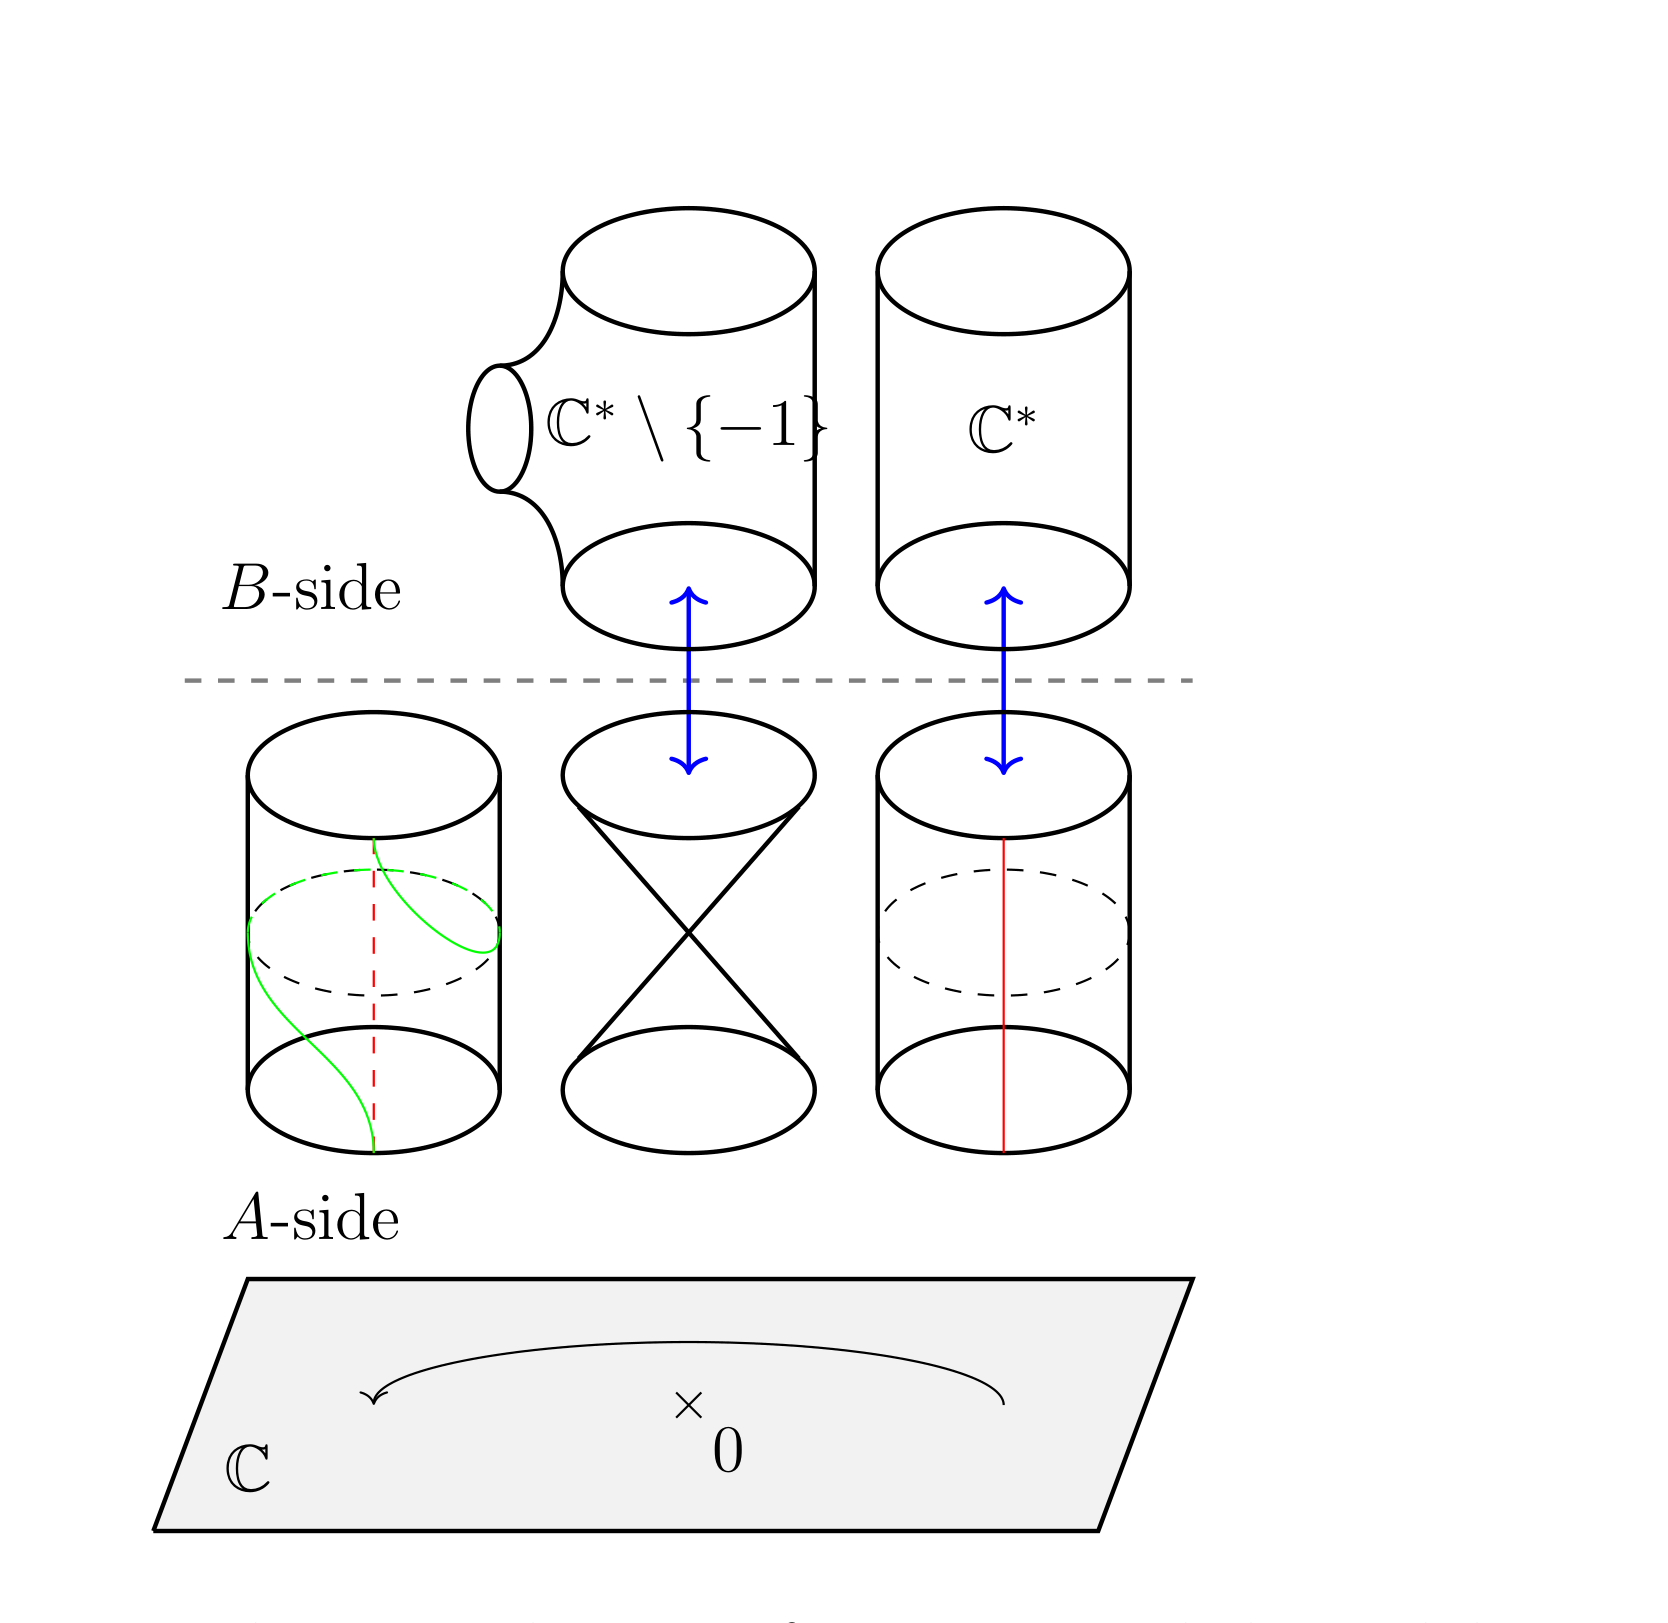
\includegraphics[width=0.60\textwidth]{figures/fig1_1.png}
\caption{裤子 $\Pi_1$ 与结点二次曲线 $\{xy=0\}$ 之间的镜像对称。}
\label{fig:pair-pants}
\end{figure}

最简单的例子是 $\Pi_1$，其镜像是 $\C^2$ 中的结点二次曲线 $\{xy=0\}$。该奇异超曲面的
光滑化是柱面 $\{xy=t\}$，绕 $t=0$ 的单值性由沿结点 vanishing cycle 的 Dehn twist 扭转
给出。HMS 中的一项标准计算给出：柱面的 wrapped Fukaya 范畴由 Laurent 多项式环
$\C[z^{\pm1}]$ 上的有限生成模给出，而 Dehn twist 扭转诱导的自然变换对应乘 $1+z$。

% ===== 原书 p.5 =====
在这条自然变换处作局部化，等于让 $1+z$ 可逆；这确实给出裤子 $\C^*\setminus\{-1\}$ 上的
函数环（见图 \ref{fig:pair-pants}）。

\transnote{背景直觉：柱面 $\{xy=t\}$ 的 wrapped Fukaya 范畴等价于 $\C[z^{\pm1}]$ 上的
有限生成模范畴，生成元 $z$ 对应绕柱面一周的拉格朗日圆圈；乘 $1+z$ 这条自然变换把
$\C[z^{\pm1}]$ 换成 $\C[z^{\pm1},(1+z)^{-1}]$，后者正是 $\C^*\setminus\{-1\}$ 上的函数
环。作者借此把“局部化”落到一个可手算的例子。}

按通常表述，HMS 还有一处问题：它在某种意义上提法不够确定——给定一对范畴之间可能存在许
多等价，其中一些显然涉及作选择。例如，许多 HMS 证明的做法是：在 A 侧与 B 侧各选
一组生成元，再匹配它们的自同态代数。我们如何锁定某一个特定的 HMS 等价？一种回答是：应
当要求 HMS 把 A 侧与 B 侧自然定义的函子相互交织。这类结果此前已见于文献，例如
[HH22; Han19; Nad19b; Can20; HK21]，以及 Cannizzo--Azam--Lee--Liu 的在研工作；此外，
人们早已知道（始于 [PZ98; Fuk02]）阿贝尔簇的镜像对称尊重幺半结构。在本论文第二部分，
我们研究通常镜像对称定理的一种强化：函子性镜像对称试图证明，我们不仅有一个镜像等价，
而且有正确的镜像等价，即它把 A 侧与 B 侧自然定义的函子相互交织。

\transnote{含糊点拨：“正确的镜像等价”不是指唯一性，而是指所取的等价同时与两侧的自然
函子相容；作者把这一要求称为函子性镜像对称，并以“交织”（intertwine）说明函子与等价
之间的交换关系。}

Auroux 在 [Aur18] 中注意到：极仿射超曲面 $H$ 的补集 $(\C^*)^n\setminus H$ 本身是
$(\C^*)^{n+1}$ 中的极仿射超曲面，并且 $H$ 的镜像对称应当与 $(\C^*)^n\setminus H$ 的镜
像对称相关联。在本论文第二部分（与 Benjamin Gammage 的合作工作），我们发现极仿射超曲
面的补集其实有两个自然镜像，其中之一是导出概型。这两个镜像由一个以 Orlov 导出
Kn{\"o}rrer 周期性为中介的非几何等价相联系。

% ===== 原书 p.6 =====
在本论文第二部分，我们随后用这些想法证明 Auroux 的函子性镜像对称猜想：极仿射超曲面及
其补集的同调镜像对称，尊重 A 侧与 B 侧某些自然定义的函子。

\subsection{奇异超曲面}

在本论文第一部分，我们证明：采用 Auroux 的定义，奇异超曲面（在\emph{大复结构极限}处）
的深谷范畴确实满足所预期的同调镜像对称等价。我们还证明 Orlov 的一个猜想：这些奇异超曲
面的深谷范畴满足其\emph{导出} Kn{\"o}rrer 周期性定理的辛类比。这些结果为研究 HMS 开辟
了新途径——使我们能够研究非常一般的一类奇异簇的 A 模型。此外，它还解释了某些簇何以会
有若干个不同维数的镜像。

概括 Auroux 的定义如下。设 $X$ 是 Stein 流形。对只有一个奇异纤维（位于 $0$ 上方）的奇
异辛纤维丛 $f\colon X\to\C$，Seidel [Sei09b; Sei12] 定义了一条自然变换
$s\colon\mu\to\id$，其中 $\mu$ 是作用在一般纤维的 wrapped Fukaya 范畴
$\cW(f^{-1}(t))$ 上的顺时针单值函子（定义见 §2）。Auroux 提出了下述奇异纤维的 wrapped
Fukaya 范畴的定义：

\begin{definition}[Auroux]\label{def:sing-fuk}
设奇异辛纤维丛 $f\colon X\to\C$ 恰有一个奇异纤维，位于 $0$ 上方。则 $f^{-1}(0)$ 的
wrapped Fukaya 范畴定义为：在自然变换 $s\colon\mu\to\id$ 处，对充分小的 $t\neq0$ 取邻
近纤维 $f^{-1}(t)$ 的 wrapped Fukaya 范畴的局部化：
\[
D\cW(f^{-1}(0))=D\cW(f^{-1}(t))[s^{-1}].
\]
\end{definition}

% ===== 原书 p.7 =====
此处是 [LO06] 意义下 $A_\infty$ 范畴的局部化，而 $D$ 表示扭复形的范畴。这一定义也可推
广到单调纤维的情形，或任何 Seidel 自然变换有定义的场合。

\transnote{易错预警：$D$ 是扭复形范畴的记号，与后文的 $D^\pi$（幂等完备的扭复形范畴）
不同；两者在原文中都是数学斜体的 $D$，不要误排成花体 $\cD$（花体 $\cD$ 在本论文中另指
一个满子范畴，见 §1.3.1 末段）。}

在本论文第一部分，我们将证明若干结果，以说明这确实就是奇异超曲面的深谷范畴的正确定义：
Orlov 导出 Kn{\"o}rrer 周期性定理的一个 A 侧类比（定理 \ref{thm:knorrer}），以及若干
大复结构极限处的同调镜像对称等价（定理 \ref{thm:lcsl}）。这些结果将在随后各节详述。

我们将在 §2.3 给出一个启发式说明，解释定义 \ref{def:sing-fuk} 与 Biran--Cornea 拉格朗
日配边群的一个版本之间何以有非常自然的关系。此外还可以构造“邻近圈”函子的一个自然类
比，它把拉格朗日子流形从奇异纤维的去心邻域的 wrapped Fukaya 范畴，限制到奇异纤维自身
的 wrapped Fukaya 范畴（见 §8）。

\subsection{Kn{\"o}rrer 周期性}

关于奇异超曲面深谷范畴的第一个定理，其灵感来自 Orlov 的导出 Kn{\"o}rrer 周期性定理
[Orl06a, Corollary 3.2]。该定理断言：若 $X$ 是光滑拟射影簇，$f\colon X\to\C$ 是正则函
数且 $f^{-1}(0)$ 光滑，则存在范畴等价
\[
\operatorname{Coh}(f^{-1}(0))\to\operatorname{Sing}(X\times\C,zf),
\]
其中 $z$ 是 $\C$ 上的坐标。

% ===== 原书 p.8 =====
[Orl06a] 虽在 $f^{-1}(0)$ 光滑的情形下陈述该定理，但结论对任意超曲面都成立（见 §6.1）：
因此它使我们能用光滑簇 $X\times\C$ 上的 LG 模型来研究这类奇异超曲面。Orlov 在 [Orl06a]
中猜想：同一关系对 A 模型也应成立；与 Orlov 的结果类比，我们或可期望 $f^{-1}(0)$ 的
wrapped Fukaya 范畴，等价于 Landau--Ginzburg 模型 $(X\times\C,zf)$ 的（逐纤维缠绕的）
Fukaya--Seidel 范畴，记作 $\cW(X\times\C,zf)$。这是我们的第一个主要结果。

\transnote{含糊点拨：$\operatorname{Sing}$ 记号的严格含义见 §6.1；在那里作者用矩阵分解
范畴给出它的具体模型。此处只需知道它是 B 侧一个只依赖 LG 模型 $(X\times\C,zf)$ 的范畴，
从而使“奇异纤维的 A 侧”有了“光滑簇上的 LG 模型”这一替身。}

\begin{theorem}[{导出 Kn{\"o}rrer 周期性}]\label{thm:knorrer}
设 $X$ 是光滑仿射簇，带嵌入 $X\to\C^N$，该嵌入在 $X$ 上诱导 Stein 结构；设
$f\colon X\to\C$ 是 $\C^N$ 上多项式函数的限制。若 $f$ 只有一个临界纤维 $f^{-1}(0)$，
则对充分小的 $t\neq0$，存在 $A_\infty$ 范畴的拟等价
\[
D^\pi\cW(f^{-1}(t))[s^{-1}]\to D^\pi\cW(X\times\C,zf).
\]
\end{theorem}

此处 $D^\pi$ 表示扭复形的幂等完备化；我们预期，若不取幂等完备化，该结果不成立。几何假
设几乎肯定可以减弱，但现有的假设已足以用于镜像对称的应用。

% ===== 原书 p.9 =====
注意，对 LG 模型而言，这是与奇点理论中通常考虑的“悬置”或“周期性”不同的一种形式（比
较 [Sei09a]）。

\transnote{含糊点拨：原文强调“不同的一种形式”，指通常的悬置把一个 LG 模型换成另一个、
不改变奇异纤维的等价类；而这里把奇异纤维 $f^{-1}(0)$ 的范畴与高一维的 LG 模型
$(X\times\C,zf)$ 的范畴等同起来，方向相反，故作者特别提醒不要混同。}

上述结果未必局限于奇异超曲面。对奇异完全交，我们可以作如下定义：

\begin{definition}\label{def:sing-ci}
设 $f_1,\dots,f_k\colon X\to\C$ 是 Stein 流形上的全纯函数，且当
$t_1,\dots,t_k\neq0$ 时，交 $f_1^{-1}(t_1)\cap\cdots\cap f_k^{-1}(t_k)$ 光滑。则定义
\[
D\cW(f_1^{-1}(0)\cap\cdots\cap f_k^{-1}(0))
=D\cW(f_1^{-1}(t_1)\cap\cdots\cap f_k^{-1}(t_k))[s_1^{-1},\dots,s_k^{-1}],
\]
其中 $s_i$ 是 $f_i$ 绕 $t_i=0$ 的单值性给出的自然变换，$t_i$ 充分小。
\end{definition}

把我们的证明迭代下去，我们还预期主定理可以简单推广到奇异完全交：

\begin{conjecture}\label{conj:sing-ci}
在关于 $f_1,\dots,f_k$ 的适当假设下，存在 $A_\infty$ 范畴的拟等价
\[
D^\pi\cW(f_1^{-1}(0)\cap\cdots\cap f_k^{-1}(0))
\simeq D^\pi\cW(X\times\C^k,z_1f_1+\cdots+z_kf_k),
\]
其中 $z_1,\dots,z_k$ 是 $\C^k$ 上的坐标。
\end{conjecture}

下文将讨论如何通过推广本论文的结果来证明这一猜想。

\transnote{易错预警：定义 \ref{def:sing-ci} 的显示公式中，左侧各 $f_i$ 取 $0$，右侧各
$f_i$ 取 $t_i$，且局部化要同时在 $k$ 条自然变换处进行，写 $[s_1^{-1},\dots,s_k^{-1}]$；
不要漏掉下标或误写成单个 $s^{-1}$。}

\subsubsection{Kn{\"o}rrer 周期性定理的证明概要}

% ===== 原书 p.10 =====
我们首先在我们的框架下，给出 Abouzaid--Auroux--Katzarkov 一个定理
[AAK16, Corollary 7.8] 的强化形式之证明，该结果或许有独立的价值：

\begin{theorem}[{Abouzaid--Auroux--Katzarkov 等价}]\label{thm:aak-equiv}
设 $X$ 是光滑仿射簇，带嵌入 $X\to\C^N$，该嵌入在 $X$ 上诱导 Stein 结构；设
$f\colon X\to\C$ 是 $\C^N$ 上多项式函数的限制。若 $f$ 只有一个临界纤维 $f^{-1}(0)$，
则对充分小的 $t\neq0$，存在 $A_\infty$ 范畴的拟等价
\[
T\colon\cW(f^{-1}(t))\to\cW(X\times\C,z(f-t)),
\]
它由在奇异轨迹 $f^{-1}(t)$ 中的可容拉格朗日子流形上取顶针给出。
\end{theorem}

\transnote{背景直觉：顶针（thimble）是沿一条路径“扫过”的拉格朗日圆盘，其边界落在
Lefschetz 纤维的消失圈上；作者用“在可容拉格朗日子流形上取顶针”描述这个函子 $T$，直观
上就是把 B 侧的 LG 模型沿临界轨迹切出的拉格朗日球面搬到 A 侧。}

在 [AAK16] 中，人们预期这是一个范畴等价，其前提是 Abouzaid--Ganatra [AG] 的一个生成性
结果，而后者应当由命题 \ref{prop:3-0-5} 推出。类似的结果可参看 [AS15, Lemma A.26]。这
一定理或可视为 LG--CY 对应的开弦类比。

\transnote{含糊点拨：LG--CY 对应把 LG 模型的 B 侧与一个卡拉比–丘流形的 A 侧联系起来；
这里是它的“开弦”版本，即把两侧的范畴（而非仅数值不变量）进行比较。}

还有这一陈述的相对版本，它针对逐纤维带停点的 Fukaya--Seidel 范畴，并镜像 Orlov 的一个
结果：

\begin{theorem}\label{thm:relative}
设 $X$ 是光滑仿射簇，带嵌入 $X\to\C^N$，该嵌入在 $X$ 上诱导 Stein 结构；设
$f,g\colon X\to\C$ 都是 $\C^N$ 上多项式函数的限制。若 $f$ 只有一个临界纤维
$f^{-1}(0)$，则对充分小的 $t\neq0$，存在全忠实函子
\[
\cW(f^{-1}(t),g)\to\cW(X\times\C,z(f-t),g).
\]
\end{theorem}

% ===== 原书 p.11 =====
此处第二个范畴关于 $g$ 逐纤维带停点，详见定义 \ref{def:4-1-1}。

由此还应能推出定理 \ref{thm:knorrer} 的相对版本，进而推出猜想 \ref{conj:sing-ci}：

\begin{conjecture}\label{conj:relative}
设 $f\colon X\to\C$ 是 Stein 流形 $X$ 上的全纯函数，且恰有一个临界纤维 $f^{-1}(0)$；
设 $g\colon X\to\C$ 是另一全纯函数。则对充分小的 $\delta,|t|>0$，存在 $A_\infty$ 范畴
的拟等价
\[
D^\pi\cW(f^{-1}(t),g)[s^{-1}]\to D^\pi\cW(X\times\C,zf+\delta g).
\]
\end{conjecture}

我们随后将在 §3 说明：通过仔细分析一般纤维在 $t$ 变化时的 Liouville 几何，从
$(X\times\C,z(f-t))$ 过渡到 $(X\times\C,zf)$ 可以改述为一次去停点（stop removal）。于是，
由 [GPS19; Syl19a] 的去停点定理，范畴 $\cW(X\times\C,zf)$ 可由范畴
$\cW(X\times\C,z(f-t))$ 对一个由环绕圆盘组成的满子范畴 $\cD$ 取商得到。最后，我们在 §4
证明：在定理 \ref{thm:aak-equiv} 的函子 $T$ 之下，$\cW(f^{-1}(t))$ 上自然变换
$\mu\to\id$ 的各锥的本质像，用 K{\"u}nneth 型论证可分裂生成与 $\cD$ 相同的满子范畴。
于是得到定理 \ref{thm:knorrer}。

\transnote{含糊点拨：停点（stop）是流形上允许拉格朗日对象“终结”的边界区域；把停点去掉
（stop removal）会使范畴变小，在形式上表现为对某个满子范畴取商。作者在此把
$z(f-t)$ 到 $zf$ 的变化解释为停点的移动，正是不变量在此处的几何来源。}


% EN49 c02 | 原书 p.12–21（PDF 23–32） | 第 1 章 §1.4–1.5
% 骨架文件：标题行已设定，正文由译者填写。每页起首用 % ===== 原书 p.N ===== 注释标记。
\subsection{大复结构极限处的镜像对称}

% ===== 原书 p.12 =====
上文给出的奇异超曲面的深谷范畴的定义，显然依赖于磨光（smoothing）的选择。这不仅是合意的，而且对同调镜像对称而言至关重要。经典地，镜像对称是凯勒流形与大复结构极限（large complex structure limit，LCSL）复流形族之间的关系。同调镜像对称被预期为一个对合，因此有必要为该族的奇异纤维的深谷范畴建立一个概念。既然镜像的选择依赖于整个退化，奇异纤维的深谷范畴之定义应当涉及磨光的数据，也就不足为奇了。

\transnote{易错预警：原文说同调镜像对称“被预期为一个对合”（expected to be an involution），意思是镜像对称操作两次应回到原处，而不是说它作为函子是自同构。这一预期正是必须为奇异纤维本身定义深谷范畴的理由：若只在邻近纤维上定义，A 侧就无法与 B 侧对称地取镜像。}

另一方面，孤立超曲面奇点的芽具有光滑且连通的 versal 形变空间 [KM98, p. 144]，故一个简单的同伦论证表明：此时（芽的）深谷范畴与磨光的选择无关。因此它给出孤立超曲面奇点的一个（可能有趣的）辛不变量。一般情形下必须提供额外数据，深谷范畴才能被唯一确定：§5 给出了例子。来自镜像对称的预期表明，这一额外数据应采取 $f^{-1}(0)$ 上对数结构（log structure）的形式，因为在好的情形下它被预期决定 $f^{-1}(0)$ 的一个磨光。利用 Parker 的爆炸流形（exploded manifolds）上全纯曲线理论，或许可以为带对数结构的奇异超曲面内蕴地构造 wrapped Fukaya 范畴（某些对数概型具有爆炸流形的结构 [Par12]）。

\transnote{含糊点拨：对数结构（log structure）在这里只是一个来自镜像对称的\emph{预期}，原文并未给出其定义或构造。它大致上记录边界除子与极点的数据，从而补充“沿哪个方向磨光”的信息；把它当作“把磨光唯一确定下来所需的额外数据”来读即可。}

% ===== 原书 p.13 =====
换个角度，从 LG 模型 $(X\times\C,zf)$ 来看，临界轨迹 $f^{-1}(0)\times\C$ 带有 $(-1)$-平移辛结构（$(-1)$-shifted symplectic structure）：我们猜想这一额外结构也足以确定 wrapped Fukaya 范畴，而后者可以用 Joyce 的 $d$-临界轨迹（$d$-critical loci）理论 [Joy15] 等框架内蕴地构造。

\transnote{易错预警：“$(-1)$-平移辛结构”中的平移量 $(-1)$ 是移位辛几何里的移位次数，与“负一次”或“倒数”无关；不要读成辛形式的次数为 $-1$。$d$-临界轨迹的 $d$ 同样是理论的名字（Joyce 的 $d$-critical loci），不是微分符号。}

当辛侧是形如 $(X\times\C,zf)$ 的 LG 模型时，镜像对称的结论可借定理 \ref{thm:knorrer} 改写成关于奇异簇 $f^{-1}(0)$ 的镜像对称陈述。例如，Nadler 的两篇论文 [Nad19a; Nad17] 研究了 $(\C^{n+1},z_1\cdots z_{n+1})$ 的 A 模型的微局部版本。在此情形下，我们的周期性定理有另一种证明，我们将在 §5.1 中概述；此外还可以用 Abouzaid–Auroux 的工作 [AA21]，以我们的术语给出 Nadler 结果的一个简单证明。我们借用即将问世的 [AA21] 续篇中的想法，说明我们的定义如何使这一点推广到环簇中超曲面的补集的情形。

这是更一般的镜像对称陈述的一个特例，后者可在 Gross–Siebert 纲领的框架下理解（记号见 §5.3）。设 $B$ 是整仿射流形，带有多面体分解 $\cP$ 以及严格凸整分段线性多值函数 $\varphi$ 的选择，并令 $(\check B,\check\cP,\check\varphi)$ 为离散 Legendre 对偶数据。再令 $\cX_\varphi\to D$ 与 $\check\cX_{\check\varphi}\to D$ 分别是 Gross 与 Siebert 构造的 $X(B)=TB/T^{\Z}B$ 与 $X(\check B)=T\check B/T^{\Z}\check B$ 的环簇退化。大体积极限是补集 $X(B)\setminus s^{-1}(0)$，其中 $s$ 是联系于 $\varphi$ 的丰富线丛 $\cL_\varphi$ 的一个截面；而大复结构极限是某个环簇退化的中心纤维 $\cX^0_\varphi$。

\begin{theorem}[{大复结构极限与大体积极限的镜像对称}]\label{thm:lvl-lcsl}
当 $B=M_\R/\Gamma$ 是整仿射环面，带有多面体分解 $\cP$，并取定严格凸分段线性多值函数 $\varphi$（其斜率为整）时，大复结构极限 $\check\cX^0_{\check\varphi}$ 同调镜像于大体积极限 $X(B)\setminus s^{-1}(0)$，即存在范畴的拟等价
\[
\mathrm{D}^\pi\cF(\check\cX^0_{\check\varphi})\simeq\mathrm{D}^b\operatorname{Coh}(X(B)\setminus s^{-1}(0)).
\]
\end{theorem}

\transnote{易错预警：花体 $\cX_\varphi$、$\check\cX_{\check\varphi}$ 记环簇退化的\emph{全族}，罗马体 $X(B)$、$X(\check B)$ 记其一般纤维；中心纤维是 $\cX^0_\varphi$（上标 $0$，花体），不能与 $X(B)$ 混同。定理中的 $D$ 是退化族的底，不是除子。}

% ===== 原书 p.14 =====
该定理的一个推论是：带 $n$ 个结点的椭圆曲线的 Fukaya 范畴，与带 $n$ 个穿孔的椭圆曲线的导出相干层范畴之间，存在一个镜像对称陈述。据我们所知，这些同调镜像对称的实例此前并不为人所知。更一般地，我们有

\begin{theorem}[{大复结构极限处的镜像对称}]\label{thm:lcsl}
给定 $X(B)$ 与 $X(\check B)$ 之间的一个同调镜像对称等价，它把绕 $X(\check B)$ 的大复结构极限的（顺时针）单值函子 $\mu$ 与 $X(B)$ 上线丛 $\cL^{-1}$ 的张量积等同起来，且 $\cL$ 的第一 Chern 类 $c_1(\cL)$ 就是 $X(B)$ 上凯勒形式所在的类；则 $X(\check B)$ 的大复结构极限 $X_0(\check B)$ 同调镜像于 $X(B)$ 的某个大体积极限：
\[
\mathrm{D}^\pi\cF(X_0(\check B))\simeq\mathrm{D}^b\operatorname{Coh}(X(B)\setminus s^{-1}(0)),
\]
其中 $s$ 是 $\cL$ 的截面。
\end{theorem}

\transnote{易错预警：定理 \ref{thm:lcsl} 中的大复结构极限写作 $X_0(\check B)$（罗马体 $X$ 带下标 $0$），与定理 \ref{thm:lvl-lcsl} 的花体 $\check\cX^0_{\check\varphi}$ 指同一类对象，只是记号不同。原文如此，照译，不要自行统一。另：$X(B)$ 与 $X(\check B)$ 是互为镜像的一对环簇，$\check B$ 上的数据才对应 $B$ 侧，方向容易读反。}

应用定理 \ref{thm:lcsl} 所需形式的同调镜像对称等价，被预期可由 Abouzaid 的族 Floer 理论结合 Gross–Siebert 纲领的想法推出（见 [GS16]）。§5.3 给出了进一步解释：这些论证必然带有某种启发性质，忽略了局部系统、brane 结构等要点。

% ===== 原书 p.15 =====
等等。定理 \ref{thm:lcsl} 应被当作一个例证：定义 \ref{def:sing-fuk} 应当给出所预期的那些镜像对称等价。

\begin{remarkx}\label{rem:lvl-direction}
证明同调镜像对称的许多策略，与定理 \ref{thm:lcsl} 的方向相反：先证明大复结构极限（LCSL，在 B 侧）与大体积极限（LVL，在 A 侧）之间的等价，再用形变理论的论证推出邻近纤维的同调镜像对称。虽然理解 LVL 的深谷范畴比理解邻近纤维的更容易，但 LCSL 是奇异簇，其深谷范畴不能按常规方式定义，只能借助邻近纤维来定义。这为两种进路之间的差别提供了一些理由；当然，可以把两种进路结合起来，以获得对模空间上各点处同调镜像对称的理解。
\end{remarkx}

\transnote{背景直觉：注 \ref{rem:lvl-direction} 点出了本论文与既有文献的分工。传统路线是“先在极限处证等价，再形变到一般纤维”；本文的路线是把奇异纤维的深谷范畴本身定义好，从而让“极限处的等价”就是一个关于奇异簇的陈述。两条路线合起来覆盖整个模空间。}

\subsection{环簇的镜像对称}

本论文的许多结果都在环簇 Fano 簇的镜像对称背景下展开，这里先作回顾。设 $H\subseteq(\C^*)^n$ 是光滑代数超曲面（即极仿射超曲面），并取 $n$ 元 Laurent 多项式 $f$，使 $H=f^{-1}(0)$。我们将 $f$ 写成如下形式
\[
f(z)=\sum_{\alpha\in A}c_\alpha T^{\varphi(\alpha)}z^\alpha
\]
其中 $A\subseteq\Z^n$ 是 $f$ 中所有单项式的多重指标之集；$c_\alpha$ 暂时取为任意非零复数；$T$ 是一个小实数；$\varphi$ 是函数 $A\to\R$。设 $P$ 是 $\R^n$ 中由 $A$ 的凸包给出的多面体；于是要求 $\varphi$ 是 $P$ 上某个凸分段线性函数的限制，而后者的线性性极大区域给出 $P$ 的一个多面体分解，其顶点恰为 $A$ 中的点。

\transnote{易错预警：$T^{\varphi(\alpha)}$ 中的 $T$ 是一个小实数，充当退化参数（相当于 SYZ 图景中的尺度）；$\varphi$ 才是分段线性函数，两者不要与温度、周期或平移混淆。取 $T\to0$ 时，各项按 $\varphi(\alpha)$ 的大小分层，这正是热带极限的来源。}

% ===== 原书 p.16 =====
我们将进一步要求 $f$ 满足以下条件：
\begin{enumerate}[label=\arabic*.,leftmargin=2em,itemsep=0.2em]
\item $A$ 的所有非零点都落在 $P$ 的边界上；
\item 由 $\varphi$ 诱导的 $P$ 的多面体分解是极大的（分解的所有胞腔在 $\GL_n(\Z)$ 作用下都与标准单纯形合同）；
\item Laurent 多项式 $f$ 有常数项，即 $0\in A$，且 $0$ 是分解中每个极大胞腔的顶点。
\end{enumerate}

\transnote{含糊点拨：条件 (2) 中的“极大”（maximal）不是“胞腔数目最多”，而是指该多面体分解在加细意义下不能再细分：每个胞腔都是与标准单纯形合同的整多面体。条件 (1) 则把 $f$ 的支撑限制在 $P$ 的边界上，这保证 $H$ 在 $(\C^*)^n$ 中的紧化只沿边界方向退化。}

上文中，多面体 $P$ 的边界带有一个多面体分解；令 $\Sigma_X$ 为由该分解各面所张的锥构成的环簇扇。此扇的射线由 $A\subseteq\Z^n$ 中的向量生成。设 $X$ 是相应的复环簇；令 $i_D\colon D\to X$ 为环簇反典范除子的包含，该除子是反典范丛 $\cK_X^{-1}$ 的一个截面 $s$ 的零点轨迹。我们用 $\cK_X$ 记 $X$ 上作为层的典范丛，并用 $K_X$ 记典范丛的全空间；$K_X$ 也是环簇，其扇 $\tilde\Sigma_X\subseteq\R^{n+1}$ 的射线由 $(1,-\alpha)$（$\alpha\in A$）生成，且 $(1,-\alpha_i)$ 张成一个锥，当且仅当 $\alpha_i$ 张成由 $\varphi$ 诱导的多面体 $P$ 的分解中的一个胞腔。此外，令 $\tilde S$ 记 $X\times\mathbb A^1$ 内的环簇反典范除子，并令 $\hat Z$ 记 $K_X\times\mathbb A^1$ 内的环簇反典范除子（即典范丛的典范丛中的“大反典范除子”）。再令 $X\times\mathbb A^1[-1]$ 记导出概型，其中 $\mathbb A^1[-1]=\operatorname{Spec}\C[t]$，$t$ 的度为 $-1$。我们将用 $\tilde Z$ 记把 $X\times\{0\}$ 沿 $D$ 粘到 $D\times\mathbb A^1[-1]$ 上所得的导出概型。

\transnote{易错预警：$\cK_X$ 与 $K_X$ 只差一个花体，含义却不同——花体记 $X$ 上\emph{作为层}的典范丛，直立体记典范丛的\emph{全空间}（一个环簇）。原文正是用这一对记号区分层与全空间，译文中不可合并。}

\transnote{易错预警：$\hat Z$ 与 $\tilde Z$ 形状相近但不同。$\hat Z$ 是 $K_X\times\mathbb A^1$ 内的环簇反典范除子；$\tilde Z$ 是把 $X\times\{0\}$ 沿 $D$ 粘到 $D\times\mathbb A^1[-1]$ 上得到的导出概型。前者是除子，后者是导出概型，粘合的方向也容易读反。}

% ===== 原书 p.17 =====
在上述条件 (3) 下，$X$ 必是光滑的，因此 $\cK_X^{-1}$ 的所有非零截面都是正则的。

假设 (1) 与 (2) 将保证镜像的环簇 $X$ 是光滑的。此外，热带阿米巴 $\Pi_f\subseteq\R^n$ 的补集将恰有一个紧分支（由条件 (3)），于是 $z_0f+1$ 的镜像可典范地等同于典范丛 $K_X$；并且取 $T$ 充分小，可使 $f$ 的全部临界点（由条件 (2)）落在 $1$ 的任意小邻域上方 [Aur18]。若愿意在 [GS22] 的环簇叠框架下工作，假设 (1) 与 (2) 可以减弱：我们将在下文对此作说明。就下文的目的而言，我们将取 $\varphi$ 为函数 $\varphi(\alpha)=1$（对每个 $\alpha\in A\setminus\{0\}$）的一个一般小扰动。

\begin{remarkx}\label{rem:stacky}
条件 (2) 可以减弱为只要求多面体分解的胞腔是单纯形，而不必具有最小体积。给定扇 $\Sigma_X$ 以及每条射线的生成元 $\alpha$ 的选择，我们可以联系一个环簇（Deligne–Mumford）叠 $X$ [BCS05]。单纯形假设保证该叠 $X$ 是光滑的。[GS22] 的同调镜像对称定理正是在这一条件下陈述的，本论文的全部结果在叠的情形下仍成立。在此较弱的条件下，$X$ 作为 Deligne–Mumford 叠是光滑的 [GS22]。本论文所用的一切代数几何结果，在此情形下应当同样适用。
\end{remarkx}

$H$ 的补集可用两种自然的方式看作 $(\C^*)^{n+1}$ 中的极仿射超曲面。它可以由 Laurent 多项式 $\tilde f_0=f+z_0^{-1}$ 定义，也可以由 $\tilde f_\infty=z_0f+1$ 定义，其中 $z_0\in\C^*$ 是 $(\C^*)^{n+1}$ 的第一个因子。当然，作为代数簇二者是相同的，我们将它们统称为 $(\C^*)^n\setminus H$。

\transnote{含糊点拨：$\tilde f_0$ 与 $\tilde f_\infty$ 是同一个补集在 $(\C^*)^{n+1}$ 中的两种极仿射描述，区别只在新增的 $z_0$ 方向上的行为：前者在 $z_0=0$ 处有极点，后者在 $z_0=\infty$ 处有极点。二者作为代数簇相同，但下面的分次数据不同，这正是 §1.5 后半部分的要点。}

% ===== 原书 p.18 =====
考虑 $\phi\colon(\C^*)^n\to\R$，$\phi(z)=|\operatorname{Log}(z)|^2$，即 $(\C^*)^n$ 上的标准 Stein 函数；通过限制，$H$ 与 $(\C^*)^n\setminus H\subseteq(\C^*)^{n+1}$ 都具有 Stein 流形的结构，从而是 Liouville 流形，这使我们能够谈论它们的 wrapped Fukaya 范畴。注意，把 $\phi$ 限制到 $(\C^*)^n\setminus H$ 所得的 Stein 结构，与 [Jef22, p.13] 中在 Stein 流形里超曲面的补集上构造的 Stein 结构是简单 Liouville 同伦的。

对我们而言，空间 $\{\tilde f_0=0\}$ 与 $\{\tilde f_\infty=0\}$ 之间的差别，将在于我们赋予它们的分次/Maslov 数据不同——即典范线丛的一个平凡化选择，它确定深谷范畴上的一个 $\Z$-分次。给定超曲面 $H\subseteq(\C^*)^n$，满足 $H=\{f=0\}$ 的函数 $f$ 给出 $H$ 的典范丛的一个平凡化 $\eta$：把
\[
\Omega=\frac{\dd z_1}{z_1}\wedge\cdots\wedge\frac{\dd z_n}{z_n}
\]
写作 $H$ 上的标准全纯最高阶形式，我们便可通过条件 $\eta\wedge\dd f=\Omega$ 来定义 $\eta$。类似地，$\dd\tilde f_0$ 与 $\dd\tilde f_\infty$ 给出 $(\C^*)^n\setminus H$ 的典范丛的平凡化 $\eta_0,\eta_\infty$。具体地，$\eta_0$ 由限制 $\Omega|_{(\C^*)^n\setminus H}$ 得到，而 $\eta_\infty$ 将是 $f^{-1}\Omega|_{(\C^*)^n\setminus H}$。注意 $\eta_0$ 因此可以延拓越过被去掉的纤维 $H$，而 $\eta_\infty$ 不能。把分次从 $\eta_0$ 换到 $\eta_\infty$，相当于用 $f$ 去除 $\eta_0$。就上同调而言，这对应于用类 $[\arg(f)]\in H^1((\C^*)^n\setminus H;\Z)$ 来扭平凡化 $\eta_0$。

这两个平凡化定义了两个\emph{不同的} dg 范畴，我们分别记之为 $\cW_0((\C^*)^n\setminus H)$ 与 $\cW_\infty((\C^*)^n\setminus H)$。注意它们有\emph{不同的对象}：$(\C^*)^n\setminus H$ 中并非每个拉格朗日量对两种分次都有分次提升。或者，我们可以考虑一个\emph{分次 $A_\infty$ 范畴} $\cW_{0,\infty}((\C^*)^n\setminus H)$，其对象进一步限制为那些对两种分次都容许分次提升者。

\transnote{背景直觉：$\eta_0$ 与 $\eta_\infty$ 只差乘以 $f$ 的幂，但前者在 $H$ 上无极点、后者有极点，于是“哪些拉格朗日量能带分次提升”就不同。这正是同一个辛流形上出现两个不同 dg 范畴的机制；$[\arg(f)]$ 这个上同调类则度量了两种分次之间的扭结。}

% ===== 原书 p.19 =====
当然，还可以考虑 $(\C^*)^n\setminus H$ 上的其他分次结构，但这些结构从 B 侧的观点看不太自然。

\begin{remarkx}\label{rem:framing}
需要注意的是：选取 Laurent 多项式 $f$，就为 $H$ 提供了 $(\C^*)^n$ 内部的一个标架（framing）。
\end{remarkx}

我们将使用如下术语：Liouville 流形 $X$ 的\emph{扇形分解}（sectorial decomposition）或\emph{扇形粘合}（sectorial gluing），是指 $X$ 中的一个扇形超曲面 $F$，使得 $X$ 是两个 Liouville 扇形 $X_1,X_2\subseteq X$ 的并，且二者沿其边界相交，$\partial X_1=\partial X_2=F$。

下文中，所有 dg/$A_\infty$ 范畴都取为 $\C$-线性的（照常带有其内部/上同调 $\Z$-分次）；所谓\emph{分次 dg 范畴}（或 $A_\infty$ 范畴），指带有\emph{额外} $\Z$-分次的 dg 范畴；换言之，dg 范畴上的一个分次，就是一个 $\operatorname{Coh}(B\mathbb G_m)$-线性结构。dg 范畴上的一个\emph{2-周期性结构}（2-periodicity structure）是 $\C((\beta))$-线性结构的一个选择，其中 $|\beta|=2$；\emph{2-周期 dg 范畴}则指容许 2-周期性结构的 dg 范畴。等价地，把该 $\C((\beta))$-线性 dg 范畴在自然变换 $\beta$ 处局部化，便得到一个微分 $\Z/2$-分次范畴。对 $A_\infty$ 范畴，把同调分次模 $2$ 约化，就得到 $\C((\beta))$-线性的 $A_\infty$ 范畴；我们将用横杠表示同调分次模 $2$ 的约化：例如 $\overline{\cW}_0((\C^*)^n\setminus H)$ 与 $\overline{\operatorname{Coh}}(Z)$。$A_\infty$ 范畴的等价，特别会通过把分次模 $2$ 约化而下降到 $\C((\beta))$-线性 $A_\infty$ 范畴的层面。

\transnote{易错预警：$\overline{\cW}_0$、$\overline{\operatorname{Coh}}(Z)$ 上的横杠表示“同调分次模 $2$ 约化”，不是复共轭，也不是闭包或 Zariski 闭包。约化之后分次只到 $\Z/2$，这些范畴才成为 $\C((\beta))$-线性的。}

下文中，对簇 $X$，$\operatorname{Coh}(X,0)$ 将记零的矩阵分解，即相干层范畴 $\operatorname{Coh}(X)$ 的一个 $\C((\beta))$-线性版本。正如我们将在 §6.1 中解释的，可以把 $\C$-线性 dg 范畴 $\operatorname{Coh}(X)$ 作为分次零矩阵分解的范畴恢复出来；我们将后一范畴记作 $\operatorname{Coh}_{\mathbb G_m}(X,0)$。这个 $\mathbb G_m$ 作用的几何意义将在 §6.1 中解释。

% ===== 原书 p.20 =====
读者可参阅附录 A 中关于概型间态射的记号。此后，除非另有说明，下文所有函子都将是 $\Z$-分次范畴之间的 $\Z$-分次函子（即 dg 范畴之间的 dg 函子）。全文中 $\cW$ 将记 [GPS20a] 意义下（部分）wrapped Fukaya 范畴上扭复形的 $A_\infty$ 范畴；$\operatorname{Coh}$ 将记相干层的 dg 导出范畴。所有函子都取导出函子，所有余极限都应在适当的同伦意义下理解。

\subsubsection{函子式镜像对称}

对我们来说最重要的函子式镜像对称示例，是环簇中反典范除子的镜像对称：据多位作者的工作 [Abo06; Abo09; FLTZ12; Han19; Kuw20; Zho19]，对环簇 $X$（满足 §1.5 上文所列的某些假设），存在一个 Landau–Ginzburg 镜像 $((\C^*)^n,f)$，使得有拟等价
\begin{equation}\label{eq:lvl-hms}
\cW((\C^*)^n,f)\simeq\operatorname{Coh}(X),
\end{equation}
这里 $\cW$ 表示部分缠绕深谷范畴，$f$ 是 Laurent 多项式。此外，[GS22; Zho20] 用微局部层方法证明了：极仿射超曲面 $H=f^{-1}(0)$ 镜像于环簇反典范除子 $i_D\colon D\hookrightarrow X$。结合 [GPS20c] 中微局部层与 Fukaya 范畴的比较定理，这给出等价
\[
\cW(H)\simeq\operatorname{Coh}(D).
\]
此外，有交换图表 [GPS20c, Example 7.25]：
\begin{equation}\label{eq:cup-square}
\begin{tikzcd}
\cW(H) \arrow[r,"\sim"] \arrow[d,"\cup"] & \operatorname{Coh}(D) \arrow[d,"i_{D,*}"] \\
\cW((\C^*)^n,f) \arrow[r,"\sim"] & \operatorname{Coh}(X),
\end{tikzcd}
\end{equation}
其中 $\cup$ 表示 Abouzaid–Ganatra 的 cup 函子 [GPS20c]，底部的等价是来自 [Kuw20, Theorem 1.2] 并结合作者 [GPS20c] 的工作所得的等价 (1.1)。这是我们证明的各定理的原型：我们证明同调镜像对称尊重镜像对称两侧某些自然定义的函子。

\transnote{背景直觉：交换图表 (1.2) 是全文的“原型”。右侧 $i_{D,*}$ 是除子 $D\hookrightarrow X$ 的推前；左侧的 $\cup$ 是它在 A 侧的对应物——把定义在 $H$（$D$ 的镜像）上的对象“延拓”到 $(\C^*)^n\setminus H$ 上。所谓函子式镜像对称，就是断言这类由几何自然给出的函子，在镜像等价下逐一对得上。}

% ===== 原书 p.21 =====
Auroux 在 [Aur18] 中观察到，补集 $(\C^*)^n\setminus H$ 也是一个极仿射超曲面，镜像于典范丛 $K_X$ 内的环簇反典范除子 $Z$。我们证明的函子性结果将表明，[GS22] 的同调镜像对称等价把往来于 $\cW((\C^*)^n\setminus H)$ 的、由辛几何定义的函子，与来自镜像 $Z$ 的代数几何的各种拉回、推前映射编织在一起。我们将非正式地说：当存在形如 (1.2) 的交换图表时（相对于指定的镜像对称等价），这些函子在\emph{镜像对称下相对应}。这些结果的精确陈述在下文 §1.6 中给出。

% EN49 c03 | 原书 原书 p.22–28（PDF 33–39） | 第 1 章 §1.6–1.7
% 骨架文件：标题行已设定，正文由译者填写。每页起首用 % ===== 原书 p.N ===== 注释标记。
\subsection{函子式镜像对称的结果}

% ===== 原书 p.22 =====
我们的第二组结果，讨论镜像对称 A 侧上各自然函子的函子式镜像对称。这些函子由 Auroux 在 [Aur18] 中草图性地提出，把 $\cW((\C^*)^n\setminus H)$ 与 $\cW(H)$、$\cW((\C^*)^n,f)$ 联系起来：
\begin{itemize}
\item （$\Z/2$-分次）\emph{限制函子} $\rho\colon\cW((\C^*)^n\setminus H)\to\cW(H)$，它把 $(\C^*)^n\setminus H$ 中的拉格朗日量送到该拉格朗日量沿被去掉的纤维 $H$ 的“端”（\ref{def:8-2-3}）；
\item \emph{提升函子} $j\colon\cW(H)\to\cW((\C^*)^n\setminus H)$：沿一条从 $0$ 到 $\infty$、避开 $f$ 全部临界值的射线，把 $H$ 中的拉格朗日量平行移动（\ref{def:9-0-1}）；
\item \emph{无穷远处缠绕函子} $\alpha_\infty\colon\cW((\C^*)^n,f)\to\cW((\C^*)^n\setminus H)$，它开启绕无穷远的缠绕（\ref{def:7-1-3}, (1)）；
\item \emph{绕 $H$ 的缠绕函子} $\alpha_0\colon\cW((\C^*)^n,f)\to\cW((\C^*)^n\setminus H)$，它开启绕被去掉的纤维 $H$ 的缠绕（\ref{def:7-1-3}, (2)）。
\end{itemize}
下文各节将详细构造这些函子的各个版本。Auroux 猜想这些函子应满足关系
\begin{enumerate}
\item $\rho\circ\alpha_0\simeq\cap$；
\item $\rho\circ\alpha_\infty\simeq 0$；
\item $\rho\circ j\simeq\id$；
\end{enumerate}
以及正合三角形

\transnote{背景直觉：四个函子里，$\rho$ 与 $j$ 是“看端”与“平行移动”这类直观操作；$\alpha_0$ 与 $\alpha_\infty$ 则是把 $\cW((\C^*)^n,f)$ 中已有的两类缠绕“打开”的函子。三条关系式的含义是：先开启缠绕再看端，等于 $\cap$、等于零、或等于恒等。}

\transnote{易错预警：$j\cap$ 是函子 $j$ 与 cap 函子 $\cap$ 的复合，不是集合的交。$\cap$ 是 Abouzaid–Ganatra 的 cap 函子，与 §1.5.1 中交换图表 (1.2) 里的 $\cup$ 相对；两者分别对应几何中的 cap 与 cup。}

% ===== 原书 p.23 =====
\[
\begin{tikzcd}[row sep=1.0em, column sep=3.6em]
{j\cap} \arrow[rr,"+1"] & & \alpha_\infty \arrow[dl] \\
& \alpha_0 \arrow[ul] &
\end{tikzcd}
\]

\transnote{含糊点拨：原文只把三角形画出来、未写循环方向。按箭头读，它是 $\alpha_0\to j\cap\xrightarrow{+1}\alpha_\infty\to\alpha_0$：$+1$ 标在从 $j\cap$ 出发的那条箭头上，表示三角的第三个映射带分次移位 $1$。}

Auroux 随后就上述函子及其在代数几何中的镜像提出四条猜想。我们在此复述，并指出本论文讨论各条猜想的章节。

\begin{conjecture}[{[Aur18]}]\label{conj:aur-funct}
以下函子在镜像对称下相对应：
\begin{enumerate}
\item （Conjecture 1.2）函子 $\rho$ 镜像于商函子 $q\colon\operatorname{Coh}(Z)\to\operatorname{Sing}(Z)$ 与 Kn{\"o}rrer 周期性等价 $\operatorname{Sing}(Z)\to\operatorname{Coh}(D)$ 的复合（§8）；
\item （Conjecture 1.3 (1)）函子 $\alpha_0$ 镜像于 $i_{X*}$，其中 $i_X\colon X\to Z$ 是包含（§7）；
\item （Conjecture 1.3 (2)）函子 $\alpha_\infty$ 镜像于 $\pi_X^*$，其中 $\pi_X\colon Z\to X$ 是投影（§8）；
\item （Conjecture, §6.2）函子 $j$ 镜像于 $j_{D*}p_D^*(K_X^{-1}|_D\otimes\cdot\,)$，其中 $j_D\colon K_X|_D\to Z$、$p_D\colon K_X|_D\to D$ 分别是包含与投影（§9）。
\end{enumerate}
\end{conjecture}

\transnote{易错预警：条目开头的“（Conjecture 1.2）”“（Conjecture 1.3 (1)）”是 Auroux 论文 [Aur18] 内部的猜想编号，不是本书编号。译文照字面保留，不要误加 \texttt{\textbackslash ref}。}

本论文在按分次数据作适当修改之后证明这些猜想。本论文第二部分的主要结果可概括如下：

\begin{thmstar}
在 \ref{thm:7-2-4} 所述 [Kuw20] 与 [GS22] 的镜像对称等价，与 \ref{thm:6-1-16} 及 \ref{lem:6-1-7} 的 Kn{\"o}rrer 周期性等价复合之后：
\begin{enumerate}
\item （\ref{thm:7-2-4}, (2)）函子 $\alpha_0\colon\cW((\C^*)^n,f)\to\cW_\infty((\C^*)^n\setminus H)$ 镜像于 $i_{X*}$，其中 $i_X\colon X\to Z$ 是包含；
\item （\ref{thm:8-2-1}）函子 $\alpha_\infty\colon\cW((\C^*)^n,f)\to\cW_0((\C^*)^n\setminus H)$ 镜像于 $\pi_X^*[1]$，其中 $\pi_X\colon Z\to X$ 是投影；
\item （\ref{thm:8-2-5}）函子 $\rho\colon\overline{\cW}_0((\C^*)^n\setminus H)\to\overline{\cW}(H)$ 镜像于商函子 $q\colon\overline{\operatorname{Coh}}(Z)\to\overline{\operatorname{Sing}}(Z)$；
\item （\ref{thm:8-3-6}）$\rho$ 的分次提升 $\cW_{0,\infty}((\C^*)^n\setminus H)\to\overline{\cW}(H)$，是 $q\colon\overline{\operatorname{Coh}}_{\mathbb G_m}(Z)\to\overline{\operatorname{Sing}}_{\mathbb G_m}(Z)$ 的分次提升的（分次）镜像；
\item （\ref{thm:9-0-2}）函子 $j$ 镜像于 $j_{D*}p_D^*$，其中 $j_D\colon K_X|_D\to Z$、$p_D\colon K_X|_D\to D$ 分别是包含与投影。
\end{enumerate}
此外还有正合三角形（\ref{cor:9-0-4}）：

% ===== 原书 p.24 =====
\[
\begin{tikzcd}[row sep=1.0em, column sep=3.6em]
{j\cap} \arrow[rr,"+1"] & & \alpha_0 \arrow[dl] \\
& \alpha_\infty \arrow[ul] &
\end{tikzcd}
\]
\end{thmstar}

\transnote{易错预警：定理中 $\cW_\infty$ 与 $\cW_0$ 的下标，对应 §1.5 定义的两个分次 $\eta_\infty$ 与 $\eta_0$；它们与函子名 $\alpha_\infty$、$\alpha_0$ 的下标一致，但两者是不同层面的对象，不可混同。}

\transnote{含糊点拨：$\overline{\cW}$、$\overline{\operatorname{Coh}}$ 上的横杠，是 §1.5 中由 $A_\infty$ 分次模 $2$ 约化得到的记号，表示微分 $\Z/2$-分次范畴，并非拓扑闭包。}

\begin{remarkx}\label{rem:aur-monodromy}
我们的函子与 Auroux 在 [Aur18] 中所定义的函子，相差一次单值变换的作用：Auroux 定义 $\alpha_0,\alpha_\infty$ 时，要求拉格朗日量都先在底空间沿负实无穷方向作平行移动；我们改以扇形包含来定义 $\alpha_0,\alpha_\infty$，于是拉格朗日量分别直接走向负实无穷与正实无穷（参 [Aur18, Fig. 4]）。这意味着我们的结果有时与 [Aur18] 中的猜想相差一次单值变换的作用（参 \ref{thm:9-0-2}）与一次分次平移。
\end{remarkx}

\subsubsection{函子式镜像对称的证明技巧}

% ===== 原书 p.25 =====
本节稍作启发式地综述本论文第二部分用到的一些主要技巧。第一个技巧是 [GPS19, Theorem 1.28] 中 wrapped Fukaya 范畴的同伦推出（homotopy pushout）定理，以及 [GR17, Proposition 4.7.2.2] 中相干层范畴的真下降（proper descent）定理。

$(\C^*)^n\setminus H$ 有两种表示：$\tilde f_0=0$ 或 $\tilde f_\infty=0$。二者自然给出 $\C$ 上两个（奇异）辛纤维丛，分别由 $f$ 与 $1/f$ 给出；同时也给出 $(\C^*)^n\setminus H$ 作为 Liouville 扇形粘合的两个表示。这两个表示又分别对应两个镜像空间 $\tilde Z$ 与 $Z$ 分解为不可约分支。然而，这种辛粘合难以实现。

\transnote{背景直觉：同伦推出定理在 A 侧负责“拼接”，真下降定理在 B 侧负责“拼接”；两侧的拼法在镜像对称下互相对应，这正是本节全部技巧的骨架。}

\transnote{易错预警：这里的“两个（奇异）辛纤维丛”不是同一个纤维化的两种写法，而是 $f$ 与 $1/f$ 两个不同的纤维化；它们的奇异纤维位置互为颠倒，这正是下文“交换零与无穷”的来源。}

给定仿射簇 $X$ 上的多项式函数 $W\colon X\to\C$ 与 Stein 函数 $\phi\colon X\to\R$，实超曲面 $F=\{\operatorname{Re}(W)=C\}$ 应当是扇形超曲面的原型例子：它把 $X$ 表示成两个扇形 $\{\operatorname{Re}(W)\le C\}$ 与 $\{\operatorname{Re}(W)\ge C\}$ 沿 $F$ 的扇形粘合。借助函数 $I=\operatorname{Im}(W)$，$F$ 满足 [GPS20a, Definition 1.2] 的第二个条件；但该定义隐含要求 $F$ 在无穷远处切于 $X$ 的 Liouville 向量场。这一条件一般无法保证，即便把 $X$ 上的 Liouville 结构作形变也未必可行。存在这种简单 Liouville 形变的判据，将出现在第二作者及合作者的未来工作中。这里我们描述另一种构造，它给出相同的结果（§7）。

\transnote{含糊点拨：“$F$ 满足定义的第二个条件”并不等于“$F$ 是扇形超曲面”：缺的是切于 Liouville 向量场这一条。原文用 while 转折，意在强调这个隐含条件才是障碍。}

接下来，我们不必沿整个超曲面 $F$ 修正 Liouville 结构，而可以应用 Sylvan 的一个结果 [Syl19b, Prop 2.6]，在无穷远处某条纤维的邻域内给出标准 Liouville 形式。

% ===== 原书 p.26 =====
令 $H=W^{-1}(R_1)\cap\{\phi\le R_2-\eps\}$，则该命题给出：对某个 $\rho>0$（且 $R_1,R_2$ 充分大），$H$ 有一个标准 Liouville 邻域
\[
U=\left(\hat H\times\{z\in\C:\operatorname{Re}(z)>-\rho\},\ \lambda_X|_H+\lambda_\C^{\operatorname{std}}\right),
\]
它在完备化 $\hat X$ 中真嵌入（见\ref{fig:7-1}）。须提醒读者：投影 $z\colon U\to\C$ 未必与原映射 $W\colon X\to\C$ 相容，尽管 $z$ 的纤维将与 $W$ 的纤维同痕。

\transnote{易错预警：$H=W^{-1}(R_1)\cap\{\phi\le R_2-\eps\}$ 里的 $R_1$ 与 $R_2$ 是两个不同的大参数，分别控制纤维与截断，不能混同；$\rho$ 也与限制函子 $\rho$ 同名，但此处是正实数。}

\transnote{背景直觉：Sylvan 的命题只保证“无穷远处某条纤维附近”有标准 Liouville 形式，所以 $z$ 只能与原 $W$ 的纤维同痕、而不与之相等。这正是这种构造的代价，也是它的用处。}

于是我们得到 $X$ 内真嵌入的扇形超曲面 $\{\operatorname{Re}(z)=0\}\subseteq U$。在我们的情形中取 $W=f$，这就把 $(\C^*)^n$ 表示成 $((\C^*)^n,f)$ 与 $(H\times\C,z)$ 的平凡粘合。若改在邻域 $U$ 内去掉超曲面 $H$，则 $(\C^*)^n\setminus H$ 可表示成 $((\C^*)^n,f)$ 与 $(H\times\C^*,z)$ 的扇形粘合（\ref{prop:7-1-1}）。

同一论证对函数 $1/W\colon X\to\C$ 不成立，因为 $1/W$ 在 $X$ 上并非处处有定义，也不再是多项式。我们可以换一种做法：在 $W$ 诱导的 $X$ 的扇形分解中“交换零与无穷”，由此构造 $1/W$ 诱导的 $X$ 的扇形分解。更确切地说，这意味着从先前的构造出发，施加由 $f$ 的整体单值性给出的纤维 $H$ 的同痕。应用 [GPS20a] 的唯一性结果可知，总能找到一族“跟随”该同痕的扇形超曲面。所得的扇形分解，把 $(\C^*)^n\setminus H$ 表示成 $((\C^*)^n,f)$ 与 $\C^*$ 上一个 $H$-丛的扇形粘合，该丛由 $f$ 的整体单值性扭成（见\ref{fig:7-6}、\ref{prop:7-1-2}）。

\transnote{易错预警：$1/W$ 的问题不在“值太大”，而在于它在 $X$ 上并非处处有定义、且不再是多项式，故同伦推出定理的前提失效，只能改用单值性扭成的粘合。}

本论文用到的第二个主要技巧，是带规范群的 LG 模型的导出 Kn{\"o}rrer 周期性（参 [Hir17]）。由 $1/f$ 诱导的 $(\C^*)^n\setminus H$ 的扇形粘合，在镜像对称下对应 $Z$ 由其不可约分支的 B 侧粘合（\ref{thm:7-2-4}）；另一方面，非常规的分次 $\eta_0$ 意味着：由 $f$ 诱导的 $(\C^*)^n\setminus H$ 的扇形分解，给出带分次 $\eta_0$ 的 $(\C^*)^n\setminus H$ wrapped Fukaya 范畴与导出概型 $\tilde Z$ 上相干层之间的一个等价。

% ===== 原书 p.27 =====
为把这一结果拉回到 [Aur18] 关于 $Z$ 的原始镜像对称猜想，我们需要 $\operatorname{Coh}(Z)$ 与 $\operatorname{Coh}(\tilde Z)$ 之间的等价。这两个概型由 Koszul 对偶与导出 Kn{\"o}rrer 周期性的组合联系起来：二者有公共的 Kn{\"o}rrer 稳定化，稳定到 $K_X\times\mathbb A^1$ 上 $syz$ 的（分次）矩阵分解范畴，其中 $y,z$ 分别记 $K_X$ 与 $\mathbb A^1$ 的纤维上的坐标（\ref{thm:6-1-16}）。

\transnote{含糊点拨：$\operatorname{Coh}(Z)$ 与 $\operatorname{Coh}(\tilde Z)$ 之间的等价并非恒等，而是经“公共 Kn{\"o}rrer 稳定化”过渡得到的；原文用 stabilization 一词，指两个概型各自再添一对互为对偶的坐标后同构。}

$\operatorname{Coh}(Z)$ 与 $\operatorname{Coh}(\tilde Z)$ 之间的这个等价具有出人意料的性质，使它成为把 $f$ 换成 $1/f$ 的代数类比。该等价把函子 $i_{\tilde X*}$ 送到 $\pi_X^*[1]$（\ref{lem:8-1-2}），反之亦然；因此 A 侧诱导的等价交换函子 $\alpha_0$ 与 $\alpha_\infty$（\ref{thm:8-2-1}），在某种意义上“交换零与无穷”。这类耐人寻味的非几何等价的一般意义，将留待未来工作讨论。

\transnote{背景直觉：“把 $f$ 换成 $1/f$”是 A 侧的整体单值性操作，其在 B 侧的代数类比就是 $\operatorname{Coh}(Z)\leftrightarrow\operatorname{Coh}(\tilde Z)$。会“交换零与无穷”，指两个缠绕函子 $\alpha_0,\alpha_\infty$ 在该等价下互换。}

\subsection{与已发表工作的关系}

本论文的结果取自两篇文章 [Jef22] 与 [GJ22]，后者是与 Benjamin Gammage 的合作工作。下面列出本论文各节的来源：
\begin{itemize}
\item §1 综合了 [Jef22] §1 与 [GJ22] §1 的内容（含与 Benjamin Gammage 的合作工作）；
\item §2 综合了 [Jef22] §2 与 [GJ22] §3.1 的内容（含与 Benjamin Gammage 的合作工作）；
\item §3 对应 [Jef22] 的 §3；
% ===== 原书 p.28 =====
\item §4 对应 [Jef22] 的 §4；
\item §5 对应 [Jef22] 的 §5；
\item §6 对应 [GJ22] 的 §2（与 Benjamin Gammage 的合作工作）；
\item §7 对应 [GJ22] 的 §3（与 Benjamin Gammage 的合作工作）；
\item §8 对应 [GJ22] 的 §4（与 Benjamin Gammage 的合作工作）；
\item §9 对应 [GJ22] 的 §5（与 Benjamin Gammage 的合作工作）；
\item 附录 A 对应 [GJ22] 的附录 A（与 Benjamin Gammage 的合作工作）。
\end{itemize}

\transnote{易错预警：本节两套“§N”不可互换——左边的“§1”指本论文的节，括号前的“§1 of [Jef22]”指 [Jef22] 的节。译文一律照字面保留，读者须按出处区分。}

\clearpage
% EN49 c04 | 原书 原书 p.29–47（PDF 40–58） | 第 2 章 §2.1–2.3
% 骨架文件：标题行已设定，正文由译者填写。每页起首用 % ===== 原书 p.N ===== 注释标记。
\section{定义与约定}

\subsection{正合 Landau--Ginzburg 模型}

% ===== 原书 p.29 =====
首先说明如何把一个正合 Landau--Ginzburg 模型 $(X,W)$ 变成一个 Liouville 扇形，以便讨论它的 Fukaya--Seidel 范畴。

\begin{definition}\label{def:exact-lg}\label{def:2-1-1}
\textbf{正合 Landau--Ginzburg 模型}（exact Landau--Ginzburg model）$(X,W)$ 由以下数据构成：$X$ 是光滑仿射簇，带嵌入 $i\colon X\to\C^N$，该嵌入使 $X$ 成为 Stein 流形，其 Stein 函数 $\phi\colon X\to\R$ 取 $\phi(z)=|z|^2$ 在 $X$ 上的限制；此外还带全纯函数 $W\colon X\to\C$，它是 $\C^N$ 上某个多项式在 $X$ 上的限制。
\end{definition}

\transnote{易错预警：Stein 函数 $\phi$ 由标准欧氏范数 $|z|^2$ 限制得到，与 $W$ 无关；$|W|^2$ 只是实多项式，并不给出 Stein 结构。}

函数 $|W|^2$ 在 $\R^{2N}$ 上定义一个实多项式，而 $X\subseteq\R^{2N}$ 是实仿射代数簇。回忆：$|W|^2$ 在 $p\in\R$ 处的（实）Malgrange 条件，是指存在
% ===== 原书 p.30 =====
$R,\eps,\eta>0$，使得当 $|z|>R$ 且 $\bigl||W|^2(z)-p\bigr|\le\eps$ 时，有
\[
|z|\,\bigl|\nabla_X|W|^2\bigr|>\eta.
\]

\transnote{含糊点拨：Malgrange 条件是「在无穷远处 $\nabla_X|W|^2$ 不退化」的量化形式；三个常数 $R,\eps,\eta$ 彼此关联，不能独立选取。}

\begin{definition}\label{def:non-malgrange}\label{def:2-1-2}
若 $|W|^2$ 在 $p$ 处的 Malgrange 条件不成立，则称点 $p\in\R$ 为 $|W|^2\colon X\to\R$ 的\textbf{非 Malgrange 点}（non-Malgrange point）。类似地，若 $W$ 在 $p$ 处的（复）Malgrange 条件不成立，则称点 $p\in\C$ 为 $W\colon X\to\C$ 的非 Malgrange 点。
\end{definition}

实代数几何中有一个经典结论：使 $|W|^2\colon X\to\R$ 的 Malgrange 条件不成立的 $\R$ 中点只有有限多个（例如见 [Spo02, Remark 3]，再与代数簇 $X$ 取交）。类似地，$W$ 在 $\C$ 中的复非 Malgrange 点都是孤立的。

于是取 $R>0$ 充分大，使 $W$ 的全部临界点与非 Malgrange 点都落在 $|W|^2<R$ 之内。再把 $X$ 上的 Stein 结构 $\phi$ 形变为
\[
\psi_t(z)=\phi(z)+D\left(\frac{t+\phi(z)|W|^{2m}}{1+t\phi(z)|W|^{2m}}\right),
\]
其中 $t\in[0,1]$，$D>0$ 是正常数，$m$ 是正整数。则

\begin{lemma}\label{lem:psi-outward}\label{lem:2-1-3}
当 $R,D,m>0$ 充分大时，$\psi=\psi_0$ 的 Liouville 向量场沿 $|W|^2=R$ 指向外侧。
\end{lemma}

\begin{proof}
需要验证内积
\[
\langle\nabla_X|W|^2,\nabla_X\psi\rangle
=(1+D|W|^{2m})\langle\nabla_X|W|^2,\nabla_X\phi\rangle
+mD|W|^{2m-2}\phi\bigl|\nabla_X|W|^2\bigr|^2
\]
在 $|W|^2=R$ 上处处严格为正。
% ===== 原书 p.31 =====
由 Cauchy--Schwarz 不等式，
\[
(1+D|W|^{2m})\bigl|\langle\nabla_X|W|^2,\nabla_X\phi\rangle\bigr|
\le 2(1+D|W|^{2m})\bigl|\nabla_X|W|^2\bigr||\phi|^{1/2},
\]
因此只要
\[
2(1+D|W|^{2m})<mD|W|^{2m-2}|\phi|^{1/2}\bigl|\nabla_X|W|^2\bigr|
\]
就有 $\langle\nabla_X|W|^2,\nabla_X\psi\rangle>0$。利用
\[
|\nabla_X\phi|\le\bigl|\nabla|z|^2\bigr|=2|z|
\]
可把该不等式改写为
\begin{equation}\label{eq:2-1}
2\left(\frac{1}{D|W|^{2m-2}}+|W|^2\right)
<m|\phi|^{1/2}\bigl|\nabla_X|W|^2\bigr|.
\end{equation}

\transnote{易错预警：由 $|\nabla_X\phi|\le 2|z|$ 推出 (2.1)，这一步只用 $\C^N$ 的标准度量；换用别的 Kähler 度量，其中的常数要跟着变。}
当 Malgrange 条件在 $R$ 处成立时，存在常数 $\eta>0$，使 $|z|\bigl|\nabla_X|W|^2\bigr|>\eta$ 在 $|W|^2=R$ 上成立；若 $R$ 充分大，使 $W$ 在 $|W|^2=R$ 上没有临界点，则该处 $\bigl|\nabla_X|W|^2\bigr|>0$，于是存在常数 $C>0$（依赖于 $R$），使
\[
|W|^2<C|z|\bigl|\nabla_X|W|^2\bigr|.
\]
% ===== 原书 p.32 =====
因此当 $D,m>0$ 充分大时，不等式 \eqref{eq:2-1} 成立。
\end{proof}

类似地，我们还需要知道 $W$ 的平行移动在某个圆盘之外有定义：

\begin{lemma}\label{lem:parallel-transport}\label{lem:2-1-4}
对某个充分大的 $R>0$，辛平行移动在 $|W|^2=R$ 上方的 $W$ 的光滑纤维之间给出正合辛同胚。
\end{lemma}

\begin{proof}
我们沿用 [FSS08, §2] 的论证。由简单计算（参看 [Sei08b, p.213]）可知，只要辛平行移动有定义，它给出的就是正合辛同胚。平行移动向量场总是
\[
\frac{\nabla_X\operatorname{Re}(W)}{\bigl|\nabla_X\operatorname{Re}(W)\bigr|^2}
\]
的单位复数倍，因为 $\nabla_X\operatorname{Im}(W)=J\nabla_X\operatorname{Re}(W)$。由于 $\phi\colon X\to\R$ 是逆紧（proper）的穷竭函数，只需证明平行移动向量场的流线 $\gamma(t)$ 在 $\phi$ 下的像不会在有限时间内逃向无穷。于是考虑导数
\[
\left|\frac{\nabla_X\operatorname{Re}(W)}{\bigl|\nabla_X\operatorname{Re}(W)\bigr|^2}\phi\right|
=\frac{\bigl|\langle\nabla_X\operatorname{Re}(W),\nabla_X\phi\rangle\bigr|}
{\bigl|\nabla_X\operatorname{Re}(W)\bigr|^2}
\le\frac{|\nabla_X\phi|}{\bigl|\nabla_X\operatorname{Re}(W)\bigr|}.
\]
复多项式 $W\colon X\to\C$ 的 Malgrange 条件在 $\C$ 中只有有限多个点处不成立，故存在常数 $C>0$ 与 $R>0$，使
\[
|W|<C|\phi|^{1/2}|\de_XW|
\]
% ===== 原书 p.33 =====
对 $|W|=R$ 成立，其中 $|\de_XW|=\bigl|\nabla_X\operatorname{Re}(W)\bigr|$。另注意在 $\C^N$ 上有
\[
|\nabla\phi|=\bigl|\nabla|z|^2\bigr|=2|\phi|^{1/2},
\]
从而 $|\nabla_X\phi|\le2|\phi|^{1/2}$。因此在 $|W|=R$ 上，对某个常数 $C$ 有
\[
\phi'(t)\le C\frac{\phi(t)}{|W(t)|},
\]
其中 $\phi(t)=\phi(\gamma(t))$。若 $\gamma(t)$ 避开 $W$ 的零纤维，则存在常数 $\beta>0$，使 $1/|W(t)|<\beta$。于是由 Gr{\"o}nwall 不等式，
\[
\phi(t)\le\phi(0)e^{C\beta t},
\]
证毕。
\end{proof}

\transnote{背景直觉：Grönwall 不等式把 $\phi$ 沿流线的增长压到指数级；指数增长在有限时间内有界，因此流线逃不到无穷远。}

我们常常希望换用另一个 Stein 函数来计算深谷范畴。下面记录一条此后反复使用的标准引理；它在文献中只以隐含的形式出现。

\begin{definition}\label{def:simple-liouville}\label{def:2-1-5}
设 $X$ 是带 Liouville 形式 $\lambda$ 的 Liouville 流形。若 Liouville 形式的光滑族 $\lambda_t$（$t\in[0,1]$）满足 $\lambda_0=\lambda$，且各 Liouville 结构 $\lambda_t$ 的骨架之并始终含于某个紧集之内，则称该族为\textbf{简单 Liouville 同伦}（simple Liouville homotopy）。
\end{definition}

\transnote{含糊点拨：条件只要求「骨架之并」落在某个紧集之内，并不要求骨架本身逐点不动，所以允许骨架随 $t$ 移动。}

% ===== 原书 p.34 =====
例如，临界点始终留在紧集之内的一族 Weinstein 函数就满足这一条件。

\begin{lemma}\label{lem:simple-homotopy}\label{lem:2-1-6}
给定 Liouville 流形 $X$ 与简单 Liouville 同伦 $\lambda_t$，所有 Liouville 流形 $(X,\lambda_t)$ 彼此正合辛同胚，且 wrapped Fukaya 范畴 $\cW(X,\lambda_t)$ 彼此拟等价。
\end{lemma}

\begin{proof}
由 [CE12, Proposition 11.8]，对每个简单 Liouville 同伦，存在一族正合辛同胚 $\phi_t\colon X\to X$，满足 $\phi_t^*\lambda_t=\lambda-\de f$（$f$ 紧支），且 $\phi_0$ 为恒同。这给出 Liouville 扇形的一个平凡包含；故由 [GPS19, Lemma 2.6]，该形变给出 $\cW(X,\lambda_0)$ 与 $\cW(X,\lambda_1)$ 之间的拟等价。
\end{proof}

因此，只要只在拟等价意义下考虑深谷范畴（依据 [Sei08b, Corollary 1.14]），我们在证明中就可以自由使用形变后的 Liouville 结构。带停点的情形也有引理 \ref{lem:simple-homotopy} 的类似版本。这一自由度有一个特别好用的应用：

\begin{proposition}\label{prop:convex-boundary}\label{prop:2-1-7}
存在从 Stein 流形 $(X,\phi)$ 到 Stein 流形 $(X,\psi)$ 的简单 Liouville 形变，使得当 $R_1,R_2>0$ 充分大时，子集 $\{|W|^2\le R_1\}\cap\{\psi\le R_2\}$ 的边界为凸。此外，所有纤维 $W^{-1}(z)\cap\{\psi\le R_2\}$ 都经由沿 $|W|^2(z)=R_1$ 的辛平行移动而彼此正合辛同胚；把角磨圆、得到 Liouville 域
% ===== 原书 p.35 =====
$X_0$ 之后，它们仍彼此正合辛同胚。
\end{proposition}

把磨圆参数取得充分小，则 Liouville 域 $X_0$ 的接触边界包含 Liouville 超曲面 $F=W^{-1}(R_1)\cap\{\psi\le R_2-\eps\}$，且 $F$ 的边界为凸；还可取 $\eps>0$ 充分小，使 $F$ 的完备化与 $W^{-1}(R_1)$ 正合辛同胚。数对 $(X_0,F)$ 给出一个缝合 Liouville 域（sutured Liouville domain），它与充分大的 $R_1,R_2$ 无关。由 [GPS20a, Lemma 2.32]，缝合 Liouville 域对应一个（同伦意义下）唯一的 Liouville 扇形；我们把它记作 $(X,W)$。

\begin{definition}\label{def:liouville-sector}\label{def:2-1-8}
Landau--Ginzburg 模型 $(X,W)$ 所对应的 Liouville 扇形 $(X,W)$，是指（磨圆后的）缝合 Liouville 域
\[
\bigl(\{|W|^2\le R_1\}\cap\{\psi\le R_2\},\ W^{-1}(R_1)\cap\{\psi\le R_2-\eps\}\bigr)
\]
在 $R_1,R_2>0$ 充分大、$\eps>0$ 充分小时所对应的 Liouville 扇形的（等价类）。
\end{definition}

\begin{definition}\label{def:fs-category}\label{def:2-1-9}
$(X,W)$ 的\textbf{Fukaya--Seidel 范畴}，记作 $\cW(X,W)$，是指上述 Liouville 扇形 $(X,W)$ 依 [GPS20a] 意义的部分缠绕深谷范畴。
\end{definition}

这里要说明：把缝合 Liouville 域变成 Liouville 扇形有两种构造。其一是 [GPS20a, Definition 2.14] 所述的“完备化”。另一种是对 $F=W^{-1}(R_1)\cap\{\psi\le R_2-\eps\}$ 应用 [Syl19b, Prop 2.6]；在可能增大 $R_1,R_2$ 之后，由此得到 $F$ 的一个标准 Liouville 邻域 $U$，其形如
\[
\bigl(\hat F\times\{z\in\C:\operatorname{Re}(z)>-\rho\},\ \lambda_X|_F+\lambda_{\C}^{\mathrm{std}}\bigr),
\]
并真嵌入于完备化 $\hat X_0$ 之内，其中 $\rho>0$。此时超曲面 $\{\operatorname{Re}(z)=0\}$ 平行于无穷远处的 Liouville 向量场，并以 $I=\operatorname{Im}(z)$ 为定义函数（见 [GPS20a, Definition
% ===== 原书 p.36 =====
2.4]）。这就把 $\{\operatorname{Re}(z)\le0\}$ 变成了一个 Liouville 扇形。由 [GPS20a, Lemma 2.32]，存在（同伦意义下）唯一的 Liouville 扇形同伦，从 $\{\operatorname{Re}(z)\le0\}\subseteq\hat X_0$ 过渡到 $(X_0,F)$ 的凸完备化；细察该论证可见，这个同伦可取成简单 Liouville 同伦。

取光滑弧 $\gamma\colon[0,1]\to\C$，$\gamma(t)=R_1e^{i\theta(t)}$，其中 $\theta(t)=\delta+t(2\pi-\delta)$，$\delta>0$ 充分小。沿从 $1$ 到 $z$ 的射线（若这些射线恰好穿过 $W$ 的非 Malgrange 点，就取射线的小扰动）作平行移动，可把每个纤维 $F_z=W^{-1}(z)$ 与参考纤维 $F=W^{-1}(1)$ 等同起来。在这一等同之下，\textbf{逆时针整体单值性} $\mu\colon F\to F$ 定义为 $\Phi_\gamma\colon F_{R_1e^{i\delta}}\to F_{R_1}$ 所给出的平行移动辛同胚，其中 $W$ 的 $\delta>0$ 充分小。

\begin{remarkx}\label{rem:5}
本论文两部分所用的约定彼此相反：在第一部分，我们改取 $\mu$ 为\emph{顺时针}整体单值性，并把停点 $F$ 放在负实轴上的 $-R_1$ 处。这样选择的理由将在 §2.3 中说明。
\end{remarkx}

对于光滑环簇 Fano 簇的镜像 $((\C^*)^n,f)$，已知在 §1 的假设下，取 $T>0$ 充分小，可使 $f$ 的全部临界值落在 $1$ 的任意小邻域内（例如见 [Aur18, Lemma 5.2]）。注意 [Aur18] 假设了更强的条件 (2)：极大胞腔是幺模单形；而 [Aur18, Lemma 5.2] 的证明只用到较弱的那条假设，即它们是单形（见注 2）。于是可把 [Jef22] 中的上述论证用于 $W=1-f$，得知 $\{|f-1|\le R_1\}\cap\{\psi\le R_2\}$ 的边界为凸。总结如下：

% ===== 原书 p.37 =====
\begin{definition}\label{def:toric-lg-sector}\label{def:2-1-10}
Liouville 扇形 $((\C^*)^n,f)$ 的定义如下：在带标准 Stein 结构 $\phi$ 的 $(\C^*)^n$ 上，对函数 $1-f$ 应用定义 \ref{def:liouville-sector}，其中 $R_1>1$。所取的超曲面 $F$ 是一个 Liouville 域，其完备化与参考纤维 $H=f^{-1}(0)$ 同痕。
\end{definition}

\subsection{局部 Fukaya--Seidel 范畴}

在另一些场合，我们只关心 Landau--Ginzburg 模型在 $W$ 的单个奇点附近的局部辛行为。不妨设该奇点在 $0\in\C^N$，且 $W(0)=0$。此时我们希望只把 Liouville 扇形与这一个临界值联系起来。

仍如上面那样，由于使 $|W|^2$ 的 Malgrange 条件失效的 $W$ 值都是孤立的，可取 $\delta>0$ 严格小于 $\R_{>0}$ 中所有使 $|W|^2$ 的 Malgrange 条件失效的点。于是存在常数 $C$，使对一切 $0<|W|^2<\delta$ 有
\[
|W|^2<C|z|\bigl|\nabla_X|W|^2\bigr|.
\]
再把 $X$ 上的 Stein 结构 $\phi$ 形变为
\[
\psi_t(z)=\phi(z)+D\left(\frac{t+\phi(z)|W|^{2m}}{1+t\phi(z)|W|^{2m}}\right),
\]
其中 $t\in[0,1]$，$D>0$ 是正常数，$m$ 是正整数。则

\begin{lemma}\label{lem:local-psi-outward}\label{lem:2-2-1}
当 $D,m>0$ 充分大、$\delta>0$ 充分小时，$\psi=\psi_0$ 的 Liouville 向量场沿 $|W|^2=\delta$ 指向外侧。
\end{lemma}

% ===== 原书 p.38 =====
\begin{proof}
考察内积
\[
\langle\nabla_X|W|^2,\nabla_X\psi\rangle
=(1+D|W|^{2m})\langle\nabla_X|W|^2,\nabla_X\phi\rangle
+mD|W|^{2m-2}\phi\bigl|\nabla_X|W|^2\bigr|^2.
\]
由 Cauchy--Schwarz 不等式，
\[
(1+D|W|^{2m})\bigl|\langle\nabla_X|W|^2,\nabla_X\phi\rangle\bigr|
\le 2(1+D|W|^{2m})\bigl|\nabla_X|W|^2\bigr||\phi|^{1/2},
\]
因此只要
\[
2(1+D|W|^{2m})<mD|W|^{2m-2}|\phi|^{1/2}\bigl|\nabla_X|W|^2\bigr|
\]
就有 $\langle\nabla_X|W|^2,\nabla_X\psi\rangle>0$，这里用到
\[
|\nabla_X\phi|\le\bigl|\nabla|z|^2\bigr|=2|z|.
\]
把该不等式改写，得到
\[
2\left(\frac{1}{D|W|^{2m-2}}+|W|^2\right)
<m|\phi|^{1/2}\bigl|\nabla_X|W|^2\bigr|.
\]
若取 $D>1/\delta^m$，则
\[
\frac{1}{D|W|^{2m-2}}<\delta,
\]
% ===== 原书 p.39 =====
于是按我们的构造，
\[
4\delta<m|z|\bigl|\nabla_X|W|^2\bigr|
\]
成立。
\end{proof}

类似地，平行移动在局部也成立：

\begin{lemma}\label{lem:local-parallel-transport}\label{lem:2-2-2}
当 $\eps>0$ 充分小时，辛平行移动在 $0<|W|<\eps$ 上方 $W$ 的光滑纤维之间给出正合辛同胚。
\end{lemma}

\begin{proof}
我们沿用 [FSS08, §2] 的论证。由简单计算（参看 [Sei08b, p.213]）可知，只要辛平行移动有定义，它给出的就是正合辛同胚。平行移动向量场总是
\[
\frac{\nabla_X\operatorname{Re}(W)}{\bigl|\nabla_X\operatorname{Re}(W)\bigr|^2}
\]
的单位复数倍，因为 $\nabla_X\operatorname{Im}(W)=J\nabla_X\operatorname{Re}(W)$。由于 $\phi\colon X\to\R$ 是逆紧的穷竭函数，只需证明平行移动向量场的流线 $\gamma(t)$ 在 $\phi$ 下的像不会在有限时间内逃向无穷。于是考虑导数
\[
\left|\frac{\nabla_X\operatorname{Re}(W)}{\bigl|\nabla_X\operatorname{Re}(W)\bigr|^2}\phi\right|
=\frac{\bigl|\langle\nabla_X\operatorname{Re}(W),\nabla_X\phi\rangle\bigr|}
{\bigl|\nabla_X\operatorname{Re}(W)\bigr|^2}
\le\frac{|\nabla_X\phi|}{\bigl|\nabla_X\operatorname{Re}(W)\bigr|}.
\]
复多项式 $W\colon X\to\C$ 的 Malgrange 条件在 $\C$ 中只有有限多个点处不成立，故存在常数 $C>0$ 与 $\eps>0$，使
\[
|W|<C|\phi|^{1/2}|\de_XW|
\]
% ===== 原书 p.40 =====
对 $0<|W|<\eps$ 成立，其中 $|\de_XW|=\bigl|\nabla_X\operatorname{Re}(W)\bigr|$。另注意在 $\C^N$ 上有
\[
|\nabla\phi|=\bigl|\nabla|z|^2\bigr|=2|\phi|^{1/2},
\]
从而 $|\nabla_X\phi|\le2|\phi|^{1/2}$。因此在 $0<|W|<\eps$ 上，对某个常数 $C$ 有
\[
\phi'(t)\le C\frac{\phi(t)}{|W(t)|},
\]
其中 $\phi(t)=\phi(\gamma(t))$。若 $\gamma(t)$ 避开 $W$ 在 $0$ 上方的奇异纤维，则存在常数 $\beta>0$，使 $1/|W(t)|<\beta$。于是由 Gr{\"o}nwall 不等式，
\[
\phi(t)\le\phi(0)e^{C\beta t},
\]
证毕。
\end{proof}

\begin{proposition}\label{prop:local-convex-boundary}\label{prop:2-2-3}
存在从 Stein 流形 $(X,\phi)$ 到 Stein 流形 $(X,\psi)$ 的简单 Liouville 形变，使得当 $R_2>0$ 充分大、$\delta>0$ 充分小时，子集 $\{|W|^2\le\delta\}\cap\{\psi\le R_2\}$ 的边界为凸。此外，所有纤维 $W^{-1}(z)\cap\{\psi\le R_2\}$ 都经由沿 $|W|^2(z)=\delta$ 的辛平行移动而彼此正合辛同胚；把角磨圆、得到 Liouville 域 $X_0$ 之后，它们仍彼此正合辛同胚。
\end{proposition}

% ===== 原书 p.41 =====
\begin{definition}\label{def:local-sector}\label{def:2-2-4}
Landau--Ginzburg 模型 $(X,W)$ 的某个奇异值所对应的\textbf{局部 Liouville 扇形} $(X,W)$，是指（磨圆后的）缝合 Liouville 域
\[
\bigl(\{|W|^2\le\delta\}\cap\{\psi\le R_2\},\ W^{-1}(R_1)\cap\{\psi\le R_2-\eps\}\bigr)
\]
在 $R_2>0$ 充分大、$\delta,\eps>0$ 充分小时所对应的 Liouville 扇形的（等价类）。
\end{definition}

\transnote{易错预警：定义 \ref{def:local-sector} 的缝合域里出现 $W^{-1}(R_1)$，但所在段落只交代了 $\delta$ 与 $R_2$。对照该定义可知 $R_1$ 自该处沿袭，原书未在此重述；照录原文，读者按该定义理解即可。}

\begin{definition}\label{def:local-fs}\label{def:2-2-5}
$(X,W)$ 在临界值 $0$ 处的\textbf{局部 Fukaya--Seidel 范畴}，记作 $\cW(X,W)$，是指上述局部 Liouville 扇形 $(X,W)$ 依 [GPS20a] 意义的部分缠绕深谷范畴。
\end{definition}

从 §3 到 §5 研究 Kn{\"o}rrer 周期性时，我们要处理的就是这些局部 Liouville 扇形。

\begin{remarkx}\label{rem:6}
我们的局部 Liouville 扇形虽然只活在小圆盘 $\{|z|^2\le\delta\}\subseteq\C$ 上方，但也可以等价地把 $(X,W)$ 完备化成活在整个 $\C$ 上的 Liouville 流形，并把 $W^{-1}(-\infty)$ 作为停点。
\end{remarkx}

由于只要只在拟等价意义下考虑深谷范畴，我们在证明中就可以自由使用形变后的 Liouville 结构（参看 [Sei08b, Corollary 1.14]），这一自由度有一个特别好用的应用：

\begin{proposition}\label{prop:product-neighborhood}\label{prop:2-2-6}
设 $U\subseteq\C$ 是 $\{0<|z|<\delta\}$ 内的单连通开集；则 $X$ 上存在简单 Liouville 形变（支集在 $W^{-1}(U)$ 的邻域内），它使 $W^{-1}(U)$ 与乘积 $W^{-1}(\delta)\times U$ 正合辛同胚，且保持各纤维的 $1$-形式。
\end{proposition}

其证明对应 [Sei08b, Lemma 15.3] 附近的讨论。概括地说，由
% ===== 原书 p.42 =====
引理 \ref{lem:local-parallel-transport}，可用辛平行移动把 $W$ 在 $U$ 上平凡化，从而光滑地有
\[
W^{-1}(U)\cong W^{-1}(\delta)\times U.
\]
由于辛平行移动在相差一个正合形式的范围内给出纤维之间的正合辛同胚，拉回到 $W^{-1}(\delta)\times U$ 上的辛形式由
\[
\lambda=\lambda_F+\kappa
\]
给出，其中 $\lambda_F=\lambda|_{W^{-1}(\delta)}$，$\kappa$ 是辛联络形式。于是有形变
\[
\lambda_s=\lambda_F+s\kappa+c(1-s)\pi^*\lambda_U,
\]
其中 $s\in[0,1]$，$c>0$ 充分大。如 [Sei08b, Lemma 15.3] 那样，该形变的支集可落在 $W^{-1}(U)$ 的邻域内；又因它保持各纤维，所以是简单形变。

\subsection{Cap 函子与 Cup 函子}

现在用 [GPS19] 的语言定义 [AS] 中引入的几个函子。首先，若 $F\subseteq\partial^\infty X$ 是 Liouville 超曲面，则有 Orlov 函子
\[
\cW(F)\to\cW(X,F),
\]
它由对停点 $F$ 取小的逆时针环绕圆盘给出 [GPS19; Syl19c]。此后我们假定 $F$ 是 Landau--Ginzburg 模型 $f\colon X\to\C$ 的纤维，如 §2 前面所说明。

% ===== 原书 p.43 =====
此时 $F=W^{-1}(R)$，我们把函子 $\cW(F)\to\cW(X,F)$ 称为 \textbf{cup 函子}，记作 $\cup$；见图 \ref{fig:cup-functor}。

\begin{figure}[htbp]
\centering
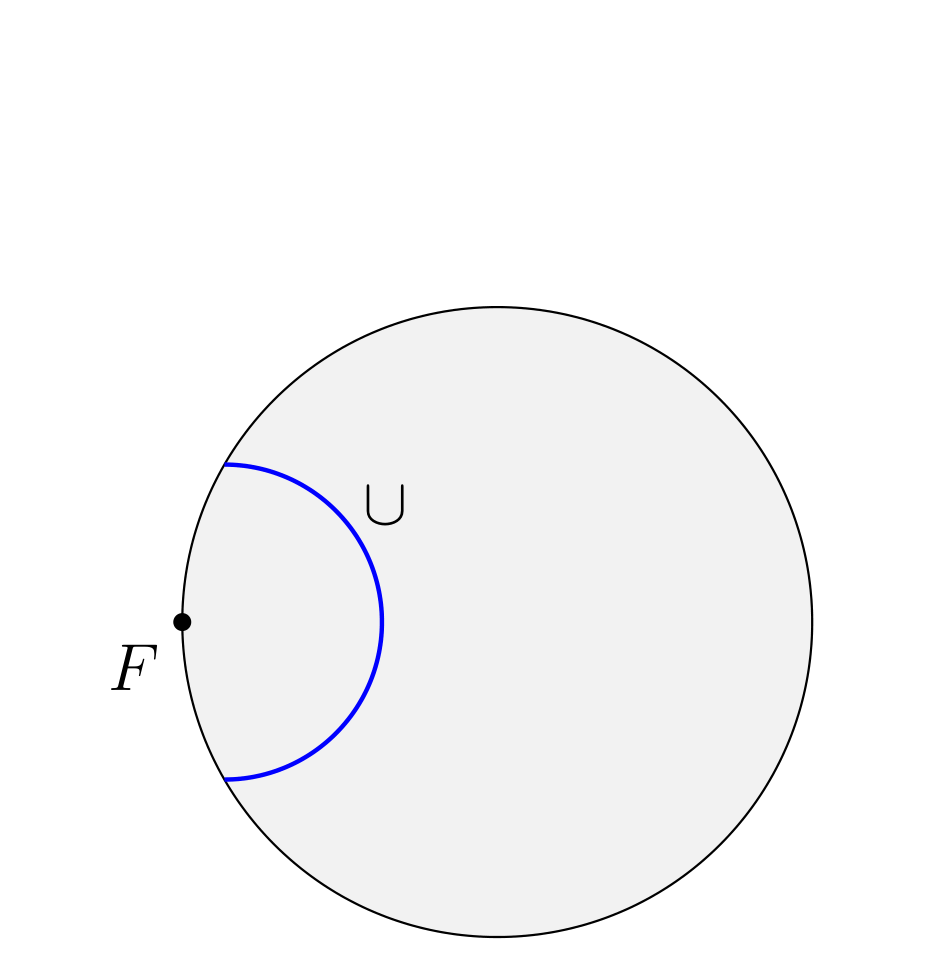
\includegraphics[width=0.40\textwidth]{figures/fig2_1.png}
\caption{cup 函子。}
\label{fig:cup-functor}
\end{figure}

\transnote{背景直觉：cup 函子把停点附近的小拉格朗日盘「绕过一圈」贴到纤维上，形状像把杯子扣在盘子上；cap 是它的形式伴随。}

cup 函子有形式伴随，它由左 Yoneda 模上的拉回 $\operatorname{Mod}\cW(X,F)\to\operatorname{Mod}\cW(F)$ 给出，我们称之为 \textbf{cap 函子}，记作 $\cap$。于是分别有余单位与单位态射 $\eps\colon\cup\cap\to\id$ 与 $\eta\colon\id\to\cap\cup$；把它们补全，就得到双模的正合三角形。这些正合三角形其实可以用 Seidel 早先的工作给出几何刻画：

\begin{thmstar}（Abouzaid--Ganatra, [AG]）\quad 存在双模的正合三角形
\[
\begin{tikzcd}[column sep=2.4em, row sep=1.5em]
\cup\cap \arrow[rr, "\varepsilon"] & & \id \arrow[dl] \\
& \sigma \arrow[ul, "+1"'] &
\end{tikzcd}
\]
（位于 $D^\pi\cW(X,F)$ 上）以及
\[
\begin{tikzcd}[column sep=2.4em, row sep=1.5em]
\cap\cup \arrow[dr, "+1"'] & & \id \arrow[ll, "\eta"] \\
& \mu \arrow[ur, "s"'] &
\end{tikzcd}
\]
（位于 $D^\pi\cW(F)$ 上），其中 $\mu\colon\cW(F)\to\cW(F)$ 是作用在纤维上的顺时针单值性，$\sigma\colon\cW(X,F)\to\cW(X,F)$ 是作用在全空间拉格朗日对象上的顺时针全扭转。此外，自然变换 $s$ 可以等同于 Seidel 的自然变换，后者首见于 [Sei09b]（另见 [Sei08a; Sei17]）。
\end{thmstar}

\transnote{易错预警：本论文第一部分取顺时针约定，与 [GPS20b] 的逆时针缠绕相容；读 [GPS20b] 时容易把 $\mu$ 的方向弄反，可对照 §2.3 的说明。}

本论文定理 \ref{thm:knorrer} 的证明在逻辑上并不需要这条定理；对后文的证明，读者可把 $\mu,\sigma,s$ 取为上文纯代数定义所给出的对象。其中一个三角形的证明梗概见 [AS15, Appendix]。

% ===== 原书 p.44 =====
两个三角形的约定并不相同：本论文第一部分采用的约定与 [GPS20b] 的逆时针缠绕相容，于是存在零次的自然变换 $\id\to\sigma$；这迫使 $\cup,\sigma,\mu$ 都取顺时针方向，且 $\cup$ 为左伴随。然而这样一来，在模型 Lefschetz 纤维丛的情形，$\mu$ 就是负的 Dehn twist 扭转。本论文第二部分则沿用 [Syl19c] 的约定：[Syl19d, Theorem 1.3] 证明，$f$ 绕 $\infty$ 的几何逆时针单值性 $\mu$ 作用在 $\cW(H)$ 上时，等于 $\cup$ 的对偶余扭转再平移 $[2]$；从而 $\mu$ 的镜像将是与线丛 $\cK_X^{-1}|_D$ 作张量。

\transnote{易错预警：在模型 Lefschetz 纤维丛情形，$\mu$ 是负的 Dehn twist 扭转；正负号取决于缠绕方向，不能与第二部分的约定混用。}

现在可以给出定义了：

\begin{defstar}（Auroux，复述第 1 章定义 \ref{def:sing-fuk}）\quad 设奇异辛纤维丛 $f\colon X\to\C$ 恰有一个奇异纤维，位于 $0$ 上方。则 $f^{-1}(0)$ 的 wrapped Fukaya 范畴定义为：在自然变换 $s\colon\mu\to\id$ 处，取 $t\neq0$ 充分小时的邻近纤维 $f^{-1}(t)$ 的 wrapped Fukaya 范畴的局部化：
\[
D\cW(f^{-1}(0))=D\cW(f^{-1}(t))[s^{-1}].
\]
\end{defstar}

\transnote{含糊点拨：原书把第 1 章的那条定义（定义 \ref{def:sing-fuk}）原样复述，编号也保持不变。此处的译文按引用式复述处理，不占本章编号。}

条件“$|t|\neq0$ 充分小”是为了排除 $t$ 是 Malgrange 条件失效点的可能；§2 前面的定义已把这类点排除在 Landau--Ginzburg 模型之外。

% ===== 原书 p.45 =====
注意，这一定义等价于对范畴 $\cW(f^{-1}(t))$ 取商，商掉由该自然变换的各锥构成的满子范畴；也就是说，商掉复合 $\cap\cup$ 的本质像。下面这条引理在计算中常常有用：

\begin{lemma}\label{lem:essential-image}\label{lem:2-3-1}
复合 $\cap\cup$ 的本质像与 $\cap$ 的本质像有相同的分裂闭包。
\end{lemma}

\begin{proof}
一个包含关系是显然的。为证反向包含，考虑联系 $\cap$ 与 $\cup$ 之复合的两个正合三角形；须注意，按上面的约定，这两个三角形的箭头方向相反，其中 $\eps$ 与 $\eta$ 分别是 $\cup$--$\cap$ 伴随的余单位与单位。我们对第一个三角形作用 $\cap$，并在第二个三角形前复合 $\cap$。由正合性以及恒等式 $\mu\cap=\cap\sigma$ [AG]，得到两个三角形：
\[
\begin{tikzcd}[column sep=3.2em, row sep=1.5em]
\cap\cup\cap \arrow[rr, "\cap\varepsilon"] & & \cap \arrow[dl] \\
& \mu\cap \arrow[ul, "+1"'] &
\end{tikzcd}
\]
\[
\begin{tikzcd}[column sep=3.2em, row sep=1.5em]
\cap\cup\cap \arrow[dr, "+1"'] & & \cap \arrow[ll, "\eta\cap"] \\
& \mu\cap \arrow[ur] &
\end{tikzcd}
\]
伴随的单位–余单位恒等式 $\cap\eps\circ\eta\cap=\id_{\cap}$ 说明第二个三角形中的映射 $\mu\cap\to\cap$ 为零，故该三角形分裂。于是 $\cap\cup\cap L$ 总以 $\cap L$ 为直和项。
\end{proof}

\transnote{易错预警：两个三角形的箭头方向相反；须先对第一个作用 $\cap$，再给第二个前复合 $\cap$，顺序颠倒会得到不同的三角形。}

% ===== 原书 p.46 =====
\begin{figure}[htbp]
\centering
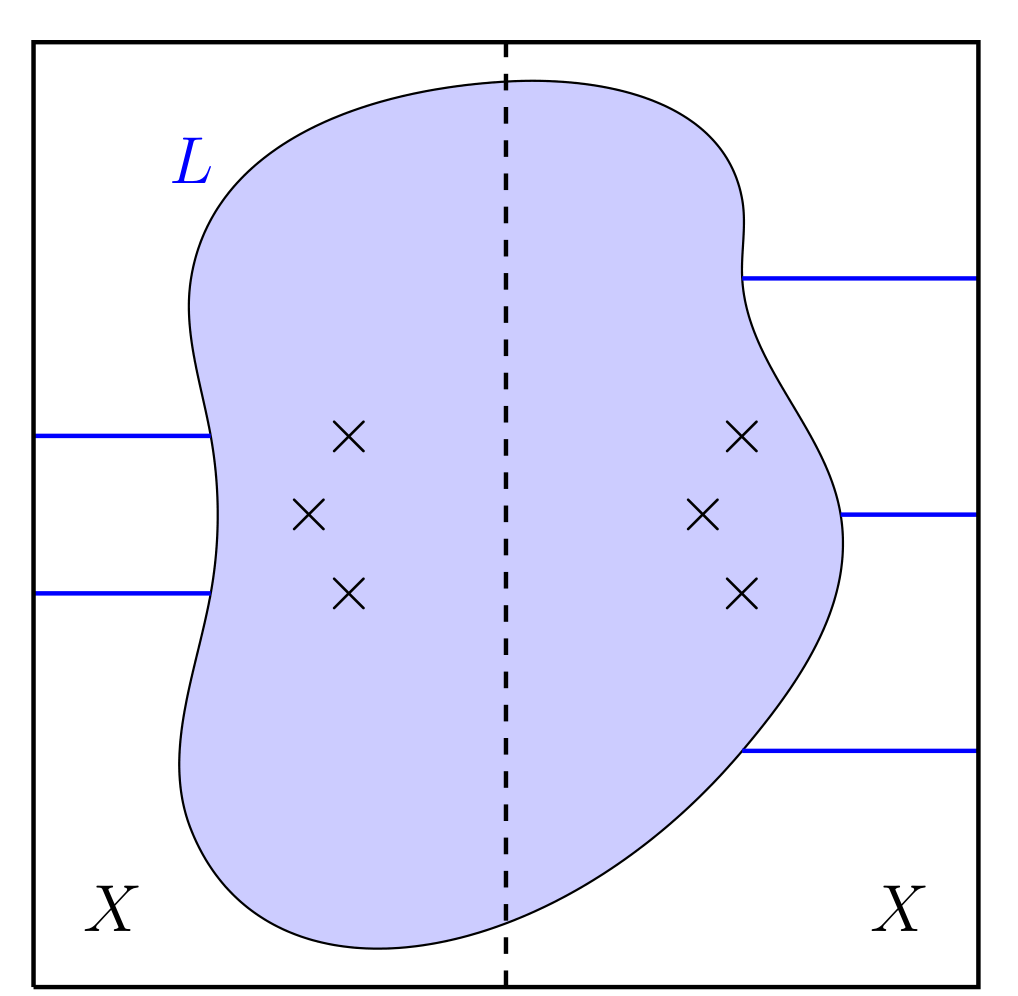
\includegraphics[width=0.52\textwidth]{figures/fig2_2.png}
\caption{拼接起来的若干份 $X$ 内部的拉格朗日配边 $L$。}
\label{fig:cobordism}
\end{figure}

\begin{remarkx}\label{rem:7}
要看出定理 \ref{thm:knorrer} 中取扭复形的分裂闭包是必要的，可考虑如下情形：绕奇异纤维的单值性由绕同一 vanishing cycle 的两个 Dehn twist 扭转之复合给出。
\end{remarkx}

\transnote{背景直觉：取分裂闭包是为让锥在幂等分裂下封闭；绕同一消失圈复合两次 Dehn twist 扭转时，缺了它范畴就会漏掉直和项。}

\begin{corollary}\label{cor:sing-fuk-quotient}\label{cor:2-3-2}
范畴 $D^\pi\cW(f^{-1}(0))$ 拟等价于 $D^\pi\cW(f^{-1}(t))$ 商掉 $\cap$ 的本质像所得的商范畴。
\end{corollary}

\begin{proof}
由引理 \ref{lem:essential-image}，函子 $\cap\cup$ 与 $\cap$ 的本质像有相同的分裂闭包，因此所得的两个商范畴彼此拟等价。
\end{proof}

若读者希望避开 [AG]，也可在证明定理 \ref{thm:knorrer} 时改把推论 \ref{cor:sing-fuk-quotient} 当作定义。

定义 \ref{def:sing-fuk} 与辛纤维丛内部的拉格朗日配边还有一层特别自然的关系（参看 [BC17]）。代替研究乘积 $f^{-1}(t)\times\C$ 中的拉格朗日配边，我们可以改为考虑 $X$ 内部（或若干个 $X$ 拼接起来）的拉格朗日配边，只要求其两端经 $f$ 投影到与正实轴或负实轴平行的射线上：见图 \ref{fig:cobordism}。在作一次哈密顿同痕之后，每条这样的配边都可以只看作只有正端；于是这些零配边给出了拉格朗日配边群上全部的关系。而这些关系说的正是：$\cap$ 的像中的每个复形都必须等价于零。由推论 \ref{cor:sing-fuk-quotient}，这正是深谷范畴 $\cW(f^{-1}(0))$ 的等价描述。因此我们猜想，这一构造刻画了 Grothendieck 群 $K_0(D^\pi\cW(f^{-1}(0)))$。

\transnote{含糊点拨：原文此处是 conjecture，作者并未证明，引用时不可当作定理；它把配边群与 $K_0$ 联系起来。}
% ===== 原书 p.47 =====

\clearpage
% EN49 c05 | 原书 p.48–57（PDF 59–68） | 第 3 章（无小节）
\section{纤维的补集}

% ===== 原书 p.48 =====
本章先记录若干简单观察，主题是 Landau--Ginzburg 模型 $(X\times\C,\,z(f-t))$ 随 $t$ 变化的几何。
本节约定 $f_t(z)=f(z)-t$。

首先注意，$z(f-t)$ 只有一个临界纤维，出现在 $z(f-t)=0$ 处。
该纤维作为集合由 $(f^{-1}(t)\times\C)\cup(X\times\{0\})$ 给出；临界轨迹恰为 $f^{-1}(t)$。
注意当 $t\ne0$ 时，该临界轨迹因而光滑，我们得到显式的局部 Morse--Bott 模型，细节见下。

对 $\eps\ne0$，$z(f-t)$ 在 $\eps$ 上方的光滑纤维为
\[
  \{(x,z): f(x)\ne t,\ z=\eps/f_t\},
\]
作为集合可等同于补集 $X\setminus f^{-1}(t)$。
该补集上相应的 Liouville 结构来自 Stein 函数到纤维的限制。

\transnote{易错预警：临界纤维作为集合是 $(f^{-1}(t)\times\C)\cup(X\times\{0\})$，比临界轨迹 $f^{-1}(t)$ 大一圈。$X\times\{0\}$ 那部分不是临界点，只在集合层面属于奇异纤维，勿把它算进临界轨迹。}

% ===== 原书 p.49 =====
利用因子 $\C$ 上的 Stein 函数 $|z|^{2n}$，这一结构由
\[
  \psi(x)=\phi(x)+\frac{\eps^{2n}}{|f_t(x)|^{2n}}
\]
给出。该 Stein 函数也可这样得到：取 $X\setminus f^{-1}(t)$ 到 $\C^{N+1}$ 的嵌入
$x\mapsto(i(x),\eps/f_t(x))$。

\transnote{易错预警：$\eps$ 是 $\C$ 方向上的取值，不是形变参数。$z=\eps/f_t$ 自带 $1/z$ 型行为，故 $\psi$ 中出现的是 $|f_t|^{-2n}$ 而不是 $|f_t|^{2n}$；指数取反就换成了另一个 Stein 结构。}

我们改用补集上一个形变等价的 Stein 结构，它由
\[
  \psi(x)=\phi(x)+\frac{C\phi(x)}{|f_t(x)|^{2n}}
\]
给出，其中 $C>0$ 与 $n\in\N$ 取合适的值。
该 Stein 函数来自 $X\setminus f^{-1}(t)$ 到 $\C^{2N}$ 的嵌入
$x\mapsto(i(x),\sqrt{C}\,i(x)/f_t(x)^n)$，并与前一结构 Stein 形变等价；形变为
\[
  \psi_s(x)=\phi(x)+\frac{s+\phi(x)}{1+s\phi(x)}\frac{C}{|f_t(x)|^{2n}},
  \qquad s\in[0,1].
\]

\transnote{含糊点拨：两处「Stein 结构」并不相同，但只差一个 Stein 形变。按引理 \ref{lem:simple-homotopy}，形变只改变 Liouville 结构、不改 wrapped Fukaya 范畴的拟等价类，故后面可以随意换用。}

要理解 $t\ne0$ 与 $t=0$ 时 $(X\times\C,z(f-t))$ 的 LG 模型如何不同，需要研究一般纤维的 Liouville 结构如何变化。
下面这个初等例子说明了做法。

\begin{example}\label{exam:3-0-1}
我们回忆如何在 Lefschetz 纤维丛上构造标准 Weinstein 结构。
考虑标准 Lefschetz 纤维丛 $f\colon\C^2\to\C$，并给 $\C^2$ 配标准 Stein 结构。
考察纤维 $f^{-1}(t)$ 的补集的骨架。
当 $t=0$ 时，$\C^2\setminus f^{-1}(0)=(\C^*)^2$ 带标准 Liouville 结构，故其骨架对应于零截面 $T^2\subseteq T^*T^2\cong(\C^*)^2$。

% ===== 原书 p.50 =====
\begin{figure}[htbp]
  \centering
  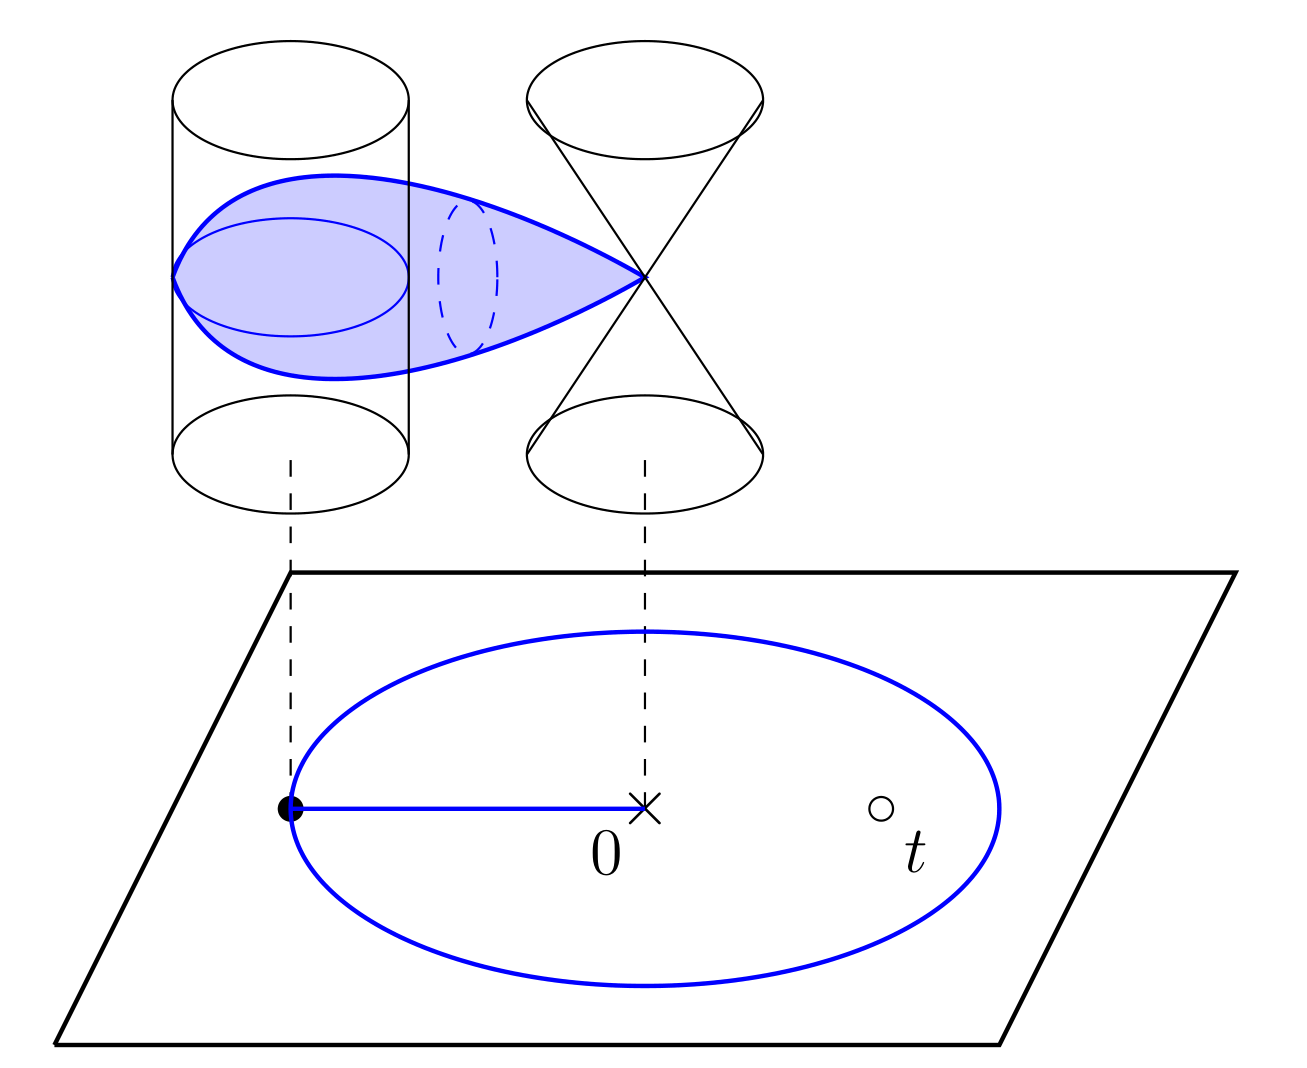
\includegraphics[width=0.42\textwidth]{figures/fig3_1.png}
  \caption{例 \ref{exam:3-0-1} 中的骨架（蓝色）。}
  \label{fig:3-1}
\end{figure}

注意，$\C^2$ 上 Stein 结构给出的 Weinstein 函数在 $0$ 处只有一个临界点，指标为 $2$。
取 $t\ne0$ 后，$X\setminus f^{-1}(t)$ 上的 Weinstein 函数现在包含这个临界点。
因此 $\C^2\setminus f^{-1}(t)$ 由 $\C^2\setminus f^{-1}(0)$ 附加一个临界 Weinstein 把手得到。
$\C^2\setminus f^{-1}(t)$ 的骨架现在包含该把手的核，它附着在原来的 $T^2$ 上，见图 \ref{fig:3-1}。\hfill$\Box$
\end{example}

\transnote{背景直觉：例子说明的是「挖掉的纤维从 $0$ 移到 $t$」这一动作。$t\ne0$ 时 $0$ 处那个临界点落进了补集，于是补集相当于在 $T^2$ 上粘了一个把手；命题 \ref{prop:3-0-3} 把这幅图景推广到一般 $X$。}

为描述一般情形，我们需要引理 \ref{lem:local-psi-outward} 的对偶版本。

\begin{proposition}\label{prop:3-0-2}
  对充分大的 $C>0$、$n\in\N$ 以及充分小的 $t$，$\psi$ 的 Liouville 向量场在 $\{|f_t|^2=\delta\}$ 上内指，
  对一切充分小的 $\delta>0$ 成立。
\end{proposition}

\begin{proof}
考察内积
\[
  \langle\nabla_X|f_t|^2,\nabla_X\psi\rangle
  =\Bigl(1+\frac{C}{|f_t|^{2n}}\Bigr)\langle\nabla_X|f_t|^2,\nabla_X\phi\rangle
  -\frac{nC\phi}{|f_t|^{2n+2}}|\nabla_X|f_t|^2|^2 .
\]

% ===== 原书 p.51 =====
由 Cauchy--Schwarz 不等式，只要
\[
  2\Bigl(\frac{|f_t|^{2n+2}}{C}+|f_t|^2\Bigr)
  <n|\phi|^{1/2}|\nabla_X|f_t|^2|,
\]
在 $|f_t|^{-1}(\delta)$ 上就有 $\langle\nabla_X|f_t|^2,\nabla_X\psi\rangle<0$。
再次取 $|t|,\delta>0$ 充分小，可保证对某个充分大的 $n\in\N$，Malgrange 条件在 $|f_t|^2=\delta$ 上成立，命题得证。
\end{proof}

\transnote{易错预警：命题 \ref{prop:3-0-2} 是引理 \ref{lem:local-psi-outward} 的对偶，结论却是「内指」。差别出在负指数上：$\nabla_X|f_t|^{-2n}$ 带出因子 $-2n|f_t|^{-2n-1}$，故末项为 $-\dfrac{nC\phi}{|f_t|^{2n+2}}|\nabla_X|f_t|^2|^2$，符号与引理 \ref{lem:local-psi-outward} 的正指数项相反。}

\begin{remarkx}\label{rem:8}
注意可以把上述论证中的 $\phi$ 换成与引理 \ref{lem:local-psi-outward} 的 Stein 函数同伦的 Stein 函数
\[
  \psi=\phi+C\phi|f_t|^{2m},
\]
从而让引理 \ref{lem:local-psi-outward} 与命题 \ref{prop:3-0-2} 同时成立（在同心的圆盘上）。所得不等式
\[
  C|f_t|^2+|f_t|^{2n+2}+D|f_t|^{2m+2n+2}
  <\frac{\phi^{1/2}}{2}|\nabla_X|f_t|^2|\bigl(Cn-Dm|f_t|^{2m+2n}\bigr)
\]
在 $\eps\le|f_t|^2\le\delta$ 上成立，其中 $\delta>\eps>0$ 充分小，$C,n$ 在给定 $D,m$ 后取得充分大。
\end{remarkx}

\transnote{含糊点拨：本条不等式给出两套构造同时成立的充分条件，不是新的估计。右端括号 $Cn-Dm|f_t|^{2m+2n}$ 须为正，这就是先取 $C,n$、再取 $D,m$ 的顺序不能颠倒的原因。}

现在我们用 Eliashberg 的 Weinstein 流形手术理论，来理解一般纤维随 $t$ 的变化：

\begin{proposition}\label{prop:3-0-3}
  上述 $X\setminus f^{-1}(t)$ 上的 Weinstein 结构，由 $X\setminus f^{-1}(0)$ 附加一族 Weinstein 把手得到。
\end{proposition}

% ===== 原书 p.52 =====
\begin{proof}
先说明如何从 $X\setminus f^{-1}(0)$ 过渡到 $X\setminus f^{-1}(B_\delta)$，两者都配 Stein 函数
\[
  \psi_0(x)=\phi(x)+\frac{C\phi(x)}{|f(x)|^{2n}}.
\]
由命题 \ref{prop:3-0-2}，对充分小的 $\delta>0$ 与充分大的 $n,C$，可取 $B_\delta$ 为 $0$ 处的球，
使 $\psi_0$ 在 $X$ 上的 Liouville 向量场沿 $|f|^{-1}(\delta)$ 内指。
再把 $\delta>0$ 缩小，可使 $f^{-1}(B_\delta\setminus\{0\})$ 中没有该 Liouville 向量场的零点，
因为 $\phi$ 在 $X$ 上的零点在映射 $f\colon X\to\C$ 下是孤立的。
于是 $X\setminus f^{-1}(0)$ 与 $X\setminus f^{-1}(B_\delta)$ 之间有一个平凡的 Weinstein 配边，
因而有 Liouville 流形的同构 [CE12]。

取 $|t|<\delta$，现在从 $X\setminus f^{-1}(B_\delta)$ 过渡到 $X\setminus f^{-1}(t)$。
首先，$X\setminus f^{-1}(B_\delta(s))$ 上有一族 Weinstein 结构形变（对 $|s|<\delta$ 都微分同胚）：
\[
  \psi_s(x)=\phi(x)+\frac{C\phi(x)}{|f_s(x)|^{2n}},\qquad s\in[0,t].
\]
对充分小的 $\eps>0$，$\psi_s$ 在 $f^{-1}(B_\delta)$ 之外的临界点当 $s$ 从 $0$ 变到 $t$ 时都不进入 $f^{-1}(B_\delta(s))$：
故这是简单 Liouville 形变，于是 $\psi_0$ 与 $\psi_t$ 在 $X\setminus f^{-1}(B_\delta)$ 与 $X\setminus f^{-1}(B_\delta(t))$ 上给出同构的 Liouville 结构（引理 \ref{lem:simple-homotopy}）。

现在，由于 $\psi_t$ 的 Liouville 向量场沿 $f^{-1}(\partial B_\delta)$ 内指，
注意 $f^{-1}(B_\delta)\setminus f^{-1}(t)$ 给出从 $X\setminus f^{-1}(B_\delta)$ 到 $X\setminus f^{-1}(t)$ 的 Weinstein 配边。
于是由 Eliashberg 的 Weinstein 流形手术理论 [CE12]，沿 $X\setminus f^{-1}(B_\delta)$ 的边界附加

% ===== 原书 p.53 =====
\begin{figure}[htbp]
  \centering
  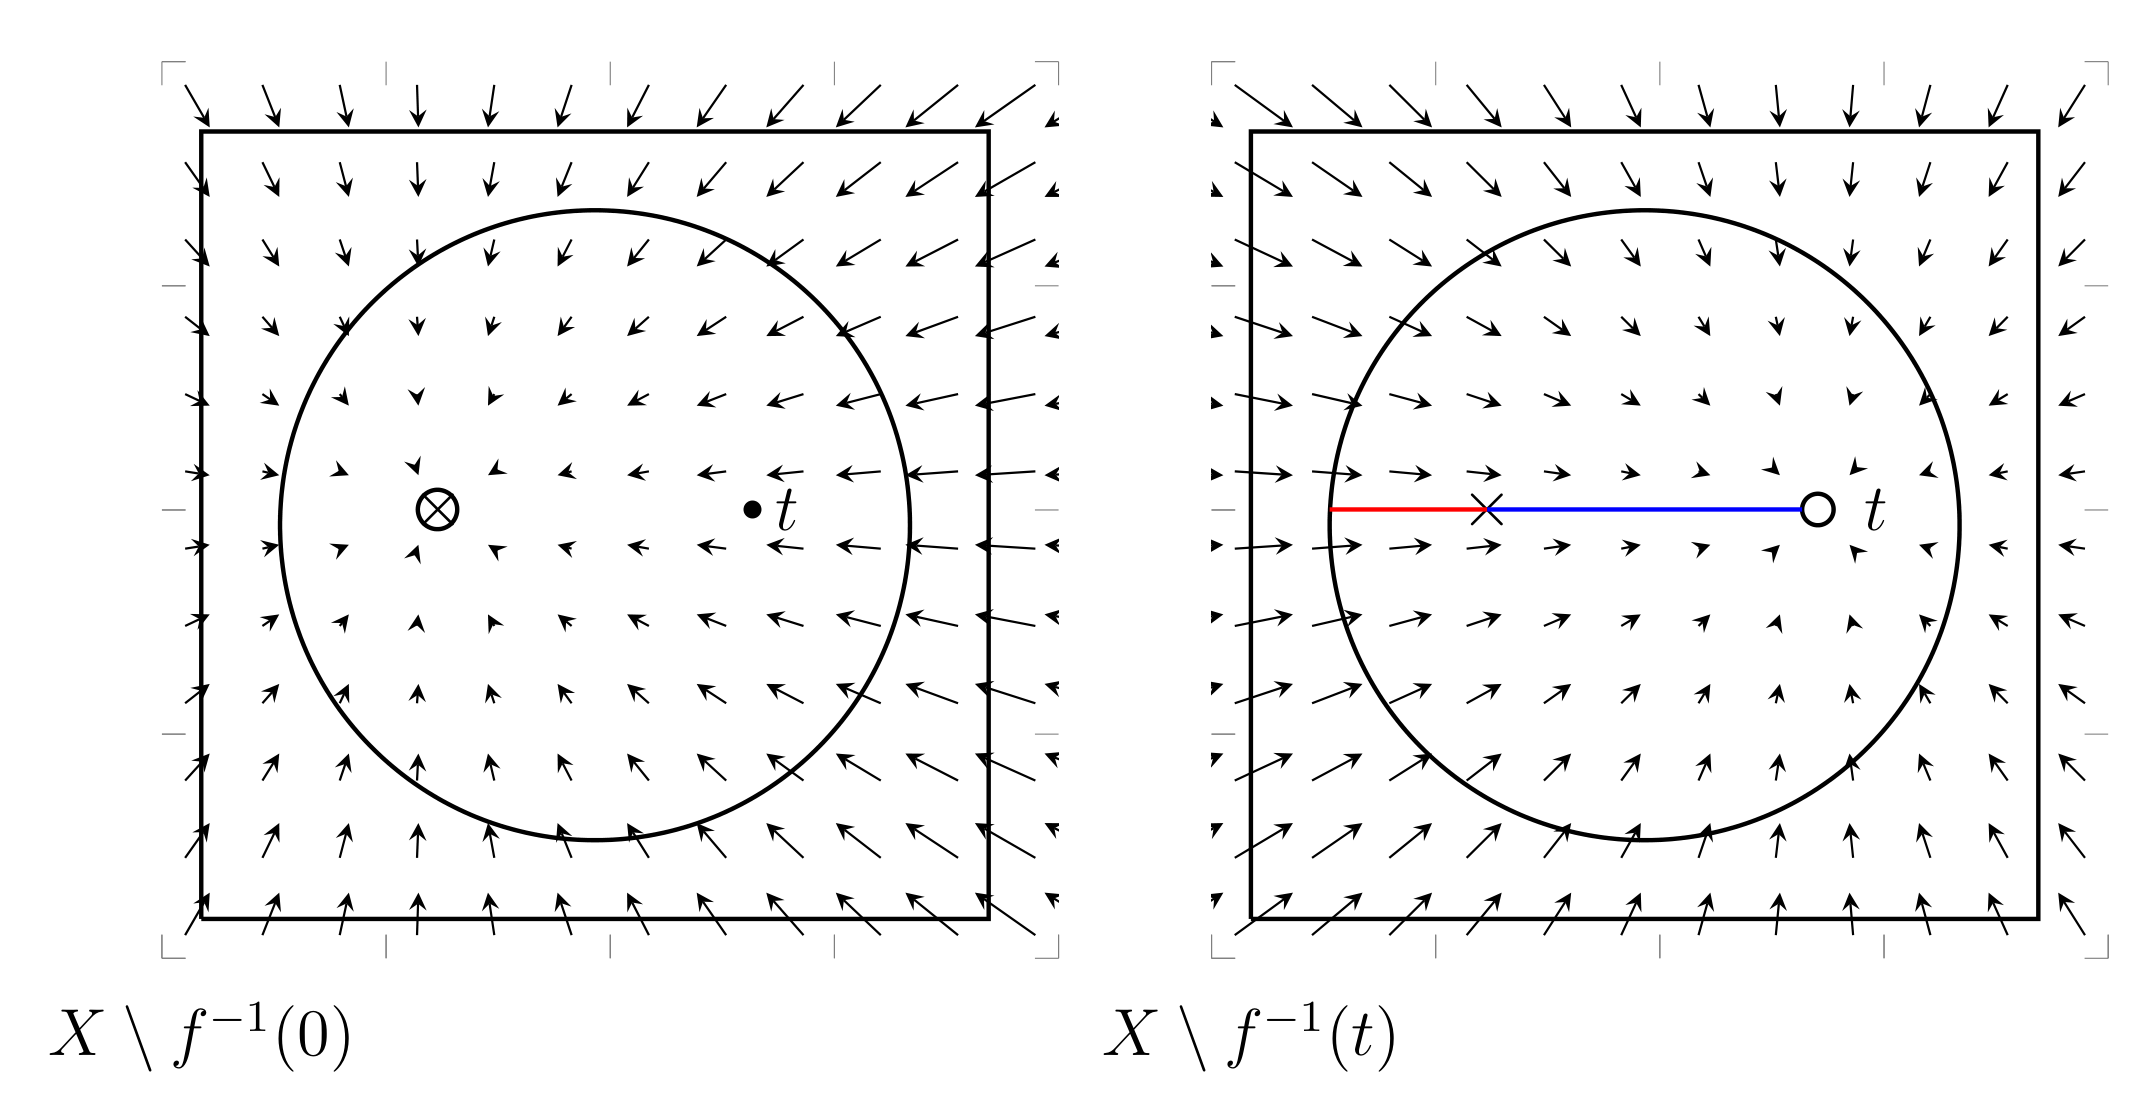
\includegraphics[width=0.86\textwidth]{figures/fig3_2.png}
  \caption{命题 \ref{prop:3-0-3} 的把手附加过程：新增把手的核为红色，余核为蓝色。}
  \label{fig:3-2}
\end{figure}

Weinstein 把手，即得 $X\setminus f^{-1}(t)$：见图 \ref{fig:3-2}。
\end{proof}

命题 \ref{prop:3-0-3} 给出的临界把手统称为\textbf{附加把手}（additional handles）。
应用 Ganatra--Pardon--Shende 的去停点定理 [GPS19, Theorem 1.16]，我们得到：

\begin{proposition}\label{prop:3-0-4}
  取上述构造的 Liouville 结构，则有范畴等价
  \[
    \cW(X\times\C,zf)\cong\cW\bigl(X\times\C,z(f-t)\bigr)/\cD,
  \]
  其中 $\cD$ 是 $\cW(X\times\C,z(f-t))$ 的满子范畴，由 $X\setminus f^{-1}(t)$ 中附加把手的稳定流形的环绕圆盘张成。
\end{proposition}

\transnote{易错预警：命题 \ref{prop:3-0-4} 的商是「满子范畴 $\cD$ 的商」，不是对理想或对对象取商。$\cD$ 由附加把手稳定流形的环绕圆盘张成，与命题 \ref{prop:3-0-5} 的余核是同一批几何对象的两个侧面。}

\begin{proposition}\label{prop:3-0-5}
  对上述 Stein 流形 $X$ 上的函数 $f$，范畴 $\cW(X,f)$ 由附加把手的余核分裂生成。
\end{proposition}

% ===== 原书 p.54 =====
证明中我们会说明附加把手的余核（记作 $\ell_i$）在什么意义下是 $\cW(X,f)$ 的对象。

\begin{proof}
先研究 $X\setminus f^{-1}(B_\delta)$ 的 wrapped Fukaya 范畴，其 Stein 结构为
\[
  \psi(x)=\phi(x)+\frac{C\phi(x)}{|f(x)|^{2n}},
\]
其中 $\delta,C,n$ 如命题 \ref{prop:3-0-3} 的证明中所取。
如注 \ref{rem:8} 那样，通过改变 $\phi$ 可得某个 $R>\delta$，使 $\psi$ 的 Liouville 向量场沿 $|f|^{-1}(R)$ 也外指。
为此我们想如下加入停点：
\begin{itemize}
  \item 停点 $F$，由 $f^{-1}(-R)$ 给出；
  \item $|f|^{-1}(\delta)$ 上的停点 $\Lambda$，由附加把手 $\ell_i$ 所沿附着的带标架 Legendrian 球面 $\Lambda_i$ 给出。
\end{itemize}
由生成性结果 [GPS19, Theorem 1.10]，$\cW(X\setminus f^{-1}(B_\delta),F\cup\Lambda)$ 由两类拉格朗日对象生成：
\begin{itemize}
  \item $F$ 与 $\Lambda_i$ 的环绕圆盘；
  \item 由 $f^{-1}(t)$ 的余核与连接 $-R$ 到 $|f|^{-1}(\delta)$ 的弧 $\gamma$ 的乘积给出的拉格朗日对象 $L$。
\end{itemize}
用 [GPS19, Theorem 1.9] 的缠绕正合三角形，可以把 $F$ 的环绕圆盘用 $L$ 与 $\Lambda_i$ 的环绕圆盘的扭复形表示，如图 \ref{fig:3-3}。
注意取乘积所用的弧 $\gamma$ 在复平面中位于停点 $F,\Lambda$ 之下。

% ===== 原书 p.55 =====
\begin{figure}[htbp]
  \centering
  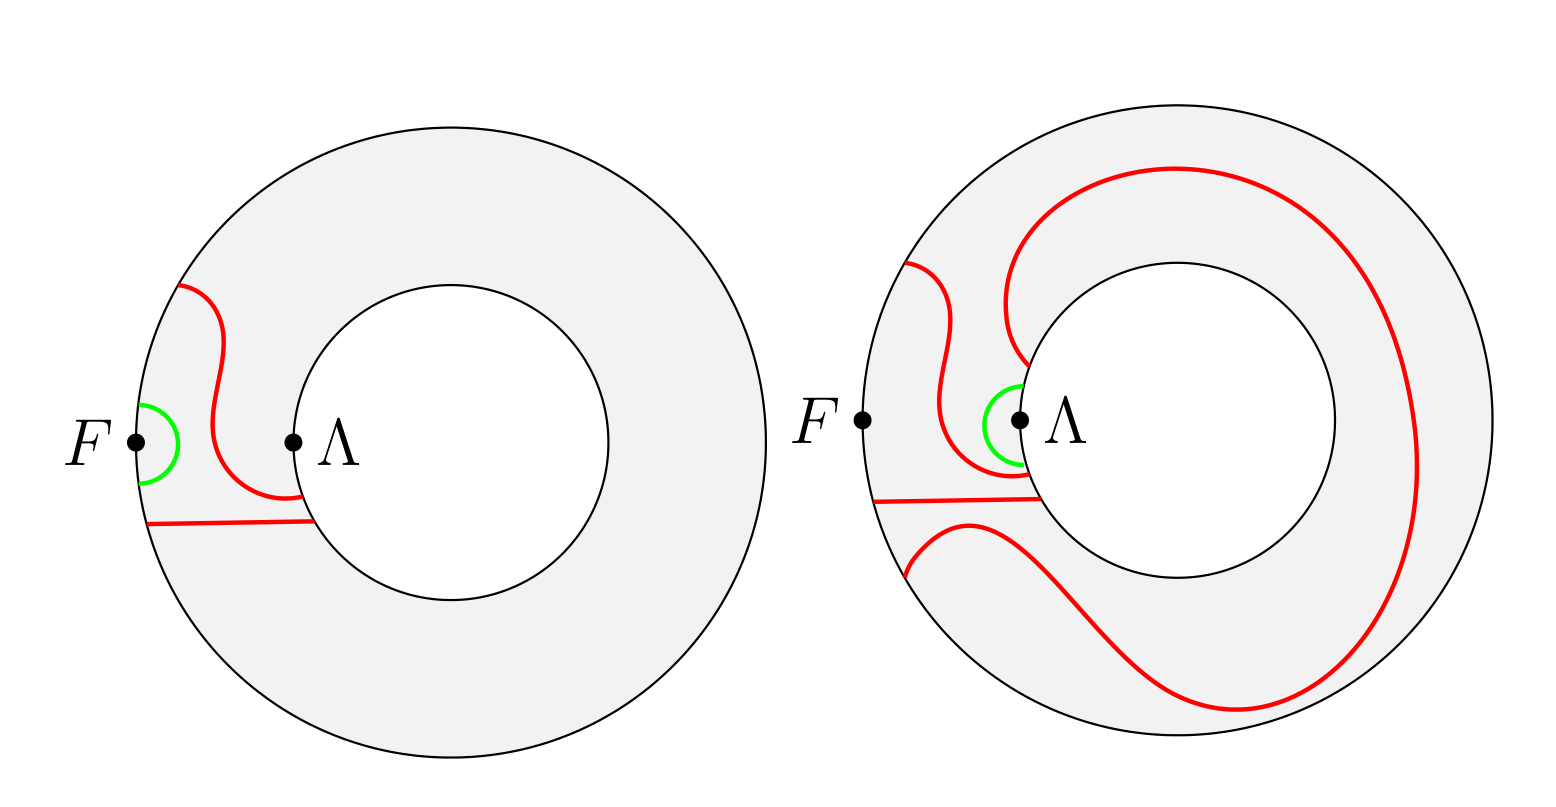
\includegraphics[width=0.78\textwidth]{figures/fig3_3.png}
  \caption{由对象 $L$（红色）与 $\Lambda$ 的环绕圆盘（绿色）造出 $F$ 的环绕圆盘。}
  \label{fig:3-3}
\end{figure}

\transnote{易错预警：图中弧 $\gamma$ 必须画在停点 $F,\Lambda$ 之下。缠绕正合三角形的符号与「上下」约定绑定，画反了会得到相反的同调移位。}

现在依命题 \ref{prop:3-0-3} 附加 Weinstein 把手，过渡到 $(X\setminus f^{-1}(t),f)$，同时保持 Liouville 向量场沿 $|f|^{-1}(R)$ 外指。
此时 $\Lambda_i$ 的环绕圆盘恰好变成附加把手的余核 $\ell_i$，
于是由 [GPS19, Theorem 1.20] 的粘合结果知，$\cW(X\setminus f^{-1}(t),f)$ 由附加余核 $\ell_i$ 与拉格朗日对象 $L$ 生成（参看 [GPS19, p.68]）。
可以把这些 $L$ 取为在从 $-R$ 到 $f^{-1}(t)$ 的弧 $\gamma$ 上纤维化、且经过 $f$ 的奇异纤维之下、停点 $F$ 之下的对象。

现在考虑 Weinstein 形变
\[
  \psi_t(x)=\phi(x)+\frac{C\phi(x)}{|f_t(x)|^{2n}}.
\]
与注 \ref{rem:8} 类似地论证：对一切充分小的 $\eps>0$，可选 $\phi$、更大的 $C,n$ 与更小的 $R,\delta$，
使得存在某个 $R'>R+\eps$，满足 $|f|^2$ 的 Malgrange 条件失效的所有点都落在 $|f|\le R'+\eps$ 之外，并且
\begin{itemize}
  \item 当 $0<|t|<R+\eps$ 时，$\psi_t$ 在 $X\setminus f^{-1}(t)$ 上的 Liouville 向量场沿 $|f|^{-1}(r)$ 外指，其中 $R'+\eps>r\ge R'$；

% ===== 原书 p.56 =====
  \item 当 $R+\eps/2<|t|<R+\eps$ 时，该 Liouville 向量场沿 $|f|^{-1}(R)$ 外指。
\end{itemize}

第一个性质防止 Liouville 域的骨架逃出某个紧集之外，
故 $\psi_t$ 给出 $X\setminus f^{-1}(t)$ 在 $0<|t|<R+\eps$ 时的简单 Weinstein 形变。
于是所得的 $X\setminus f^{-1}(t)$ 彼此正合辛同胚，wrapped Fukaya 范畴 $\cW(X\setminus f^{-1}(t),f)$ 保持不变（引理 \ref{lem:simple-homotopy}）。

$\psi_t$ 在 $R+\eps/2<|t|<R+\eps$ 时的第二个性质意味着：由于停点 $F$ 位于 $|f|^{-1}(-R)$ 之内，
我们得到 $(X\setminus f^{-1}(t),f)$ 的一个子扇形 $(f^{-1}(B_R(0)),f)$；见图 \ref{fig:3-4}。
应用 Viterbo 限制，对象 $L$ 与 $\ell_i$ 分裂生成 $\cW(f^{-1}(B_R(0)),f)$（由 [Syl19c, Theorem 1.8]）。
但 $(f^{-1}(B_R(0)),f)$ 与 \S2 中用于定义 $\cW(X,f)$ 的原始扇形 Weinstein 形变等价，形变为
\[
  \psi_{t,s}(x)=\phi(x)+C\phi(x)\rho_s(f_t(x))
\]
其中 $s\in(0,1]$，$\rho_s(z)=\beta_s(|z|)/|z|^{2n}$，$\beta_s\colon\R\to[0,1]$ 是光滑截断函数，取法满足
\[
  \beta_s(r)=
  \begin{cases}
    1 & \text{当 } r\le\tan(\pi s/2),\\
    0 & \text{当 } r\ge\tan(\pi s/2)+\eps,
  \end{cases}
\]
并使 $\rho_s(f_t(x))$ 多重次调和（这里 $\psi_1=\psi$）。
此外，对一切 $s\in(0,1]$，$\psi_{t,s}$ 的 Liouville 向量场在 $R+\eps>|t|>r\ge R+\eps/2$ 时沿 $|f|^{-1}(r)$ 保持外指，故这实际上给出简单 Weinstein 形变。

\transnote{背景直觉：Viterbo 限制把整体范畴的生成元压到子扇形上，这一步是「先局部生成、再回到整体」的枢纽。子扇形只保留 $|f|\le R$ 的部分，故 $\beta_s$ 必须把 $f_t$ 截断在 $R$ 附近，同时保持多重次调和性。}

% ===== 原书 p.57 =====
\begin{figure}[htbp]
  \centering
  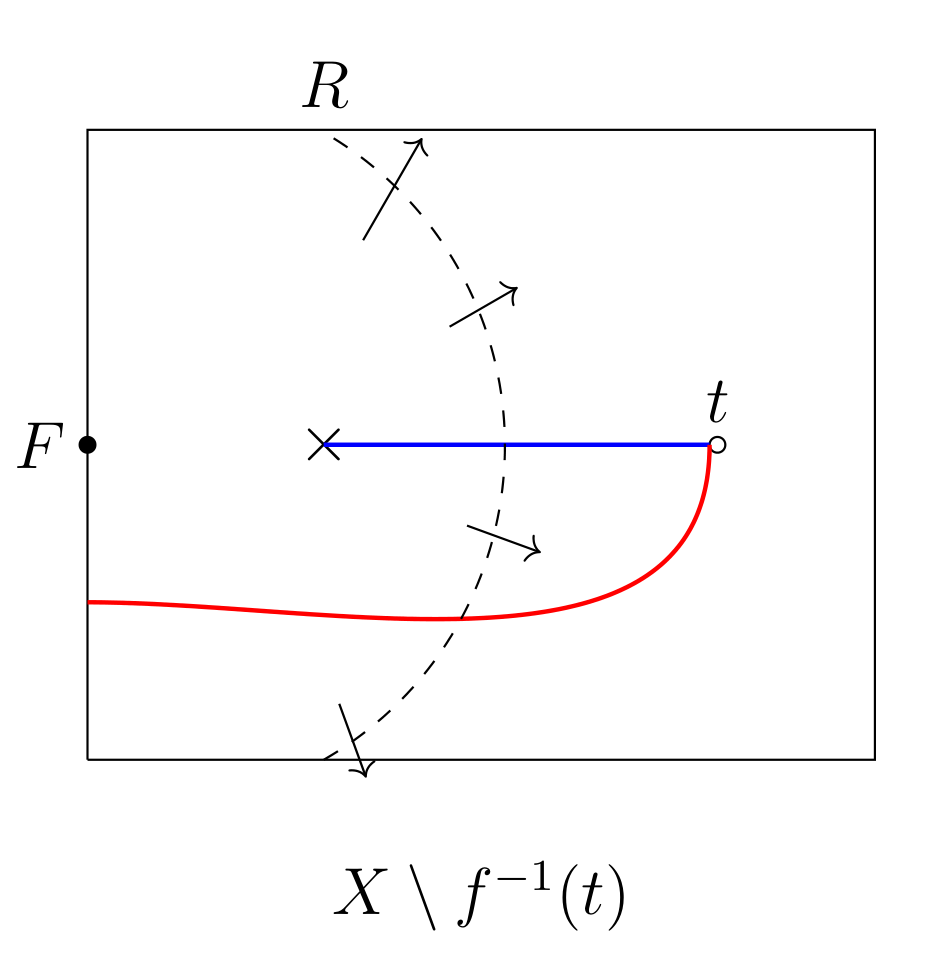
\includegraphics[width=0.36\textwidth]{figures/fig3_4.png}
  \caption{命题 \ref{prop:3-0-5} 中构造的子区域：对象 $L$ 为红色，余核 $\ell_i$ 为蓝色。}
  \label{fig:3-4}
\end{figure}

于是我们得到 $\cW(X,f)$ 的分裂生成元 $L$ 与 $\ell_i$（引理 \ref{lem:simple-homotopy}）。
但前者在该范畴中是平凡的，因为它们可经哈密顿推移到无穷远而与自身错开。
于是得到所要的分裂生成结论。
\end{proof}

\transnote{背景直觉：整个证明是「先在大空间里生成，再限制到子扇形，最后把多余生成元杀掉」。$L$ 在 $\cW(X,f)$ 中平凡，是因为它可被哈密顿推到无穷远，这一点正是「只有余核 $\ell_i$ 真正参与生成」的几何来源。}

\clearpage
% EN49 c06 | 原书 原书 p.58–64（PDF 69–75） | 第 4 章 §4.1
% 骨架文件：标题行已设定，正文由译者填写。每页起首用 % ===== 原书 p.N ===== 注释标记。
\section{超曲面的 Kn{\"o}rrer 周期性}

\subsection{AAK 等价}

% ===== 原书 p.58 =====
我们先证明超曲面情形的光滑 Kn{\"o}rrer 周期性，即定理 \ref{thm:aak-equiv}（Abouzaid--Auroux--Katzarkov 等价）：

\begin{thmstar}
设 $X$ 是光滑仿射簇，带嵌入 $X\to\C^N$，该嵌入在 $X$ 上诱导 Stein 结构；设
$f\colon X\to\C$ 是 $\C^N$ 上多项式函数的限制。若 $f$ 只有一个临界纤维
$f^{-1}(0)$，则对充分小的 $t\neq0$，存在 $A_\infty$ 范畴的拟等价
\[
T\colon\cW(f^{-1}(t))\to\cW(X\times\C,z(f-t)),
\]
\end{thmstar}

\transnote{易错预警：原书在第 4 章开头把引言中的定理 \ref{thm:aak-equiv} 原样重述，并沿用原编号。
译本编号全部自动生成，若另立有编号的定理环境，同一结论会得到「4.1.1」的新号，还会把
紧随其后的那条定义挤成下一号。故此处用无编号的 thmstar 环境，编号一律引
定理 \ref{thm:aak-equiv}。后文重述定理 \ref{thm:relative}、\ref{thm:knorrer} 同此处理。}

% ===== 原书 p.59 =====
该函子由在奇异轨迹 $f^{-1}(t)$ 中的可容拉格朗日子流形上取顶针给出。

首先，我们要描述证明中将在 $(X\times\C,z(f-t))$ 上使用的 Liouville 结构与近复结构
（almost-complex structure）。
以下记 $F_t=z(f-t)$。这里想提醒读者注意注 \ref{rem:6} 中的约定，即如何为
Landau--Ginzburg 模型的单个临界值构造局部 Liouville 扇形。

\transnote{含糊点拨：原书此处只写「Remark 6」，未带节号，页图上该编号也不是红色链接；
它应指第 2 章里按独立序列编号的第 6 条注，但底本没有给出更精确的定位。译本按第 2 章的
注记编号引作「注 6」，正文照译，不补猜测。}

首先，由命题 \ref{prop:2-2-6}，因 $t\neq0$ 时 $f^{-1}(t)$ 光滑，我们可以把
$V=f^{-1}(B_\delta(t))$ 光滑地等同于 $f^{-1}(t)\times\C$，其中 $B_\delta(t)$ 是
$t\in\C$ 附近的小球。于是在这个开集 $V\times\C$ 上，映射
$F_t\colon X\times\C\to\C$ 由局部 Morse--Bott 模型
$f^{-1}(t)\times\C^2\to\C$ 显式给出：$(x,y)\mapsto xy$，其中 $x,y$ 是 $\C^2$ 中的坐标。

\transnote{背景直觉：这个局部模型把 $F_t$ 在光滑纤维邻域内化归为 $\C^2$ 上的结点模型
$x\mapsto xy$。$x$ 沿纤维方向、$y$ 沿底空间方向，正是后文「在逐纤维的无穷远处柱状」
这一说法的来源。}

由命题 \ref{prop:2-2-6}，在 $f\colon X\to\C$ 光滑平凡的开集 $U$ 上，存在 Liouville
形变 $\lambda_t$，把 Liouville 结构变为 $f^{-1}(U)\cong f^{-1}(t)\times U$ 上的乘积型
Liouville 结构。可以让这个形变在更大的开集之外保持常值；由于该形变保持纤维，它是一次
简单 Liouville 同伦（定义 \ref{def:2-1-5}）。我们先把这一构造用于 $U=B_\delta(t)$，
即光滑纤维 $f^{-1}(t)$ 的一个小邻域，其中不含 $f$ 的临界点。再过渡到乘积
$f^{-1}(B_\delta(t))\times\C$，$\C$ 上取标准 Liouville 结构；所得形变仍为简单形变，
它给出 $F_t$ 在 $-\infty$ 上方纤维的一条同痕。由引理 \ref{lem:2-1-6}，该形变不改变
$(X\times\C,F_t)$ 的 wrapped Fukaya 范畴，因此在证明中可以放心改用这个改动后的
Liouville 结构。注意，该形变不改变 $f^{-1}(t)$ 上诱导的 Liouville 结构。

\transnote{含糊点拨：「简单 Liouville 同伦」指形变过程保持纤维、且只在紧集内改动；
引理 \ref{lem:2-1-6} 保证这种改动不改变 wrapped Fukaya 范畴。作者借此把一般 Liouville
结构换成便于计算的乘积型结构，而不损失范畴层面的信息。}

我们把这一论证再用一次，这次用于纤维丛 $F_t\colon X\times\C\to\C$：在子集
$\{\operatorname{Re}(z)>0\}\cup\{\operatorname{Im}(z)>0\}$ 上（当然要与 §2 中的小圆盘
取交），可以再次把 Liouville 结构形变为乘积型，其中底空间取径向 Liouville 结构。

\transnote{背景直觉：选这个扇形区域是为了让 Reeb 流在底空间里表现为旋转。于是
「逆时针」「顺时针」都可按底空间的角坐标比较，后文对 马斯洛夫指数的计算依赖这一点。}

% ===== 原书 p.60 =====
注意，该形变保持光滑纤维 $X\setminus f^{-1}(t)$ 上的 Liouville 结构不变。我们同样可以在
论证中改用 $X\times\C$ 上的这个 Liouville 结构。

现在可以让等同 $F_t\colon f^{-1}(B_\delta(t))\times\C\to\C$ 与映射
$f^{-1}(t)\times\C^2\to\C$、$(x,y)\mapsto xy$ 相容于近复结构。在 $f^{-1}(t)$ 与 $X$
上取柱状近复结构，在 $\C$ 上取标准复结构。我们先修改 $X$ 上的复结构，使它在
$F_t^{-1}(D)\times\C$ 内（$D\subseteq\C$ 是 $0$ 附近的小开圆盘）与
$f^{-1}(t)\times\C$ 上的乘积近复结构一致，再在这个开子集之外与通常的近复结构作插值。
由于 Liouville 结构在 $f^{-1}(t)$ 附近是乘积型，所得的 $X\times\C$ 上近复结构显然也可
取为柱状。对 $\C$ 上任何（柱状）近复结构都可以重复这一构造。

\transnote{含糊点拨：页图此处印作 $F_t^{-1}(D)\times\C$，但 $F_t^{-1}(D)$ 本身已是
$X\times\C$ 的子集，再乘 $\C$ 在类型上说不通；按上下文，作者应是想说「在
$F_t^{-1}(D)$ 这个开集内」。译文照录原式，不改动，并把这一处列入报告疑点。}

\begin{proof}[定理 \ref{thm:aak-equiv} 的证明]
首先选取 $f^{-1}(t)$ 内一族柱状正合 $\Spin$ 拉格朗日子流形 $L_i$，$i\in I$，它们代表
$f^{-1}(t)$ 上诱导 Stein 结构的余核（cocore）。对每个拉格朗日子流形，考虑其上的顶针
$T_i$：从 $L_i\subseteq f^{-1}(t)$ 出发，在 $X\times\C$ 内沿 $\operatorname{Re}(F_t)$
的归一化梯度流扫出。由于每个 $L_i$ 正合，这些 $T_i$ 是 $X\times\C$ 的正合拉格朗日子流形；
从 $T_i$ 到 $L_i$ 的形变收缩为它们配上 $\Spin$ 结构。我们断言，这些 $T_i$ 也可以取成
柱状的。

\transnote{易错预警：术语 cocore 译作「余核」，指手柄的稳定流形，与代数学的「余核」
（cokernel）无关；首次出现括注英文，后文径称余核。$\Spin$ 结构是拉格朗日子流形上用于给
圆盘模空间定向的数据，译本保留符号 $\Spin$，不音译。}

首先，存在充分小的 $\varepsilon>0$，使得在 $B_\varepsilon(0)$ 上方，顶针 $T_i$ 完全落在
Morse--Bott 局部模型 $f^{-1}(B_\delta(t))\times\C$ 内；理由是 $f^{-1}(B_\delta(t))$ 上的
正合辛结构是乘积。

% ===== 原书 p.61 =====
在局部 Morse--Bott 模型中可以直接验证：在 $F_t^{-1}(0)$ 附近，$T_i$ 在逐纤维的无穷远处
是柱状的——它们由 $L_i$ 与 $\C^2$ 内标准 Lefschetz 顶针的乘积给出。现在还需在底空间的
无穷远处核对。在邻域 $B_\varepsilon(0)$ 之外（所有拉格朗日子流形的交点都在该邻域内），
可以改用 Liouville 向量场流动，而不作平行移动，使所得拉格朗日子流形在 $\infty$ 处柱状。

现在，对每个 $T_i$ 取共尾序列（cofinal sequence）$T_i^{(t)}$：这里用
[GPS20b, Lemma 3.29] 中构造的完备 Reeb 向量场的时间 $t$ 流，并取一般位置，以保证有限
全序集上相交的横截性（见 [GPS20b, Definition 3.34]）。由于 Liouville 结构在
$\{\operatorname{Re}(z)>0\}$ 上是乘积型，任何 Reeb 流都由底空间中的旋转给出；于是可以取
紧支哈密顿同痕，使 $T_i^{(t)}$ 位于 $B_\varepsilon(0)$ 内的一条射线上方。取 $L_i^{(t)}$
为 $T_i^{(t)}$ 与临界轨迹的交；由 [GPS20b, Lemma 3.29]，$L_i^{(t)}$ 也构成共尾序列，
因为量
\[
\int_0^\infty \min_{\partial_\infty L_t}\alpha(\partial_\infty\partial_t L_t)\,dt
\]
在限制到更小的集合时只会增大。为定义 $\cW(X\times\C,F_t)$，选取一族带共尾序列的
拉格朗日子流形，并把 $T_i^{(t)}$ 作为子族包含在内。

\transnote{易错预警：$T_i^{(t)}$ 的上标 $t$ 是 Reeb 流的时间参数，不是纤维参数 $t$；
同一段里两种 $t$ 混用，对照页图时须分清。积分式中的 $L_t$ 是随流时间变化的拉格朗日
子流形，$\partial_\infty$ 指其无穷远处的边界。}

现在考虑由 $f^{-1}(t)$ 内的 $L_i^{(j)}$ 给出的有向 Fukaya 范畴 $\cO$，以及由
$(X\times\C,F_t)$ 内的 $T_i^{(t)}$ 给出的有向 Fukaya 范畴 $\cA$，如
[GPS20b, Definition 3.35]。当 $j>j'$ 时，$\cA(T_i^{(j)},T_{i'}^{(j')})$ 由 Floer 复形
$CF(T_i^{(j)},T_{i'}^{(j')})$ 给出：在底空间中，$T_i^{(j)}$ 位于从
$T_{i'}^{(j')}$ 逆时针转过的一条径向射线上方，因而二者只在纤维 $F_t^{-1}(0)$ 中相交，
交点正是横截交点 $L_i^{(j)}\cap L_{i'}^{(j')}$。因此
\[
\cA(T_i^{(j)},T_{i'}^{(j')})=\cO(L_i^{(j)},L_{i'}^{(j')}).
\]
马斯洛夫指数在乘积下的可加性，以及 $T_i^{(j)}$ 位于 $T_{i'}^{(j')}$ 严格逆时针方向的
径向射线上方这一事实，说明这是分次向量空间的同构。当 $j\le j'$ 时，态射空间显然相同。
接下来要匹配两个有向范畴上的 $A_\infty$ 运算。

% ===== 原书 p.62 =====
给定一族顶针 $T_i^{(j_n)}$，$n=0,\dots,k$，其中 $j_0>\cdots>j_k$；选取适当的
（依赖于定义域与共形结构（conformal structure）的）$f^{-1}(t)$ 上的柱状近复结构 $J$，使定义 $L_i^{(j_n)}$ 的
运算 $\mu^k$ 所用的模空间正则（如 [GPS20b, p.41]），再按上述方式把它们延拓为
$X\times\C$ 上的柱状近复结构。相对于这样的近复结构，映射
$F_t\colon X\times\C\to\C$ 在包含 $L_i^{(j_n)}$（从而包含 $T_i^{(j_n)}$）所有交点的
一个开集上为 $J$-全纯。因此，对定义 $T_i^{(j_n)}$ 的运算 $\mu^k$ 的任一全纯圆盘，它在
$F_t$ 下的投影必是 $\C$ 中关于标准复结构的全纯圆盘（在整个定义域上、对每个共形结构都
成立）。极大值原理于是推出，该全纯圆盘必落在 $F_t^{-1}(0)$ 内。再用局部 Morse--Bott
模型中全纯投影 $f^{-1}(t)\times\C^2\to\C^2$ 作一次极大值原理，便知所有全纯圆盘必落在
$f^{-1}(t)$ 内。我们断言，由 [Sei08b, §14c] 的论证可知，这些圆盘关于 $X\times\C$ 上所
选的近复结构是正则的。由于局部 Morse--Bott 模型上的近复结构是乘积型，线性化
Cauchy--Riemann 算子分裂为底空间 $\C$ 与纤维 $f^{-1}(t)$ 上两个线性化
Cauchy--Riemann 算子的直和。后者按假设是满射。至于前者，由于 $T_i^{(j_{n+1})}$ 总位于
$B_\varepsilon(0)$ 内从 $T_i^{(j_n)}$ 顺时针转过的一条射线上方，这说明 马斯洛夫指数为
$0$；于是 $\C$ 上的线性化 Cauchy--Riemann 算子指标为 $0$。再由
[Sei08b, Lemma 11.5]，$\C$ 上的这个线性化 Cauchy--Riemann 算子单射，因而也满射。

\transnote{背景直觉：极大值原理之所以有效，是因为 $F_t$ 把圆盘映成 $\C$ 中的全纯圆盘，
而 $\C$ 上的全纯圆盘若边界落在 $0$ 处便被压成一点。正是这一步把总空间里的圆盘压进
纤维 $f^{-1}(t)$，从而可把它与纤维内的圆盘一一比较。}

% ===== 原书 p.63 =====
于是，定义 $\cO$ 与 $\cA$ 中 $A_\infty$ 运算所用的模空间可以取得完全重合。此外，
[AAK16, Corollary 7.8] 中对 $\Spin$ 结构的处理可以逐字搬来，说明出现的圆盘模空间带有
相同的定向。因此，$\cO$ 与 $\cA$ 作为 $A_\infty$ 范畴相等。

上一段几乎同样的论证可搬到连续映射 $T_i^{(j+1)}\to T_i^{(j)}$ 的构造上；于是在局部化
之后，得到 $\cW(f^{-1}(t))$ 与 $\cA[C^{-1}]$ 之间的范畴等价。按构造，$\cA[C^{-1}]$
作为满子范畴包含于 $\cW(X\times\C,F_t)$；把这个包含与等价
$\cW(f^{-1}(t))\to\cA[C^{-1}]$ 复合，就得到所要的函子。

\transnote{含糊点拨：$\cA[C^{-1}]$ 表示对一族态射 $C$ 作范畴局部化，$C$ 由连续映射
构成。作者没有在本章重述 $C$ 的确切定义，读者可回 [GPS20b] 中各定义对照；这里的要点只是
「局部化之后得到等价」。}

要把 $T$ 提升为范畴等价，还需知道范畴 $\cW(X\times\C,z(f-t))$ 由顶针生成。由于在
$z(f-t)$ 的临界轨迹的邻域内，Stein 结构可形变为乘积，形变后 Stein 函数的指标 $n$
临界点的余核，由 $f^{-1}(t)$ 的临界手柄的余核与 $\C^2$ 上 $z_1z_2$ 的通常 Lefschetz
顶针之乘积给出。由命题 \ref{prop:3-0-5}，这些 Morse--Bott 顶针分裂生成
$\cW(X,z(f-t))$。另可参看 [Sei98; AG] 中关于用顶针作 Morse--Bott 生成的讨论。
\end{proof}

\transnote{含糊点拨：页图此处印作 $\cW(X,z(f-t))$，但按上下文应为
$\cW(X\times\C,z(f-t))$，底本疑脱因子 $\times\C$。译文照录原式，并在报告疑点中列明，
请读者以 $\cW(X\times\C,z(f-t))$ 理解。}

下面转向该定理的相对版本。

% ===== 原书 p.64 =====
\begin{figure}[htbp]
\centering
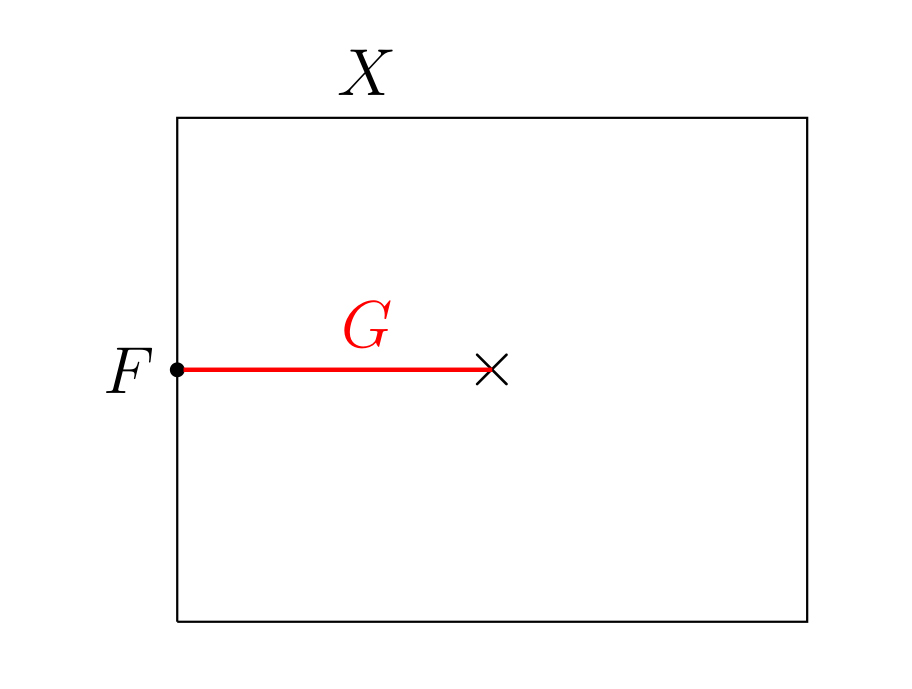
\includegraphics[width=0.40\textwidth]{figures/fig4_1.png}
\caption{相对停点。图内 $X$ 为流形，$F$ 与 $G$ 为相对停点的两个部分。}
\label{fig:rel-stop}
\end{figure}

\begin{thmstar}
设 $X$ 是光滑仿射簇，带嵌入 $X\to\C^N$，该嵌入在 $X$ 上诱导 Stein 结构；设
$f,g\colon X\to\C$ 是 $\C^N$ 上多项式函数的限制。若 $f$ 只有一个临界纤维
$f^{-1}(0)$，则对充分小的 $t\neq0$，存在全忠实函子
\[
\cW(f^{-1}(t),g)\to\cW(X\times\C,z(f-t),g).
\]
\end{thmstar}

\transnote{易错预警：原书在此重述引言中的定理 \ref{thm:relative}（相对版本），并沿用原编号。
译本同样用无编号的 thmstar 环境重述，编号引定理 \ref{thm:relative}，以免自动编号另起
新号、把后文的定义挤位。}

这里第二个范畴关于 $g$ 逐纤维带停点，如 [AA21] 中那样：可容拉格朗日子流形在原映射
$f\colon X\to\C$ 下纤维化于弧之上，同时在 $f$ 的纤维内关于限制 $g|_{f^{-1}(t)}$ 可容。

\begin{definition}\label{def:4-1-1}
给定 Stein 流形 $X$ 与两个全纯函数 $f,g\colon X\to\C$，定义相对 Fukaya--Seidel 范畴
（relative Fukaya--Seidel category）$\cW(X,f,g)$ 为 $X$ 的 wrapped Fukaya 范畴
$\cW(X,F\cup G)$，其相对停点（relative stop）由以下两者的并给出：
\begin{itemize}
\item $F$：扇形 $(f^{-1}(-\infty),g)$ 的相对骨架（relative skeleton），位于
$\partial^\infty X$ 内；
\item $G$：$(g|_{f^{-1}(t)})^{-1}(-\infty)\subseteq\partial^\infty f^{-1}(t)\subseteq
\partial^\infty X$ 的并，其中 $t$ 沿一条连接 $-\infty$ 与 $0$ 的弧取值；
\end{itemize}
如图 \ref{fig:rel-stop} 所示。
\end{definition}

\transnote{易错预警：定义 \ref{def:4-1-1} 中的 $F$、$G$ 是两族边界集，不是函数。相对
停点取 $F\cup G$：$F$ 是扇形 $(f^{-1}(-\infty),g)$ 的相对骨架，$G$ 是沿一条弧变化的一族
停点之并。后文说「附加手柄的余核 $\ell$」时，$\ell$ 与这里的 $F$、$G$ 无关。}

这个停点可以看作相对骨架在无穷远处的边界。

\transnote{含糊点拨：原书这句跨 p.64--65，且页图在 p.64 末行与 p.65 首行重复出现
「relative skeleton」，疑为底本笔误。译文合并为一句，只保留一次「相对骨架」，并在报告
疑点中列明。}

% EN49 c07 | 原书 p.65–75（PDF 76–86） | 第 4 章 §4.2
% 骨架文件：标题行已设定，正文由译者填写。每页起首用 % ===== 原书 p.N ===== 注释标记。
\subsection{主定理的证明}

% ===== 原书 p.65 =====
后文我们将在关于 $f$、$g$ 与 $X$ 的强假设下证明：相对 Fukaya--Seidel 范畴确实等价于
Fukaya--Seidel 范畴 $\cW(X,f+\delta g)$，其中 $\delta>0$ 充分小。一般而言这个等价当然
不应成立。

由于这一构造，定理 \ref{thm:aak-equiv} 的证明可以原样搬来，说明在临界轨迹中的可容
拉格朗日子流形上取顶针，给出全忠实函子
\[
T\colon\cW(f^{-1}(t),g)\to\cW(X\times\C,z(f-t),g).
\]
在适当修改命题 \ref{prop:3-0-5} 之后，我们预期它是一个等价。

由于要考虑两个 Landau--Ginzburg 模型，为相应的 cap 函子与 cup 函子建立记号很重要：

\begin{itemize}
\item 对 Landau--Ginzburg 模型 $(X,f)$，我们用
$\cap\colon D\cW(X,f)\to D\cW(f^{-1}(t))$，\\
与 $\cup\colon D\cW(f^{-1}(t))\to D\cW(X,f)$；
\item 对 Landau--Ginzburg 模型 $(X\times\C,F_t)$，则改用记号
$\bigcap\colon D\cW(X\times\C,F_t)\to D\cW(X\setminus f^{-1}(t))$，\\
与 $\bigcup\colon D\cW(X\setminus f^{-1}(t))\to D\cW(X\times\C,F_t)$。
\end{itemize}

\transnote{易错预警：本节的 cap 与 cup 函子有两套记号。模型 $(X,f)$ 用小的
$\cap$、$\cup$；模型 $(X\times\C,F_t)$ 用大的 $\bigcap$、$\bigcup$。文字层把大符号识别成
拉丁字母 T 与 S，对照页图时务必分清：正文里的 $\bigcup\ell$ 不是「$S\ell$」，
$\bigcap$ 也不是 AAK 等价里的函子 $T$。}

我们将经命题 \ref{prop:3-0-5} 构造的 Viterbo 限制映射（Viterbo restriction map），把
$D\cW(X\setminus f^{-1}(t),f)$ 的对象看作 $D\cW(X,f)$ 的对象。

我们的结果将由下述事实推出：在定理 \ref{thm:aak-equiv} 的 AAK 等价下，作用于附加手柄
的余核 $\ell\subseteq X$ 的 cap 函子

% ===== 原书 p.66 =====
$\cap\colon\cW(X,f)\to\cW(f^{-1}(t))$ 所给出的对象，在 $\cW(X\times\C,z(f-t))$ 中同构于
该附加手柄的核心关于 $X\setminus f^{-1}(t)$ 上 Liouville 结构的环绕圆盘。由
[GPS19, §7.2]，这些手柄的环绕圆盘由 cup 函子
$\bigcup\colon\cW(X\setminus f^{-1}(t))\to\cW(X\times\C,z(f-t))$ 作用于手柄的余核 $\ell$
给出。因此该同构正是 [AS15, Lemma A.28]；可惜其中勾勒的证明难以严格化。该同构也可由
[AG] 中构造的伴随给出的大形式论证推出。这里我们给出一个不依赖 [AG] 的替代论证。

\transnote{背景直觉：这一步要把「环绕圆盘」与「余核在 cap 函子下的像」等同起来，本质上是
把手柄分解一侧的几何翻译成 Fukaya 范畴里的对象。Yoneda 引理随后把对象层面的同构升级为
左模的同构，这才足以锁定 $A_\infty$ 结构。}

对 $A_\infty$ 范畴使用 Yoneda 引理 [Sei08b, Corollary 14.7]，我们要证的便是：

\begin{theorem}\label{thm:4-2-1}
对每个附加余核 $\ell$，存在 $\cW(f^{-1}(t))$ 上左模（left module）的等价
\[
T^*\cY_{\bigcup(\ell)}\cong\cY_{\cap\ell},
\]
其中 $\cY\colon\cW(f^{-1}(t))\to\cW(f^{-1}(t))\mathrm{Mod}$ 是左 Yoneda 函子（left Yoneda functor），
$T^*$ 表示左模的拉回。
\end{theorem}

\transnote{含糊点拨：记号 $\cW(f^{-1}(t))\mathrm{Mod}$ 指该范畴上左模范畴，$\mathrm{Mod}$
用直立体、不加空格。$T^*$ 只在左模层面有定义（不是几何上的拉回），故本定理的比较发生在
模范畴里。}

\begin{proof}
本证明继续使用上面在 $X\times\C$ 上构造的 Liouville 结构。注意关于诱导的 Liouville
结构，$F_t$ 的每个纤维都含一个微分同胚于 $f^{-1}(t)\times\C^*$ 的开邻域，其中的
Liouville 向量场由与标准 Liouville 向量场的乘积给出：
\[
Z=-\frac{\varepsilon}{r^3}\partial_r,
\]
其中 $r=|z|$ 是径向坐标。

% ===== 原书 p.67 =====
给定 $\cW(f^{-1}(t))$ 中任一拉格朗日子流形 $L$，顶针 $TL$ 与 $\bigcup\ell$ 在 $F_t$ 的
同一个纤维中相交，设在 $0<\delta\in\C$ 所对应的纤维上；这里取 $\delta>0$ 充分小，使
$B_\delta$ 上方 $TL$ 完全落在 Morse--Bott 模型内。由于乘积结构，在纤维
$F_t^{-1}(\delta)$ 中 $TL$ 由 $L\times K\subseteq f^{-1}(t)\times\C^*\subseteq
X\setminus f^{-1}(t)$ 给出，其中 $K\subseteq\C^*$ 是绕 $0$ 的小圆周。按 cup 函子的
定义，$\bigcup\ell$ 在该纤维 $F_t^{-1}(\delta)$ 中正好由余核 $\ell$ 给出；见
图 \ref{fig:mod-gvs}。

\transnote{易错预警：原文写「$0<\delta\in\C$」，$\C$ 上并没有序，这里的 $\delta$ 实际是
小的正实数，只是借用 $\C$ 的实轴来定位纤维。译文照录，读者按正实数理解即可。}

注意到在命题 \ref{prop:3-0-3} 对 $X\setminus f^{-1}(t)$ 上 Stein 结构的分析中，每个
附加余核的边界必落在 $f^{-1}(t)$ 中：它们不能留在紧集内，因为 Stein 函数没有指标
$(n+1)$ 的临界点；它们也不能以 $|f-t|^{-1}(\delta)$ 为边界，因为 Liouville 向量场指向
内部。我们在 $X\times\C$ 上用来定义 Fukaya 范畴的 Liouville 结构是该 Stein 结构的形变，
但这个正合形变保持 Liouville 向量场的流线。由于 Liouville 向量场在
$f^{-1}(t)\times\C^*\subseteq X\setminus f^{-1}(t)$ 上的局部形状，这意味着 $\ell$
纤维化于 $\C^*$ 之上，因而与 $L\times K$ 在 $f$ 的同一个纤维中相交。在该纤维内，按 cap
函子的定义，$\bigcup\ell$ 由 $\cap\ell$ 给出；因此 $TL$ 与 $\bigcup\ell$ 正好沿
$L\cap(\cap\ell)\subseteq f^{-1}(t)$ 相交；见图 \ref{fig:mod-gvs}。于是得到向量空间的
同构：
\[
T^*\cY_{\bigcup(\ell)}(L)=CF\left(\bigcup\ell,TL\right)
\cong CF(\cap\ell,L)=\cY_{\cap\ell}(L).
\]
又由马斯洛夫指数在乘积下的可加性，这实际上是分次向量空间的同构。还需匹配
$A_\infty$ 模运算 $\mu^k$。

\transnote{含糊点拨：$|f-t|^{-1}(\delta)$ 指函数 $|f-t|$ 的 $\delta$ 水平集，与纤维
记号 $f^{-1}$ 不是一回事；原文两种上标 $-1$ 混用，中文只能照译并在此提示。}

我们从微分 $\mu^1$ 开始。此时 $TL$ 与 $\bigcup\ell$ 的交集落在纤维 $f^{-1}(t)$ 内，而该
纤维含于 $F_t^{-1}(\delta)$ 中。

% ===== 原书 p.68 =====
\begin{figure}[htbp]
\centering
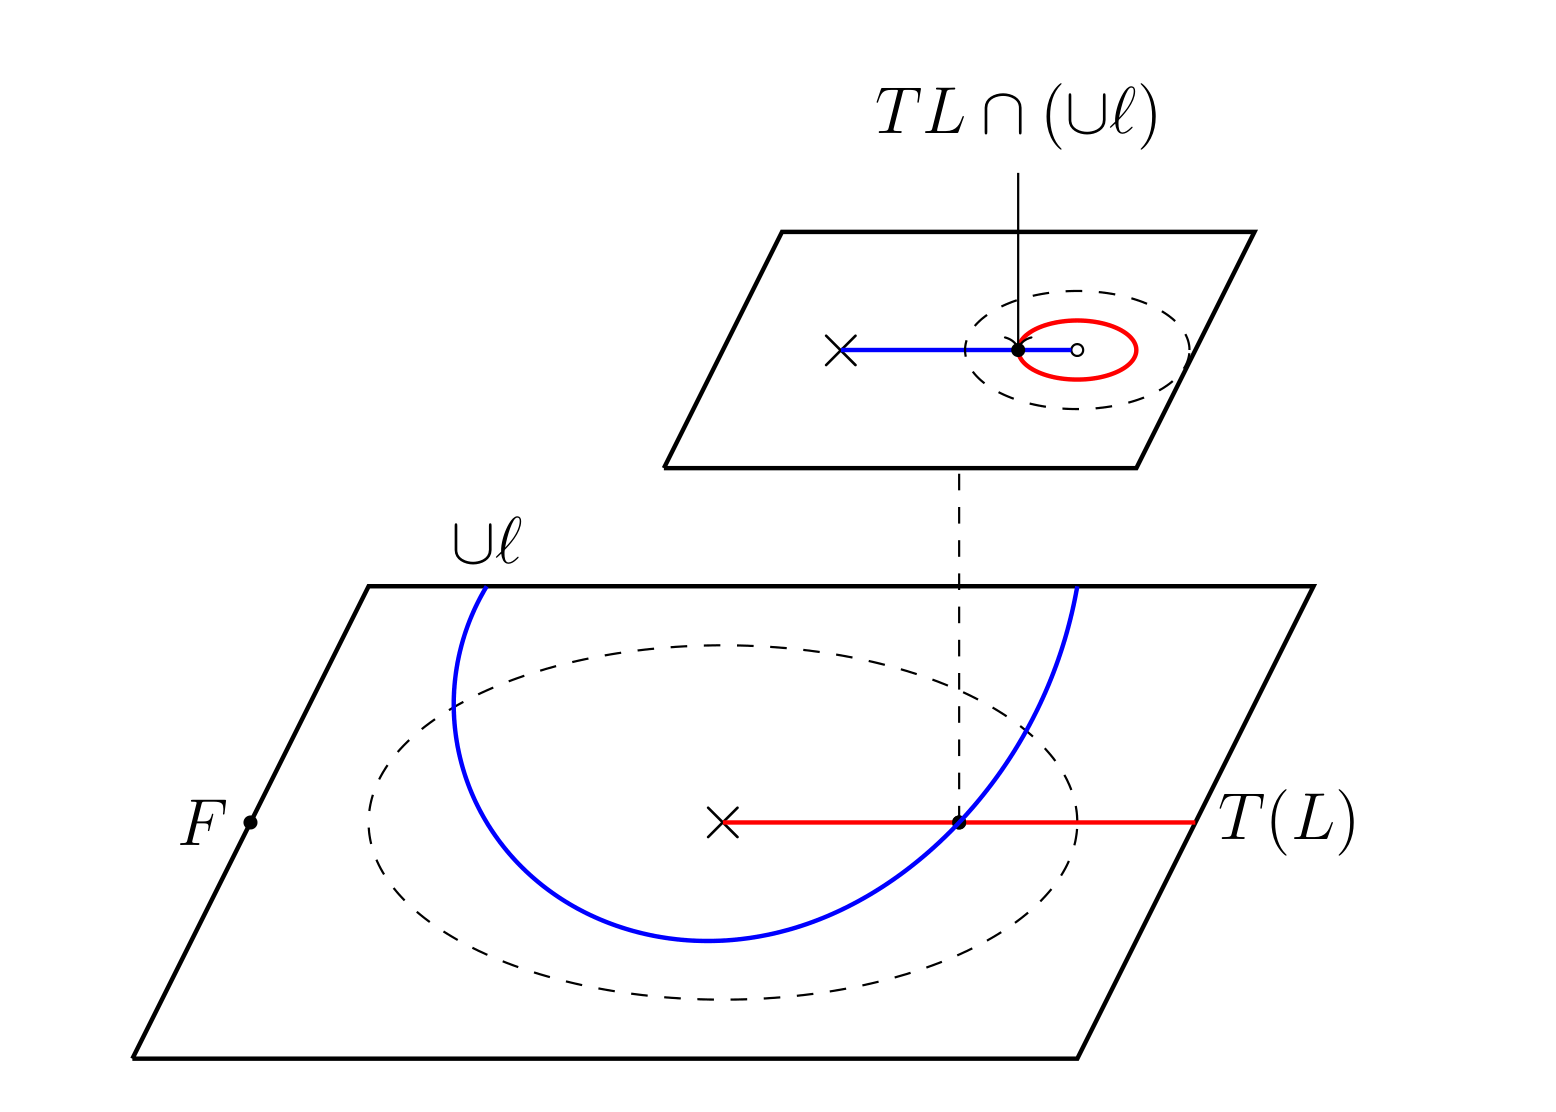
\includegraphics[width=0.72\textwidth]{figures/fig4_2.png}
\caption{把各模识别为分次向量空间。}
\label{fig:mod-gvs}
\end{figure}

把定理 \ref{thm:aak-equiv} 中的极大值原理论证迭代用于全纯映射 $F_t$ 与 $f$，即知计算
$\mu^1\colon T^*\cY_{\bigcup(\ell)}(L)\to T^*\cY_{\bigcup(\ell)}(L)$ 的全纯圆盘全部落在
该纤维 $f^{-1}(t)\subseteq F_t^{-1}(\delta)$ 内；再把那里的横截性论证稍作变化便知，任何
用于使 $f^{-1}(t)$ 内圆盘横截的近复结构，都可延拓到 $X\times\C$，使总空间中计算 $\mu^1$
的圆盘也正则。

\transnote{易错预警：这里用的是定理 \ref{thm:aak-equiv} 证明中「极大值原理把圆盘压进
$F_t^{-1}(0)$、再压进 $f^{-1}(t)$」的迭代版本；两次极大值原理对应两次投影（$F_t$ 与
$f$），不要误当作一次。}

现在把乘积运算 $\mu^2$ 当作后续论证的简化原型。设 $L_1,L_2$ 是 $f^{-1}(t)$ 中的正合
柱状拉格朗日子流形，令 $T^{(i)}L_i=T_i^{(i)}$ 为它们如定理 \ref{thm:aak-equiv} 的证明中
那样的顶针。设有交点 $y_1\in(\cap\ell)\cap L_1$、$x\in L_1\cap L_2$ 与
$y_2\in T^{(2)}L_2\cap(\cap\ell)$，并对定义以下运算的圆盘模空间
$\cM_J^{f^{-1}(t)}(y_1,x,y_2)$，在 $f^{-1}(t)$ 上选取正则的近复结构 $J$（依赖于定义域
与共形结构）：

% ===== 原书 p.69 =====
\[
CF(L_2,L_1)\otimes\cY_{\cap\ell}(L_2)\to\cY_{\cap\ell}(L_1).
\]

把这些近复结构延拓为 $X\times\C$ 上的近复结构，使其在邻域 $f^{-1}(t)\times\C$ 上为
乘积型；延拓后的结构仍记为 $J$。

由定理 \ref{thm:aak-equiv} 与上述论证，这些交点对应于以下交点：
$y_1\in\bigcup\ell\cap T^{(1)}L_1$，落在 $F_t^{-1}(\delta)$ 中；
$x\in T^{(1)}L_1\cap T^{(2)}L_2$，落在 $F_t^{-1}(0)$ 中；以及
$y_2\in T^{(2)}L_2\cap\bigcup\ell$，按顶针 $T_i^{(i)}$ 的构造落在
$F_t^{-1}(e^{i\theta}\delta)$ 中，其中 $0<\theta<\pi$。现在考虑 $X\times\C$ 内与下述
运算相对应的全纯圆盘模空间 $\cM_J^{X\times\C}(y_1,x,y_2)$：
\[
CF(T^{(2)}L_2,T^{(1)}L_1)\otimes\cY_{\bigcup\ell}(T^{(2)}L_2)
\to\cY_{\bigcup\ell}(T^{(1)}L_1).
\]

所有这些交点都落在局部 Morse--Bott 模型 $f^{-1}(t)\times\C^2$ 内。于是对全纯映射
$F_t$ 与 $f$ 的投影施用 $\C$ 上标准近复结构的极大值原理，所有这些圆盘必落在局部
Morse--Bott 邻域 $f^{-1}(t)\times\C^2\subseteq F_t^{-1}(B_\delta)$ 内。在这个
Morse--Bott 模型内，我们有若干全纯投影。首先，投影到 $f^{-1}(t)$ 给出满射
\[
p\colon\cM_J^{X\times\C}(y_1,x,y_2)\to\cM_J^{f^{-1}(t)}(y_1,x,y_2),
\]
这是因为近复结构就是这样定义的。我们断言它实际上是双射，并且
$\cM_J^{X\times\C}(y_1,x,y_2)$ 关于该近复结构正则。

% ===== 原书 p.70 =====
为看出这一点，设 $(u,r)\in\cM_J^{X\times\C}(y_1,x,y_2)$ 是这样的圆盘，
$u\colon D\to X\times\C$，而 $r$ 是三标点圆盘 $D$ 的唯一共形类（conformal class）；那么可以证明，它由到
$f^{-1}(t)$ 的投影决定，如下。

令 $\pi\colon f^{-1}(t)\times\C^2\to\C^2$ 为到第二个因子的（全纯）投影。考虑从三标点
圆盘 $D$ 到 $\C^2$ 的全纯映射 $\pi\circ u$。由于三标点圆盘的共形等价类唯一，这个全纯
圆盘 $(\pi\circ u,r)$ 计算运算
\[
\mu^2\colon CF(T_2,T_1)\times CF(U,T_2)\to CF(U,T_1),
\]
其中 $T_i,U\subseteq\C^2$ 分别是投影 $\pi(T^{(i)}L_i)$、$\pi(\bigcup\ell)$ 所得的
拉格朗日子流形；见图 \ref{fig:mu2}。这些 $T_i$ 是 $\C^2$ 上标准 Lefschetz 纤维丛的
顶针，因而在原点横截相交。拉格朗日子流形 $U$ 是实轴 $\R_+$ 在模型 Lefschetz 纤维丛
一般纤维 $\{z_1z_2=\delta\}\cong\C^*$ 内的平行移动，因而与每个 $T_i$ 各横截相交于一点。

\transnote{背景直觉：在 $\C^2$ 的模型里，$T_i$ 是 Lefschetz 顶针、$U$ 是实轴的平行
移动，后者与每个顶针恰好横截交于一点。正因为交点如此之少，$\C^2$ 里的模空间只有单个
正则圆盘，$\pi$ 才可能是双射。}

对 $\C^2$ 上一般的近复结构 $J$，该模空间由单个正则圆盘组成，它计算唯一交点
$p\in U\cap T_1$ 与 $T_1\cong T_2$ 的恒等元的乘积。把前面关于 $X\times\C$ 上近复结构的
构造用于此处的 $J$（代替 $\C^2$ 上标准近复结构），便知可以保证：对任何
$(u,r)\in\cM_J^{X\times\C}(y_1,x,y_2)$，$p(u,r)$ 与 $\pi(u,r)$ 都正则。这恰好说明，在
$p$ 下任何 $\cM_J^{f^{-1}(t)}(y_1,x,y_2)$ 中圆盘的原像里只有一个全纯圆盘。容易验证这些
模空间上诱导的定向一致。

对更高的 $\mu^k$ 运算，我们先推广上述关于 $\mu^2$ 的论证。设 $L_i$（$i=1,\dots,k$）
是 $f^{-1}(t)$ 中的正合柱状拉格朗日子流形，并令 $T^{(i)}L_i=T_i^{(i)}$ 为它们如
定理 \ref{thm:aak-equiv} 证明中那样的顶针。

% ===== 原书 p.71 =====
\begin{figure}[htbp]
\centering
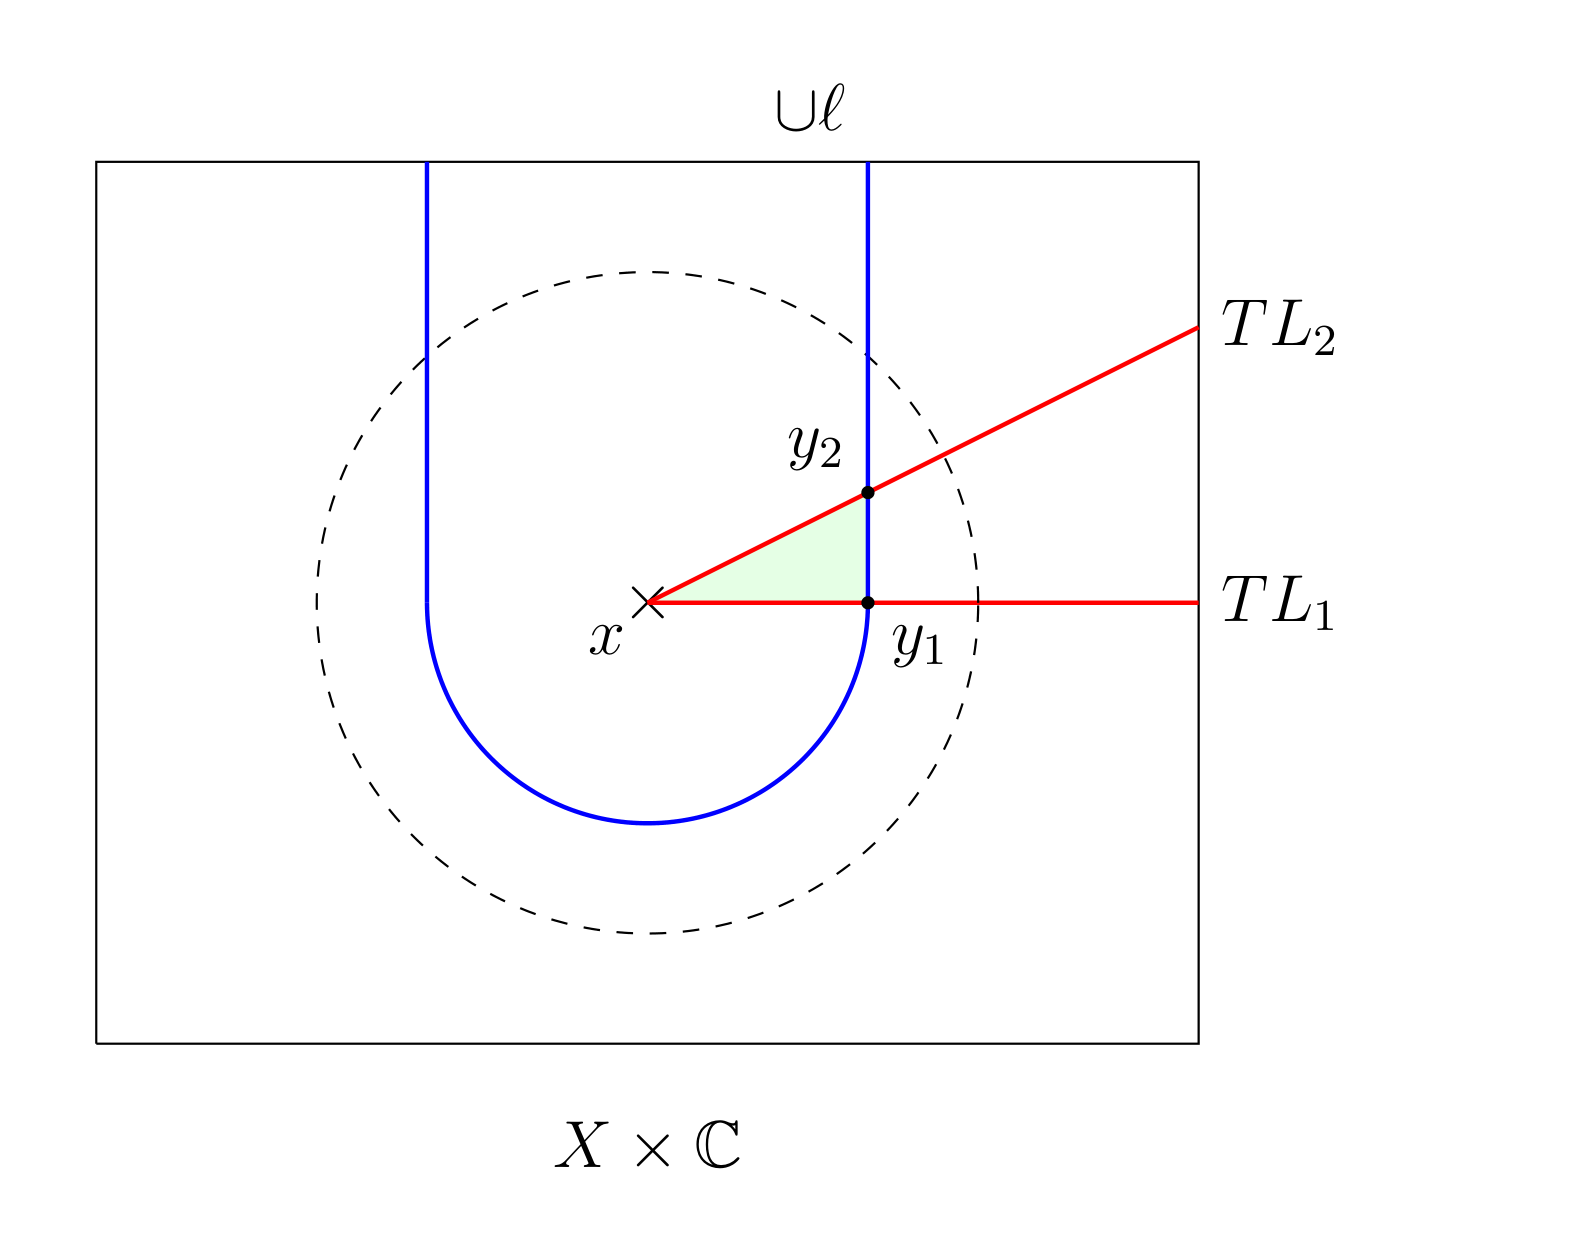
\includegraphics[width=0.72\textwidth]{figures/fig4_3.png}
\caption{把模上的 $\mu^2$ 运算识别出来：绿色部分是那个全纯圆盘。}
\label{fig:mu2}
\end{figure}

设有交点 $y_1\in(\cap\ell)\cap L_1$、$x_i\in L_i\cap L_{i+1}$（$i=1,\dots,k-1$）与
$y_2\in T^{(k)}L_k\cap(\cap\ell)$，并对定义以下运算的圆盘模空间
$\cM_J^{k,f^{-1}(t)}(y_1,x_1,\dots,x_k,y_2)$，在 $f^{-1}(t)$ 上选取正则的近复结构
$J$（依赖于定义域与共形结构）：
\[
CF(L_2,L_1)\otimes\cdots\otimes CF(L_k,L_{k-1})\otimes\cY_{\cap\ell}(L_k)
\to\cY_{\cap\ell}(L_1).
\]
把这些近复结构延拓为 $X\times\C$ 上的近复结构，使其在邻域 $f^{-1}(t)\times\C$ 上为
乘积型。

% ===== 原书 p.72 =====
由定理 \ref{thm:aak-equiv} 与上述论证，这些交点对应于以下交点：
$y_1\in\bigcup\ell\cap T^{(1)}L_1$，落在 $F_t^{-1}(\delta)$ 中；
$x_i\in T^{(i)}L_i\cap T^{(i+1)}L_{i+1}$（$i=1,\dots,k-1$），落在 $F_t^{-1}(0)$ 中；
以及 $y_2\in T^{(k)}L_k\cap\bigcup\ell$，按顶针 $T_i^{(i)}$ 的构造落在
$F_t^{-1}(e^{i\theta}\delta)$ 中，其中 $0<\theta<\pi$。现在考虑 $X\times\C$ 内与下述
运算相对应的全纯圆盘模空间
$\cM_J^{k,X\times\C}(y_1,x_1,\dots,x_k,y_2)$：
\[
\begin{gathered}
CF(T^{(2)}L_2,T^{(1)}L_1)\otimes\cdots\otimes
CF(T^{(k)}L_k,T^{(k-1)}L_{k-1})\\
\otimes\cY_{\bigcup\ell}(T^{(k)}L_k)\to\cY_{\bigcup\ell}(T^{(1)}L_1).
\end{gathered}
\]

所有这些交点都落在局部 Morse--Bott 模型 $f^{-1}(t)\times\C^2$ 内。于是对全纯映射
$F_t$ 与 $f$ 的投影施用 $\C$ 上标准近复结构的极大值原理，所有这些圆盘必落在局部
Morse--Bott 邻域 $f^{-1}(t)\times\C^2\subseteq F_t^{-1}(B_\delta)$ 内。在这个
Morse--Bott 模型内，我们有若干全纯投影。首先，投影到 $f^{-1}(t)$ 给出满射
\[
p\colon\cM_J^{k,X\times\C}(y_1,x_1,\dots,x_k,y_2)\to
\cM_J^{k,f^{-1}(t)}(y_1,x_1,\dots,x_k,y_2),
\]
这是因为近复结构就是这样定义的。我们断言它实际上是双射，且
$\cM_J^{k,X\times\C}(y_1,x_1,\dots,x_k,y_2)$ 关于该近复结构正则（如前，可以验证这些
模空间上诱导的定向一致）。为说明这一点，设
$(u,r)\in\cM_J^{k,X\times\C}(y_1,x_1,\dots,x_k,y_2)$ 是这样的圆盘，
$u\colon D\to X\times\C$，而 $r$ 是标点圆盘（marked disk）的固定共形类；那么可以证明，它由到
$f^{-1}(t)$ 的投影决定，如下。

令 $\pi\colon f^{-1}(t)\times\C^2\to\C^2$ 为到第二个因子的（全纯）投影。考虑全纯映射
$\pi\circ u$，我们同样想说明：在 $p$ 下任何
$\cM_J^{k,f^{-1}(t)}(y_1,x_1,\dots,x_k,y_2)$ 中圆盘的原像里只有一个全纯圆盘。由于共形
类 $r$ 已固定，圆盘 $\pi\circ u$ 不再计算 $A_\infty$ 运算 $\mu^k$。这个全纯圆盘
$(\pi\circ u,r)$ 的边界仍落在如上所得的投影 $\pi(T^{(i)}L_i)$、$\pi(\bigcup\ell)$
给出的拉格朗日子流形 $T_i,U\subseteq\C^2$ 上，并在交点处成角：

% ===== 原书 p.73 =====
\begin{figure}[htbp]
\centering
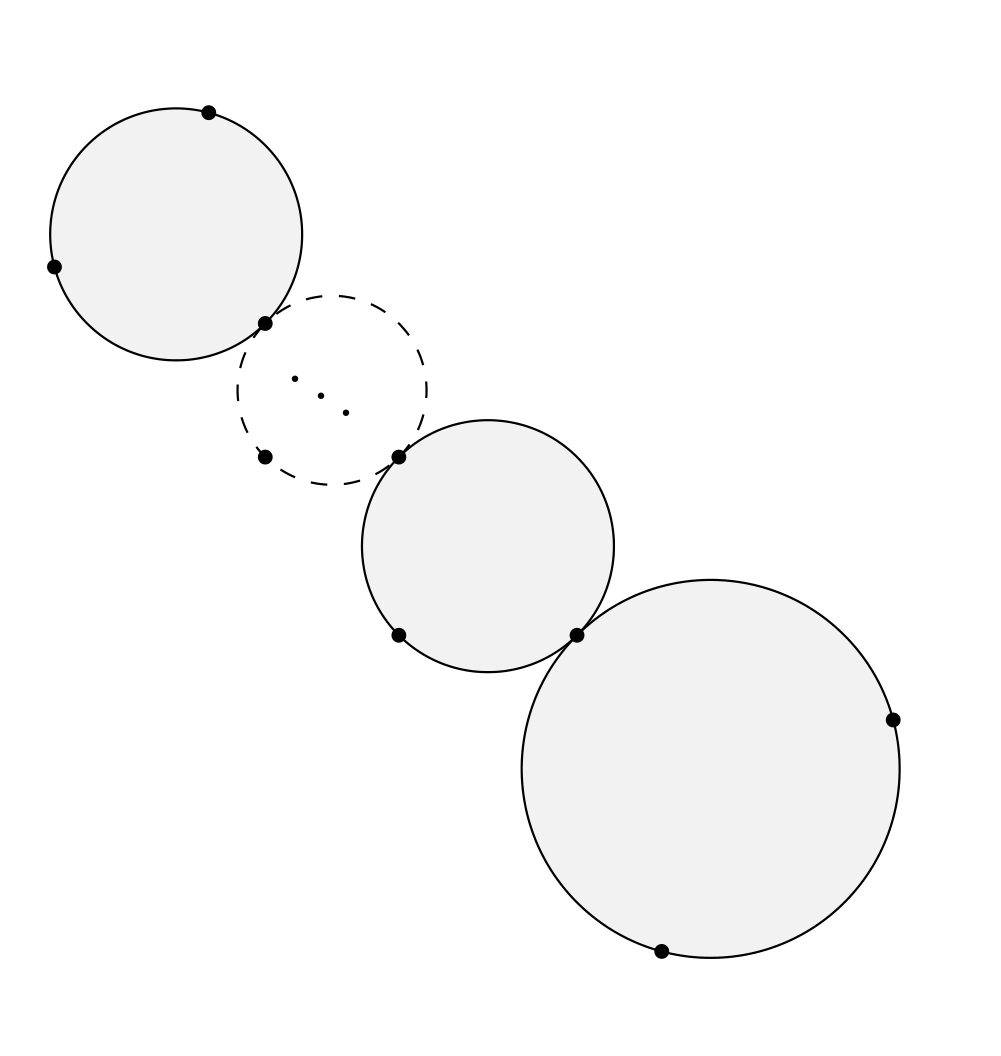
\includegraphics[width=0.44\textwidth]{figures/fig4_4.png}
\caption{三个三标点全纯圆盘构成的单腿树。}
\label{fig:tree}
\end{figure}

$p_1\in U\cap T_1$、$p_k\in U\cap T_k$，以及 $T_i\cong T_{i+1}$ 的恒等元
$a_i\in T_i\cap T_{i+1}$。

\transnote{含糊点拨：底本这一句在 p.72 末只写到「与交点处成角」，p.73 首因插图隔开，
才接上 $p_1\in U\cap T_1,\dots$。译文把「成角：」留在前段、把角点列表接在插图上端，
读起来语义不断。}

现在选取 $\gamma\colon[0,1)\to\overline{\cS}_k$，它是 $(k+1)$ 标点圆盘紧化模空间中
一条光滑简单道路（即一族共形结构），从固定的共形结构 $r=\gamma(0)$ 出发，走向最深的
边界层 $r_0=\lim_{t\to1^-}\gamma(t)$，在那里 $r$ 退化为单腿三叉圆盘树 $r_0$，即单腿树（one-legged tree），
见图 \ref{fig:tree}。现在考虑参数化模空间（parametrized moduli space）
$\widetilde{\cM}_J^{k,\C^2}(p_1,a_1,\dots,a_{k-1},p_k)$：其中的 $(v,s)$ 是 $\C^2$ 中
$J$-全纯圆盘，边界条件与 $u$ 相同，但定义域上的共形结构 $s$ 允许沿道路 $\gamma$ 变动。
标准论证表明，对 $\C^2$ 上一般的近复结构 $J$，该模空间成为光滑的一维流形。再次把前面
关于 $X\times\C$ 上近复结构的构造用于修改后的 $J$（代替 $\C^2$ 上标准近复结构），便知
可以保证：对任何 $(u,r)\in\cM_J^{k,X\times\C}(y_1,x_1,\dots,x_k,y_2)$，$p(u,r)$ 与
$\pi(u,r)$ 也都正则。

\transnote{易错预警：带波浪号的 $\widetilde{\cM}$ 是参数化模空间，其定义域的共形结构
沿道路 $\gamma$ 变动，不要与普通模空间 $\cM$ 混同；$r$ 是共形类，不是半径。}

现在考虑 $\widetilde{\cM}_J^{k,\C^2}(p_1,a_1,\dots,a_{k-1},p_k)$ 的 Gromov 紧化（Gromov compactification）。
对纤维丛 $\C^2\to\C$ 施用极大值原理，该模空间中的圆盘不可能逃逸到无穷远，

% ===== 原书 p.74 =====
因而可施用 Gromov 紧性。正合性排除圆盘泡与球泡（bubbling）；又因 $p_1$、$a_i$、$p_k$ 次数相同，
不会发生条带破裂（strip breaking）。于是
$\widetilde{\cM}_J^{k,\C^2}(p_1,a_1,\dots,a_{k-1},p_k)$ 的边界分支只来自道路 $\gamma$
两端的定义域共形结构。在 $0$ 端，共形结构是 $\gamma(0)=r$，故 Gromov 边界的一部分由
固定共形结构 $r$ 的圆盘模空间给出。在另一端，$\lim_{t\to1^-}\gamma(t)=r_0$；该边界
分支由贡献于迭代乘积运算
\[
\mu^2(\mu^2(\cdots\mu^2(a_1,a_2)\cdots),a_{k-1}),p_k)=p_1
\]
的圆盘组成，其中 $p_k\in U\cap T_k$，$a_i$ 是 $T_i\cong T_{i+1}$ 的恒等元。如上所述，
每个这样的乘积运算在 $\C^2$ 中都有唯一的全纯圆盘表示，因而这样的圆盘只有一个。于是，
由于 $\widetilde{\cM}_J^{k,\C^2}(p_1,a_1,\dots,a_{k-1},p_k)$ 是带边界的一维流形，
在投影 $\pi$ 到 $\C^2$ 下必恰有一个共形类为 $r$ 的圆盘 $(u,r)$。
\end{proof}

现在可以证明主要结果。

\begin{thmstar}
设 $X$ 是光滑仿射簇，带嵌入 $X\to\C^N$，该嵌入在 $X$ 上诱导 Stein 结构；设
$f\colon X\to\C$ 是 $\C^N$ 上多项式函数的限制。若 $f$ 只有一个临界纤维
$f^{-1}(0)$，则对充分小的 $t\neq0$，存在 $A_\infty$ 范畴的拟等价
\[
D^\pi\cW(f^{-1}(t))[s^{-1}]\to D^\pi\cW(X\times\C,zf).
\]
\end{thmstar}

\transnote{易错预警：原书在证明主定理前重述引言中的定理 \ref{thm:knorrer}（导出 Knörrer 周期性），
并沿用编号「1.3.1」。译本同样用无编号的 thmstar 环境，编号引
定理 \ref{thm:knorrer}，以免自动编号另起新号。}

% ===== 原书 p.75 =====
\begin{proof}
这由前面的结果合并得到。把论证明确写出来：
\begin{itemize}
\item 由推论 \ref{cor:2-3-2}，$\cW(f^{-1}(0))$ 是 $\cW(f^{-1}(t))$ 对由形如
$\cap L$ 的拉格朗日子流形生成的子范畴 $\cD'$ 的商；
\item 由命题 \ref{prop:3-0-5}，该子范畴 $\cD'$ 与由 $\cap\ell$（$\ell$ 取遍附加余核）
生成的子范畴相同；
\item 由定理 \ref{thm:aak-equiv}，$\cW(f^{-1}(t))$ 等价于
$\cW(X\times\C,z(f-t))$；在该等价下，$\cD'$ 的生成元 $\cap\ell$ 由
定理 \ref{thm:4-2-1} 送到子范畴 $\cD$ 的对象 $\bigcup\ell$；
\item 由命题 \ref{prop:3-0-4}，$\cW(X\times\C,z(f-t))$ 对子范畴 $\cD$ 的商给出
$\cW(X\times\C,zf)$。
\end{itemize}
于是
\[
D^\pi\cW(f^{-1}(0))\cong D^\pi\cW(f^{-1}(t))/\cD'
\cong D^\pi\cW(X\times\C,z(f-t))/\cD\cong D^\pi\cW(X\times\C,zf).
\]
\end{proof}

\transnote{含糊点拨：$\cD'$ 与 $\cD$ 是两个不同的子范畴：$\cD'$ 由 $f^{-1}(t)$ 一侧的
$\cap L$ 生成，$\cD$ 由 $X\times\C$ 一侧的 $\bigcup\ell$ 生成，定理 \ref{thm:4-2-1}
正是说二者在 AAK 等价下彼此对应。链式同构的三步依次用推论 \ref{cor:2-3-2}、
定理 \ref{thm:aak-equiv} 与命题 \ref{prop:3-0-4}。}

\clearpage
% EN49 c08 | 原书 原书 p.76–86（PDF 87–97） | 第 5 章 §5.1–5.3
% 骨架文件：标题行已设定，正文由译者填写。每页起首用 % ===== 原书 p.N ===== 注释标记。
\section{镜像对称的应用}

% ===== 原书 p.76 =====
在下文关于镜像对称的应用中，我们将用到代数几何中的下述引理。证明相当简单，其梗概可见
[Sei08a, p.5]。设 $X$ 是光滑拟射影代数簇，$L$ 是带截面 $s$ 的线丛，并令
$U=X\setminus s^{-1}(0)$。

\begin{lemma}\label{lem:5-0-1}
设 $s\colon L^{-1}\otimes-\to\id$ 是由乘以截面 $s$ 给出的自然变换。则在 $s$ 处局部化
给出范畴等价
\[
\operatorname{Coh}(X)[s^{-1}]\simeq\operatorname{Coh}(U).
\]
\end{lemma}

\transnote{易错预警：原书此式印作 $s\colon L^{-1}\otimes\to\id$，$\otimes$ 后漏排了作用对
象；按上下文应读作自然变换 $L^{-1}\otimes-\to\id$，即对每个 $F$ 给出
$L^{-1}\otimes F\to F$。译文补上占位符「$-$」；原书在 p.80、p.85 还有两处同样的漏排，
译文一律照此处理，不再逐处注明。}

对这一引理的一种启发式解读是：局部化把镜像对称一侧「去掉一个除子」与另一侧「退化到特殊
纤维」联系了起来。

\transnote{背景直觉：引理 \ref{lem:5-0-1} 是全章的技术枢纽。B 侧去掉除子
$s^{-1}(0)$，等价于把相干层范畴在该截面给出的自然变换处局部化；A 侧沿同一自然变换局部
化，则得到奇异纤维的 Fukaya 范畴。两侧的局部化一旦对上，镜像对称就化归为光滑情形的已
知结论。}

% ===== 原书 p.77 =====
\subsection{裤子塔（tower of pants）}

Landau--Ginzburg 模型 $(\C^{n+1},W_n=z_1\cdots z_{n+1})$ 在镜像对称中具有特殊的重要
性：它是高维裤子 $\Pi_{n-1}=\{x_1+\cdots+x_n+1=0\}\subseteq(\C^*)^n$ 的镜像，例如见
[Nad19a; AAK16]。本节将借助 Abouzaid--Auroux 的工作 [AA21]，在这一特殊情形下勾勒镜像对
称与周期性的另一个证明。

\transnote{易错预警：裤子的下标等于变量个数减一。原书在本段写 $\Pi_{n-1}\subseteq
(\C^*)^n$（$n$ 个变量），到 p.78 又写 $\Pi_n\subseteq(\C^*)^{n+1}$（$n+1$ 个变量），两
处并不矛盾；第 1 章已把 $\Pi_n$ 定义为
$\{x_1+\cdots+x_{n+1}+1=0\}\subseteq(\C^*)^{n+1}$，与本段一致。}

对该 LG 模型，一般纤维 $W_n^{-1}(1)$ 由复环面 $(\C^*)^n$ 给出。我们知道它的 wrapped
Fukaya 范畴由单个拉格朗日量 $L=(\R_+)^n\subseteq(\C^*)^n$ 生成，自同态代数由
$\C[x_1^{\pm1},\dots,x_n^{\pm1}]$ 给出。我们将用到 Abouzaid--Auroux 宣布的下述结果：

\begin{thmstar}
（Abouzaid--Auroux [AA21]）\quad 范畴 $\cW(\C^{n+1},z_1\cdots z_{n+1})$ 由单个拉格朗
日量 $\cup L$ 生成。此外，该 LG 模型一般纤维上的 Seidel 自然变换 $s$ 对应态射
$L\to L$，由乘以 $x_1+\cdots+x_n+1$ 给出。
\end{thmstar}

\transnote{含糊点拨：原文说这两个结果由 Abouzaid--Auroux「announced」（宣布），即作者写作时
尚未正式成文，译本照译作「宣布」。$\cup$ 形符号另记由若干拉格朗日量经 cup 函子粘成的对
象，不是集合的并。例如 $\cup L$ 表示把 $L$ 沿 $\cup$ 函子的一份拷贝粘上去。}

自然变换中求和式 $x_1+\cdots+x_n+1$ 的每一项，对应经过该 LG 模型奇异纤维
$z_1\cdots z_{n+1}=0$ 中某个超平面 $z_i=0$ 的全纯曲线计数。

\begin{corollary}\label{cor:5-1-1}
存在范畴拟等价
\[
D^\pi\cW(W_n^{-1}(0))\simeq D^\pi\cW(\C^{n+2},z_1\cdots z_{n+2})\simeq
\operatorname{Coh}(\Pi_n).
\]
\end{corollary}

% ===== 原书 p.78 =====
\begin{figure}[htbp]
\centering
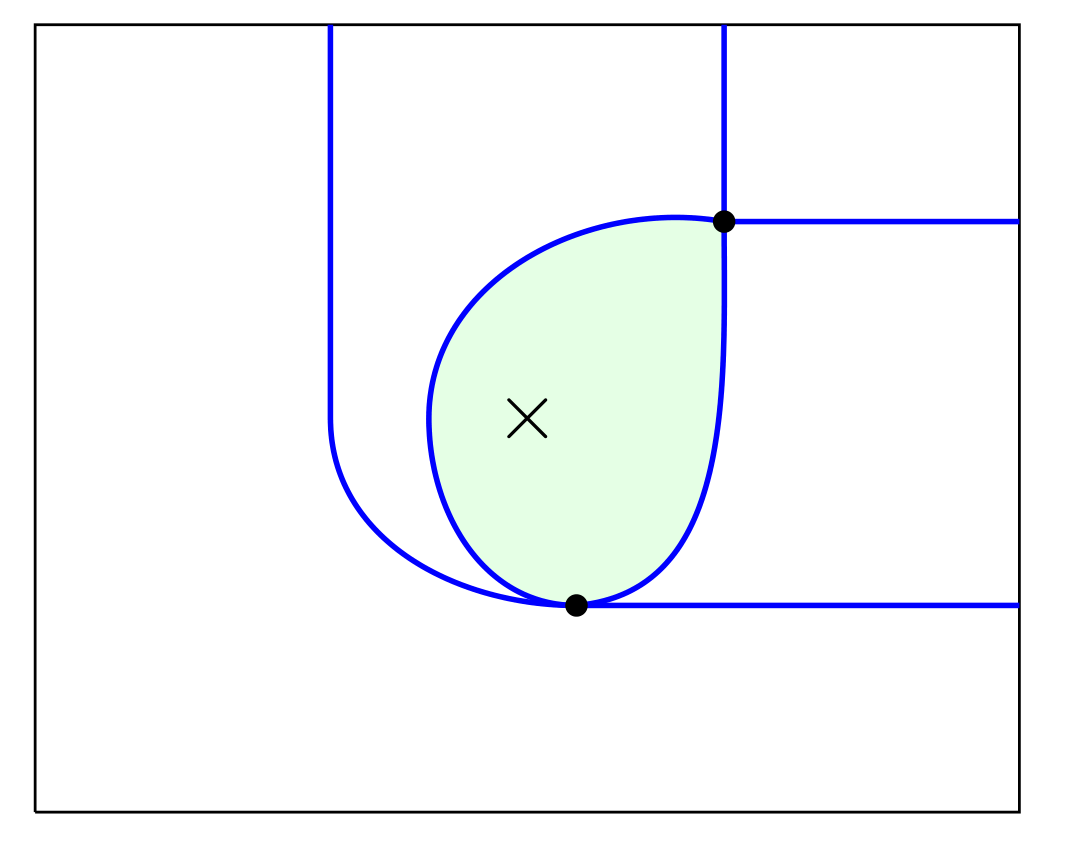
\includegraphics[width=0.38\textwidth]{figures/fig5_1.png}
\caption{计算一个 $\cup$ 形对象的自同态。}
\label{fig:5-1}
\end{figure}

\transnote{背景直觉：图 \ref{fig:5-1} 中的蓝色折线就是原文所称的 $\cup$ 形对象；绿色卵形区域
与两个黑点是辅助标记，图内没有公式或文字标注。证明里说把 $\cup L$ 推离自身，两个黑点正
是推离前后两份拷贝的交点，而自同态代数由该处的映射锥给出。}

\begin{proof}
利用局部化的定义，第一个范畴由 $\C[x_1^{\pm1},\dots,x_n^{\pm1}]$-模范畴在自然变换
$\id\to\id$ 处局部化给出，该自然变换由乘以 $x_1+\cdots+x_n+1$ 给出。这与下述范畴相
同：$\C$-代数 $\C[x_1^{\pm1},\dots,x_n^{\pm1}]$ 在 $x_1+\cdots+x_n+1$ 处局部化上的模
范畴，亦即 $\{x_1+\cdots+x_n+1\neq0\}\subseteq(\C^*)^n$ 上相干层的范畴；但后者恰是
$\{x_1+\cdots+x_n+1=-x_{n+1}\}\subseteq(\C^*)^{n+1}$，即裤子 $\Pi_n$。

第二个范畴可以通过计算生成元 $\cup L$ 的自同态得到。由于 $\cup L$ 由施加 $\cup$ 函子得
到，我们可以把它推离自身，从而看出其自同态代数由映射 $\End(L)\to\End(L)$ 的锥给出，而
该映射由乘以自然变换 $x_1+\cdots+x_{n+1}+1$ 给出（见图 \ref{fig:5-1}）。于是
$\cW(\C^{n+2},z_1\cdots z_{n+2})$ 由 $\C[x_1^{\pm1},\dots,x_{n+1}^{\pm1}]$ 对理想
$(x_1+\cdots+x_{n+1}+1)$ 取商后的模范畴给出。但后者恰是
$\{x_1+\cdots+x_{n+1}+1=0\}\subseteq(\C^*)^{n+1}$ 上相干层的范畴，即裤子 $\Pi_n$。
\end{proof}

应当可以把这一证明推广到环簇中超曲面的补集，按照 Abouzaid--Auroux 的想法，做法如下。设
$H\subseteq V$ 是环簇 $V$ 中的超曲面，由截面 $s\in\Gamma(V,\cO(H))$ 定义。

% ===== 原书 p.79 =====
$H\subseteq(\C^*)^n$ 的镜像由一个环簇 LG 模型 $(Y,W_Y)$ 给出 [Aur18]；把
$H\subseteq(\C^*)^n$ 紧化为 $H\subseteq V$ 会给超势增添额外的项，于是镜像是
$(Y,W_Y+\delta W)$：这里 $W$ 视为用于逐纤维缠绕的辅助超势，如 §4 所述。

\transnote{含糊点拨：secondary superpotential 译作「辅助超势」。它不改变 $Y$ 上原有的超
势 $W_Y$，只用来实现逐纤维的缠绕；$\delta W$ 是紧化时新增的项，其下标不加 $Y$，因为它是
$W$ 的修正而非 $W_Y$ 的修正。}

\begin{thmstar}
（Abouzaid--Auroux [AA21]）\quad 一般纤维的 Fukaya--Seidel 范畴
$D^\pi\cW(W_Y^{-1}(t),W)$ 拟等价于 $\operatorname{Coh}(V)$。此外，单值性 $\mu$ 在
$(W_Y^{-1}(t),W)$ 上的作用镜像于与线丛 $\cO(-H)$ 作张量，而自然变换 $\mu\to\id$ 镜像于
定义截面 $s\colon\cO(-H)\to\cO_V$。
\end{thmstar}

因此，我们的定义的一个 LG 版本使我们能断定：$D^\pi\cW(W_Y^{-1}(0),W)$ 等价于
$\operatorname{Coh}(V\setminus H)$，这里用到引理 \ref{lem:5-0-1}。此外，利用定义
\ref{def:sing-ci}，应当可以把这一点推广到 [AA21] 续篇所考虑的环簇中完全交的情形。

\transnote{易错预警：这里截面 $s$ 的方向是 $\cO(-H)\to\cO_V$，与引理 \ref{lem:5-0-1}
中 $L^{-1}\to\cO$ 的方向一致（$L=\cO(H)$）；若把 $s$ 看成 $\cO_V\to\cO(H)$，则论及的
是同一个截面的另一写法，局部化结论不变。}

\subsection{对曲线的应用}

定义 \ref{def:sing-fuk} 在实际计算中往往相当直接，下面的简单例子即可说明。

\begin{example}\label{exam:5-2-1}
考虑标准 Lefschetz 纤维丛 $X=\C^2$ 与 $f=xy$；我们直接计算结点二次曲线
$\{xy=0\}$ 的 Fukaya 范畴 $\cW(\{xy=0\})$。由引理 \ref{lem:2-3-1}，为求
$\cW(\{xy=0\})$，只需用 $\cap$ 的像对 $\cW(\{xy=t\})$ 取商。但在本例中，唯一能对之施
加 $\cap$ 的对象是 $(\C^2,xy)$ 的标准顶针，而 $\cap$ 恰好给出 vanishing cycle
$V\subseteq\{xy=t\}$。于是 $\cW(\{xy=0\})=\cW(\{xy=t\})/\langle V\rangle$。在
$D^\pi\cW(\{xy=t\})$ 与 $\operatorname{Coh}(\C^*)$ 的镜像对称下，$V$ 对应于点
$p\neq0$ 的点层，而商 $\operatorname{Coh}(\C^*)/\langle\cO_p\rangle$ 恰好给出
$\operatorname{Coh}(\C^*\setminus\{p\})$，它拟等价于裤子上的相干层
$\operatorname{Coh}(\Pi_1)$，这与前面的预期一致。
\end{example}

\transnote{易错预警：原书本例末尾印了一个证明结束符（$\square$），但正文中并没有 proof 环
境。译本把整段放在 example 环境内，不另立证明环境，也不补结束符；该处列入报告疑点。}

% ===== 原书 p.80 =====
在本例中，我们还可以利用 [LO06] 中 $A_\infty$ 范畴局部化的显式公式，计算
$\cW(\{xy=0\})$ 的完整 $A_\infty$ 结构。我们将在后续工作中对此多作讨论。

现在考虑亏格 $1$ 的带奇点曲线。考虑由椭圆曲线的 Tate 族给出的映射 $f\colon X\to\C$，
其中 $f^{-1}(0)$ 是带单个结点的椭圆曲线。由 [PZ01; LP12] 等的工作可知，一般纤维的
Fukaya 范畴 $\cF(f^{-1}(t))$ 与镜像椭圆曲线 $E$ 上的相干层范畴
$\operatorname{Coh}(E)$ 导出等价。此时绕该奇点的单值性由绕相应 vanishing cycle 的负
Dehn twist 扭转给出，它把镜像于 $\cO_E$ 的拉格朗日量 $L\subseteq f^{-1}(t)$，送到斜率
$(-1)$ 的拉格朗日量 $\mu(L)\subseteq f^{-1}(t)$，后者镜像于 $E$ 上次数 $(-1)$ 的线丛
$\cL^{-1}$ [PZ01]。由于单值函子由逐纤维平移到 $\mu(L)$ 给出，在这一镜像等价下，$\mu$
镜像于与线丛 $\cL^{-1}$ 作张量（讨论见下文 §5.3）。于是自然变换 $\mu\to\id$ 镜像于态
射 $\cL^{-1}\to\cO_E$，即对偶线丛 $\cL$ 的一个截面 $s$。因此，我们可以把
$\cW(f^{-1}(t))$ 在该自然变换处的局部化，与 $\operatorname{Coh}(E)$ 的局部化作比较。
一方面，由定义 \ref{def:sing-fuk}，$\cF(f^{-1}(t))$ 的这一局部化给出
$\cF(f^{-1}(0))$，即结点曲线的 Fukaya 范畴。在镜像一侧，由引理 \ref{lem:5-0-1}，
$\operatorname{Coh}(E)$ 在由乘以截面 $s$ 给出的自然变换 $\cL^{-1}\otimes-\to\id$ 处
的局部化，恰好给出补集的相干层导出范畴 $\operatorname{Coh}(E\setminus s^{-1}(0))$。

\transnote{含糊点拨：这里的单值函子「逐纤维平移到 $\mu(L)$」指在每个光滑纤维
$f^{-1}(t)$ 内把拉格朗日量平移，使平移量与 $\mu(L)$ 的截面一致；就范畴层面看，这只
改变了对象的位置，不改变其相交图。}

% ===== 原书 p.81 =====
于是我们得到结点椭圆曲线的 wrapped Fukaya 范畴，与单穿孔椭圆曲线的相干层导出范畴之间
的镜像等价。这一论证可以推广，以说明结点更多的椭圆曲线的 Fukaya 范畴，与穿孔数相应
的椭圆曲线导出等价：只需考虑 Gross--Siebert [GS03] 所论的椭圆曲线 $n$-结点退化的单值
性。

这一点还可以通过考虑带结点与穿孔的椭圆曲线加以推广：取 $f\colon X\to\C$ 为 $n$ 穿孔
椭圆曲线的仿射 Tate 族，其中 $f^{-1}(0)$ 是带单个结点与 $n$ 个穿孔的椭圆曲线。利用
[LP12; LP17] 对一般纤维的镜像等价，可以得到下述两族范畴之间的镜像导出等价。一侧是带
$n$ 个穿孔与 $m$ 个结点的椭圆曲线的 wrapped Fukaya 范畴，另一侧是带 $m$ 个穿孔与 $n$
个结点的椭圆曲线的相干层导出范畴（此处用到引理 \ref{lem:5-0-1} 的一个更强版本）。在本例中，由于 $f$
满足定理 \ref{thm:knorrer} 的假设，还有一个镜像等价：带 $m$ 个穿孔与 $n$ 个结点的椭圆
曲线的相干层，与 LG 镜像 $(X\times\C,zf)$ 的 Fukaya--Seidel 范畴等价。

\transnote{含糊点拨：「引理 \ref{lem:5-0-1} 的一个更强版本」指允许一次去掉多个除子的
情形，即对若干截面各自的自然变换同时局部化。原书未写出该版本，译本不补陈述。}

\subsection{推广}

上述椭圆曲线的例子，是更一般的大复结构极限与复环面同调镜像对称之间关系的一些特例。我
们先回顾 Gross--Siebert 在阿贝尔簇的环簇退化背景下的框架（见 [GS16, §2]）。

设 $M$ 是秩 $n$ 的格，$N=\Hom_\Z(M,\Z)$ 是对偶格，$\Gamma\subseteq M$ 是秩 $n$ 的子
格。商 $B=M_\R/\Gamma$ 自然带有整仿射流形的结构。

% ===== 原书 p.82 =====
设 $\cP$ 是 $M_\R$ 的 $\Gamma$-周期多面体分解，$\varphi\colon M_\R\to\R$ 是严格凸的
分段线性函数，其斜率为整数，且对任意 $\gamma\in\Gamma$ 有
\[
\varphi(m+\gamma)=\varphi(m)+\alpha_\gamma(m),
\]
其中 $\alpha_\gamma\colon M_\R\to\R$ 是某个整仿射函数。令 $\check\Gamma$ 为 $N_\R$ 中
的格 $\{\de\alpha_\gamma(m):\gamma\in\Gamma\}$；则商 $\check B=N_\R/\check\Gamma$ 也
带有整仿射流形的结构。离散 Legendre 变换（如 [GS06] 所述）给出 $N_\R$ 的对偶
$\check\Gamma$-周期多面体分解 $\check\cP$，以及严格凸的分段线性函数
$\check\varphi\colon N_\R\to\R$。令 $X(B)$ 为切丛对整向量子丛的商 $TB/T^\Z B$，令
$X^*(B)$ 为余切丛对整余向量子丛的商 $T^*B/T^*_\Z B$（对 $\check B$ 同样定义）。

\transnote{背景直觉：整仿射流形指局部上像 $\R^n$、坐标变换属
$\mathrm{GL}(n,\Z)\ltimes\R^n$ 的流形。$B$ 是底空间，$X(B)$ 与 $X^*(B)$ 分别是它上面
的「切丛模整向量」与「余切丛模整余向量」，二者在 Gross--Siebert 纲领中互为镜像的
B 模型与 A 模型。}

凸函数 $\varphi$ 通过 Mumford 构造的一个版本（[Mum72]，参见 [GS16, §2]）在 $X(B)$ 上
诱导一个丰富线丛 $\cL_\varphi$。$X(B)$ 上有一个自然复结构，该丰富线丛使 $X(B)$ 成为凯
勒流形，且与 $X^*(\check B)$ 上由余切丛 $T^*\check B$ 的典范辛形式给出的自然辛结构辛同
胚。我们可以把 $\cL_\varphi$ 显式构造成商 $M_\R\times\C/\Gamma$，其中
$\gamma\in\Gamma$ 的作用为
\[
\gamma\cdot(m,z)=(m+\gamma,\,z\,e^{\de\alpha_\gamma(m)+c_\gamma}),
\]
而 $c_\gamma$ 是差 $\alpha_\gamma(m)-\de\alpha_\gamma(m)$。Mumford 的这一构造给出
$X(B)$ 与 $X(\check B)$ 在单位圆盘 $D\subseteq\mathbb A^1$ 上的环簇退化
$\cX_\varphi\to D$ 与 $\check\cX_{\check\varphi}\to D$，它们构成 Gross--Siebert 镜像
对。大体积极限是补集 $X(B)\setminus s^{-1}(0)$，其中 $s$ 是丰富线丛 $\cL_\varphi$ 的截
面；

% ===== 原书 p.83 =====
而大复结构极限是环簇退化的中心纤维 $\cX^0_\varphi$。

\begin{thmstar}
（复述定理 \ref{thm:lvl-lcsl}）\quad 当 $B=M_\R/\Gamma$ 是整仿射环面，带有多面体分解
$\cP$，并取定严格凸分段线性多值函数 $\varphi$（其斜率为整）时，下述结论成立。大复结构
极限 $\check\cX^0_{\check\varphi}$ 同调镜像于大体积极限
$X(B)\setminus s^{-1}(0)$，即存在范畴的拟等价
\[
D^\pi\cF(\check\cX^0_{\check\varphi})\simeq\DBCoh(X(B)\setminus s^{-1}(0)).
\]
\end{thmstar}

\transnote{易错预警：原书此处把第 1 章的定理 \ref{thm:lvl-lcsl} 原样重述，并沿用原编号。译本
的编号全部自动生成，若另立有编号的定理环境，同一结论会得到「5.3.1」的新号，还会把后文
编号挤乱。故此处用无编号的 thmstar 环境，编号一律引定理 \ref{thm:lvl-lcsl}；后文重述定
理 1.4.2 同此处理。}

\begin{proof}[定理 \ref{thm:lvl-lcsl} 的证明]
该环簇退化的 Gross--Siebert 构造在 [GS06] 中具有如下性质：绕 $0$ 的（逆时针）单值性
$\check\mu^{-1}\colon X(\check B)\to X(\check B)$，由 $\check B$ 的展式映射的图作平移
给出 [GS10, p.79]。展式映射是从整仿射万有覆盖 $\tilde{\check B}$ 到 $N_\R$ 的整仿射
浸入 $\delta\colon\tilde{\check B}\to N_\R$，于是其图
$\sigma_1\subseteq\tilde{\check B}\times N_\R$ 在局部整仿射坐标下由 $(y,y)$ 给出
[GS06, p.13]。在 Legendre 变换下，$\check B$ 的展式映射由多值凸函数 $\varphi$ 在 $B$
上的微分 $\de\varphi\colon\tilde B\to N_\R$ 诱导 [GS06, p.14]。在 $X(\check B)$ 与
$X^*(B)$ 的等同下，$\check B$ 的展式映射的图由 $\de\varphi$ 在 $T^*B$ 中的图给出。

记 $(F_m,\xi)$ 为 $X^*(B)$ 在 $[m]\in M_\R$ 上的纤维，带 $U(1)$-局部系统 $\xi$，视为
Fukaya 范畴的对象。数对 $(m,\xi)$ 确定镜像 $X(B)$ 中的一点 $(m,\check\xi)$，其中
$\check\xi$ 是对偶局部系统。Abouzaid 的族 Floer 函子 [Abo17] 把 $X^*(B)$ 的零截面送到
结构层 $\cO_{X(B)}$，把 $X^*(B)$ 的截面 $L$ 送到 $X(B)$ 上的线丛 $\cL$。在该族 Floer
函子下，$\Gamma_{\de\varphi}$ 被送到 $X(B)$ 上的线丛 $\cL$，

% ===== 原书 p.84 =====
其中 Floer 复形 $\mathrm{CF}((F_m,\xi),\Gamma_{\de\varphi})$ 给出 $(m,\check\xi)\in
X(B)$ 处的茎。由于 $\Gamma_{\de\varphi}$ 是截面的图，交
$\Gamma_{\de\varphi}\cap F_m$ 由单个点 $x_m$ 组成。在族 Floer 构造下，
$(m,\check\xi)$ 与 $(m+\gamma,\check\xi)$ 处的茎通过换基点映射等同，该映射取
\[
x_m\mapsto x_{m+\gamma}\,e^{\int_{u_\gamma}\omega},
\]
其中 $u_\gamma$ 表示由零截面、纤维 $F_m$、$F_{m+\gamma}$ 与截面
$\Gamma_{\de\varphi}$ 围成的全纯多边形，如 [GS16, §2] 所述。由于 $X^*(B)$ 带有由
$T^*B$ 上典范 $1$-形式诱导的辛结构，图 $\Gamma_{\de\varphi}$ 下方的面积直接由下式给
出：
\[
\int_{u_\gamma}\omega=\int_{[m,m+\gamma]}\de\varphi
=\varphi(m+\gamma)-\varphi(m)=\alpha_\gamma(m)=\de\alpha_\gamma(m)+c_\gamma,
\]
而这些恰是 $\cL_\varphi$ 各纤维的过渡函数。因此族 Floer 函子把
$\Gamma_{\de\varphi}$ 送到 $\cL_\varphi$。此外，由于把拉格朗日量按 $X^*(B)$ 的截面
平移，在族 Floer 函子下对应与相应线丛 $\cL$ 作张量，该函子也把
$\Gamma_{k\,\de\varphi}$ 送到 $\cL_\varphi^{\otimes k}$。

\transnote{易错预警：原书在紧接的下一句把 $\Gamma_{\de\varphi}$ 印成
$\Gamma_{\de\phi}$，$\varphi$ 与 $\phi$ 混用；这是底本的排印不一致，二者是同一对象。译
文统一记作 $\Gamma_{\de\varphi}$，并把该处列入报告。}

Abouzaid 在 [Abo17] 中证明，族 Floer 函子给出 $\cF(X^*(B))$ 与 $\DBCoh(X(B))$ 的一个
满子范畴 $\cC$ 的等价。我们已经看到，该子范畴 $\cC$ 包含 $\cL_\varphi$ 及其全部幂。由
Orlov 的一个定理 [Orl09b, Theorem 4]，$\cL_\varphi$ 的各次幂分裂生成
$\DBCoh(X(B))$，故 $\DBCoh(X(B))$ 是 $\cC$ 的分裂闭包。因此，在族 Floer 函子下，
$\cF(X(\check B))$ 的分裂闭包等价于 $\DBCoh(X(B))$。由于单值性 $\check\mu$ 由被送到
线丛 $\cL_\varphi$ 的截面 $\Gamma_{\de\varphi}$ 作平移给出，族 Floer 函子把单值函子
$\check\mu^{-1}$ 送到与 $\cL_\varphi$ 作张量。

% ===== 原书 p.85 =====
因此，来自绕大复结构极限的单值性的 Seidel 自然变换 $\check\mu\to\id$，在我们选定的同
调镜像对称等价下，对应于由乘以某个截面 $s\colon\cO_{X(B)}\to\cL_\varphi$ 给出的自然变
换 $\cL_\varphi^{-1}\otimes-\to\id$。现在可以比较两侧的局部化：由引理
\ref{lem:5-0-1}，$\DBCoh(X(B))$ 在该自然变换处的局部化给出补集上的相干层
$\DBCoh(X(B)\setminus s^{-1}(0))$。由于 $s$ 是 $\cL_\varphi$ 的截面，除子
$s^{-1}(0)$ 对偶于凯勒形式 $\omega_{X(B)}$，于是 $X(B)\setminus s^{-1}(0)$ 是沿
$\omega_{X(B)}$ 的大体积极限。由于大复结构极限族的全空间光滑 [GS03, p.26]，在 A 侧，
由定义 \ref{def:sing-fuk} 可知，$\cF(X(\check B))$ 在由单值性给出的自然变换处的局部
化给出 $\cF(\check\cX^0_{\check\varphi})$，即奇异中心纤维的 Fukaya 范畴。于是我们得到
大复结构极限与大体积极限之间的同调镜像对称拟等价：
\[
D^\pi\cF(\check\cX^0_{\check\varphi})\simeq\DBCoh(\check X\setminus s^{-1}(0)).
\]
\end{proof}

\transnote{易错预警：末式右侧原书印作 $\check X\setminus s^{-1}(0)$，与定理陈述中的
$X(B)\setminus s^{-1}(0)$ 不同。$\check X$ 应指 $X(\check B)$，也可能指退化的全空间
$\check\cX$；底本在此未作说明。译文照录 $\check X$，不改动，并把这一处列入报告。}

沿用上述证明的最后几步，我们还有下述条件性结果：

\begin{thmstar}
（复述定理 \ref{thm:lcsl}）\quad 给定 $X(B)$ 与 $X(\check B)$ 之间的同调镜像对称等
价。设它把绕 $X(\check B)$ 的大复结构极限的（顺时针）单值函子 $\mu$ 与 $X(B)$ 上线丛
$\cL^{-1}$ 的张量积等同起来，且 $\cL$ 的第一 Chern 类 $c_1(\cL)$ 就是 $X(B)$ 上凯勒形
式所在的类。则 $X(\check B)$ 的大复结构极限 $X_0(\check B)$ 同调镜像于 $X(B)$ 的某个
大体积极限：
\[
D^\pi\cF(X_0(\check B))\simeq\DBCoh(X(B)\setminus s^{-1}(0)),
\]
其中 $s$ 是 $\cL$ 的截面。
\end{thmstar}

% ===== 原书 p.86 =====
要应用定理 \ref{thm:lcsl}，需要上述形式的同调镜像对称等价。在拉格朗日环面丛带奇点的情
形，预期可以把 Abouzaid 的族 Floer 理论与 Gross--Siebert 纲领的想法结合起来（参见
[GS16]），按与上面相同的方式得到这种等价。在映射
$\tilde B\times M_\R\mapsto TB/T^\Z B$ 下，展式映射被送到截面
\[
y\mapsto\sum_{i=1}^n y_i\frac{\partial}{\partial y_i},
\]
它恰是 [GS16] 中描述的典范截面 $\sigma_1$。在 [GS16, §4] 中已有说明：族 Floer 函子应
把 $\sigma_1$ 的图送到给出镜像上凯勒形式的丰富线丛 $\cL_\varphi$ 的逆。

\transnote{背景直觉：$\sigma_1$ 是切丛里的典范截面
$y\mapsto\sum_i y_i\partial/\partial y_i$，也称 Euler 向量场。它的图在族 Floer 函子下
应对应丰富线丛之逆，这与前文 $\Gamma_{\de\varphi}$ 对应 $\cL_\varphi$ 的机制相同，只
是符号相反。}

因此，在对定义 \ref{def:sing-fuk} 作适当修改之后，类似定理 \ref{thm:lvl-lcsl} 的结果
在这一情形也应成立。

\clearpage
% EN49 c09 | 原书 p.87–97（PDF 98–108） | 第 6 章 §6.1–6.2
% 骨架文件：标题行已设定，正文由译者填写。每页起首用 % ===== 原书 p.N ===== 注释标记。
\section{分次}

\subsection{矩阵分解范畴}

% ===== 原书 p.87 =====
设 $X$ 是光滑复拟射影簇，$W\colon X\to\C$ 是正则函数，在 $0$ 上只有一条临界纤维
$X_0$。与 LG 模型 $(X,W)$ 自然相关的有两个范畴：

\begin{definition}\label{def:sing-cat}
奇点范畴 $\operatorname{Sing}(X_0)$，它是 $\operatorname{Coh}(X_0)$ 对 $X_0$ 上完美复形的满子范畴
$\operatorname{Perf}(X_0)$ 的 dg-商范畴。
\end{definition}

另一个是 $W$ 的矩阵分解范畴 $\operatorname{Coh}(X,W)$：

\begin{definition}\label{def:matrix-factorization}
$W$ 在 $X$ 上的一个矩阵分解，由 $X$ 上一对相干层 $F_0,F_1$ 连同态射
$\phi_0\colon F_0\to F_1$ 与 $\phi_1\colon F_1\to F_0$ 组成，二者满足
$\phi_0\phi_1=W\cdot\id$ 与 $\phi_1\phi_0=W\cdot\id$。
\end{definition}

\transnote{易错预警：定义 \ref{def:sing-cat} 的「dg-商」指 dg 范畴意义下的 Drinfeld 商，不是普通范畴的
Verdier 商；它把完美复形整块压成零，剩下的非完美部分才携带奇点信息。}

% ===== 原书 p.88 =====
对该范畴中的一对对象 $E=(E_0,E_1,\phi^E)$ 与 $F=(F_0,F_1,\phi^F)$，态射复形由
\[
\Hom^0(E,F)=\Hom(E_0,F_0)\oplus\Hom(E_1,F_1),\qquad
\Hom^1(E,F)=\Hom(E_0,F_1)\oplus\Hom(E_1,F_0)
\]
给出，其微分为 $\de^i(f)=\phi^F\circ f-(-1)^if\circ\phi^E$。由 $X$ 上 $W$ 的矩阵分解
构成的 dg 导出范畴记作 $\operatorname{Coh}(X,W)$。

注意，$\operatorname{Sing}(X_0)$ 是 2-周期的 dg 范畴（因为 $\operatorname{Sing}$ 中每个
对象都有 2-周期的无穷解消），而 $\operatorname{Coh}(X,W)$ 是 $\C((\beta))$-线性的 dg 范畴。二者之间的
同构需要选一个由 $W$ 在 $\operatorname{Sing}(X_0)$ 上诱导的 2-周期性结构（不同的 $W$ 可以
有同一个零点轨迹 $X_0$）：在该 2-周期性自然变换处局部化，便得到微分的 $\Z/2$-分次范畴。
进一步的讨论见 [PS22]。

\transnote{含糊点拨：$\C((\beta))$ 是以 $\beta$ 为形式参数的 Laurent 幂级数域，$|\beta|=2$；
所谓 $\C((\beta))$-线性结构就是把「平移两次」当作可逆操作，因而分次只在模 2 意义下保留。}

具体地，该同构这样实现：取 $X_0$ 上的相干层 $F$，把它拉回到 $X$，得到局部自由层的两步
解消
\[
\begin{tikzcd}[column sep=2.3em, row sep=small]
0 \arrow[r] & E^{-1} \arrow[r, bend left=42, "\phi_{-1}"]
  & E^{0} \arrow[l, bend left=42, "\phi_0"] \arrow[r] & i^*F \arrow[r] & 0
\end{tikzcd}
\]
且 $\phi_{-1}\phi_0=W$、$\phi_0\phi_{-1}=W$：这给出相应的矩阵分解。拉回到 $X_0$，层
$E^i$ 仍是局部自由的；又因 $W$ 在 $X_0$ 上为零，得到正合列
\[
0\to F\to E^{-1}\to E^0\to F\to 0.
\]

\transnote{易错预警：解消图里的 $\phi_{-1}$ 与 $\phi_0$ 是下标，与 $E^{-1}$、$E^0$ 的上标
编号恰好错开一位；文字层会把上下标拍平，须按页图读作 $\phi_{-1}\colon E^{-1}\to E^0$ 与
$\phi_0\colon E^0\to E^{-1}$。}

% ===== 原书 p.89 =====
迭代此过程，便得到 $F$ 在 $X_0$ 上的无穷解消
\[
\cdots\to E^{-3}\to E^{-2}\to E^{-1}\to E^0\to F\to 0,
\]
它作为层的复形是 2-周期的。

可以通过给 $X$ 配一个使 $W$ 齐次的 $\mathbb G_m$ 作用，把这些范畴的 $\Z$-分次恢复出来。设 $G$ 是
作用在 $X$ 上的仿射代数群，$\chi$ 是 $G$ 的特征标，并使 $W$ 是 $\chi$-半不变的。

\begin{definition}\label{def:graded-mf}
分次矩阵分解范畴 $\operatorname{Coh}_G(X,W)$ 的对象，由 $X$ 上一对 $G$-等变相干层 $F_0,F_1$ 连同
$G$-不变态射 $\phi_1\colon F_1\to F_0$ 与 $\phi_0\colon F_0\to F_1(\chi)$ 组成，二者满足
$\phi_0\phi_1=W\cdot\id$ 与 $\phi_1(\chi)\phi_0=W\cdot\id$。两个对象之间的态射复形现由
\[
\Hom^{2n}(E,F)=\Hom(E_0,F_0(\chi^n))\oplus\Hom(E_1,F_1(\chi^n)),
\]
\[
\Hom^{2n+1}(E,F)=\Hom(E_0,F_1(\chi^n))\oplus\Hom(E_1,F_0(\chi^{n+1}))
\]
给出，微分与上面相同：$\de^i(f)=\phi^F\circ f-(-1)^if\circ\phi^E$。
\end{definition}

\transnote{含糊点拨：定义 \ref{def:graded-mf} 里两次复合的权不对称，$\phi_0\phi_1$ 不带 $\chi$，而
$\phi_1(\chi)\phi_0$ 带一个 $\chi$；这不是笔误，正是它使复合成为 $G$-不变的 $W\cdot\id$。}

对照 [Hir17, Definition 2.2]：那里把该范畴记作 $\operatorname{Coh}_G(X,\chi,W)$。本稿选择在记号中省略
特征标 $\chi$ 的选取；关于矩阵分解范畴及其间函子的其余约定，一律参看 [Hir17]。

眼下回到 $G=\mathbb G_m$ 的情形：此时该矩阵分解范畴是 $\Z$-分次的。在所得的三角范畴中，通常的
同调 $\Z/2$-分次将被延拓为一种「剪切」$\Z$-分次，其中 $[2]=(\chi)$。

\transnote{易错预警：「剪切」分次里的 $[2]=(\chi)$ 是约定，意思是每平移两次同时扭一个
特征标 $\chi$；不要把 $(\chi)$ 读成函数取值，它是等变线丛的记号。}

% ===== 原书 p.90 =====
\begin{definition}\label{def:equiv-sing}
等变奇点范畴 $\operatorname{Sing}_{\mathbb G_m}(X_0)$，定义为 $\operatorname{Coh}_{\mathbb G_m}(X_0)$（即 $X_0$ 上的
$\mathbb G_m$-等变相干层）对等变完美复形的满子范畴的 dg-商范畴。
\end{definition}

现在，一旦把来自 $\operatorname{Coh}_{\mathbb G_m}(X_0)$ 的解消上的等变结构计入，$\operatorname{Sing}(X_0)$
上的同调 $\Z$-分次就不再是 2-周期的：在前面对 2-周期解消的显式构造中可以看到，实际上
$E^\bullet[2]=E^\bullet(\chi)$。Orlov [Orl09a] 证明的 $\operatorname{Coh}(X,W)$ 与
$\operatorname{Sing}(X_0)$ 之间的等价，至此延拓为 dg 范畴的等价；下述定理由
[Hir17, Theorem 3.6] 取 $G=\mathbb G_m$ 得到。

\begin{theorem}[{$\Z$-分次 Orlov 定理}]\label{thm:zgraded-orlov}
给定 $X$ 上一个 $\mathbb G_m$ 作用，使 $W$ 是权 $1$ 的拟齐次函数，则存在 dg 范畴的等价
\[
\operatorname{Sing}_{\mathbb G_m}(X_0)\to\operatorname{Coh}_{\mathbb G_m}(X,W),
\]
它由包含 $X_0\hookrightarrow X$ 下的前推给出。
\end{theorem}

注意，由于 $W$ 在 $X_0$ 上为零，把 $X_0$ 上的层的复形前推，就得到 $X$ 上的矩阵分解。

\begin{lemma}\label{lem:6-1-6}
若 $Y$ 是任一带平凡 $\mathbb G_m$ 作用的光滑代数簇，则 $\operatorname{Coh}(Y)$ 与 $\operatorname{Coh}_{\mathbb G_m}(Y,0)$ 作为 dg
范畴等价。
\end{lemma}

见 [Hir17, Definition 2.3]。

\transnote{背景直觉：定理 \ref{thm:zgraded-orlov} 把「奇点范畴」换成「矩阵分解范畴」，代价是必须保留
$\mathbb G_m$-等变结构；等变结构记住的正是 $W$ 的权，从而把只在模 2 意义下存在的分次还原成
$\Z$-分次。}

% ===== 原书 p.91 =====
我们将用到的、Orlov [Orl06b] 的 Knörrer 周期性定理的基本 $\Z$-分次版本如下。

\begin{lemma}[{$\Z$-分次 Knörrer 周期性}]\label{lem:6-1-7}
若 $K_X$ 在纤维上带有权 $1$ 的 $\mathbb G_m$ 作用，则有 dg 范畴的等价
\[
\operatorname{Coh}(D)\xrightarrow{j_{D*}p_D^*}\operatorname{Sing}_{\mathbb G_m}(Z)
\xrightarrow{i_{Z*}}\operatorname{Coh}_{\mathbb G_m}(K_X,s(x)y),
\]
其中 $y$ 是 $K_X$ 的纤维上的坐标。
\end{lemma}

\begin{proof}
这由上述定理 \ref{thm:zgraded-orlov} 与 Hirano 对导出 Knörrer 周期性的 $\Z$-分次增强
[Hir17, Theorem 1.2] 合起来得到，其中取 $G=\mathbb G_m$、$\cE$ 为 $X$ 上的线丛 $\cK_X$、截面为
$s$。
\end{proof}

\transnote{易错预警：引理 \ref{lem:6-1-7} 的箭头方向容易读反。第一个函子把 $\operatorname{Coh}(D)$ 送到
$\operatorname{Sing}_{\mathbb G_m}(Z)$，第二个函子才送到 $\operatorname{Coh}_{\mathbb G_m}(K_X,s(x)y)$。
此外 $K_X$ 记典范丛的全空间，$\cK_X$ 记它作为层的版本，二者不可混用。}

我们还会用到它的若干升级版本。把 Hirano 文中编号 1.2 的定理用于 $G=\mathbb G_m$、$\cE$ 为 $K_X$ 上的
平凡线丛，便得到：

\begin{proposition}\label{prop:6-1-8}
存在 dg 范畴的等价
\[
j_{Z*}p_Z^*\colon\operatorname{Coh}_{\mathbb G_m}(Z,0)\to\operatorname{Coh}_{\mathbb G_m}(K_X\times\mathbb A^1,s(x)yz),
\]
这里：
\begin{itemize}
\item $\mathbb G_m$ 平凡地作用在 $K_X$ 上，并以权 $1$ 作用在 $\mathbb A^1$ 上；
\item $s$ 是 $\cK_X^{-1}$ 的截面，它定义环簇反典范除子；
\item $x$ 是 $X$ 上的坐标，$y$ 是 $K_X$ 的纤维上的坐标，$z$ 是 $\mathbb A^1$ 上的坐标；
\item $p_Z$ 是投影 $Z\times\mathbb A^1\to Z$，而 $j_Z$ 是包含
  $Z\times\mathbb A^1\to K_X\times\mathbb A^1$。
\end{itemize}
\end{proposition}

% ===== 原书 p.92 =====
同理，把 Hirano 定理用于 $X\times\mathbb A^1$ 上的 $\cE=\cK_X$、且 $\mathbb A^1$ 因子上带
权 $1$ 的 $\mathbb G_m$ 作用，便得到：

\begin{proposition}\label{prop:6-1-9}
存在 dg 范畴的等价
\[
j_{\tilde S*}p_{\tilde S}^*\colon\operatorname{Coh}_{\mathbb G_m}(\tilde S,0)
\to\operatorname{Coh}_{\mathbb G_m}(K_X\times\mathbb A^1,s(x)yz),
\]
其中 $\mathbb G_m$ 如前平凡地作用在 $K_X$ 上、并以权 $1$ 作用在 $\mathbb A^1$ 上；
$p_{\tilde S}$ 是投影 $\tilde S\times\mathbb A^1\to\tilde S$，而 $j_{\tilde S}$ 是包含
$K_X|_{\tilde S}\to K_X\times\mathbb A^1$。
\end{proposition}

这可由 Hirano 文中编号 1.2 的定理推出：为使 $zs(x)$ 给出 $\cK_X^{-1}$ 的一个 $\mathbb G_m$-不变截面，
线丛 $\cE=\cK_X$ 必须带有特征标 $\chi^{-1}$ 的等变结构；此时 $\cE\otimes\cO(\chi^1)$ 的
全空间的纤维在 $\mathbb G_m$ 作用下权为 $0$。

\transnote{含糊点拨：$Z$、$\tilde S$、$\hat Z$、$\tilde Z$ 这四个记号沿用第 1 章 §1.5 的
约定：$Z$ 是 $K_X$ 内的环簇反典范除子，$\tilde S$ 是 $X\times\mathbb A^1$ 内的环簇反典范
除子，$\hat Z$ 是 $K_X\times\mathbb A^1$ 内的环簇反典范除子，$\tilde Z$ 是粘合所得的导出
概型。$\hat Z$ 与 $\tilde Z$ 形状相近，极易读混。}

考虑把 $X\times\{0\}$ 沿 $D$ 粘到 $D\times\mathbb A^1[-1]$ 上所得的导出概型，我们把它记作
$\tilde Z$。

\begin{proposition}\label{prop:6-1-10}
有 dg 范畴的等价 $\operatorname{Coh}(\tilde Z)\cong\operatorname{Coh}_{\mathbb G_m}(\tilde S,0)$。
\end{proposition}

为给出证明，我们分若干步进行。

\begin{lemma}[{Koszul 对偶}]\label{lem:koszul-duality}
范畴 $\operatorname{Coh}(\mathbb A^1[-1])$ 等价于分次环 $\C[z]$ 上完美 dg-模范畴
$\operatorname{Perf}(\C[z])$，其中 $z$ 是上同调度为 $2$ 的变量。
\end{lemma}

\begin{proof}
例如见 [AG15, Corollary 5.1.10]，再取紧对象。
\end{proof}

% ===== 原书 p.93 =====
\begin{lemma}\label{lem:6-1-12}
范畴 $\operatorname{Coh}(\mathbb A^1[-1])$ 等价于分次矩阵分解范畴
$\operatorname{Coh}_{\mathbb G_m}(\mathbb A^1,0)$，其中 $\mathbb G_m$ 以权 $1$ 作用在
$\mathbb A^1$ 上。
\end{lemma}

\begin{proof}
这由上面 $\operatorname{Coh}(\mathbb A^1[-1])$ 与 $\operatorname{Perf}(\C[z])$ 的 Koszul 对偶等价，
与下述显式等价合起来得到：它把 dg-$\C[z]$-模 $(V^\bullet,d^\bullet)$ 送到矩阵分解
\[
F_0=\bigoplus_{n\in\Z}V^{2n}(\chi^{-n}),\qquad
F_1=\bigoplus_{m\in\Z}V^{2m+1}(\chi^{-m}),
\]
其中 $F_i$ 的 $\C[x]$-模结构由奇偶部分 $z\colon F_i\to F_i(\chi)$ 给出；而映射
$\varphi_0,\varphi_1$ 来自微分，$\varphi_0=\oplus_nd^{2n}(\chi^{-n})$、
$\varphi_1=\oplus_nd^{2n+1}(\chi^{-n})$。

类似地，若 $f^\bullet\colon(V^\bullet,d_V^\bullet)\to(W^\bullet,d_W^\bullet)$ 是
$\C[z]$-模的度 $2k$ 态射，则把 $f$ 限制到复形的奇、偶次数上，就得到 $\mathbb G_m$-等变
$\C[x]$-模的态射 $f_0\colon F_0(V)\to F_0(W)(\chi^k)$ 与
$f_1\colon F_1(V)\to F_1(W)(\chi^k)$，且它们与 $\varphi_V,\varphi_W$ 交换。但这恰是矩阵
分解 $F(V)$ 与 $F(W)$ 之间度 $2k$ 的态射（度 $2k+1$ 的情形同理）。只要 $(V^\bullet,d^\bullet)$
属于 $\operatorname{Perf}$，$F_0,F_1$ 就拟同构于相干的 $\C[x]$-模。不难验证，该函子保持
拟等价，并给出 dg 范畴的等价。
\end{proof}

\transnote{易错预警：从引理 \ref{lem:6-1-12} 起，原书把矩阵分解的映射记作 $\varphi_i$，而定义 \ref{def:matrix-factorization}、\ref{def:graded-mf} 记作 $\phi_i$；两类记号指同一对象，译本按页图分别保留，不强行统一。}

由此引理还可推出：

\begin{corollary}\label{cor:6-1-13}
$\operatorname{Coh}(D\times\mathbb A^1[-1])$ 与 $\operatorname{Coh}_{\mathbb G_m}(D\times\mathbb A^1,0)$ 之间有 dg 范畴的
等价，其中 $\mathbb G_m$ 平凡地作用在 $D$ 因子上，并以权 $1$ 作用在 $\mathbb A^1$ 上。
\end{corollary}

下述结果也可视为引理 \ref{lem:6-1-12} 的一个更一般的形式：

% ===== 原书 p.94 =====
\begin{proposition}\label{prop:6-1-14}
对带 $G$ 作用的概型 $Y$ 与特征标 $\chi$ 的选取，矩阵分解范畴 $\operatorname{Coh}_G(Y,0)$ 与等变相干层
范畴 $\operatorname{Coh}_G(Y\times\mathbb A^1[-1])$ 之间有 dg 范畴的等价，其中 $G$ 经 $\chi$ 作用在
$\mathbb A^1$ 上。
\end{proposition}

\begin{proof}
$\operatorname{Coh}_G(Y\times\mathbb A^1[-1])$ 的一个对象，由 $Y$ 上的 $G$-等变相干层复形 $\cF^\bullet$
连同度 $(-1)$ 的 $G$-等变映射 $t\colon\cF^\bullet\to\cF^{\bullet-1}(\chi)$ 组成，并满足
$t^2=0$：这就是 $\mathbb A^1[-1]=\operatorname{Spec}\C[t]$（$|t|=-1$）的权 $\chi$ 坐标
$t$ 在 $\cF$ 上的作用。给定这样的对象，我们构造 $0$ 的一个矩阵分解，取
\[
F_0=\bigoplus_{n\in\Z}\cF^{2n}(\chi^{-n}),\qquad
F_1=\bigoplus_{m\in\Z}\cF^{2m+1}(\chi^{-m}),
\]
并有 $\varphi_1=t\colon F_1\to F_0$、$\varphi_0=t\colon F_0\to F_1(\chi)$。类似地，度
$2k$ 的态射 $f^\bullet\colon\cF^\bullet\to\cG^\bullet$ 通过
$f_0\colon F_0\to G_0(\chi^k)$ 与 $f_1\colon F_1\to G_1(\chi^k)$ 给出 $Y$ 上 $G$-等变
相干层的态射，且与 $\varphi_F,\varphi_G$ 交换，从而给出 $\operatorname{Coh}_G(Y,0)$ 中度 $2k$ 的态射
（度 $2k+1$ 的情形同理）。如上所述，不难验证这给出 dg 范畴的等价。
\end{proof}

\begin{proposition}\label{prop:6-1-15}
函子 $\operatorname{Coh}_G(\cdot,0)$ 关于带 $G$ 作用的概型的 proper 等变态射满足下降。
\end{proposition}

\begin{proof}
由于命题 \ref{prop:6-1-14}，可以先应用 [GR17, Proposition 4.7.2.2] 的下降结果，再取紧对象。该结果
虽是对 aft 概型陈述的，但我们需要对叠的陈述由下降得到。
\end{proof}

最后，我们可以证明命题 \ref{prop:6-1-10}：

% ===== 原书 p.95 =====
\begin{proof}[命题 \ref{prop:6-1-10} 的证明]
我们将证明，$\operatorname{Coh}_{\mathbb G_m}(\tilde S,0)$ 可以写成给出 $\operatorname{Coh}(\tilde Z)$ 的同一个图的推出
（见命题 \ref{prop:7-2-3}）。由引理 \ref{lem:6-1-6} 与推论 \ref{cor:6-1-13} 可知，可以把推出图中的三个范畴分别写成矩阵
分解范畴：
\begin{itemize}
\item $\operatorname{Coh}(D)\simeq\operatorname{Coh}_{\mathbb G_m}(D,0)$；
\item $\operatorname{Coh}(D\times\mathbb A^1[-1])\simeq\operatorname{Coh}_{\mathbb G_m}(D\times\mathbb A^1,0)$；
\item $\operatorname{Coh}(X)\simeq\operatorname{Coh}_{\mathbb G_m}(X,0)$；
\end{itemize}
图中相应的函子由矩阵分解上的前推函子给出。于是由命题 \ref{prop:6-1-15}，
\[
\begin{tikzcd}[column sep=3.4em, row sep=2.2em]
\operatorname{Coh}_{\mathbb G_m}(D,0) \arrow[r] \arrow[d] & \operatorname{Coh}_{\mathbb G_m}(X,0) \arrow[d] \\
\operatorname{Coh}_{\mathbb G_m}(D\times\mathbb A^1,0) \arrow[r] & \operatorname{Coh}_{\mathbb G_m}(\tilde S,0)
\end{tikzcd}
\]
是推出方块，其中的箭头由前推给出。
\end{proof}

\transnote{易错预警：该推出方块的四个角是 $\operatorname{Coh}_{\mathbb G_m}(\cdot,0)$，不是普通的 $\operatorname{Coh}$；文字
层只留下四个名字，箭头与方块须按页图读。方块中上行的两个范畴来自 $D$ 与 $X$，下行的两个
来自 $D\times\mathbb A^1$ 与 $\tilde S$，切勿把 $\tilde S$ 换成 $\hat Z$。}

结合命题 \ref{prop:6-1-8}、\ref{prop:6-1-9}、\ref{prop:6-1-10}，我们得到：

\begin{theorem}[{Knörrer 周期性}]\label{thm:6-1-16}
设 $\mathbb G_m$ 平凡地作用在 $K_X$ 上，并以权 $1$ 作用在 $K_X\times\mathbb A^1$ 的 $\mathbb A^1$
纤维上，则有 dg 范畴的等价：
\[
\operatorname{Coh}(Z)\longrightarrow\operatorname{Coh}_{\mathbb G_m}(K_X\times\mathbb A^1,s(x)yz)
\longleftarrow\operatorname{Coh}(\tilde Z).
\]
\end{theorem}

\transnote{背景直觉：定理 \ref{thm:6-1-16} 是说 $\operatorname{Coh}(Z)$ 与 $\operatorname{Coh}(\tilde Z)$ 并不相等，但二者经由
同一个中间范畴「稳定化」后一致；这正是第 1 章所说的公共 Knörrer 稳定化。原书此处的箭头
未标函子名，按前三个命题即 $j_{Z*}p_Z^*$ 与 $j_{\tilde S*}p_{\tilde S}^*$。}

% ===== 原书 p.96 =====
\subsection{双分次}

本节考虑把上述结果延拓到分次 dg 范畴：即对分次向量空间的范畴 $\operatorname{Coh}(B\mathbb G_m)$ 线性的范畴。
我们把分次 dg 范畴之间保持分次的函子称作分次 dg 函子。

设考虑 $K_X\times\mathbb A^1$ 上的 $\mathbb G_m\times\mathbb G_m$ 作用：第一个 $\mathbb G_m$ 以权 $1$ 作用在
$\mathbb A^1$ 因子上（平凡地作用在 $K_X$ 上），第二个 $\mathbb G_m$ 以权 $1$ 作用在 $K_X$ 的纤维
上（平凡地作用在 $X\times\mathbb A^1$ 上）。我们让 $Z$、$\tilde S$ 带有诱导的
$\mathbb G_m\times\mathbb G_m$ 作用。第一个 $\mathbb G_m$ 因子作用的权给出同调分次，第二个因子的权给出辅助分次。

\transnote{易错预警：原文此处印作「the second second factor」，第二个 second 是重复排印，
应读作「第二个因子」；页图亦如此，非 OCR 误读。}

\begin{theorem}\label{thm:6-2-1}
存在分次 dg 范畴的等价：
\[
\operatorname{Coh}_{\mathbb G_m\times\mathbb G_m}(Z,0)\xrightarrow{j_{Z*}p_Z^*}
\operatorname{Coh}_{\mathbb G_m\times\mathbb G_m}(K_X\times\mathbb A^1,s(x)yz)
\xleftarrow{j_{\tilde S*}p_{\tilde S}^*}\operatorname{Coh}_{\mathbb G_m\times\mathbb G_m}(\tilde S,0),
\]
它们由上述同一批 Knörrer 周期性函子诱导。
\end{theorem}

\begin{proof}
由 [Hir17, Theorem 1.2] 取 $G=\mathbb G_m\times\mathbb G_m$ 即得。
\end{proof}

下一条结果同样由命题 \ref{prop:6-1-15} 取 $G=\mathbb G_m\times\mathbb G_m$ 得到。

\begin{proposition}\label{prop:6-2-2}
有分次 dg 范畴的推出方块：
\[
\begin{tikzcd}[column sep=3.4em, row sep=2.2em]
\operatorname{Coh}_{\mathbb G_m^2}(D,0) \arrow[r] \arrow[d] & \operatorname{Coh}_{\mathbb G_m^2}(X,0) \arrow[d] \\
\operatorname{Coh}_{\mathbb G_m^2}(D\times\mathbb A^1,0) \arrow[r] & \operatorname{Coh}_{\mathbb G_m^2}(\tilde S,0)
\end{tikzcd}
\]
% ===== 原书 p.97 =====
其中第二个 $\mathbb G_m$ 因子平凡地作用，第一个因子以权 $1$ 作用在 $\mathbb A^1$ 因子上。
\end{proposition}

我们还需要引理 \ref{lem:6-1-6} 的一个升级形式：

\begin{lemma}\label{lem:6-2-3}
若 $Y$ 是任一带 $\mathbb G_m$ 作用的光滑代数簇，则等变相干层范畴 $\operatorname{Coh}_{\mathbb G_m}(Y)$ 与
$\operatorname{Coh}_{\mathbb G_m^2}(Y,0)$（第二个 $\mathbb G_m$ 因子平凡地作用）作为分次 dg 范畴等价。
\end{lemma}

\clearpage
% EN49 c10 | 原书 p.98–111（PDF 109–122） | 第 7 章 §7.1–7.2
% 每页起首用 % ===== 原书 p.N ===== 注释标记。

\section{粘合图表}

\subsection{扇形粘合}

% ===== 原书 p.98 =====
本节的主要结果将利用 §2 的构造，给出补集 $(\C^*)^n\setminus H$ 的一个扇形分解。

\begin{proposition}\label{prop:7-1-1}
Liouville 流形 $(\C^*)^n\setminus H$ 简单 Liouville 同伦于 $(H\times\C^*,z)$ 沿 $H$ 到 $((\C^*)^n,f)$ 的扇形粘合。
\end{proposition}

\begin{proof}
如前所述，对 $F_{R_1}\cap\{\phi\le R_2\}$ 应用 [Syl19b, Prop 2.6]，并在 [Syl19b] 所说明的小形变之后，得到形如
\[
U=\bigl(H\times\{z\in\C:\operatorname{Re}(z)>-\rho\},\ \lambda_{(\C^*)^n}|_F+\lambda_\C^{\operatorname{std}}\bigr)
\]
的标准 Liouville 邻域 $U$。

% ===== 原书 p.99 =====
\begin{figure}[htbp]
\centering
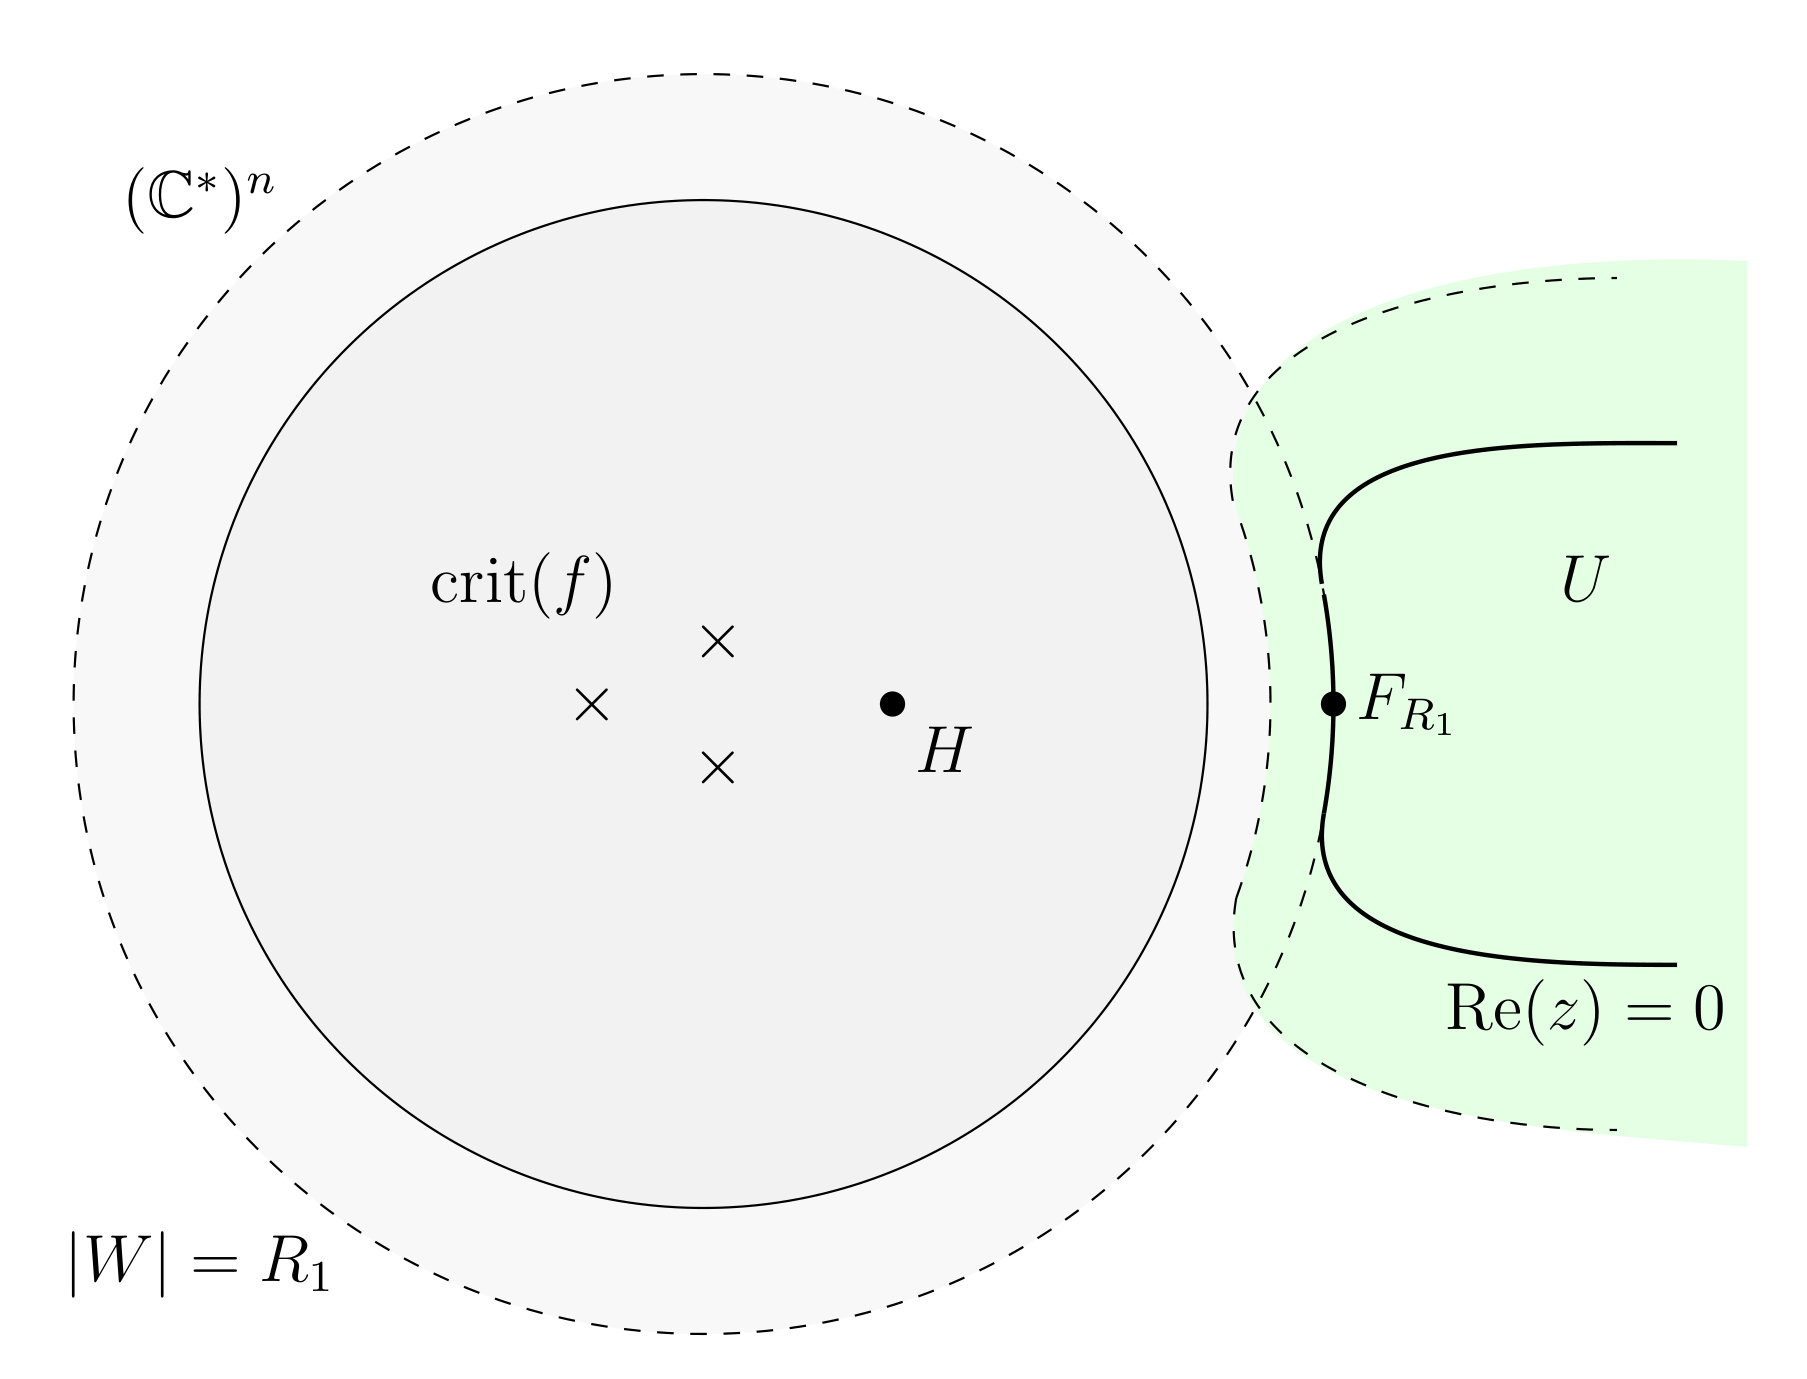
\includegraphics[width=0.56\textwidth]{figures/fig7_1.png}
\caption{命题 \ref{prop:7-1-1} 的证明：$U$（绿色）是纤维 $F_{R_1}$（黑点）的乘积邻域。}
\label{fig:7-1}
\end{figure}

$U$ 在完备化 $(\C^*)^n$ 中真嵌入。这里我们重申 $F_{R_1}$ 与 $H$ 的等同方式：沿一条射线作平行移动。于是扇形超曲面 $\{\operatorname{Re}(z)=0\}$ 把 $(\C^*)^n$ 表示成沿 $H$ 把 $(H\times\C,z)$ 粘到 $((\C^*)^n,f)$ 的扇形粘合（见图 \ref{fig:7-1}）。

接下来，我们在 $H\times\{z\in\C:\operatorname{Re}(z)>-\rho\}\setminus\{\rho\}$ 上引入一个 Liouville 形式，使它与原 Liouville 形式之差支撑在 $H\times\{\rho\}$ 的一个小开邻域上，做法如 [Jef22, Proposition 6]。此时超曲面 $\{\operatorname{Re}(z)=0\}$ 在无穷远处仍平行于 Liouville 向量场，于是可以把 $H\times\{z\in\C:\operatorname{Re}(z)>-\rho\}\setminus\{\rho\}$ 沿 $H$ 粘回一个与 $((\C^*)^n,f)$ 典范等同的扇形。另一方面，$(\C^*)^n$ 内存在 Liouville 超曲面的同痕，把 $H\times\{\rho\}$ 移到 $f^{-1}(0)$。

% ===== 原书 p.100 =====
\begin{figure}[htbp]
\centering
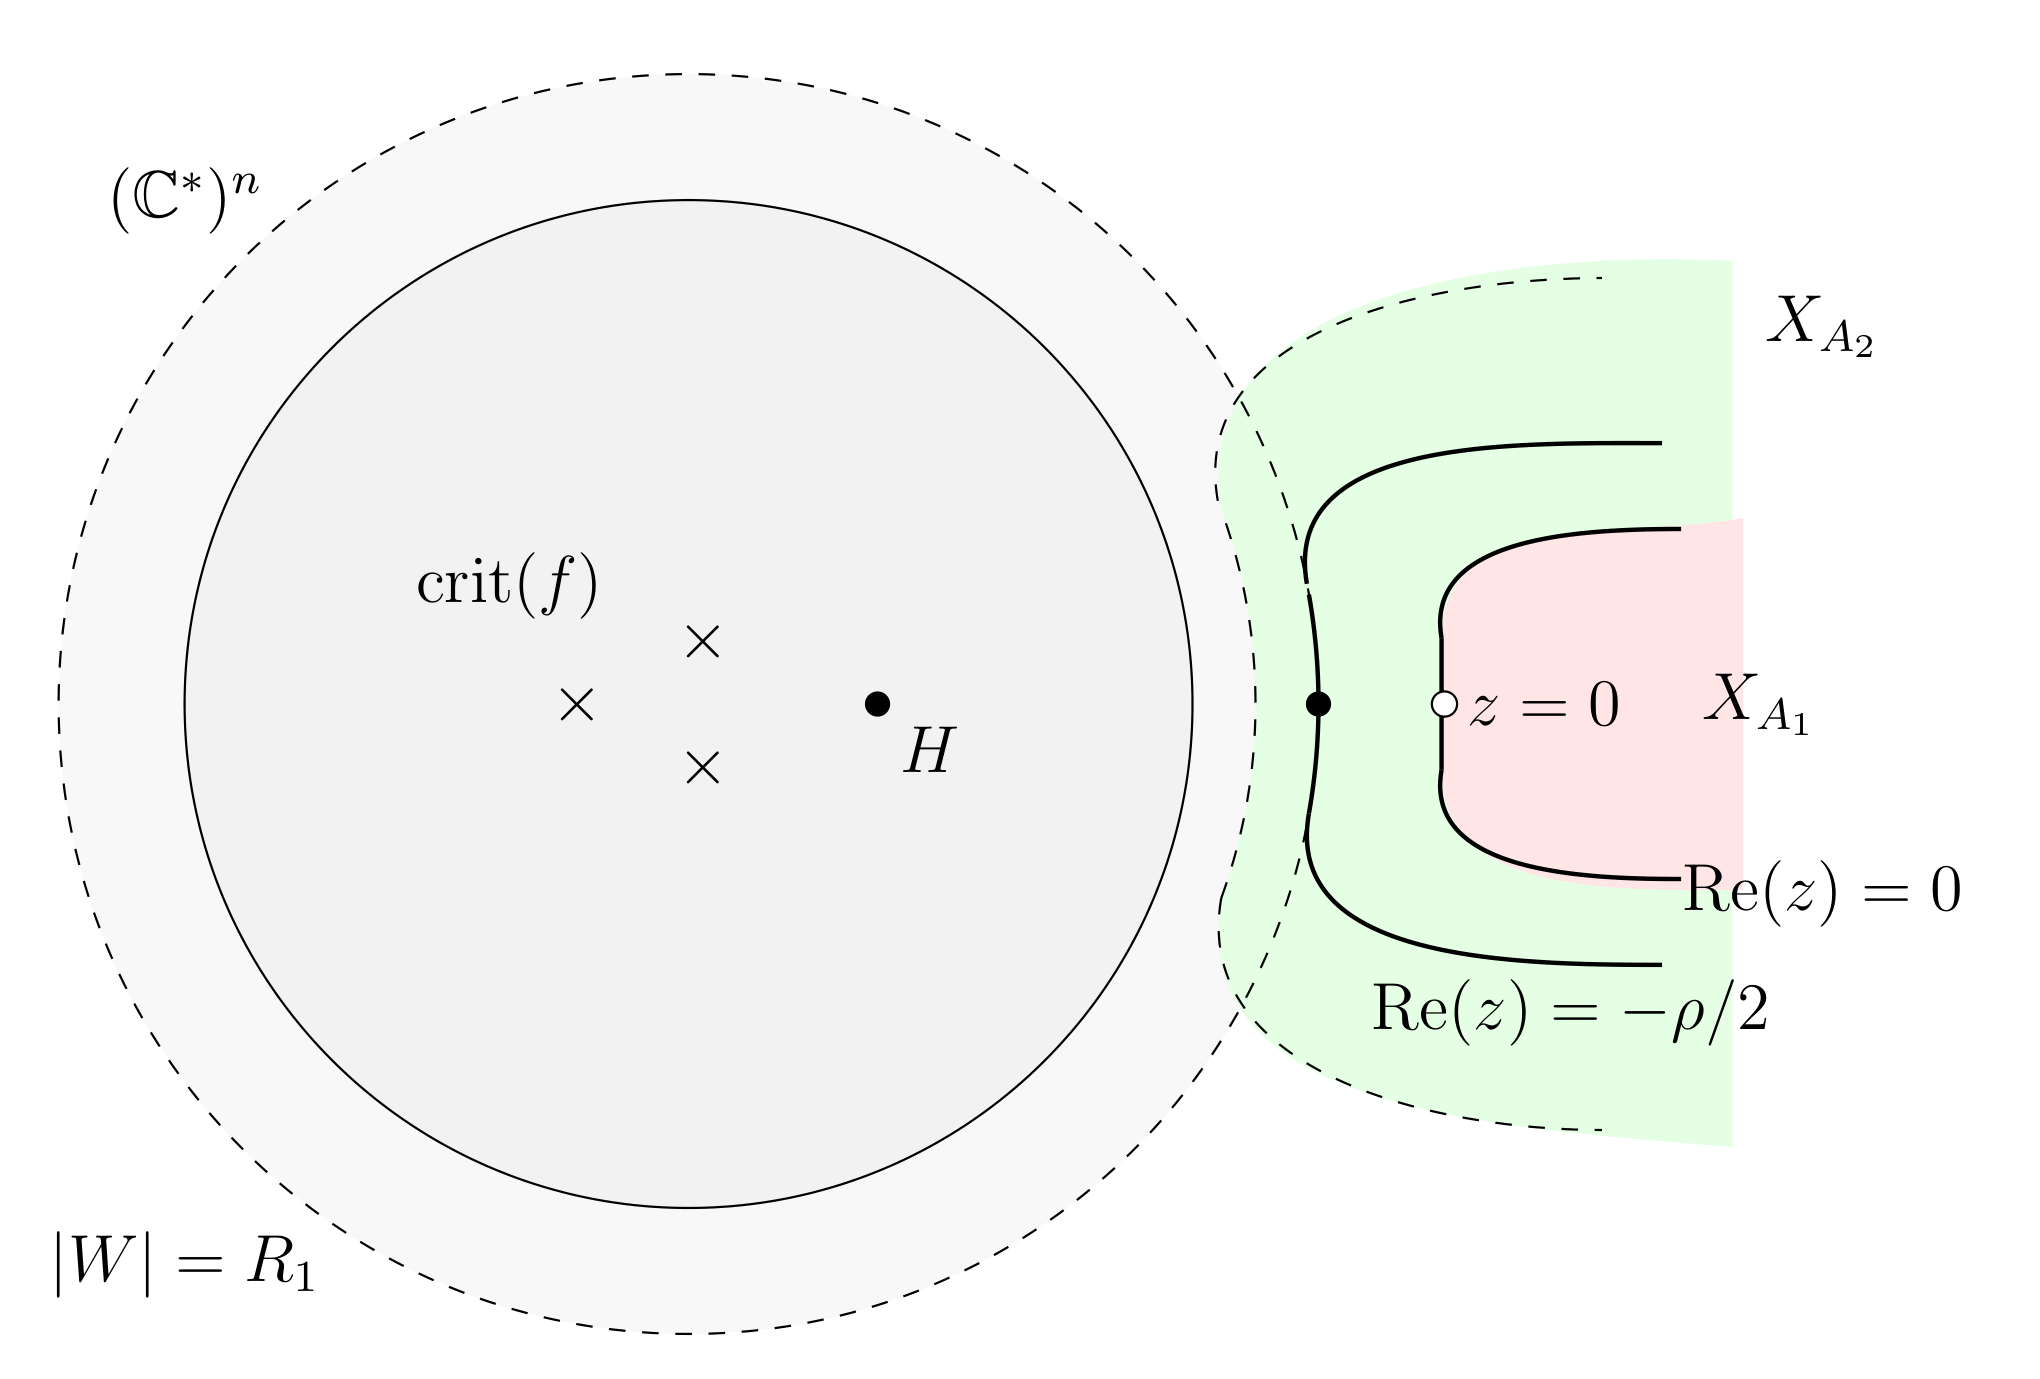
\includegraphics[width=0.64\textwidth]{figures/fig7_2.png}
\caption{命题 \ref{prop:7-1-2} 的证明：$X_{A_2}$ 为绿色，$X_{A_1}$ 为红色。}
\label{fig:7-2}
\end{figure}

于是应用 Moser 引理可知，这一粘合的结果与 $(\C^*)^n\setminus H$ 上的 Liouville 形式之间存在简单 Liouville 同伦；后者如 [Jef22] 所述，又与由限制得到的 $(\C^*)^n\setminus H\subseteq(\C^*)^{n+1}$ 上的原 Liouville 形式简单 Liouville 同伦。这就说明：沿 $H$ 把 $(H\times\C^*,z)$ 粘到 $((\C^*)^n,f)$ 所得的结果，同伦之后正是 $(\C^*)^n\setminus H$：见图 \ref{fig:7-2}。
\end{proof}

\transnote{易错预警：$F_{R_1}$ 与 $H$ 的等同依赖“沿一条射线作平行移动”这一选择，换一条射线会给出不同的等同；后文所有粘合映射都相对于这个选择。}

\transnote{含糊点拨：此处的 $z$ 是邻域 $U$ 上的坐标，它与原来的映射 $f$ 并不同；$z$ 的纤维只与 $f$ 的纤维同痕。原书在 p.99 明言这一点，读图 \ref{fig:7-1} 时容易误以为 $z=f$。}

\begin{remarkx}\label{rem:9}
我们应把这一分解看成与表示 $\tilde f_0=0$ 相联系的 $(\C^*)^n\setminus H$ 的扇形分解。
\end{remarkx}

\transnote{易错预警：$\tilde f_0$ 不是 $f$ 本身，而是 §2 中把 $0$ 处的单值性整理到无穷远之后得到的函数；两种表示 $\tilde f_0=0$ 与 $\tilde f_\infty=0$ 对应同一个 $(\C^*)^n\setminus H$，但扇形分解不同。}

回忆 [GPS19] 中的 $A_n$ 扇形：其定义是沿边界带 $n+1$ 个停点的标准 Liouville 圆盘 $D^2$。

\begin{proposition}\label{prop:7-1-2}
Liouville 流形 $(\C^*)^n\setminus H$ 简单 Liouville 同伦于如下扇形粘合：沿一条纤维 $H$ 把 $((\C^*)^n,f)$ 粘到扇形 $(E,H)$，而 $(E,H)$ 由 $H\times A_2$ 与 $H\times A_1$ 沿两个边界分支、通过等同 $\id\colon H\to H$ 与 $\mu\colon H\to H$ 粘合给出。
\end{proposition}

% ===== 原书 p.101 =====
\begin{figure}[htbp]
\centering
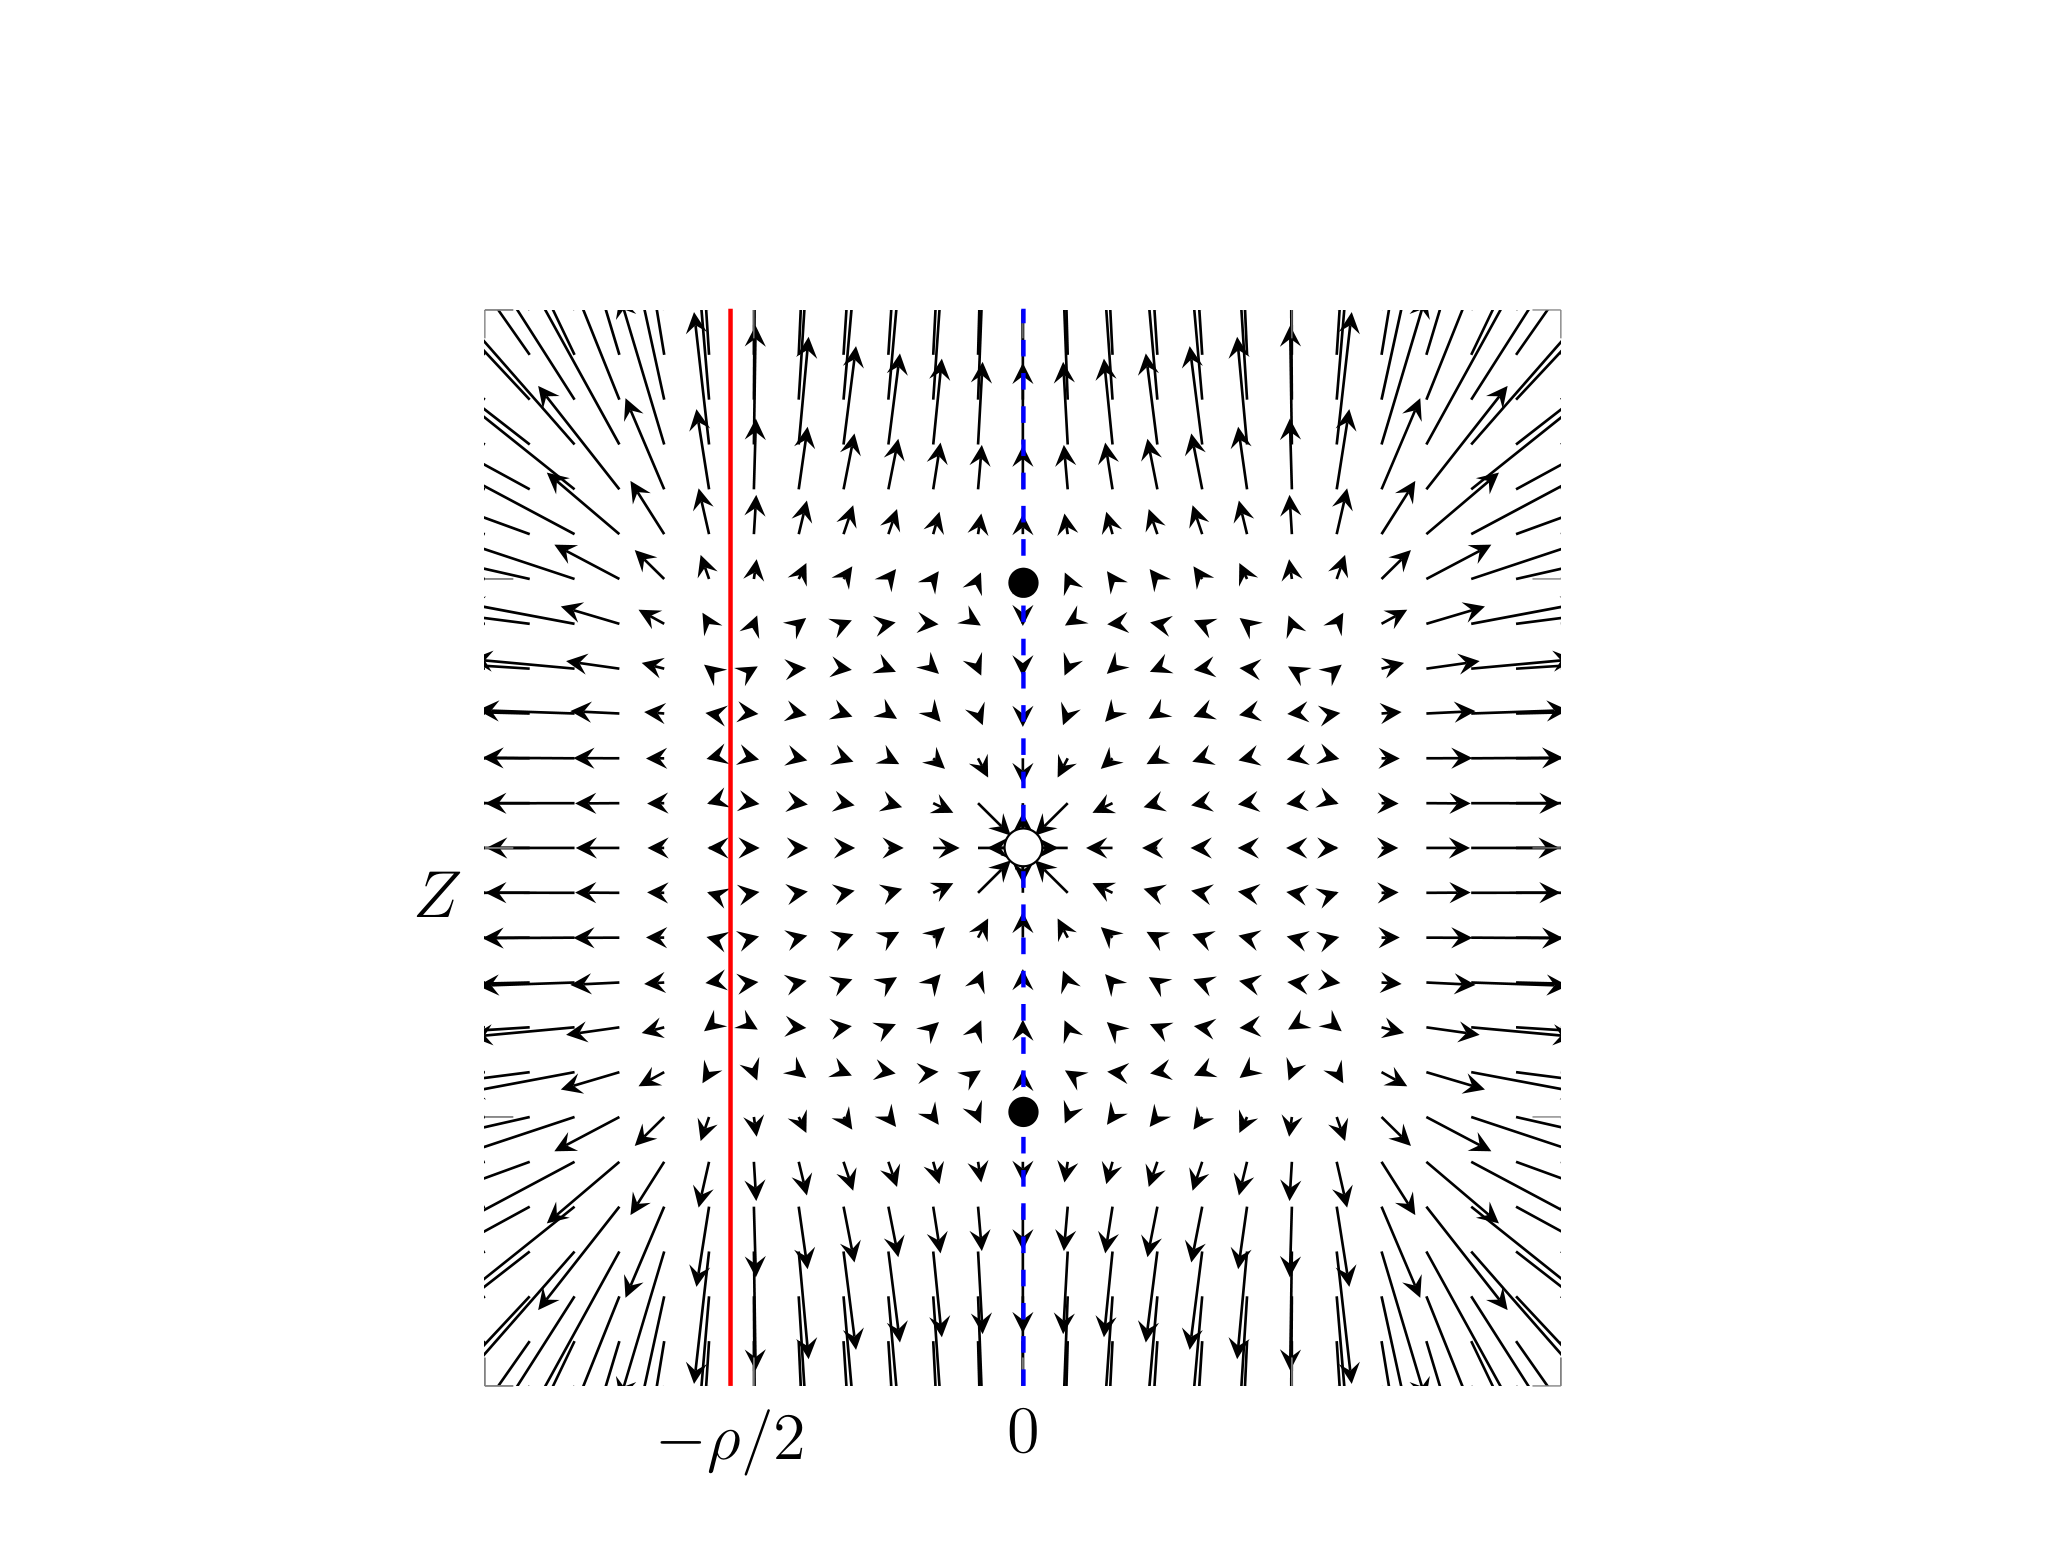
\includegraphics[width=0.52\textwidth]{figures/fig7_3.png}
\caption{命题 \ref{prop:7-1-2} 证明中形变后的 Liouville 向量场草图：超曲面 $\operatorname{Re}(z)=-\rho/2$ 为红色，两个黑点是 Liouville 向量场的零点。}
\label{fig:7-3}
\end{figure}

\begin{proof}
我们把证明拆成四步。先指出：若假定 $f$ 诱导出 $(\C^*)^n$ 边界的一个开书分解（open book decomposition），如 [GPS20a, Example 2.20] 所设，则论证可以大为简化。读者也可对照 [Gam20, Proposition 3.7]。

\transnote{含糊点拨：原文把“开书分解”当作可使论证大幅简化的额外假设，而未假定它成立；本证明不使用开书分解，只把这一情形作为对照。}

\begin{enumerate}
\item 设想延续上文命题 \ref{prop:7-1-1} 的论证：在邻域 $H\times\{z\in\C:\operatorname{Re}(z)>-\rho\}\setminus\{0\}$ 上存在显式的 Liouville 结构简单同伦，使 $\{\operatorname{Re}(z)=0\}$ 与 $\{\operatorname{Re}(z)=-\rho/2\}$ 都在无穷远处平行于 Liouville 向量场，并且仍以 $I=\operatorname{Im}(z)$ 作为 $I$-函数。所得 Liouville 向量场 $Z$ 的草图见图 \ref{fig:7-3}：它在 $\C^*$ 上处处有正散度，因而在彼处定义一个 Liouville 形式。这把 $(\C^*)^n\setminus H$ 表示成 $((\C^*)^n,f)$ 到两个扇形 $X_{A_2}\cong H\times A_2$ 与 $X_{A_1}\cong H\times A_1$ 的扇形粘合，粘合沿边界分支 $\partial(X_{A_2})$（它同痕于 $H\times\R$）进行（见图 \ref{fig:7-2}）。

% ===== 原书 p.102 =====
\begin{figure}[htbp]
\centering
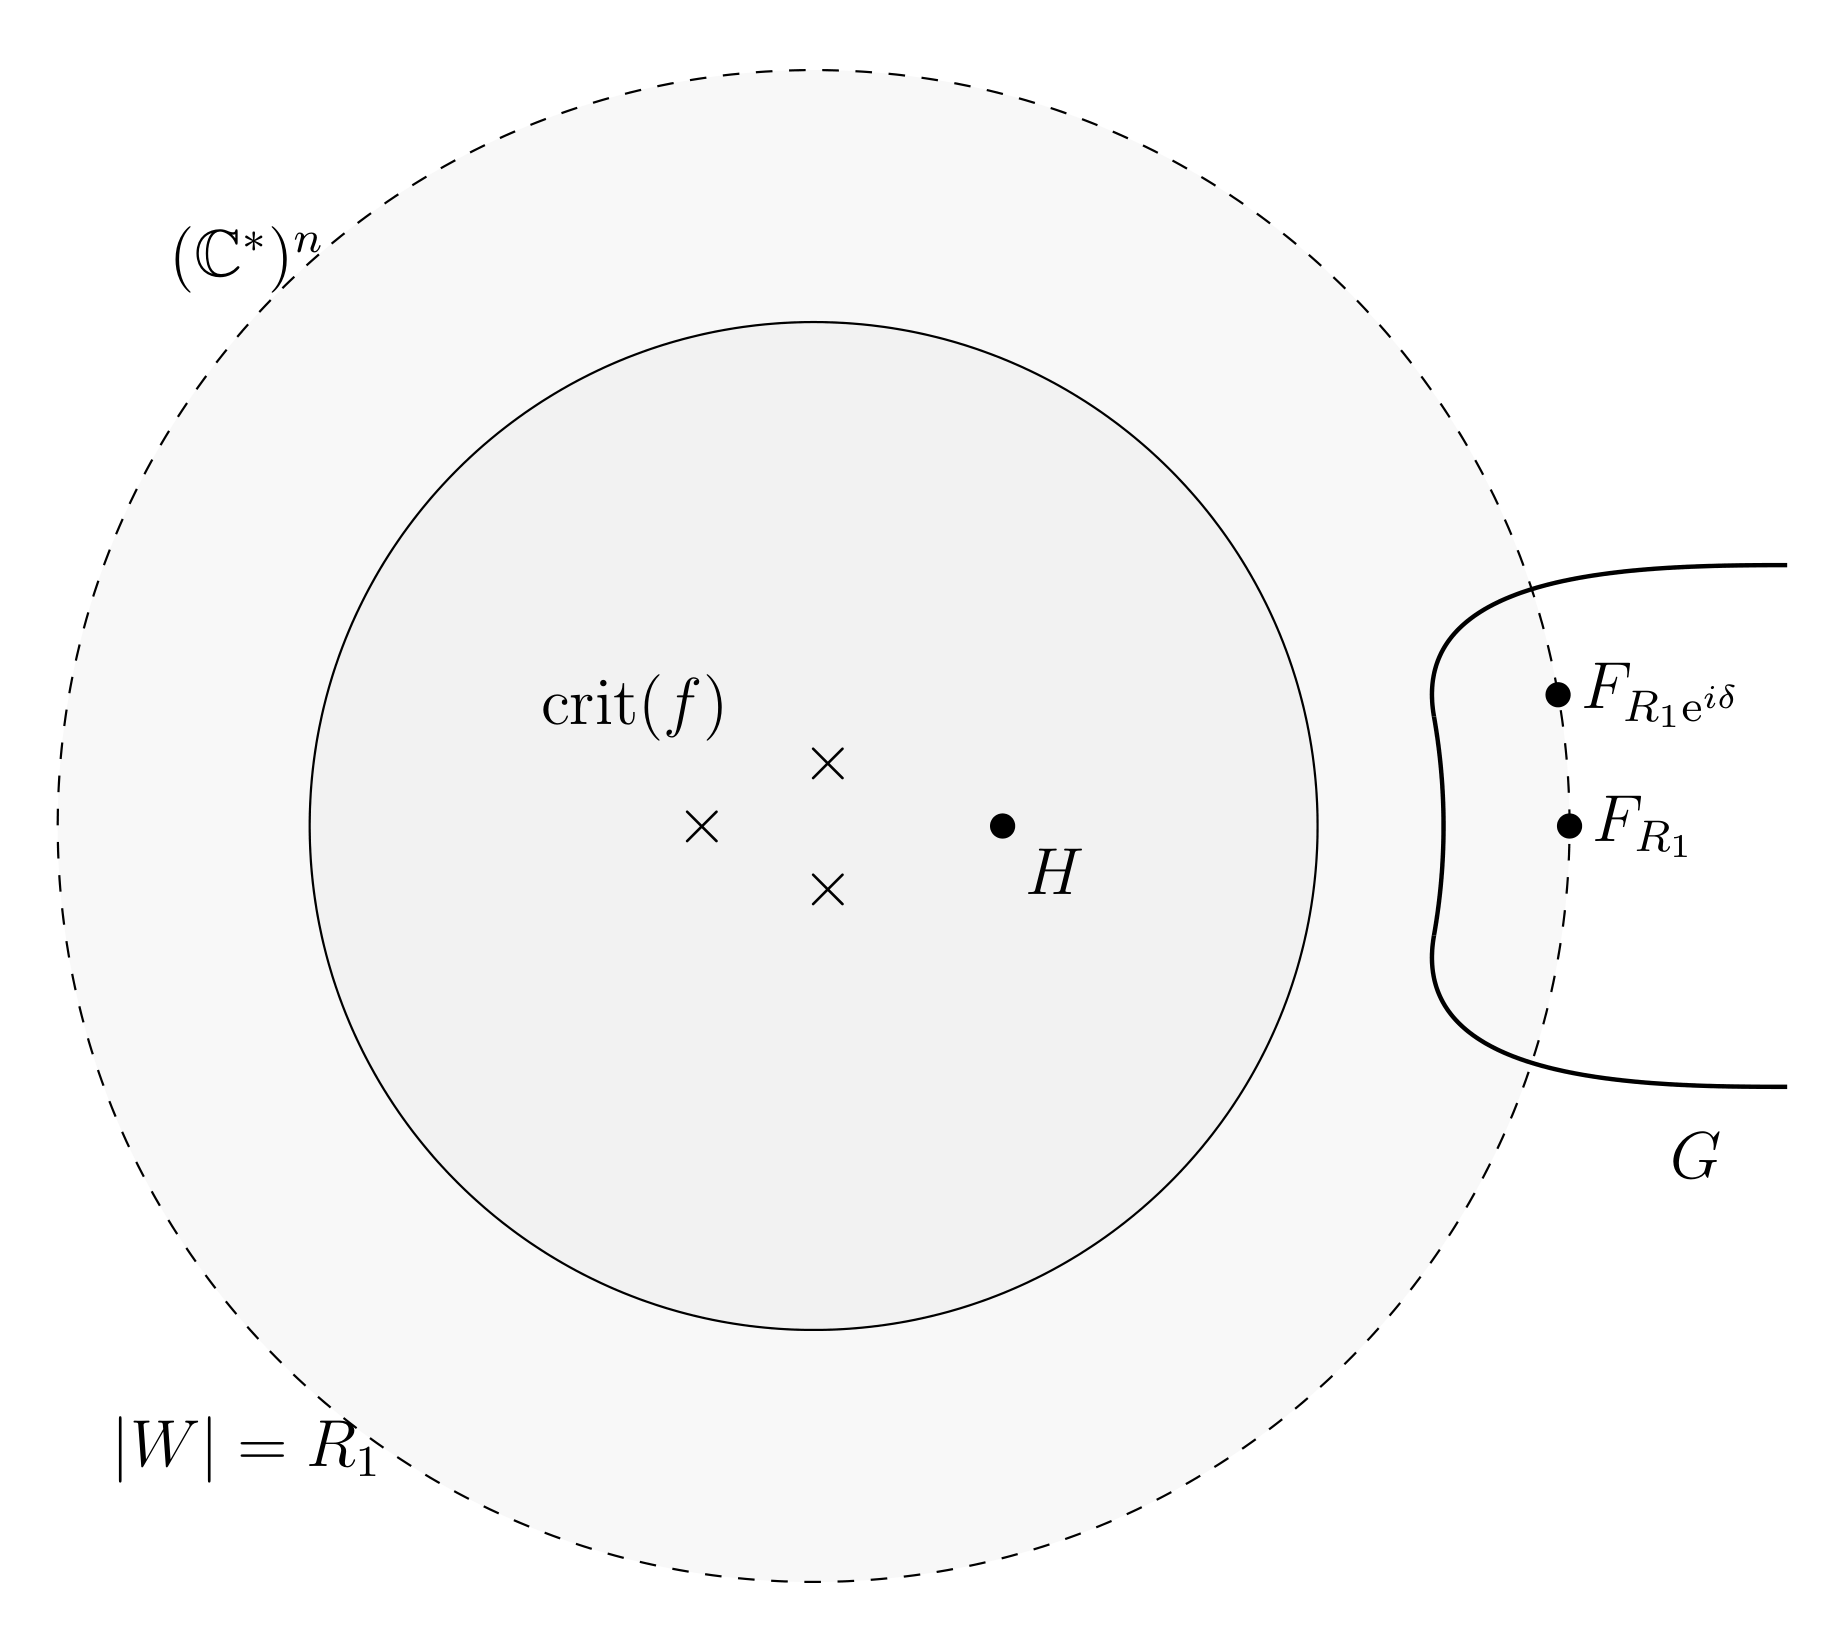
\includegraphics[width=0.54\textwidth]{figures/fig7_4.png}
\caption{命题 \ref{prop:7-1-2} 的证明：超曲面 $F_{R_1e^{i\delta}}$、$F_{R_1}$ 与扇形超曲面 $G$。}
\label{fig:7-4}
\end{figure}

% ===== 原书 p.103 =====
\begin{figure}[htbp]
\centering
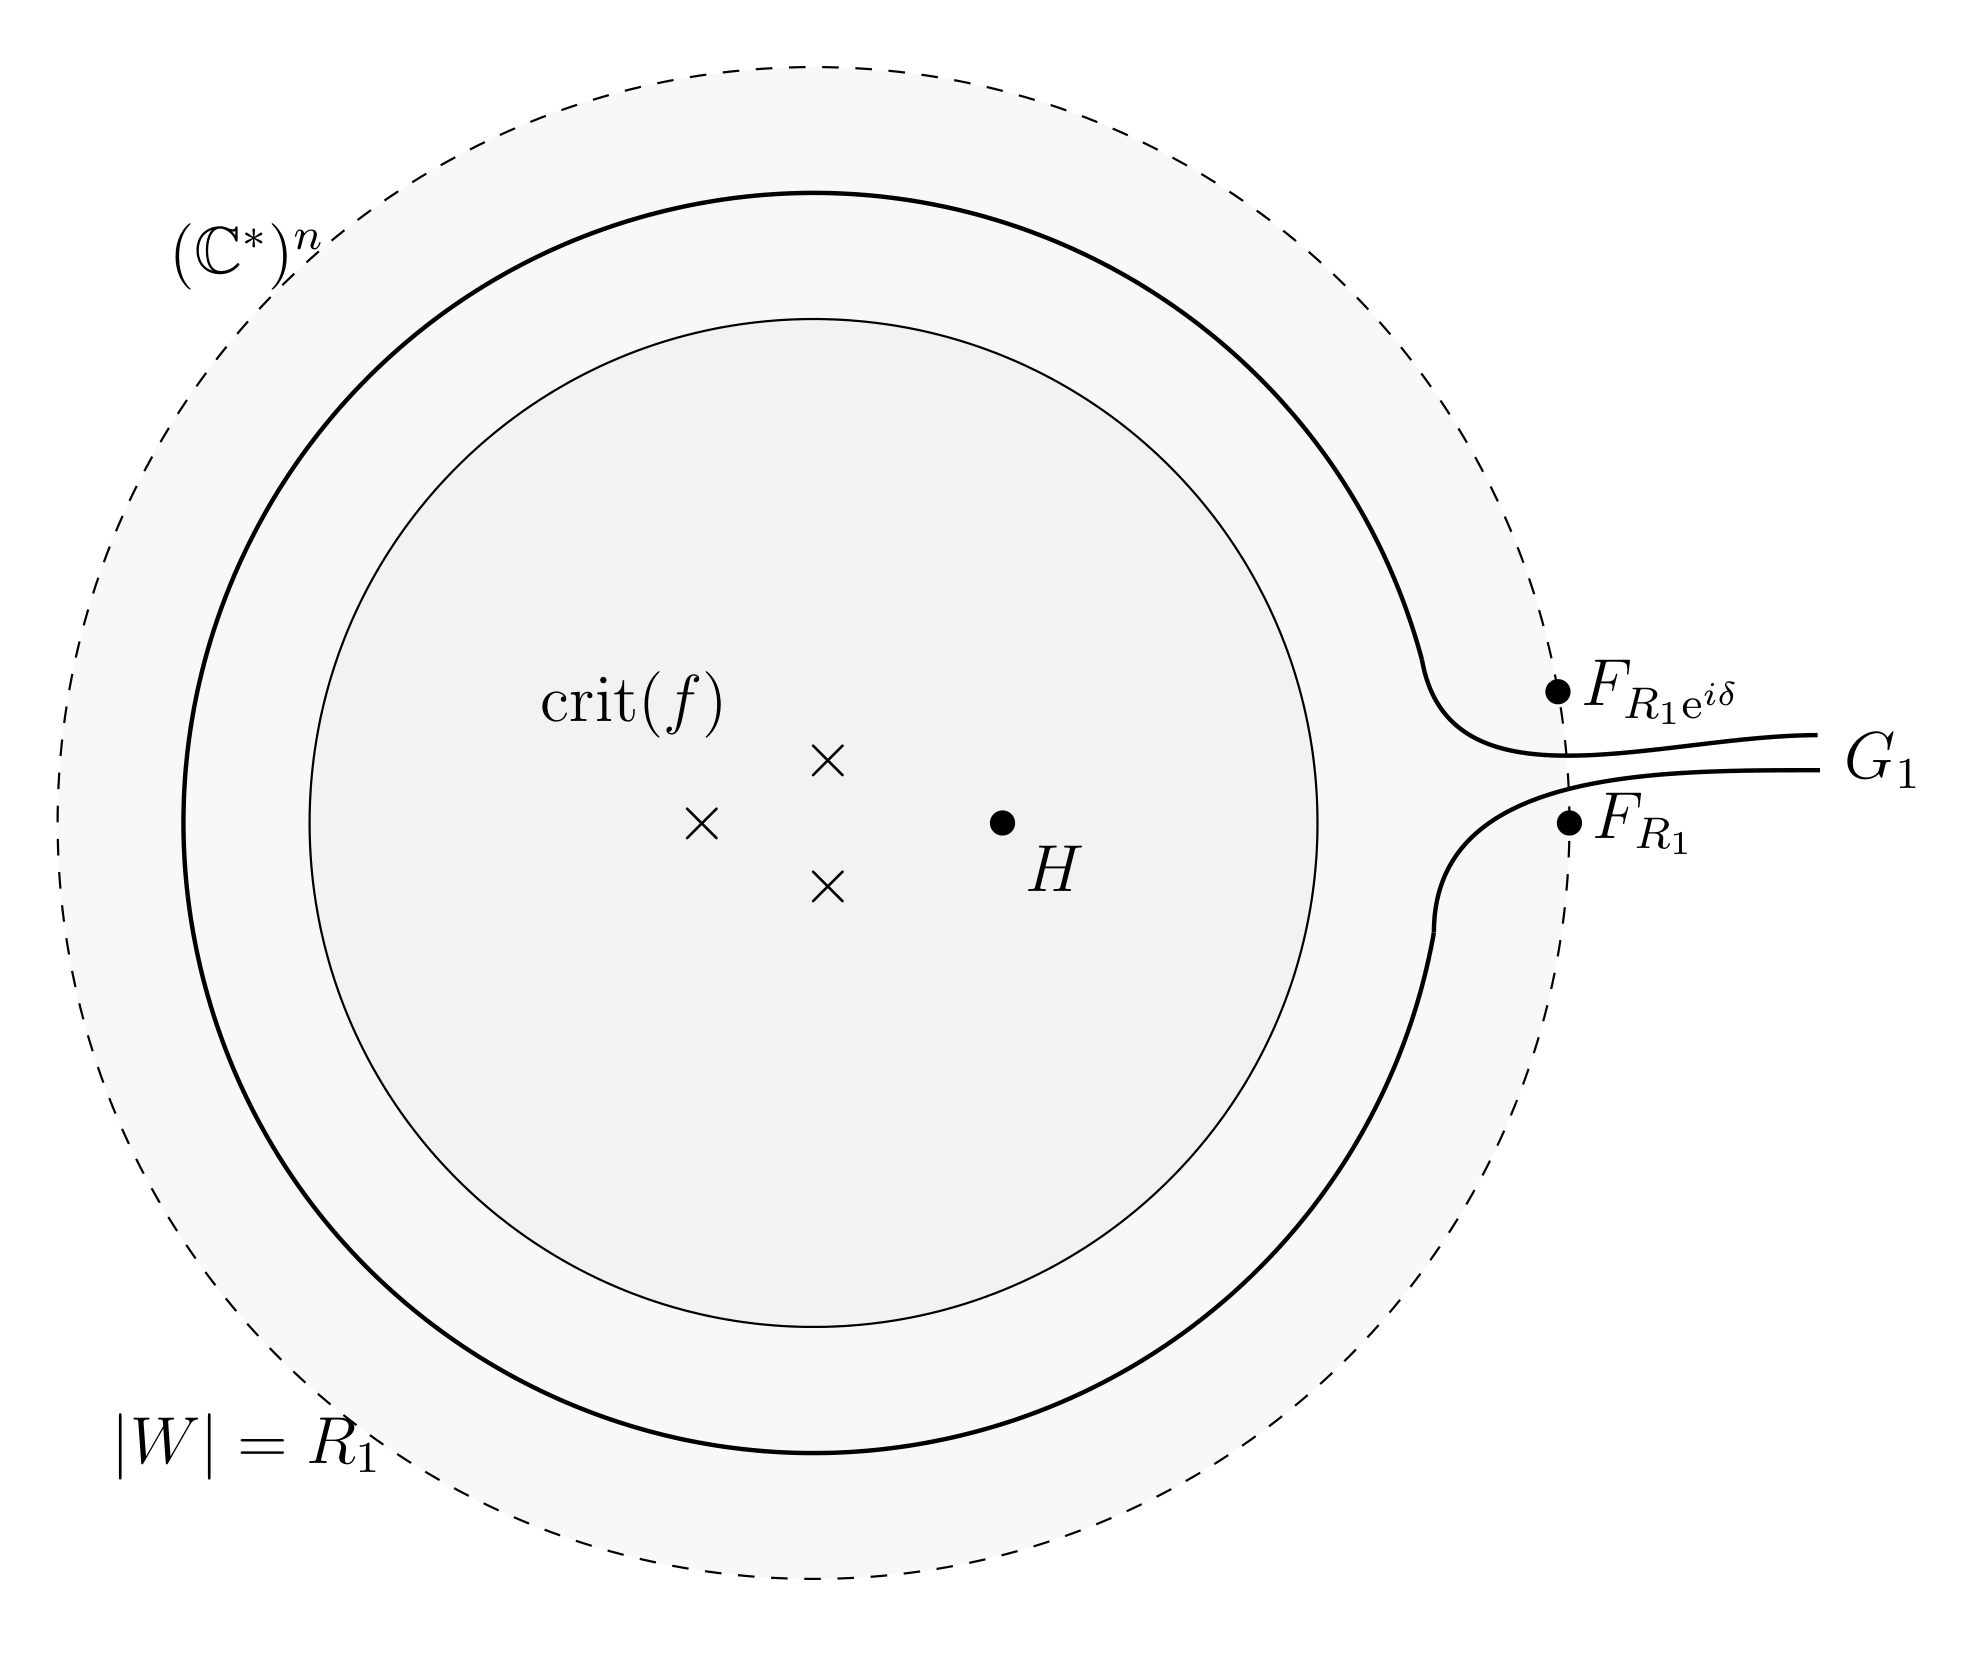
\includegraphics[width=0.54\textwidth]{figures/fig7_5.png}
\caption{命题 \ref{prop:7-1-2} 的证明：施加以 $F_{R_1e^{i\delta}}$ 与 $F_{R_1}$ 互换的同痕之后，扇形超曲面 $G$ 的像 $G_1$。}
\label{fig:7-5}
\end{figure}

% ===== 原书 p.104 =====
\item 作与 [Jef22, Proposition 6] 类似的论证：施加一个把被去掉的纤维移到无穷远的同痕，再应用 [GPS20a, Lemma 2.32] 的唯一性结果，可以证明 Liouville 扇形 $X_0=(\C^*)^n\cap\{\operatorname{Re}(z)\le0\}$ Liouville 同伦于如下结果：把 [Syl19b, Proposition 2.6] 应用于 Liouville 区域 $(\C^*)^n_0=\{|W|\le R_1\}\cap\{\psi\le R_2\}$，沿一对 Liouville 超曲面 $F=|W|^{-1}\bigl(\{R_1,R_1e^{i\delta}\}\bigr)\cap\{\psi\le R_2-\eps\}$ 切开。这里我们经 $\Phi_\eta$ 等同 $F_{R_1e^{i\delta}}$ 与 $F_{R_1}$。

等价地，取双覆盖 $q\colon\C\to\C$，使 $q(z)=c$ 的两个根在 $c$ 绕单位圆一周时描出曲线 $\gamma$ 与 $\eta(t)=e^{it\delta}$。令 $\tilde f(x)=q(1-f(x))$，则 Liouville 扇形 $(\C^*)^n\cap\{\operatorname{Re}(z)\le0\}\setminus\{0\}$ Liouville 同伦于：把 [Syl19b, Proposition 2.6] 应用于 Liouville 区域 $(\C^*)^n_0$ 与超曲面 $F=\tilde f^{-1}(1)\cap\{\phi\le R_2-\eps\}$ 的结果。

\transnote{易错预警：$(\C^*)^n_0$ 的下标 $0$ 指“取 $|W|\le R_1$ 截断后的区域”，与 $\eta_0$、$\alpha_0$、$\cW_0$ 的下标 $0$ 无关，切勿混为一谈。}

\item 由 [GPS20a, Lemma 2.32] 的同伦唯一性，取 Liouville 超曲面的同痕 $\widetilde F_t=\tilde f^{-1}(e^{2\pi it})$（$t\in[0,1]$），给出相应 Liouville 扇形 $X_t$ 的唯一 Liouville 同伦。扇形边界 $\partial X_1$ 的两个分支经 Liouville 流回缩（对应图 \ref{fig:7-3} 中标出的两个黑点）之后，与 $F_{R_1e^{i\delta}}\times\R$ 及 $F_{R_1}\times\R$ 典范等同。

此外，扇形超曲面 $G=\{\operatorname{Re}(z)=-\rho/2\}\subseteq X_0$ 会在该同伦下变为扇形超曲面 $G_t\subseteq X_t$，并在无穷远处保持平行于 Liouville 向量场：见图 \ref{fig:7-4}。这个扇形超曲面把 $X_t$ 表示成两个扇形的粘合；由唯一性引理，第一个 Liouville 同伦于 $((\C^*)^n,f)$，第二个 $X^t_{A_2}$ 同伦于 $H\times A_2$（见图 \ref{fig:7-6}）。

\transnote{含糊点拨：原文说 $X^t_{A_2}$ “同伦于 $H\times A_2$”，指 Liouville 同伦而非辛同胚；扇形 $X^t_{A_2}$ 随 $t$ 变动，只有同伦类保持不变。}

% ===== 原书 p.105 =====
\item 最后，把扇形 $H\times A_1$ 沿 $\partial X_1$ 粘到 $X_1$ 所得的结果，是一个 Liouville 同伦于 $(\C^*)^n\setminus H$ 的 Liouville 流形（见图 \ref{fig:7-6}）。我们来理解这一粘合涉及的等同。Liouville 同痕 $\widetilde F_t$ 给出辛同胚 $\Phi_\gamma\colon F_{R_1}\to H$ 与 $\Phi_\eta\colon F_{R_1e^{i\delta}}\to H$，它们把边界 $\partial X_1$ 表示成 $(H\times\R)\sqcup(H\times\R)$。

在原来的表示 $X_0$ 中，我们把 $X_{A_1}$ 粘到 $X_{A_2}$ 得到 $(\C^*)^n\setminus H$。回忆纤维 $F_{R_1}$ 经沿一条射线的平行移动与参考纤维 $H$ 等同。这条纤维 $F_{R_1}$ 是 [Syl19b, Proposition 2.6] 的形变之后 Liouville 流的源头，故 $((\C^*)^n,f)$、$X_{A_2}$ 与 $X_{A_1}$ 的扇形边界的每个分支都典范等同于 $F_{R_1}\times\R$。

于是，用原来的粘合映射 $\id\colon F_{R_1}\to F_{R_1}$ 与 $\Phi_\eta\colon F_{R_1}\to F_{R_1e^{i\delta}}$ 把 $X_{A_1}$ 粘回 $X_1$，再与我们已有的与 $H$ 的等同复合，就得到粘合映射 $\mu\colon H\to H$ 与 $\Phi_\eta\colon H\to H$（后者同痕于恒等）。这就完成了论断的证明。
\end{enumerate}
\end{proof}

\transnote{易错预警：此处的 $\mu\colon H\to H$ 是辛同胚（几何单值性），不是第 8 章讨论的单值函子 $\mu\colon\cW(H)\to\cW(H)$，也不是前面带停点范畴里的 $\mu$ 单子；同名不同物。}

\begin{remarkx}\label{rem:10}
我们应把这一分解看成与表示 $\tilde f_\infty=0$ 相联系的 $(\C^*)^n\setminus H$ 的扇形分解。此时改用 $-1/f$ 给出的投影 $(\C^*)^n\setminus H\to\C$。其效果是交换 $0$ 与 $\infty$：$f$ 的全部单值性现在都围绕 $0\in\C^*$ 发生。
\end{remarkx}

相应地，我们本想用超曲面 $\operatorname{Re}(1/f)=1/2$ 把 $(\C^*)^n\setminus H$ 切成两个扇形。技术细节使这一点难以实行，所以我们改用命题 \ref{prop:7-1-2} 给出的论证，得到一种等价的扇形粘合表示。第二作者与合作者未来的工作将去掉对这一论证的需要。

\transnote{背景直觉：把 $f$ 换成 $-1/f$ 是“交换零与无穷”的标准手法：$f$ 的奇异纤维位于 $0$ 上方，$-1/f$ 的奇异纤维则跑到无穷远，同时单值性挪到 $0\in\C^*$ 附近。}

\begin{definition}\label{def:7-1-3}
给定上述扇形分解，我们定义：
\begin{enumerate}
\item 函子 $\alpha_\infty\colon\cW((\C^*)^n,f)\to\cW((\C^*)^n\setminus H)$ 由命题 \ref{prop:7-1-1} 中的扇形包含给出；
\item 函子 $\alpha_0\colon\cW((\C^*)^n,f)\to\cW((\C^*)^n\setminus H)$ 由命题 \ref{prop:7-1-2} 中的扇形包含给出。
\end{enumerate}
\end{definition}

% ===== 原书 p.106 =====
\begin{figure}[htbp]
\centering
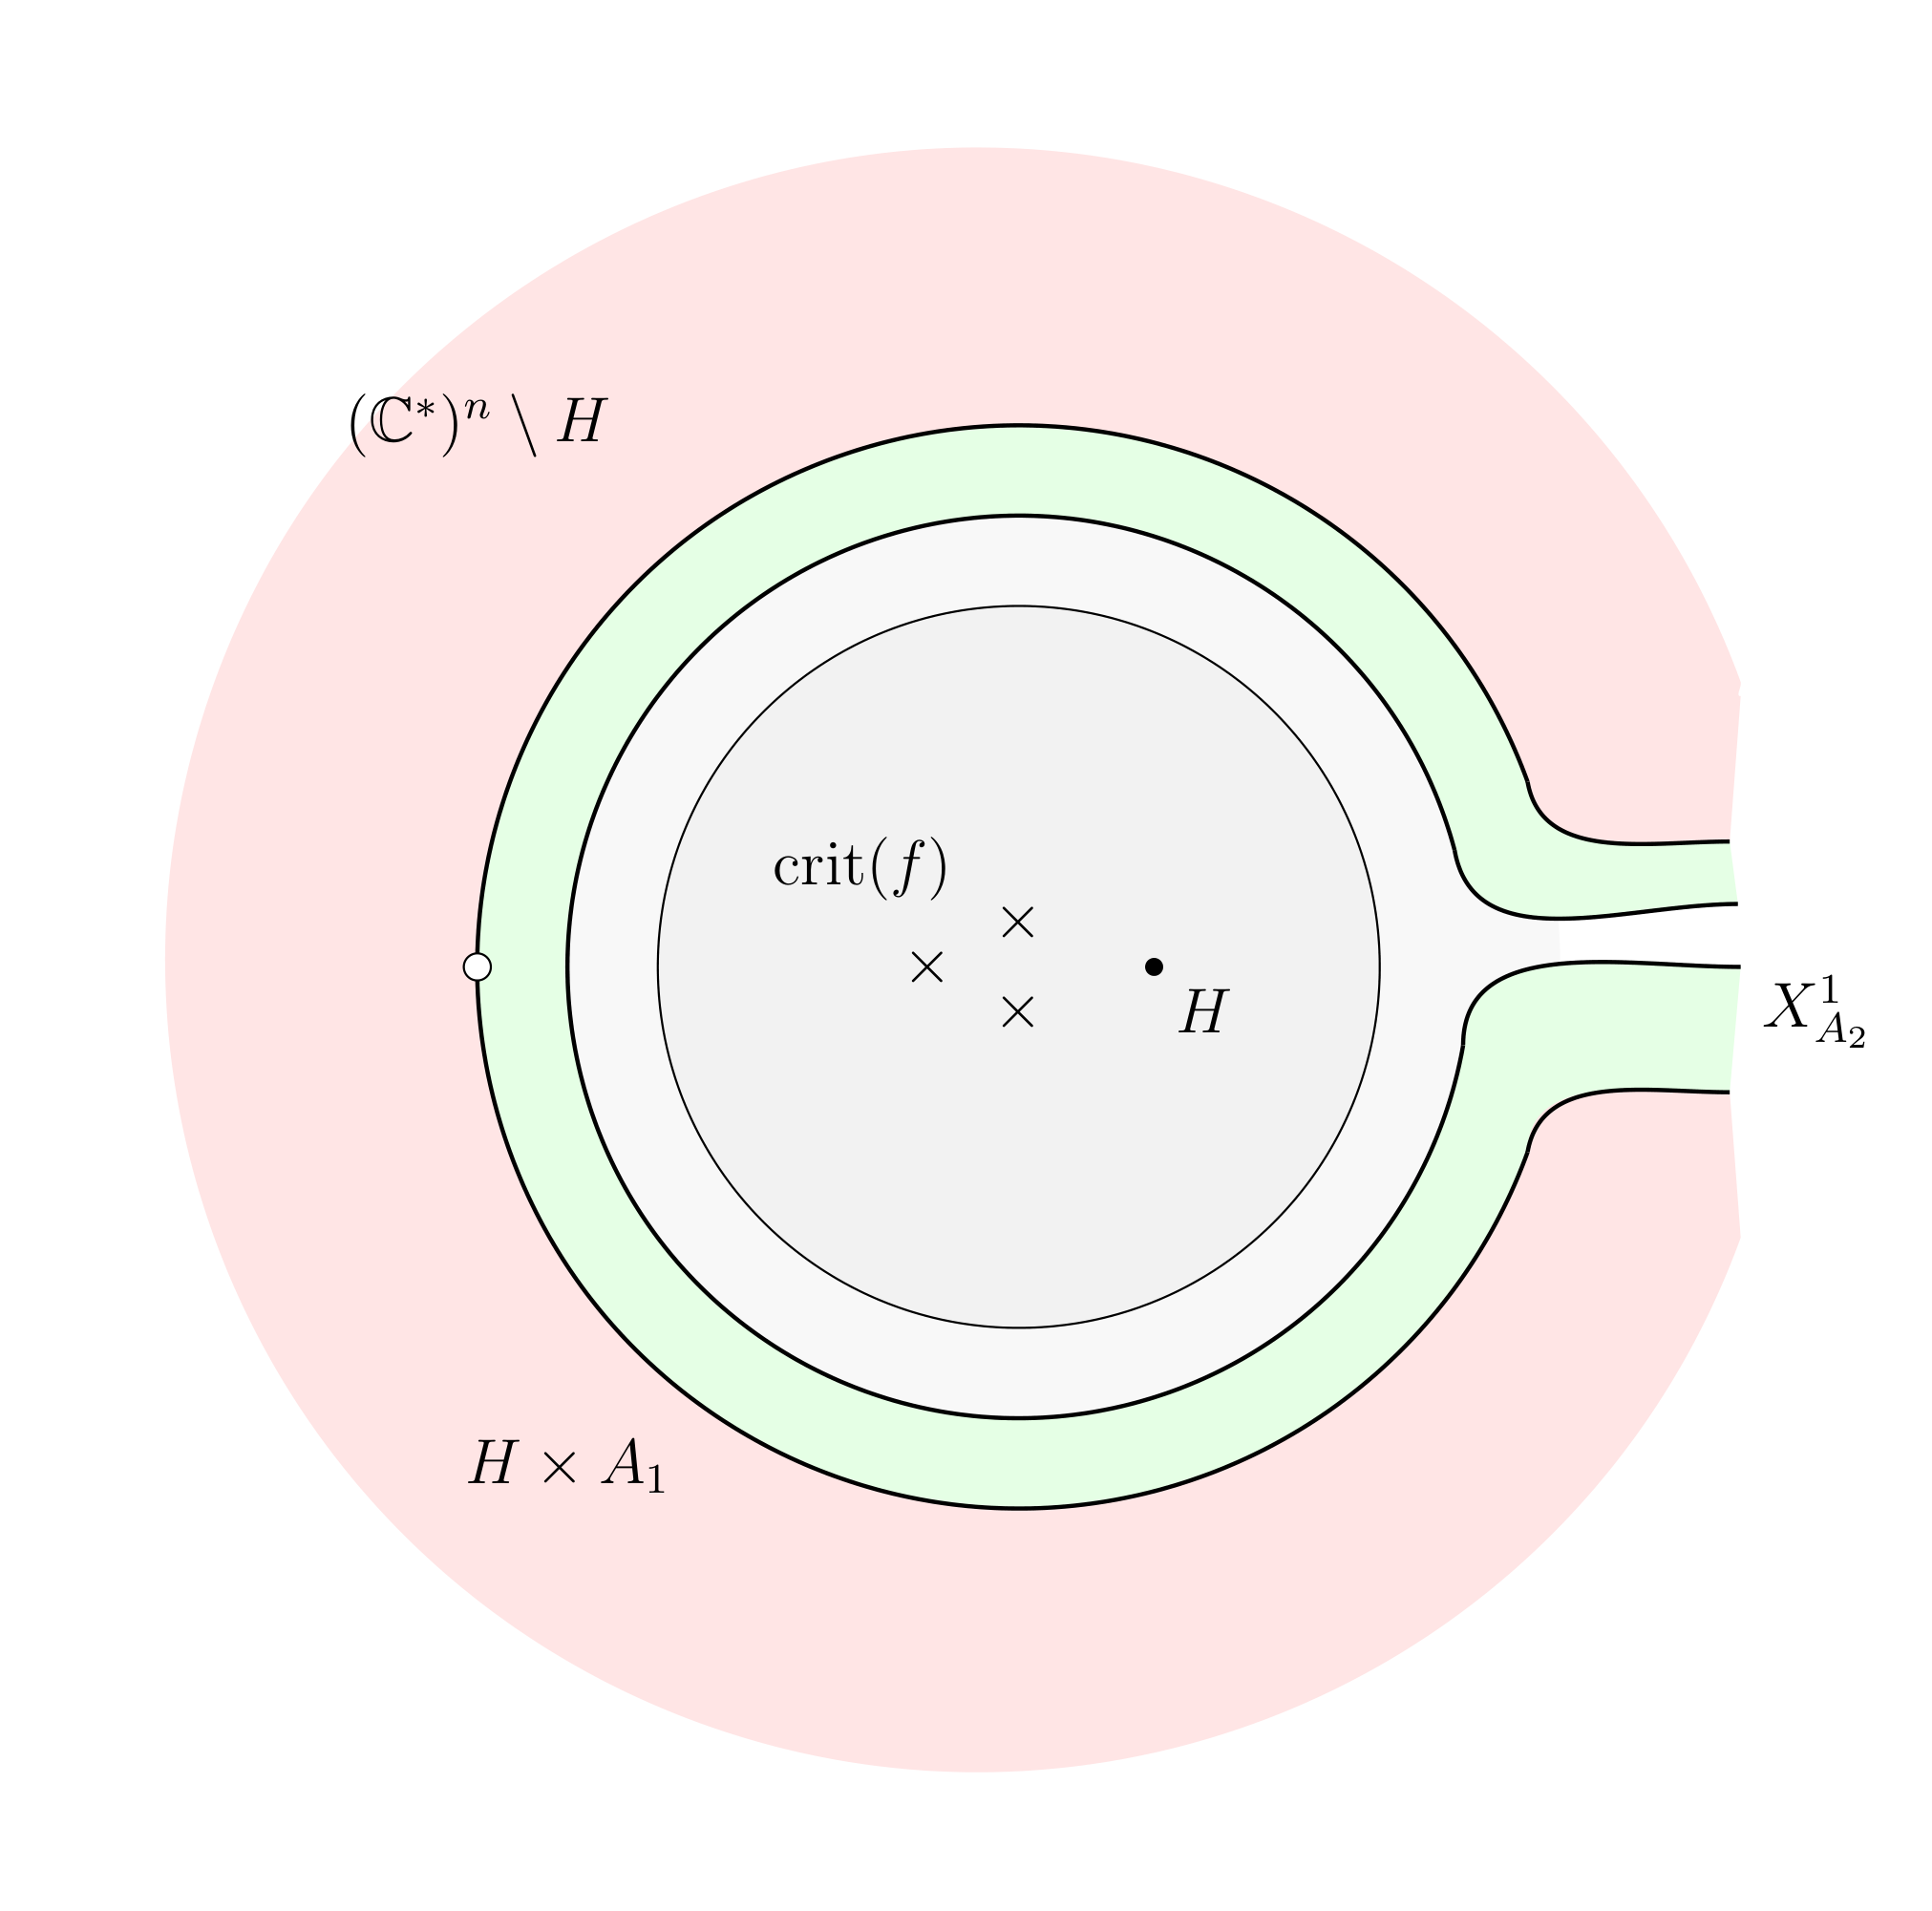
\includegraphics[width=0.55\textwidth]{figures/fig7_6.png}
\caption{命题 \ref{prop:7-1-2} 的证明：扇形 $X^1_{A_2}$ 为绿色，扇形 $H\times A_1$ 为红色。}
\label{fig:7-6}
\end{figure}

% ===== 原书 p.107 =====
\begin{corollary}\label{cor:7-1-4}
有 wrapped Fukaya 范畴的推出（pushout）图表：
\[
\begin{tikzcd}[column sep=3.0em, row sep=1.8em]
\cW(H) \arrow[r, "\cup"] \arrow[d] & \cW((\C^*)^n,f) \arrow[d, "\alpha_\infty"] \\
\cW(H\times\C^*(2),z) \arrow[r] & \cW_0((\C^*)^n\setminus H)
\end{tikzcd}
\qquad
\begin{tikzcd}[column sep=3.0em, row sep=1.8em]
\cW(H) \arrow[r, "\cup"] \arrow[d] & \cW((\C^*)^n,f) \arrow[d, "\alpha_0"] \\
\cW(E,z) \arrow[r] & \cW_\infty((\C^*)^n\setminus H)
\end{tikzcd}
\]
其中 $\cW(H\times\C^*(2),z)$ 记如下 wrapped Fukaya 范畴：简单逆时针 Reeb 轨道绕 $0$ 的次数为 $2$。
\end{corollary}

\transnote{易错预警：$\C^*(2)$ 里的 $(2)$ 是分次移位的信息，不是幂次，也不是“取两次”的记号；它表示绕 $0$ 的简单逆时针 Reeb 轨道的次数为 2。}

\begin{proof}
见 [GPS19, Theorem 1.28]：检查其论证可知，只要分次数据适当地粘合，那些论证可推广到 $\Z$-分次范畴（参 [GPS20c]）。注意 $\eta_0$ 由 $\eta_\infty$ 作上同调类 $[\arg(f)]$ 的扭得到；该上同调类限制到子扇形 $((\C^*)^n,f)$ 上平凡（因为 $f$ 在那里作为 Cartier 除子平凡），所以两个图表中可以使用同一个 $\Z$-分次范畴 $\cW((\C^*)^n,f)$。
\end{proof}

\begin{remarkx}\label{rem:11}
注意这些几何粘合结果与所选的分次结构无关；因此上面两个图既可以写成用 $\eta_0$-分次，也可以写成用 $\eta_\infty$-分次。
\end{remarkx}

\subsection{镜像对称}

\begin{proposition}\label{prop:7-2-1}
有交换图表：
\[
\begin{tikzcd}[column sep=4.4em, row sep=2.8em]
\cW(H) \arrow[r] \arrow[d, "\cup"'] & \operatorname{Coh}(D) \arrow[d, "i_{D*}"] \\
\cW((\C^*)^n,f) \arrow[r] & \operatorname{Coh}(X)
\end{tikzcd}
\]
其中横箭头是 [GS22; Kuw20] 给出的等价。此外，$f$ 绕 $\infty$ 的逆时针单值函子 $\mu\colon\cW(H)\to\cW(H)$ 镜像于 $\operatorname{Coh}(D)$ 上与反典范丛 $\cK_X^{-1}|_D$ 作张量。
\end{proposition}

\transnote{易错预警：原图在竖箭头旁另画弧形箭头，表示左伴随：$\cup$ 的左伴随是 $\cap$，$i_{D*}$ 的左伴随是 $i_D^*$。这两个伴随在证明中被用来把一侧的等价搬到另一侧，读图时不可略去。}

\begin{proof}
我们知道，在 [GS22] 的镜像对称等价下 $\cup$ 与 $i_{D*}$ 相对应（见 Figure 6）。因此它们的左伴随 $\cap^L$ 与 $i_D^*$ 也必定互为镜像。用反常束的语言说，球函子 $S$ 的对偶余扭（dual cotwist）由余单位映射 $S^LS\to\id$ 的锥给出，其中 $S^L$ 记左伴随。

[Syl19d, Theorem 1.3] 证明：$f$ 绕 $\infty$ 的几何逆时针单值性 $\mu$ 作用在 $\cW(H)$ 上时，等于 $\cup$ 的对偶余扭再平移 $[2]$。由 [Nad19b, p.12] 可知，$i_{D*}$ 的对偶余扭由 $\otimes\cK_X^{-1}|_D[-2]$ 给出。消去这两个 2-平移，即知函子 $\mu$ 对应于 $\otimes\cK_X^{-1}|_D$。
\end{proof}

\transnote{含糊点拨：原文作“见 Figure 6”，指原书第 6 章的图 6。本译注把第 6 章编为另一块，此处照原文字面译出，未加交叉引用。}

\begin{proposition}\label{prop:7-2-2}
$(E,H)$ 与 $K_X|_D$ 之间存在镜像对称等价，使得下图交换：
\[
\begin{tikzcd}[column sep=3.6em, row sep=2.2em]
\cW(H) \arrow[r] \arrow[d, "\cup"'] & \operatorname{Coh}(D) \arrow[d, "\iota_{D*}"] \\
\cW(E,z) \arrow[r] & \operatorname{Coh}(K_X|_D)
\end{tikzcd}
\]
其中顶部横箭头是 [GS22] 的等价。
\end{proposition}

% ===== 原书 p.108 =====
\begin{proof}
$K_X|_D$ 的全空间是 $D$ 上代数层 $\operatorname{Sym}(\cK_X^{-1}|_D)$ 的相对 Spec。于是全空间上的相干层范畴，由 $D$ 上带相干 $\operatorname{Sym}(\cK_X^{-1}|_D)$-模结构的拟相干层 $\mathcal F$ 构成的范畴给出。由 $\operatorname{Sym}$ 的泛性质，这样的数据等同于一个态射 $\mathcal F\otimes\cK_X^{-1}|_D\to\mathcal F$，它描述 $\operatorname{Sym}(\cK_X^{-1}|_D)$ 的生成元如何作用在 $\mathcal F$ 的截面上。

因此可以把 $\operatorname{Coh}(K_X|_D)$ 描述为如下对 $(\mathcal F,\varphi\colon\mathcal F\otimes\cK_X^{-1}|_D\to\mathcal F)$ 的范畴：$\mathcal F$ 是 $D$ 上的拟相干层，$\varphi$ 使 $\mathcal F$ 具有 $(\cdot\otimes\cK_X^{-1}|_D)$-单子上的有限生成模结构。参 [Gam20, Proposition 5.8]。推前函子 $\operatorname{Coh}(D)\to\operatorname{Coh}(K_X|_D)$ 只是把层 $\mathcal F$ 送到平凡作用 $\mathcal F\otimes\cK_X^{-1}|_D\to\mathcal F$。

\transnote{含糊点拨：“相对 Spec”指把 $\operatorname{Sym}(\cK_X^{-1}|_D)$ 看作 $D$ 上的拟凝聚代数层，再取它在 $D$ 上的相对谱；$K_X|_D$ 作为 $D$ 上的线丛，其全空间正是这个相对 Spec。}

% ===== 原书 p.109 =====
对 $\cW(E,H)$ 有类似的描述：引理 \ref{prop:7-1-2} 中的扇形分解把 $\cW(E,H)$ 表示成 wrapped Fukaya 范畴的同伦余极限。注意：尽管我们用的是 $1-f$ 而不是 $f$，平行移动 $\mu$ 仍自然同构于几何逆时针单值函子。这可以用 [GPS19, A.4] 的显式同伦余极限构造实现：$\cW(E,H)$ 由对 $(L,s\colon\mu L\to L)$ 的范畴给出，其中 $L$ 是 $\cW(H)$ 上的模，$s$ 是使 $L$ 具有 $\mu$ 单子上的有限生成模结构的态射。此外，cup 函子 $\cW(H)\to\cW(E,H)$ 把拉格朗日量 $L$ 送到零态射 $\mu L\to L$。

把这些对 $\cW(E,H)$ 与 $\operatorname{Coh}(K_X|_D)$ 的描述与命题 \ref{prop:7-2-1} 结合，即得结论。
\end{proof}

\transnote{易错预警：原书此处写“引理”并附编号 7.1.2，但该编号实际对应命题；据上下文（扇形分解给出 $\cW(E,H)$ 的同伦余极限）应指该命题。译文按原文字面保留“引理”一词，交叉引用指向命题 \ref{prop:7-1-2}。}

\begin{proposition}\label{prop:7-2-3}
有范畴的推出图表：
\[
\begin{tikzcd}[column sep=2.6em, row sep=1.8em]
\operatorname{Coh}(D) \arrow[r, "i_{D*}"] \arrow[d, "\iota_{\tilde D*}"'] & \operatorname{Coh}(X) \arrow[d] \\
\operatorname{Coh}(D\times\mathbb A^1[-1]) \arrow[r] & \operatorname{Coh}(\tilde Z)
\end{tikzcd}
\qquad
\begin{tikzcd}[column sep=2.6em, row sep=1.8em]
\operatorname{Coh}(D) \arrow[r, "i_{D*}"] \arrow[d, "\iota_{D*}"'] & \operatorname{Coh}(X) \arrow[d] \\
\operatorname{Coh}(K_X|_D) \arrow[r] & \operatorname{Coh}(Z)
\end{tikzcd}
\]
其中 $\operatorname{Coh}(\tilde Z)$ 记导出概型 $\tilde Z$ 上相干层的范畴。
\end{proposition}

% ===== 原书 p.110 =====
\begin{proof}
由导出概型上 ind-coherent 层（ind-coherent sheaf）的真下降（见 [GR17, Proposition 7.2.2]）并取紧对象即得。
\end{proof}

\begin{theorem}\label{thm:7-2-4}
在选取由上述推出图表诱导的适当镜像等价之后：
\begin{enumerate}
\item $\cW_0((\C^*)^n\setminus H)$ 与 $\operatorname{Coh}(\tilde Z)$ 之间存在范畴等价，使函子 $\alpha_\infty$ 镜像于 $i_{\tilde X*}$；
\item $\cW_\infty((\C^*)^n\setminus H)$ 与 $\operatorname{Coh}(Z)$ 之间存在范畴等价，使函子 $\alpha_0$ 镜像于 $i_{X*}$。
\end{enumerate}
\end{theorem}

\begin{proof}
由命题 \ref{prop:7-2-1} 与 \ref{prop:7-2-2}，[GS22] 的镜像等价把推论 \ref{cor:7-1-4} 的 cup 函子与命题 \ref{prop:7-2-3} 中相干层上的推前函子交错对应。因此存在推出范畴 $\cW_0((\C^*)^n\setminus H)$ 与 $\operatorname{Coh}(\tilde Z)$ 之间的等价，以及 $\cW_\infty((\C^*)^n\setminus H)$ 与 $\operatorname{Coh}(Z)$ 之间的等价，使下图交换。
\end{proof}

\[
\begin{tikzcd}[column sep=1.4em, row sep=1.6em]
\operatorname{Coh}(D) \arrow[rrrr, "\iota_{\tilde D*}"] \arrow[dd, "i_{D*}"'] & & & & \operatorname{Coh}(D\times\mathbb A^1[-1]) \arrow[dd, "j_{\tilde D*}"'] \\
& \cW(H) \arrow[rr, "\cup"] \arrow[dd, "\cup"'] \arrow[ul, "\sim"'] & & \cW(H\times\C^*(2),z) \arrow[ur, "\sim"'] \arrow[dd] & \\
\operatorname{Coh}(X) \arrow[rrrr, "i_{\tilde X*}"] & & & & \operatorname{Coh}(\tilde Z) \\
& \cW((\C^*)^n,f) \arrow[rr, "\alpha_\infty"'] \arrow[ul, "\sim"'] & & \cW_0((\C^*)^n\setminus H) \arrow[ur, "\sim"'] &
\end{tikzcd}
\]

\transnote{易错预警：图中 $\cW(H\times\C^*(2),z)\to\cW_0((\C^*)^n\setminus H)$ 这条竖直箭头没有标注；它就是推论 \ref{cor:7-1-4} 第一个推出图的下方横箭头，并非遗漏。}

% ===== 原书 p.111 =====
\[
\begin{tikzcd}[column sep=1.4em, row sep=1.6em]
\operatorname{Coh}(D) \arrow[rrrr, "\iota_{D*}"] \arrow[dd, "i_{D*}"'] & & & & \operatorname{Coh}(K_X|_D) \arrow[dd, "j_{D*}"'] \\
& \cW(H) \arrow[rr, "\cup"] \arrow[dd, "\cup"'] \arrow[ul, "\sim"'] & & \cW(E,H) \arrow[ur, "\sim"'] \arrow[dd] & \\
\operatorname{Coh}(X) \arrow[rrrr, "i_{X*}"] & & & & \operatorname{Coh}(Z) \\
& \cW((\C^*)^n,f) \arrow[rr, "\alpha_0"'] \arrow[ul, "\sim"'] & & \cW_\infty((\C^*)^n\setminus H) \arrow[ur, "\sim"'] &
\end{tikzcd}
\]

\begin{remarkx}\label{rem:12}
定理 \ref{thm:7-2-4} 之所以这样陈述，是因为所给的论证并未证明：这些推出图表诱导的 $\cW((\C^*)^n\setminus H)$ 与 $\operatorname{Coh}(Z)$ 之间的镜像对称等价，必定与来自 [GS22] 的等价相同（尽管实际上它们确实相同）。
\end{remarkx}

\begin{remarkx}\label{rem:13}
不能通过把拉格朗日量送到自身来构造函子 $\cW_0((\C^*)^n\setminus H)\to\cW_\infty((\C^*)^n\setminus H)$，因为拉格朗日量未必对两种分次同时具有分次提升。即使限制到对两者都有分次的拉格朗日量子范畴，在对象与态射上取恒等的函子也不是 $\Z$-分次的，而只是 $\Z/2$-分次范畴上的函子。

同样地，$\operatorname{Coh}(Z)\to\operatorname{Coh}(\tilde Z)$ 似乎存在一个显然的函子，但应当使用的正确 $\Z$-分次等价由 Kn{\"o}rrer 周期性中介。A 侧相应的等价可以非正式地理解为在底空间里作变换 $z\mapsto1/z$。
\end{remarkx}

\transnote{易错预警：$\Z$-分次与 $\Z/2$-分次是本题的关口：对象层面恒等的函子会丢掉分次信息，因此只能在 $\Z/2$-分次范畴上成为函子；若要拿到 $\Z$-分次等价，必须借 Kn{\"o}rrer 周期性。}

\clearpage
% EN49 c11 | 原书 p.112–127（PDF 123–138） | 第 8 章 §8.1–8.3
\section{限制函子}

\subsection{Kn{\"o}rrer 周期性}

% ===== 原书 p.112 =====
在研究镜像对称之前，我们需要先理解定理 \ref{thm:6-1-16} 中 Kn{\"o}rrer 周期性等价所起的作用：

\begin{lemma}\label{lem:8-1-1}
Kn{\"o}rrer 周期性给出 dg 函子的交换图表：
\[
\begin{tikzcd}[column sep=3.4em, row sep=1.9em]
& \operatorname{Coh}_{\mathbb G_m}(\cK_X\times\mathbb A^1,s(x)yz) & \\
\operatorname{Coh}(Z) \arrow[ur] & & \operatorname{Coh}(\tilde Z) \arrow[ul] \\
& \operatorname{Coh}(D) \arrow[ul] \arrow[ur] &
\end{tikzcd}
\]
\end{lemma}

\transnote{易错预警：引理 \ref{lem:8-1-1} 的图表四边都没有标函子名，这是原书排版如此，并非漏标；各边函子在证明中逐一给出。}

\begin{proof}
下面两个映射由拉回-推前函子（pull-push functor）给出：$j_{D*}p_D^*$（其中 $p_D\colon\cK_X|_D\to D$，$j_D\colon\cK_X|_D\to Z$）与 $j_{\tilde D*}p_{\tilde D}^*$（其中 $p_{\tilde D}\colon D\times\mathbb A^1[-1]\to D$，$j_{\tilde D}\colon D\times\mathbb A^1[-1]\to\tilde Z$）。左上函子同样由 $j_{Z*}p_Z^*$ 给出（$p_Z$ 为投影 $Z\times\mathbb A^1\to\cK_X$，$j_Z$ 为包含 $Z\times\mathbb A^1\to\cK_X\times\mathbb A^1$）。右上函子是命题 \ref{prop:6-1-9} 与 \ref{prop:6-1-10} 中的等价链
\[
\operatorname{Coh}(\tilde Z)\to\operatorname{Coh}_{\mathbb G_m}(\tilde Z,0)\to\operatorname{Coh}_{\mathbb G_m}(\cK_X\times\mathbb A^1,s(x)yz),
\]
其中第二个也由拉回-推前函子 $j_{\tilde S*}p_{\tilde S}^*$ 给出。

% ===== 原书 p.113 =====
从命题 \ref{prop:6-1-9} 的证明中对第一个等价的显式描述可以检查：$X$ 上支撑在 $D$ 上、且作为 $z$-模自由的相干层，给出的矩阵分解同样支撑在 $D$ 上、并在 $z$ 变量上自由。最后，只需在仿射情形检查图表两边的复合
\[
j_{Z*}p_Z^*j_{D*}p_D^*=j_{Z*}(p_D\circ p_Z|_{\cK_X|_D})_*=j_{\hat D*}p_{\hat D}^*=j_{\tilde S*}p_{\tilde S}^*j_{\tilde D*}p_{\tilde D}^*,
\]
其中 $p_{\hat D}\colon\cK_X|_D\times\mathbb A^1\to D$，$j_{\hat D}\colon\cK_X|_D\times\mathbb A^1\to\cK_X\times\mathbb A^1$；这就说明图表交换。
\end{proof}

% ===== 原书 p.114 =====
\begin{figure}[htbp]
\centering
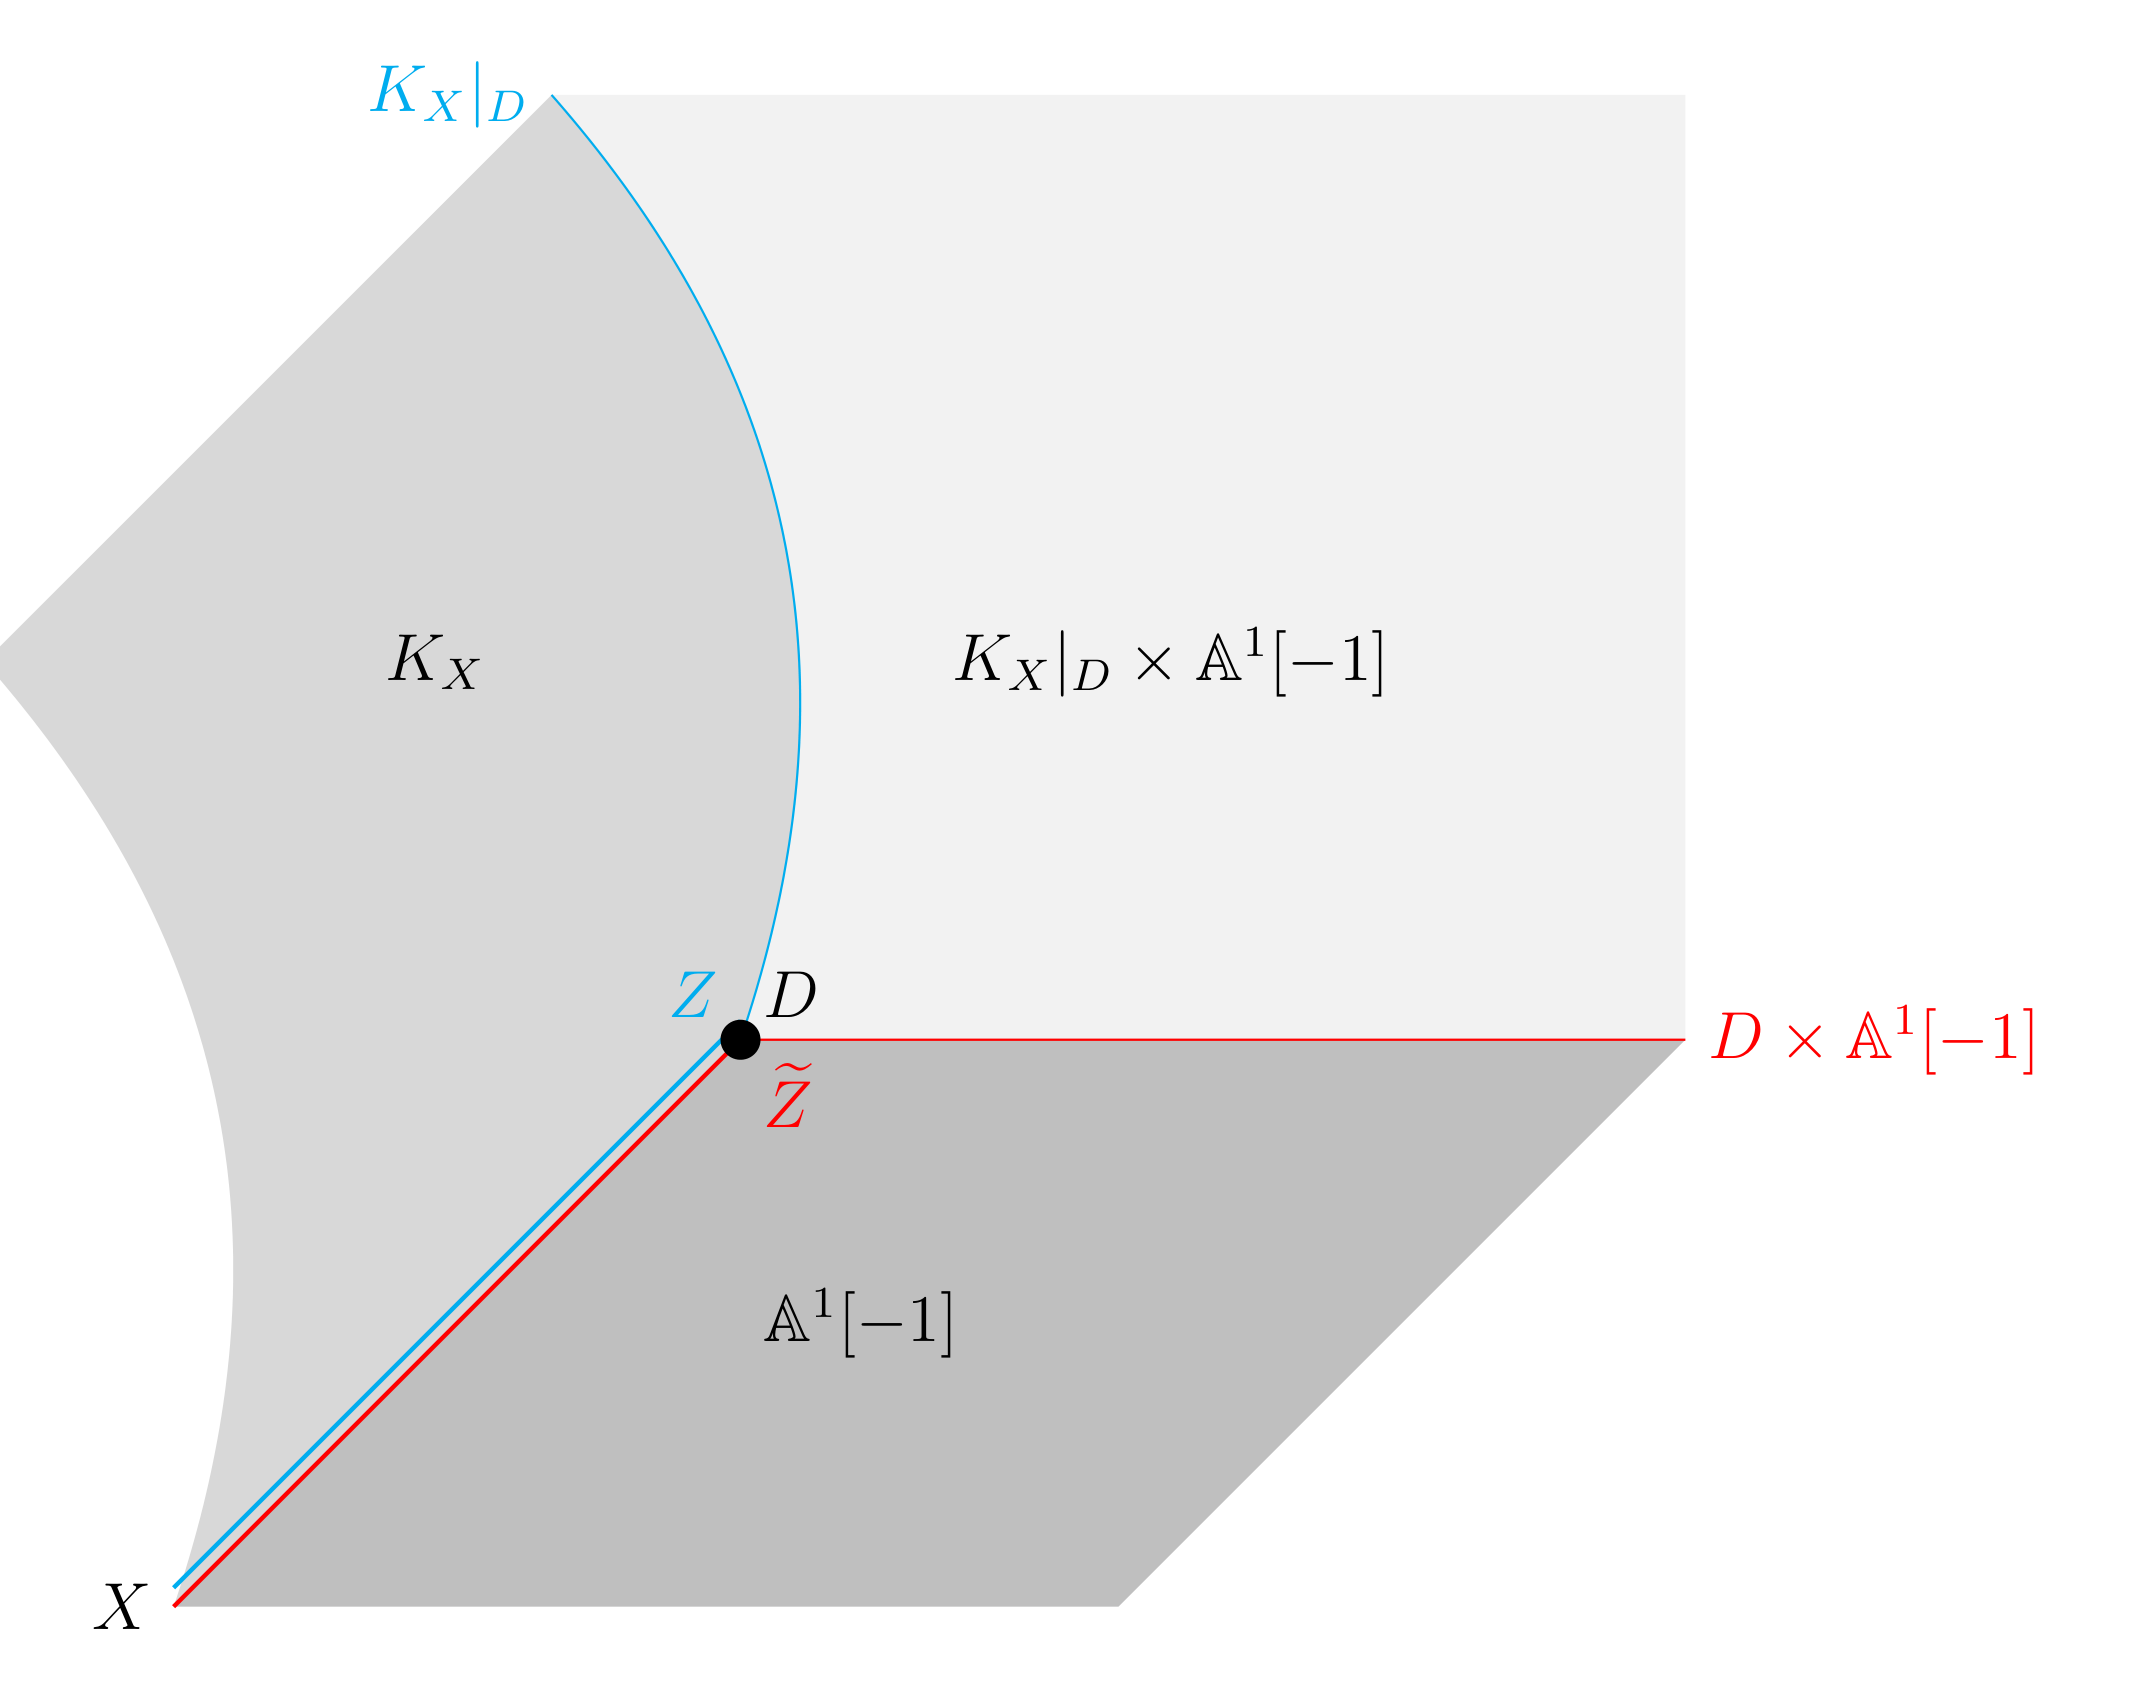
\includegraphics[width=0.66\textwidth]{figures/fig8_1.png}
\caption{$X=\mathbb A^1$ 时 $\cK_X\times\mathbb A^1[-1]$ 的示意图。}
\label{fig:8-1}
\end{figure}

\begin{lemma}\label{lem:8-1-2}
Kn{\"o}rrer 周期性给出 dg 函子的交换图表：
\[
\begin{tikzcd}[column sep=3.4em, row sep=1.9em]
& \operatorname{Coh}_{\mathbb G_m}(\cK_X\times\mathbb A^1,s(x)yz) & \\
\operatorname{Coh}(Z) \arrow[ur] & & \operatorname{Coh}(\tilde Z) \arrow[ul] \\
& \operatorname{Coh}(X) \arrow[ul, "{\pi_X^*[1]}"'] \arrow[ur, "i_{\tilde X*}"'] &
\end{tikzcd}
\]
\end{lemma}

\begin{proof}
设 $\mathcal E=\pi_X^*\mathcal F$ 是 $X$ 上局部自由层（locally free sheaf）$\mathcal F$ 的拉回，并记 $p_Z$ 为投影 $Z\times\mathbb A^1\to Z$。左上等价 $\operatorname{Coh}(Z)\to\operatorname{Coh}_{\mathbb G_m}(\cK_X\times\mathbb C,s(x)yz)$ 把 $\mathcal E$ 送到 $p_Z^*\mathcal E$ 沿包含 $j_Z\colon Z\times\mathbb A^1\to\cK_X\times\mathbb A^1$ 的推前。注意

% ===== 原书 p.115 =====
$\hat Z$ 上存在相干层的正合列
\[
0\to\OO_{Z\times\mathbb A^1}\to\OO_{\hat Z}\to\OO_{\cK_X\times\{0\}}\to0,
\]
它由函数的限制 $\OO_{\hat Z}\to\OO_{\cK_X\times\{0\}}$ 给出（这里没有正规丛（normal bundle）修正，因为 $\cK_X\times\{0\}=\{z=0\}$ 是平凡线丛的一个截面的零点轨迹（zero-locus））。对投影 $p_{\hat Z}\colon\hat Z\to X$，拉回 $p_{\hat Z}^*\mathcal F$ 是局部自由层。把它与上述正合列作张量积，得到正合三角
\[
\begin{tikzcd}[column sep=4.2em, row sep=1.5em]
j_{Z*}p_Z^*\mathcal E \arrow[rr] & & p_{\hat Z}^*\mathcal F \arrow[dl] \\
& \OO_{\cK_X\times\{0\}}\otimes p_{\hat Z}^*\mathcal F \arrow[ul, "+1"'] &
\end{tikzcd}
\]
\transnote{易错预警：正合三角回边上的 $+1$ 表示平移（shift），不是符号；三条边依次为 $j_{Z*}p_Z^*\mathcal E$、$p_{\hat Z}^*\mathcal F$、$\OO_{\cK_X\times\{0\}}\otimes p_{\hat Z}^*\mathcal F$。}
注意：过渡到商范畴 $\operatorname{Sing}(\hat Z)$ 会把所有局部自由层送到零。于是 $j_{Z*}p_Z^*\mathcal E[1]$ 在 $\operatorname{Sing}(\hat Z)$ 中等价于层 $\OO_{\cK_X\times\{0\}}\otimes p_{\hat Z}^*\mathcal F$。而后者恰好是 $i_{\tilde X*}\mathcal E|_X$ 在 $\operatorname{Coh}(\cK_X\times\mathbb C)$ 中的像，取像的函子为 $j_{\tilde Z*}p_{\tilde Z}^*\colon\operatorname{Coh}(\tilde Z)\to\operatorname{Coh}_{\mathbb G_m}(\cK_X\times\mathbb C,s(x)yz)$。由于 $X$ 光滑，该图表对所有相干层也交换。

接下来需要检查图表在态射层面交换。不妨设 $h\colon\mathcal F\to\mathcal G$ 是 $X$ 上局部自由层之间的态射。沿左手边把箭头走一遍，得到矩阵分解的态射
\[
\tilde h\colon\OO_{Z\times\mathbb A^1}\otimes p_{\hat Z}^*\mathcal F[1]\to\OO_{Z\times\mathbb A^1}\otimes p_{\hat Z}^*\mathcal G[1];
\]
而在右手边得到态射
\[
\tilde h\colon\OO_{\cK_X\times\{0\}}\otimes p_{\hat Z}^*\mathcal F\to\OO_{\cK_X\times\{0\}}\otimes p_{\hat Z}^*\mathcal G,
\]
其中 $\tilde h(x,y,z)=h(x)$。在我们选定的同构 $\OO_{\cK_X\times\{0\}}\cong\OO_{Z\times\mathbb A^1}[1]$ 之下，两者互相等同。
\end{proof}

\begin{definition}\label{def:8-1-3}
函子 $q\colon\overline{\operatorname{Coh}}(Z)\to\overline{\operatorname{Sing}}(Z)$ 是 dg 商函子（dg quotient functor），它把所有完美复形（perfect complex）送到零。
\end{definition}

% ===== 原书 p.116 =====
\begin{definition}\label{def:8-1-4}
局部化函子（localization functor）loc 把 $\overline{\operatorname{Coh}}(D\times\C^\times[-1])$ 映射到 $\overline{\operatorname{Coh}}(D)$：它局部化于一个 2 次自然变换，该自然变换由 $\C[z^{\pm1}]\cong\End(\OO_{\C^\times[-1]})$ 的生成元 $z$ 的作用给出（见引理 \ref{lem:koszul-duality}）。
\end{definition}

可与命题 \ref{prop:8-2-2} 对照。注意这两个函子（按这里的呈现方式）都只是 $\Z/2$-分次的。

\transnote{易错预警：本节起大量范畴带上横线（如 $\overline{\operatorname{Coh}}$），它表示同调分次的模 2 约化，不是复共轭或闭包。}

\begin{proposition}\label{prop:8-1-5}
在定理 \ref{thm:6-1-16} 中的 Kn{\"o}rrer 等价之下，我们有 $\C((\beta))$-线性 dg 范畴的交换图表：
\[
\begin{tikzcd}[column sep=3.0em, row sep=1.7em]
\overline{\operatorname{Coh}}(\tilde Z) \arrow[r, "j_{\tilde D}^*"] \arrow[d, "{\sim}"'] & \overline{\operatorname{Coh}}(D\times\C^\times[-1]) \arrow[r, "loc"] & \overline{\operatorname{Coh}}(D) \arrow[dd, "{\sim}"'] \\
\overline{\operatorname{Coh}}_{\mathbb G_m}(\cK_X\times\mathbb A^1,s(x)yz) & & \\
\overline{\operatorname{Coh}}(Z) \arrow[u, "{\sim}"'] \arrow[rr, "q"'] & & \overline{\operatorname{Sing}}(Z)
\end{tikzcd}
\]
\end{proposition}

\begin{proof}
设 $\mathcal E$ 是 $Z$ 上的局部自由层：它可以由某个 $X$ 上的局部自由层拉回得到。于是在引理 \ref{lem:8-1-2} 的等价链 $\operatorname{Coh}(Z)\to\operatorname{Coh}(\tilde Z)$ 之下，$\mathcal E$ 被送到 $i_{\tilde X*}\mathcal E|_X[-1]$，而后者在拉回到 $D\times\C^\times$ 的映射下显然被送到零。因此沿图表两个方向走，都把 $Z$ 上所有局部自由层送到零。

% ===== 原书 p.117 =====
第二部分的论证如下。由引理 \ref{lem:6-1-7}，$\C((\beta))$-线性等价 $\overline{\operatorname{Coh}}(D)\to\overline{\operatorname{Sing}}(Z)$ 通过商映射 $q$ 分解；因此 $q$ 在那些经由 $j_{D*}p_D^*$ 来自 $D$ 的层上是等价（这里 $p_D\colon\cK_X|_D\to D$、$j_D\colon\cK_X|_D\to Z$ 分别为投影与包含）。于是设 $\mathcal F$ 是 $Z$ 上支撑在 $\cK_X|_D$ 上的相干层，且经由 $\mathcal F=j_{D*}p_D^*\mathcal F_D$ 来自 $D$。由引理 \ref{lem:8-1-1}，这个层被送到 $\operatorname{Coh}(\tilde Z)$ 中的层 $\tilde{\mathcal F}$，其中 $\tilde{\mathcal F}=j_{\tilde D*}p_{\tilde D}^*\mathcal F_D$。注意：顶行的复合 $\operatorname{Coh}(\tilde Z)\to\operatorname{Coh}(D)$ 把 $\tilde{\mathcal F}$ 送到 $\mathcal F_D$。在引理 \ref{lem:6-1-7} 的等价之下，$\mathcal F_D$ 被送到矩阵分解 $F$：
\[
F_0=\bigoplus_{n\in\Z}i_{Z*}j_{D*}p_D^*\cF_D^{2n}(\chi^{-n}),\qquad
F_1=\bigoplus_{m\in\Z}i_{Z*}j_{D*}p_D^*\cF_D^{2m+1}(\chi^{-m}),
\]
它位于 $\operatorname{Coh}_{\mathbb G_m}(\cK_X,s(x)y)$ 中。另一方面，$\mathcal F$ 在 $\operatorname{Coh}(Z)$ 中被送到层 $i_{Z*}\mathcal F$，后者同样给出 $\operatorname{Coh}_{\mathbb G_m}(\cK_X,s(x)y)$ 中的一个矩阵分解。作为 $\Z/2$-分次的矩阵分解，这与上面的 $F$ 相同，因为 $\mathcal F=j_{D*}p_D^*\mathcal F_D$。

类似地，设 $h_D\colon\mathcal F_D\to\mathcal G_D$ 是 $D$ 上相干层复形的 $k$ 次态射；由引理 \ref{lem:6-1-7}，$\tilde Z$ 上对应的相干层态射 $\tilde h\colon\tilde{\mathcal F}\to\tilde{\mathcal G}$ 也以 $j_{\tilde D*}p_{\tilde D}^*(h_D)$ 的形式出现，次数同为 $k$。由于 $\tilde h$ 与 $z$ 无关，在局部化函子之下 $\tilde h$ 直接被送到 $\Hom^{k\,(\mathrm{mod}\,2)}(\mathcal F_D,\mathcal G_D)$ 中的 $h_D$。这说明：当态射的次数模 2 计时，图表交换。
\end{proof}

\subsection{镜像对称}

% ===== 原书 p.118 =====
首先，我们可以给出猜想 \ref{conj:aur-funct} 第 3 部分的一个版本：

\begin{theorem}\label{thm:8-2-1}
$\cW_0((\C^*)^n\setminus H)$ 与 $\operatorname{Coh}(Z)$ 之间存在镜像对称等价：它由定理 \ref{thm:7-2-4} 中 $\cW_0((\C^*)^n\setminus H)$ 与 $\operatorname{Coh}(\tilde Z)$ 的镜像等价，复合定理 \ref{thm:6-1-16} 中的等价链 $\operatorname{Coh}(\tilde Z)\to\operatorname{Coh}(Z)$ 得到。

在此等价之下，函子 $\alpha_\infty\colon\cW((\C^*)^n,f)\to\cW_0((\C^*)^n\setminus H)$ 镜像于 $\pi_X^*[1]\colon\operatorname{Coh}(X)\to\operatorname{Coh}(Z)$。
\end{theorem}

\transnote{易错预警：定理 \ref{thm:8-2-1} 的等价不是一步给出的，而是「定理 \ref{thm:7-2-4} 的等价」与「定理 \ref{thm:6-1-16} 的等价链」的复合；函子 $\alpha_\infty$ 的像 $\pi_X^*[1]$ 也须在这一复合下理解。}

\begin{proof}
应用引理 \ref{lem:8-1-2} 即得。
\end{proof}

来自 [Aur18, §4] 的限制函子 $\rho\colon\cW_0((\C^*)^n\setminus H)\to\cW(H)$ 在某种意义上是唯一的，因此我们在这里花些篇幅描述它。这样的函子甚至是否存在，远非显而易见：分次的选择尤其重要。

限制函子定义的第一步由 Viterbo 限制 [GPS19, §11.1] 给出：从 $(\C^*)^n\setminus H$ 限制到命题 \ref{prop:7-1-1} 第 (1) 部分的子区域 $H\times\C^*$。这一步可以在 $\Z$-分次范畴的层面上完成。此外，由于 $H\times\C^*$ 是 Weinstein 流形，Viterbo 限制函子可以定义在扭复形范畴上 [GPS19, (11.5)]。

由 [GPS19, Corollary 1.18] 的 K{\"u}nneth 定理，wrapped Fukaya 范畴 $\cW(H\times\C^*(2))$ 由形如 $\ell\times\R_{>0}$ 的对象的（柱化，cylindrization）生成，其中 $\ell$ 是 $H$ 中的拉格朗日量。在对象层面，函子 $\rho$ 应当把 $\ell\times\R_{>0}$ 送到 $\ell$：然而它在态射层面是否良定义并不清楚，因为没有可选取的参考纤维 $H\times\{p\}$，用来在 $H\times\C^*$ 中取两个拉格朗日量的相交。可是，如果我们使用 $H\times\C^*$ 上的 0-分次，它就会良定义：这镜像于代数几何中取 $\mathbb A^1[-1]$ 里「一般点」（generic point）上纤维的构造。

\transnote{背景直觉：没有参考纤维 $H\times\{p\}$，就无法在态射层面取两个拉格朗日量的相交；0-分次相当于用 $\mathbb A^1[-1]$ 上「一般点」的纤维代替这个缺失的参考纤维。}

为说明这一点，我们从最简单的例子开始，其中 $H$ 只是一个点：

% ===== 原书 p.119 =====
\begin{proposition}\label{prop:8-2-2}
当 $|z|=2$ 时，存在从有限生成 $\C[z^{\pm1}]$-模范畴到 $\Z/2$-分次有限维 $\C$ 向量空间范畴的自然函子，它把 $\C[z^{\pm}]$ 送到 0 次的 $\C$。此外，这给出从 $\C[z^{\pm1}]$-模的带分次 dg 范畴（模上带有额外的 $\Z$-分次，且 $z$ 的次数为 0）到 $\C$ 向量空间的分次 $\C((\beta))$-周期 dg 范畴的分次函子。
\end{proposition}

\transnote{易错预警：「$|z|=2$」指 $z$ 作为 2 次映射把分次提高 2，不是 $z$ 的模长；正因如此才能按奇偶取 $F^{2k}$ 与 $F^{2k+1}$。}

\begin{proof}
给定有限生成 $\C[z^{\pm1}]$-模 $F$，它对应于一个有限维 $\C$ 向量空间序列 $F^\bullet$，连同 2 次映射 $z\colon F^k\to F^{k+2}$。于是可以如下定义 $\rho(F)$：对任意 $k\in\Z$，令 $V_0=F^{2k}$、$V_1=F^{2k+1}$。重要的是：给定 $\C[z^{\pm1}]$-模的态射 $f\colon F\to G$，即与 $z$ 交换的线性映射 $f^\bullet\colon F^\bullet\to G^\bullet$，我们通过 $f^0=f^{2k}\colon F^{2k}\to G^{2k}$ 与 $f^1=f^{2k+1}\colon F^{2k+1}\to G^{2k+1}$ 得到态射 $\rho(F)\to\rho(G)$。重要的是：这个定义与 $k\in\Z$ 的选取无关，并给出从有限生成 $\C[z^{\pm1}]$-模到 $\Z/2$-分次 $\C$ 向量空间的函子。
\end{proof}

注意：若改取 $z$ 的次数为 0，则不存在这样的构造：给定以次数 0 的变量 $z$ 写成的 Laurent 多项式，只挑出其中一个系数并不能定义函子。

在一般情形下，$\cW(H\times\C^*(2))$ 中两个对象 $L_1,L_2$ 之间的态射总带有 $\C[z^{\pm1}]$-作用：若 $L_1=\ell_1\times\R_{>0}$、$L_2=\ell_2\times\R_{>0}$，则态射由
\[
\Hom(L_1,L_2)\cong\Hom_{\cW(H)}(\ell_1,\ell_2)\otimes_\C\C[z^{\pm1}]
\]
给出，它带有显然的 $\C[z^{\pm1}]$-作用。给定 $L_1$ 与 $L_2$ 之间的态射 $p$，我们有映射
\[
\Hom^{2k}_{\cW(H\times\C^*(2))}(L_1,L_2)\xrightarrow{\ \sim\ }\Hom^{0}_{\cW(H\times\C^*(2))}(L_1,L_2)\to\Hom^{\mathrm{even}}_{\cW(H)}(\ell_1,\ell_2),
\]
它把 $p$ 的 $2k$ 次部分送到 $z^{-k}p$。类似地，把

% ===== 原书 p.120 =====
$p$ 的 $2k+1$ 次部分送到 $z^{-k}p$，就得到映射
\[
\Hom^{2k+1}_{\cW(H\times\C^*(2))}(L_1,L_2)\xrightarrow{\ \sim\ }\Hom^{1}_{\cW(H\times\C^*(2))}(L_1,L_2)\to\Hom^{\mathrm{odd}}_{\cW(H)}(\ell_1,\ell_2),
\]
对任意 $k\in\Z$ 成立；容易验证它给出从 $\cW(H\times\C^*(2))$ 到 $\Z/2$-分次范畴 $\overline{\cW}(H)$ 的良定义函子。

更精确地说，按照 [Aur18]，我们可以在 $A_\infty$-模上形式地定义 $\rho$：沿包含函子 $i\colon\cW(H)\to\cW(H\times\C^*(2))$ 拉回，该包含把拉格朗日量 $\ell$ 送到 $\ell\times\R_{>0}$。注意这个构造用到了 $H$ 在 $(\C^*)^n$ 中的一个标架（framing）选取。给定 $\cW(H\times\C^*(2))$ 中的 $L$，拉回模 $i^*(L)$ 绝不能由 $\cW(H)$ 的某个对象表示，因为它的上同调支撑（cohomological support）无界。Auroux 的关键观察是：$\C[z^{\pm1}]$ 的作用给 $i^*(L)$ 诱导出一个 2-周期结构 [Aur18, p.17]，于是 $i^*(L)$ 可由 $\C((\beta))$-线性范畴 $\overline{\cW}(H)$ 中的对象表示，这里我们把分次模 2 约化。某种意义上，范畴 $\cW(H\times\C^*(2))$ 只是 $\cW(H)$ 的 2-周期化（2-periodization）。函子 $\rho$ 恰好对应于局部化 $\cW(H\times\C^*(2))\to\overline{\cW}(H)$，局部化于 2 次自然变换 $z\colon\id\to[2]$，该变换由绕 $0$ 旋转 $\C^*$ 给出 [Aur18, (4.3)]，从而得到 $\Z/2$-分次范畴。总结如下：

\begin{definition}\label{def:8-2-3}
限制函子 $\rho\colon\overline{\cW}_0((\C^*)^n\setminus H)\to\overline{\cW}(H)$ 的定义如下：先取到命题 \ref{prop:7-1-1} 第 (1) 部分中区域 $H\times\C^*$ 的 Viterbo 限制；再取局部化函子 $\overline{\cW}(H\times\C^*(2))\to\overline{\cW}(H)$，局部化于由 $\End_{\cW(\C^*(2))}(\R_{>0})\cong\C[z^{\pm1}]$ 的生成元 $z$ 的乘法给出的 2 次自然变换（见 [Aur18, (4.3)]）。
\end{definition}

\transnote{含糊点拨：局部化于 2 次自然变换会把同调分次 2-周期化，因此只剩下 $\Z/2$-分次；这正是 $\rho$ 不能写成 $\Z$-分次函子的原因。}

回忆我们用上横线表示 $A_\infty$ 范畴同调分次的模 2 约化：$\overline{\cW}_0((\C^*)^n\setminus H)$

% ===== 原书 p.121 =====
与 $\overline{\operatorname{Coh}}(Z)$。注意这个 $\rho$ 函子只是 $\C((\beta))$-线性 $A_\infty$ 范畴的函子，因为我们局部化于一个 2 次自然变换。

\begin{proposition}\label{prop:8-2-4}
在上述关于函数 $\tilde f_0$ 的镜像对称等价之下，从 $(\C^*)^n\setminus H$ 到 $H\times\C^*$ 的 Viterbo 限制镜像于从 $\tilde Z$ 到 $D\times\C^*[-1]$ 的拉回：也就是说，$A_\infty$ 范畴的如下图表交换：
\[
\begin{tikzcd}[column sep=3.6em, row sep=1.7em]
\cW_0((\C^*)^n\setminus H) \arrow[r] \arrow[d, "\mathrm{Vit}"'] & \operatorname{Coh}(\tilde Z) \arrow[d, "j_{\tilde D}^*"] \\
\cW(H\times\C^*(2)) \arrow[r] & \operatorname{Coh}(D\times\C^*[-1])
\end{tikzcd}
\]
\end{proposition}

\begin{proof}
这由 [GS21, Corollary 5.8] 推出。
\end{proof}

\transnote{易错预警：命题 \ref{prop:8-2-4} 的图表照原书不带横线，与定理 \ref{thm:8-2-5} 的带横线版本不同；这是原书的不一致，译文照录。}

\begin{theorem}\label{thm:8-2-5}
限制函子 $\rho\colon\overline{\cW}_0((\C^*)^n\setminus H)\to\overline{\cW}(H)$ 镜像于商函子 $q\colon\overline{\operatorname{Coh}}(Z)\to\overline{\operatorname{Sing}}(Z)$ 与 Kn{\"o}rrer 周期性等价 $\overline{\operatorname{Sing}}(Z)\to\overline{\operatorname{Coh}}(D)$ 的复合（作为 $\C((\beta))$-线性 $A_\infty$ 范畴的函子，见引理 \ref{lem:6-1-7}）；这里的镜像对应在定理 \ref{thm:8-2-1} 的镜像对称等价之下。
\end{theorem}

\begin{proof}
在下面的图表中，左上方的方块由命题 \ref{prop:8-2-4} 交换；右上方的方块显然也交换，因为我们局部化于同一个自然变换。剩下要证下方方块交换，这正是命题 \ref{prop:8-1-5}。
\end{proof}

% ===== 原书 p.122 =====
\[
\begin{tikzcd}[column sep=3.0em, row sep=1.7em]
\overline{\cW}_0((\C^*)^n\setminus H) \arrow[r, "\mathrm{Vit}"] \arrow[rr, bend left=24, "\rho"] \arrow[d, "{\sim}"'] & \overline{\cW}(H\times\C^*(2)) \arrow[r, "loc"] \arrow[d, "{\sim}"'] & \overline{\cW}(H) \arrow[d, "{\sim}"'] \\
\overline{\operatorname{Coh}}(\tilde Z) \arrow[r, "j_{\tilde D}^*"] \arrow[d, "{\sim}"'] & \overline{\operatorname{Coh}}(D\times\C^\times[-1]) \arrow[r, "loc"] & \overline{\operatorname{Coh}}(D) \arrow[dd, "{\sim}"'] \\
\overline{\operatorname{Coh}}_{\mathbb G_m}(\cK_X\times\mathbb A^1,s(x)yz) & & \\
\overline{\operatorname{Coh}}(Z) \arrow[u, "{\sim}"'] \arrow[rr, "q"'] & & \overline{\operatorname{Sing}}(Z)
\end{tikzcd}
\]

\subsection{整分次增强}

到目前为止我们看到：函子 $q$ 与 $\rho$ 在一个 $\Z/2$-分次的同调镜像对称等价之下对应，即在一个 $\C((\beta))$-线性范畴的等价之下对应。本节要说明：所涉及的范畴都带有一个辅助的 $\Z$-分次，并且 $q$ 与 $\rho$ 可以在分次 $\C((\beta))$-线性范畴的等价之下对应起来。

\begin{definition}\label{def:8-3-1}
我们引入如下术语：
\begin{itemize}
\item 我们把由「在 $\mathbb G_m$-作用下给 $\mathbb A^1$ 权（weight）1」而来的分次，连同 $(\C^*)^n\setminus H$ 上的形式 $\eta_0$，称为\textbf{0-分次（0-grading）}；我们把它看作范畴上底层的同调分次结构。
\item 我们把由「在 $\mathbb G_m$-作用下给 $\cK_X$ 的纤维权 1」而来的分次，连同 $(\C^*)^n\setminus H$ 上的形式 $\eta_\infty$，称为\textbf{$\infty$-分次（$\infty$-grading）}；我们把它看作范畴上的
\end{itemize}
\end{definition}

% ===== 原书 p.123 =====
额外 $\Z$-分次结构。

使用 $\infty$-分次，就在 $A_\infty$ 范畴 $\cW_{0,\infty}((\C^*)^n\setminus H)$ 与 $\operatorname{Coh}_{\mathbb G_m}(Z)$ 上得到（额外的）分次；把同调分次模 2 约化，便得到分次 $\C((\beta))$-线性 $A_\infty$ 范畴。我们仍用上横线表示同调分次的模 2 约化（reduction mod 2）：$\overline{\cW}_{0,\infty}((\C^*)^n\setminus H)$ 与 $\overline{\operatorname{Coh}}_{\mathbb G_m}(Z)$。

现在可以定义限制函子 $\rho\colon\overline{\cW}_{0,\infty}((\C^*)^n\setminus H)\to\overline{\cW}(H)$ 的分次版本，步骤如下：
\begin{itemize}
\item 先取到子区域 $H\times\C^*$ 的 Viterbo 限制（[GPS19] 中的定义可以按分次方式执行），其中 $H\times\C^*$ 带有从 $(\C^*)^n\setminus H$ 的行列式丛（determinant bundle）平凡化限制而来的平凡化；然后，
\item 取局部化 $\overline{\cW}_{0,\infty}(H\times\C^*)\to\overline{\cW}(H)$，局部化于乘以 2 次自然变换 $z$。由于在 $\infty$-分次下乘以 $z$ 的次数为 0，后一个函子由命题 \ref{prop:8-2-2} 是分次 $A_\infty$ 函子。
\end{itemize}
于是 $\rho$ 是分次 $\C((\beta))$-线性 $A_\infty$ 范畴之间的分次函子（graded functor）。

同样地，等变相干层（equivariant coherent sheaf）上的商映射 $q\colon\operatorname{Coh}_{\mathbb G_m}(Z)\to\operatorname{Sing}_{\mathbb G_m}(Z)$ 不保持同调分次，但保持由 $\mathbb G_m$-等变结构给出的分次（参引理 \ref{lem:6-1-7}），后者正是 $\infty$-分次。于是它给出分次 $\C((\beta))$-线性 dg 范畴的分次函子 $q\colon\overline{\operatorname{Coh}}_{\mathbb G_m}(Z)\to\overline{\operatorname{Sing}}_{\mathbb G_m}(Z)$（这里 $\operatorname{Sing}_{\mathbb G_m}(Z)$ 上的 $\C((\beta))$-线性结构来自定理 \ref{thm:zgraded-orlov} 中与矩阵分解范畴的等价）。

这样，$\rho$ 与 $q$ 都有提升为分次函子的版本。接下来我们要说明，它们在分次意义下于镜像对称之下对应。

% ===== 原书 p.124 =====
\begin{lemma}\label{lem:8-3-2}
分次 $A_\infty$ 范畴 $\cW_{0,\infty}((\C^*)^n,f)$ 与 $\operatorname{Coh}_{\mathbb G_m^2}(X,0)$ 之间存在镜像对称等价，连同交换图表
\[
\begin{tikzcd}[column sep=3.6em, row sep=1.7em]
\cW(H) \arrow[r] \arrow[d, "\cup"'] & \operatorname{Coh}(D) \arrow[d, "i_{D*}"] \\
\cW_{0,\infty}((\C^*)^n,f) \arrow[r] & \operatorname{Coh}_{\mathbb G_m^2}(X,0)
\end{tikzcd}
\]
其中竖直箭头是 [GS22] 的等价。
\end{lemma}

\transnote{易错预警：$\mathbb G_m^2$ 指两个 $\mathbb G_m$-作用的积，不是群 $\mathbb G_m$ 的平方；两个作用分别来自 $X$ 与 $\mathbb A^1$。}

\begin{proof}
这不过是一个观察：行列式丛在任意一般纤维 $H$ 上与在 $((\C^*)^n,f)$ 上的两个平凡化在相差同伦的意义下一致；再结合两个 $\mathbb G_m$-作用在 $X$ 上都平凡这一事实。前者可以从命题 \ref{prop:7-1-1} 与 \ref{prop:7-1-2} 的每个粘合呈现都不改变子扇形 $((\C^*)^n,f)$ 看出。
\end{proof}

\transnote{含糊点拨：原书此处作 “The former is can be seen”，系笔误；译文按「前者可以从……看出」处理。}

\begin{theorem}\label{thm:8-3-3}
分次 $A_\infty$ 范畴 $\cW_{0,\infty}((\C^*)^n\setminus H)$ 与 $\operatorname{Coh}_{\mathbb G_m^2}(\tilde S,0)$ 之间存在镜像对称等价。
\end{theorem}

\begin{proof}
检查 [GPS19] 的论证可以发现：命题 \ref{prop:7-1-1} 的扇形分解给出分次 $A_\infty$ 范畴的推出图表（参 [GPS19, p.26]）：
\[
\begin{tikzcd}[column sep=4.0em, row sep=1.7em]
\cW(H) \arrow[r, "\cup"] \arrow[d] & \cW_{0,\infty}((\C^*)^n,f) \arrow[d] \\
\cW_{0,\infty}(H\times\C^*,z) \arrow[r] & \cW_{0,\infty}((\C^*)^n\setminus H)
\end{tikzcd}
\]
\transnote{易错预警：定理 \ref{thm:8-3-3} 的推出图表中两个竖直箭头没有标函子名（与推论 \ref{cor:7-1-4} 同），它们是扇形包含给出的函子，并非漏标。}
\end{proof}

% ===== 原书 p.125 =====
我们把这一粘合图表与命题 \ref{prop:6-2-2} 的粘合图表作比较：
\[
\begin{tikzcd}[column sep=3.0em, row sep=1.7em]
& \operatorname{Coh}_{\mathbb G_m^2}(D,0) \arrow[rr, "\iota_{\tilde D*}"] \arrow[dd, "i_{D*}"', pos=0.1] & & \operatorname{Coh}_{\mathbb G_m^2}(D\times\mathbb A^1,0) \arrow[dd, "j_{\tilde D*}", pos=0.1] \\
\cW(H) \arrow[ur, "{\sim}"] \arrow[rr, "\cup", pos=0.3] \arrow[dd, "\cup"'] & & \cW_{0,\infty}(H\times\C^*,z) \arrow[ur, "{\sim}"] \arrow[dd] & \\
& \operatorname{Coh}_{\mathbb G_m^2}(X,0) \arrow[rr, "i_{\tilde X*}"'] & & \operatorname{Coh}_{\mathbb G_m^2}(\tilde S,0) \\
\cW_{0,\infty}((\C^*)^n,f) \arrow[ur, "{\sim}"] \arrow[rr, "\alpha_\infty"'] & & \cW_{0,\infty}((\C^*)^n\setminus H) \arrow[ur, "{\sim}"] &
\end{tikzcd}
\]
\transnote{含糊点拨：此图中左竖与横中两条箭头都标 $\cup$，但它们是两个不同的 cup 函子：一条 $\cW(H)\to\cW_{0,\infty}((\C^*)^n,f)$，另一条 $\cW(H)\to\cW_{0,\infty}(H\times\C^*,z)$。}
再借助引理 \ref{lem:8-3-2} 便得到所需的等价。

\begin{proposition}\label{prop:8-3-4}
我们有分次 $A_\infty$ 范畴的交换图表：
\[
\begin{tikzcd}[column sep=3.6em, row sep=1.7em]
\cW_{0,\infty}((\C^*)^n\setminus H) \arrow[r] \arrow[d, "\mathrm{Vit}"'] & \operatorname{Coh}_{\mathbb G_m}(\tilde Z) \arrow[d, "j_{\tilde D}^*"] \\
\cW_{0,\infty}(H\times\C^*) \arrow[r] & \operatorname{Coh}_{\mathbb G_m}(D\times\C^*[-1])
\end{tikzcd}
\]
\end{proposition}

\begin{proof}
检查 [GS21, Corollary 5.8] 与 [FLTZ12] 的论证可以发现，相应结果可以推广到分次 $A_\infty$ 范畴。
\end{proof}

分次 $A_\infty$ 范畴层面的同调镜像对称等价，特别地通过把分次模 2 忘掉，下降到分次 $\C((\beta))$-线性 $A_\infty$ 范畴的层面。

\transnote{背景直觉：整分次增强的意思是——先把分次结构本身做成数据（0-分次或 $\infty$-分次），再要求 $q$ 与 $\rho$ 在这个分次意义下对应；单纯的 $\Z/2$ 等价无法区分两种分次。}

\begin{proposition}\label{prop:8-3-5}
在定理 \ref{thm:6-2-1} 中的 Kn{\"o}rrer 等价之下，我们有分次 $\C((\beta))$-线性 dg 范畴的交换图表：
\[
\begin{tikzcd}[column sep=2.6em, row sep=1.6em]
\overline{\operatorname{Coh}}_{\mathbb G_m^2}(\tilde S,0) \arrow[r, "j_{\tilde D}^*"] \arrow[d, "{\sim}"'] & \overline{\operatorname{Coh}}_{\mathbb G_m^2}(D\times\C^\times,0) \arrow[r, "loc"] & \overline{\operatorname{Coh}}(D) \arrow[dd, "{\sim}"'] \\
\overline{\operatorname{Coh}}_{\mathbb G_m^2}(\cK_X\times\mathbb A^1,s(x)yz) & & \\
\overline{\operatorname{Coh}}_{\mathbb G_m^2}(Z,0) \arrow[u, "{\sim}"'] \arrow[rr, "q"'] & & \overline{\operatorname{Sing}}_{\mathbb G_m}(Z)
\end{tikzcd}
\]
其中 $\operatorname{Coh}_{\mathbb G_m^2}(Z,0)$ 按引理 \ref{lem:6-2-3} 与 $\operatorname{Coh}_{\mathbb G_m}(Z)$ 等同。
\end{proposition}

% ===== 原书 p.126 =====
\begin{proof}
我们检查命题 \ref{prop:8-1-5} 的证明。第一，容易看出引理 \ref{lem:8-1-1} 与 \ref{lem:8-1-2} 也推广到分次 dg 版本。于是和前面一样，沿图表两个方向走，都把 $Z$ 上所有局部自由等变相干层送到零。重要的是：引理 \ref{lem:6-1-7} 中经由 $\operatorname{Coh}_{\mathbb G_m}(Z)$ 分解的等价是分次 dg 函子。现在，左侧的竖直等价由定理 \ref{thm:6-2-1} 是分次 dg 等价；而顶部的箭头只是分次 $\C((\beta))$-线性 dg 函子，因为局部化把同调分次 2-周期化了。把这些观察与命题 \ref{prop:8-1-5} 的证明结合起来，即得结论。
\end{proof}

\begin{theorem}\label{thm:8-3-6}
限制函子 $\rho\colon\overline{\cW}_{0,\infty}((\C^*)^n\setminus H)\to\overline{\cW}(H)$ 镜像于商函子 $q\colon\overline{\operatorname{Coh}}_{\mathbb G_m}(Z)\to\overline{\operatorname{Sing}}_{\mathbb G_m}(Z)$ 与引理 \ref{lem:6-1-7} 中 Kn{\"o}rrer 周期性等价 $\operatorname{Sing}_{\mathbb G_m}(Z)\to\operatorname{Coh}(D)$ 的复合（作为分次 $\C((\beta))$-线性 $A_\infty$ 函子）；这里的镜像对应在定理 \ref{thm:8-3-3} 的镜像对称等价复合定理 \ref{thm:6-2-1} 的 Orlov 等价之下。
\end{theorem}

\begin{proof}
和前面一样，这由命题 \ref{prop:8-3-4} 与 \ref{prop:8-3-5} 组合即得。
\end{proof}

% ===== 原书 p.127 =====
\[
\begin{tikzcd}[column sep=2.8em, row sep=1.6em]
\overline{\cW}_{0,\infty}((\C^*)^n\setminus H) \arrow[r, "\mathrm{Vit}"] \arrow[rr, bend left=24, "\rho"] \arrow[d, "{\sim}"'] & \overline{\cW}_{0,\infty}(H\times\C^*) \arrow[r, "loc"] \arrow[d, "{\sim}"'] & \overline{\cW}(H) \arrow[d, "{\sim}"'] \\
\overline{\operatorname{Coh}}_{\mathbb G_m^2}(\tilde S,0) \arrow[r, "j_{\tilde D}^*"] \arrow[d, "{\sim}"'] & \overline{\operatorname{Coh}}_{\mathbb G_m^2}(D\times\C^\times,0) \arrow[r, "loc"] & \overline{\operatorname{Coh}}(D) \arrow[dd, "{\sim}"'] \\
\overline{\operatorname{Coh}}_{\mathbb G_m^2}(\cK_X\times\mathbb A^1,s(x)yz) & & \\
\overline{\operatorname{Coh}}_{\mathbb G_m^2}(Z,0) \arrow[u, "{\sim}"'] \arrow[rr, "q"'] & & \overline{\operatorname{Sing}}_{\mathbb G_m}(Z)
\end{tikzcd}
\]

\clearpage
% EN49 c12 | 原书 p.128–134（PDF 139–145）| 第 9 章：提升函子（§9.1 一个例子）
% 每页起首以 % ===== 原书 p.N ===== 注释标记。

\section{提升函子}

% ===== 原书 p.128 =====

超曲面 $H$ 带有由函数 $f$ 给出的自然标架。我们首先要验证：这一标架与 [Syl19b, Proposition 2.6]
中由乘积邻域 $H\times\{\operatorname{Re}(z)\ge-\rho\}\subseteq(\C^*)^n$ 给出的标架一致。
注意，在纤维的未扰动部分之上（按 Sylvan 的记号即 $f^{-1}(1/2)$），由 Sylvan 的方案唯一确定的
向量场是 $X=(g\partial_r,0)$ 与 $Y=(0,R_\lambda)$。这里 $R_\lambda$ 是 $\partial X$ 的 Reeb
向量场，光滑函数 $g\colon\partial X\to\R$ 的选取使得 $\omega_X(g\partial_r,R_\lambda)=1$。
这两个向量场分别是 $\nabla|f|$ 与 $\nabla\arg(f)$ 的正倍数，因此与由 $f$ 在纤维内部区域上
得到的标架一致。完整纤维 $\hat F$ 是把一个无限柱面粘到 $\partial F$ 上得到的（见 [Syl19b,
Proposition 2.6, condition (3)]）。所以，把这一标架延拓到整个纤维，所得结果与 Sylvan 的
构造同伦。

\transnote{易错预警：原文的两个向量场写作 $X=(g\partial_r,0)$、$Y=(0,R_\lambda)$，它们是乘积
$H\times\C^*$ 上的向量场；$R_\lambda$ 属于 $\partial X$ 的 Reeb 方向，$g\partial_r$ 属于另一个
因子。阅读时不要把 $X,Y$ 误当成 $H$ 上或 $\partial X$ 上的向量场。}

\begin{definition}\label{def:9-0-1}
我们定义提升函子（lifting functor）
\[
j\colon\cW(H)\longrightarrow\cW(H\times\C^*,z)\longrightarrow\cW((\C^*)^n\setminus H).
\]
其构造如下：按命题 \ref{prop:7-1-1} 取一个扇形分解，先与 $\R_{\ge0}$ 作乘积并柱化（cylindrization），
再作扇形包含（见图 \ref{fig:9-1}）。
\end{definition}

\transnote{背景直觉：提升函子是一条两步复合。第一步把 $H$ 上的拉格朗日对象沿新增的
$\C^*$ 方向“抬起”，第二步借扇形包含把它搬进 $(\C^*)^n\setminus H$。命题 \ref{prop:7-1-1}
的扇形分解正是为了让这两步都在 Liouville 扇形内完成。}

% ===== 原书 p.129 =====

\begin{figure}[htbp]
\centering
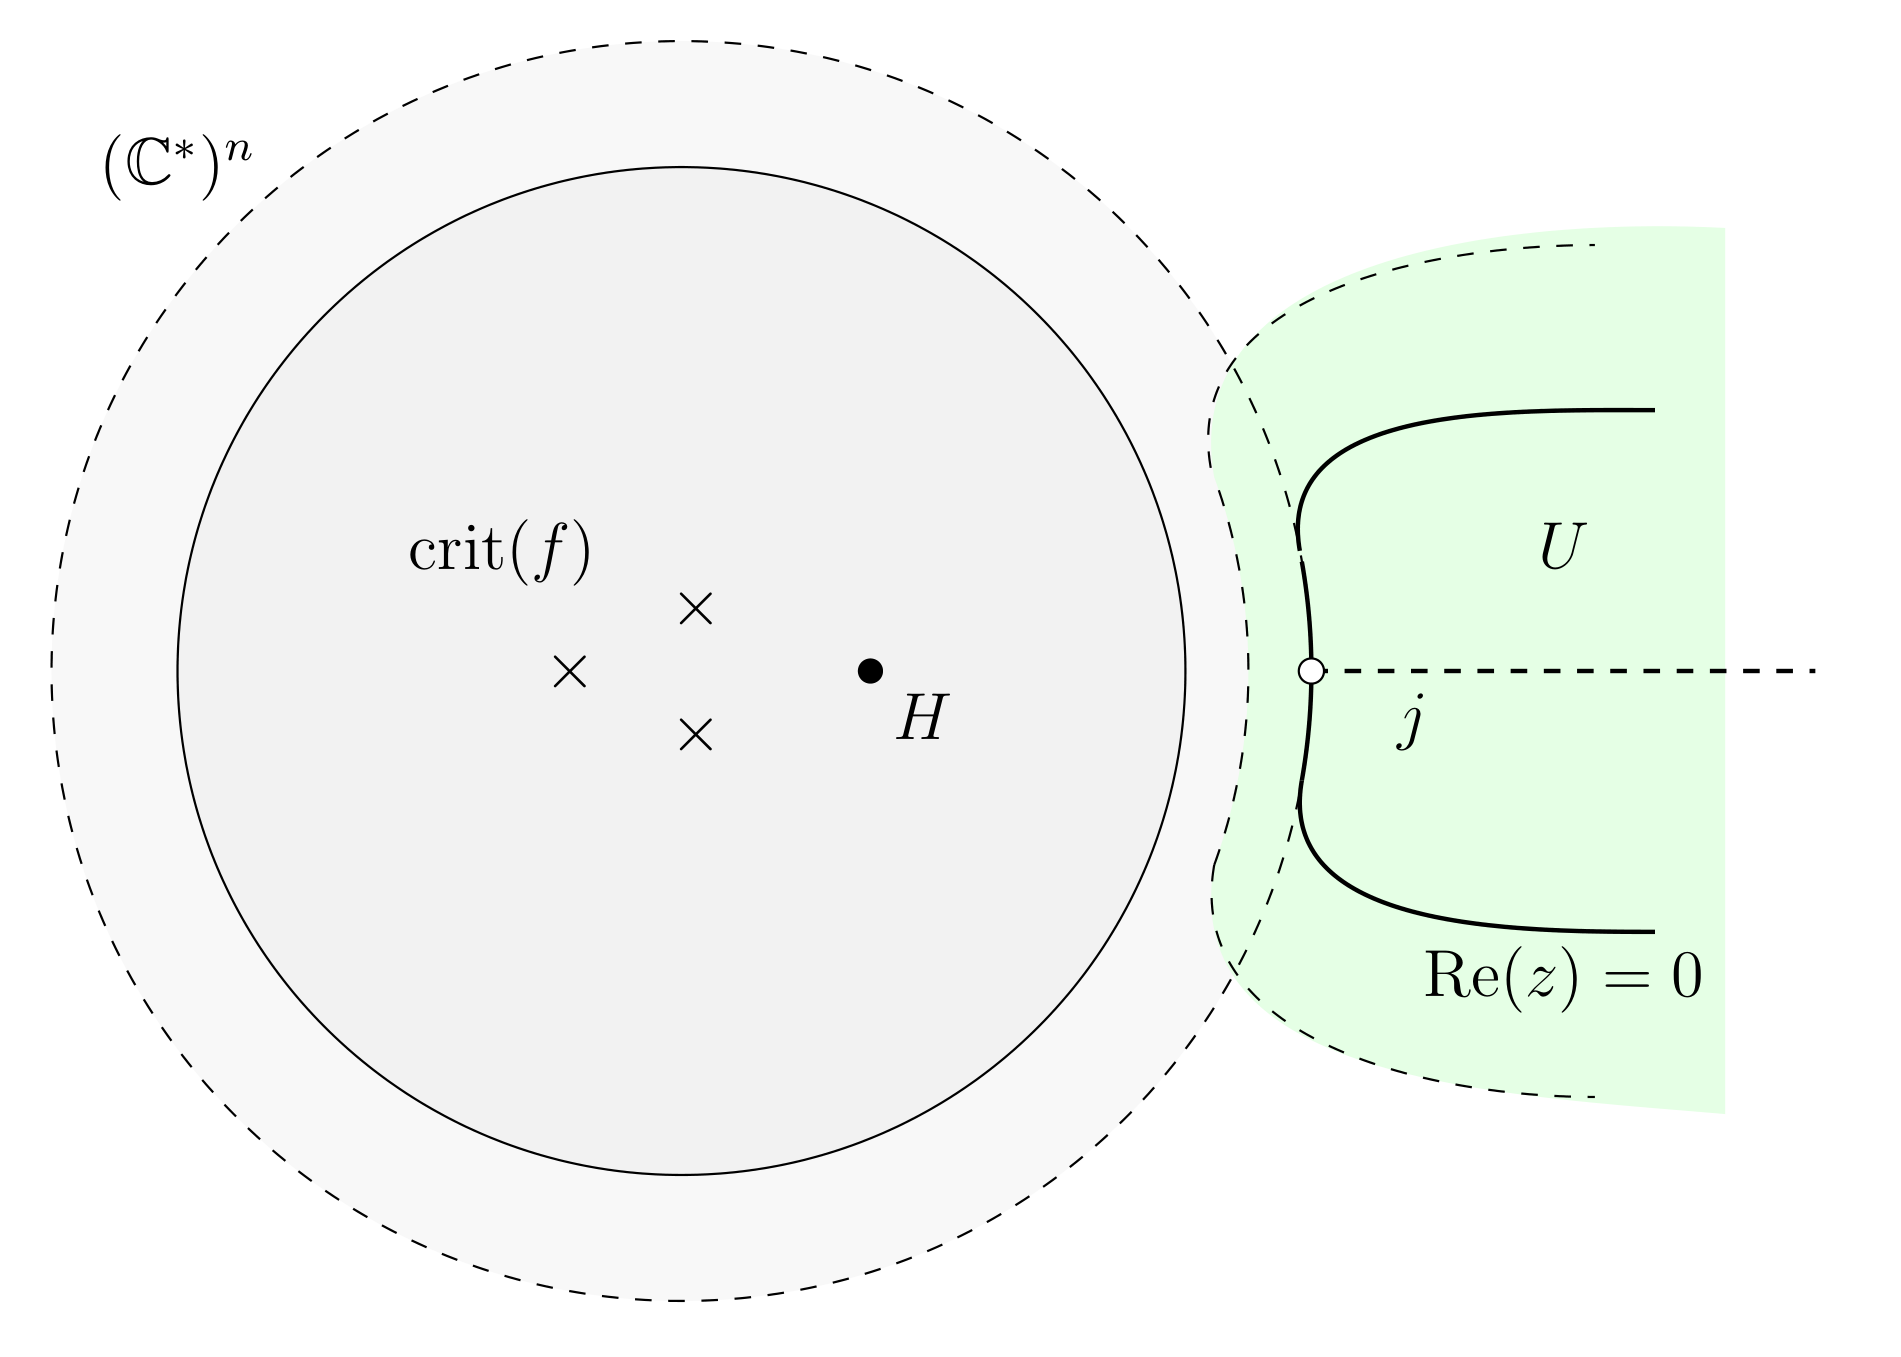
\includegraphics[width=0.52\textwidth]{figures/fig9_1.png}
\caption{提升函子 $j$ 对应于沿虚线水平线搬运拉格朗日对象：该虚线从穿孔出发，沿正实轴
延伸到 $\infty$。}
\label{fig:9-1}
\end{figure}

\begin{remarkx}
也可以定义负提升函子（negative lifting functor）
\[
j_-\colon\cW(H)\longrightarrow\cW(H\times A_1)\longrightarrow\cW((\C^*)^n\setminus H),
\]
其构造是：先与 $\R_{\le0}$ 作乘积并柱化，再作扇形包含（见图 \ref{fig:9-2}）。这一负提升
函子 $j_-$ 与提升函子 $j$ 相差一个扭转，即由 $f$ 绕 $\infty$ 的逆时针单值性 $\mu$ 给出的
扭转。
\end{remarkx}

\transnote{易错预警：原文在 $j_-$ 的中间范畴里写的是 $H\times A_1$，而在 $j$ 的定义里写的是
$H\times\C^*$；$A_1$ 在本节未另作说明，宜照原文录下，不要擅自改写成 $\R_{\le0}$——后者只
出现在紧随其后的柱化步骤中。}

\begin{theorem}\label{thm:9-0-2}
提升函子 $j\colon\cW(H)\to\cW_0((\C^*)^n\setminus H)$ 镜像于
\[
j_{D*}p_D^*\colon\operatorname{Coh}(D)\longrightarrow\operatorname{Coh}(Z),
\]
其中镜像等价取定理 \ref{thm:8-2-1} 中的 $\cW_0((\C^*)^n\setminus H)\to\operatorname{Coh}(Z)$；
这里 $j_D\colon K_X|_D\to Z$ 与 $p_D\colon K_X|_D\to D$ 分别是包含映射与投影。
\end{theorem}

% ===== 原书 p.130 =====

\begin{figure}[htbp]
\centering
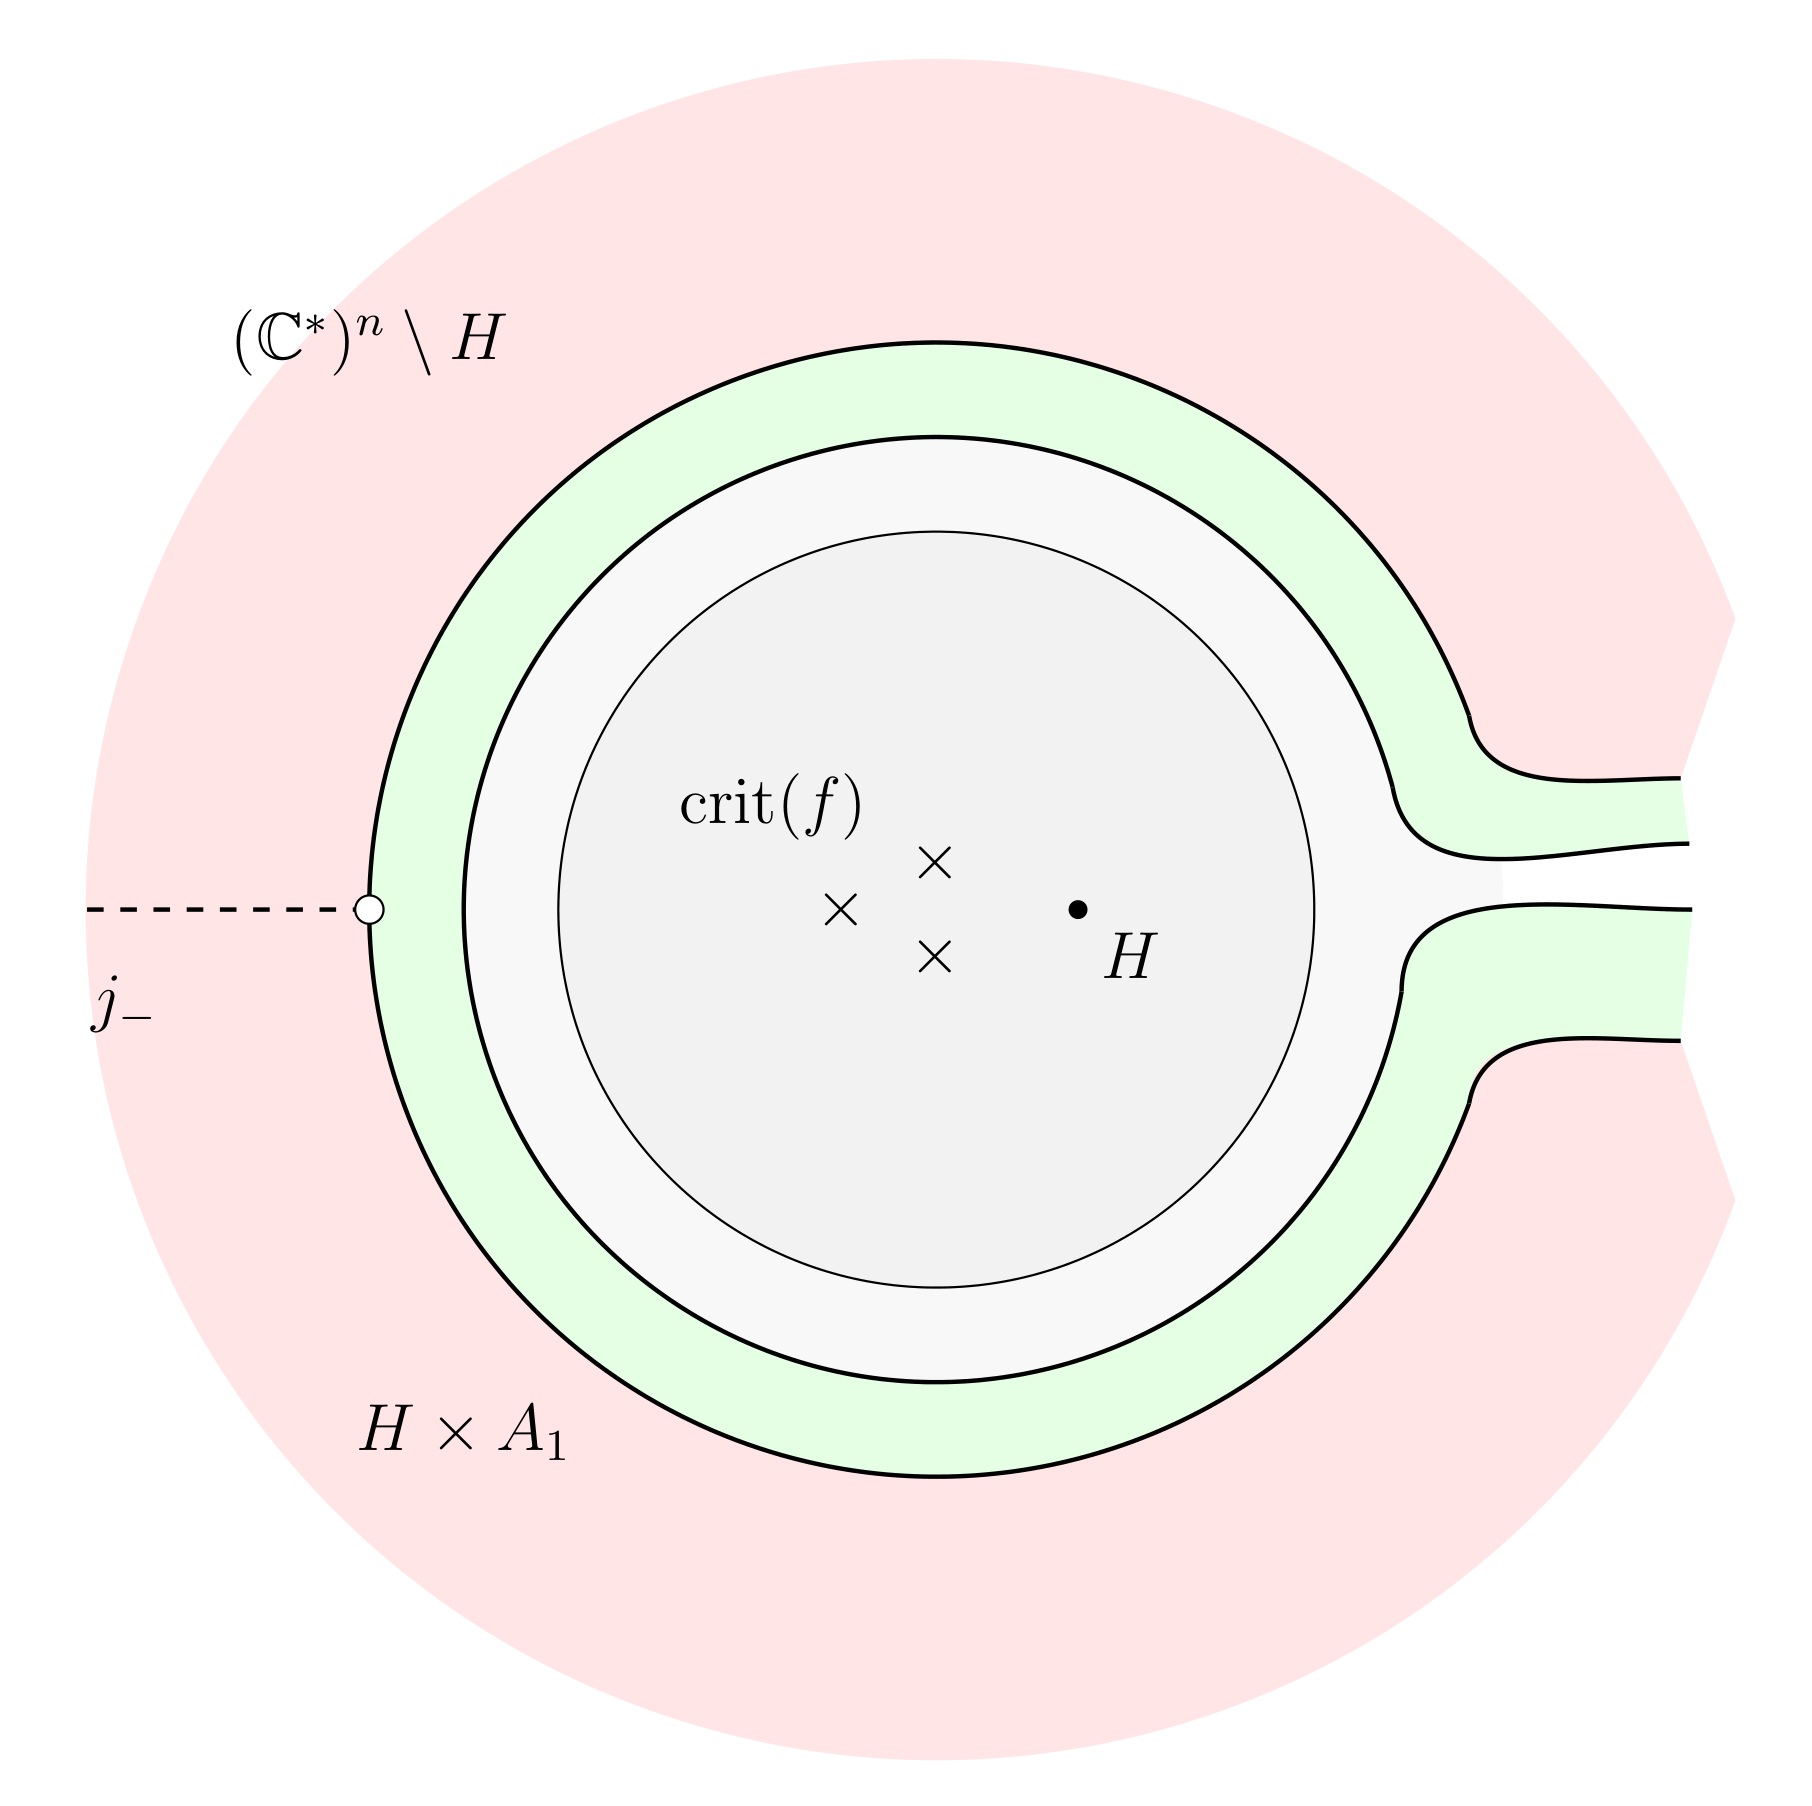
\includegraphics[width=0.42\textwidth]{figures/fig9_2.png}
\caption{负提升函子 $j_-$ 对应于沿虚线水平线搬运拉格朗日对象：该虚线从穿孔出发，延伸到
$-\infty$。}
\label{fig:9-2}
\end{figure}

% ===== 原书 p.131 =====

\begin{proof}
先考虑下面的图：
\[
\begin{tikzcd}[row sep=2.4em, column sep=1.5em]
\cW(H) \arrow[r,"\times\R_{\le0}"] \arrow[d,"\sim"] & \cW(H\times\C^*(2),z)
\arrow[r] \arrow[d,"\sim"] & \cW_0((\C^*)^n\setminus H) \arrow[d,"\sim"] \\
\operatorname{Coh}(D) \arrow[r,"p_{\tilde D}^*"] & \operatorname{Coh}(D\times\mathbb A^1[-1])
\arrow[r,"j_{\tilde D*}"] & \operatorname{Coh}(\tilde Z)
\end{tikzcd}
\]
右边的方块由定理 \ref{thm:7-2-4} 中的图而交换。左边的方块也交换，因为两个函子都对应于与
$\C[z]$（$|z|=2$）作张量。于是 $j\colon\cW(H)\to\cW_0((\C^*)^n\setminus H)$ 镜像于
$j_{\tilde D*}p_{\tilde D}^*\colon\operatorname{Coh}(D)\to\operatorname{Coh}(\tilde Z)$。
接下来由引理 \ref{lem:8-1-1}：在 Knörrer 等价 $\operatorname{Coh}(\tilde Z)\to
\operatorname{Coh}(Z)$ 之下，$j_{\tilde D*}p_{\tilde D}^*$ 再次被送到 $j_{D*}p_D^*$。
\end{proof}

\transnote{易错预警：交换图里带波浪号的箭头是范畴等价，不是同构的自然变换；同时注意
$\tilde D$ 与 $D$、$\tilde Z$ 与 $Z$ 的区别——定理的结论里落到的是不带波浪号的
$j_{D*}p_D^*$，带波浪号的那个只是证明中途的对象。}

\transnote{背景直觉：交换图里 $\C^*(2)$ 括号中的 2 表示该 $\C^*$ 因子的分次权重为 2，即其坐标 $z$ 满足 $|z|=2$；下文「与 $\C[z]$（$|z|=2$）作张量」正是对这一记号的说明。}

\begin{remarkx}
由于单值性带来的扭转，在 $\cW_0((\C^*)^n\setminus H)$ 与 $\operatorname{Coh}(Z)$ 的
镜像等价之下，负提升函子 $j_-$ 会镜像于 $j_{D*}p_D^*(K_X^{-1}|_D\otimes\cdot)$。理由如下：
由命题 \ref{prop:7-2-1}，逆时针单值性 $\mu$ 镜像于与 $K_X^{-1}|_D$ 作张量。这一结论对应于
猜想 \ref{conj:aur-funct} 的第 (4) 条。
\end{remarkx}

\transnote{易错预警：$K_X^{-1}|_D\otimes\cdot$ 表示先取 $K_X^{-1}$ 在 $D$ 上的限制，再与
对象作张量；它不是 $K_X^{-1}|_D$ 与某个固定对象的张量积，也不是 $K_X|_D$ 的逆。}

\begin{lemma}\label{lem:9-0-3}
存在 $\operatorname{Coh}(X)\to\operatorname{Coh}(Z)$ 的函子正合三角形：
\[
\begin{tikzcd}[row sep=1.0em, column sep=3.4em]
{j_{D*}p_D^*i_D^*} \arrow[rr,"+1"] & & i_{X*} \arrow[dl] \\
& \pi_X^* \arrow[ul] &
\end{tikzcd}
\]
\end{lemma}

\begin{proof}
映射 $i_{X*}\cF\to\pi_X^*\cF$ 是子层包含（subsheaf inclusion）：其余核恰是限制 $\cF|_D$ 沿投影
$K_X|_D\to D$ 的拉回。
\end{proof}

\transnote{含糊点拨：原文只画出三角形而未写循环方向。按本页的箭头读，它是
$\pi_X^*\to j_{D*}p_D^*i_D^*\xrightarrow{+1}i_{X*}\to\pi_X^*$；$+1$ 标在从第三个顶点
出发的那条箭头上，表示该映射带分次移位 1。}

\begin{corollary}\label{cor:9-0-4}
存在正合三角形，把作为函子 $\cW((\C^*)^n,f)\to\cW_\infty((\C^*)^n\setminus H)$ 的
$\alpha_0$、$\alpha_\infty$ 与 $j\cap$ 联系起来：

% ===== 原书 p.132 =====

\[
\begin{tikzcd}[row sep=1.0em, column sep=3.4em]
{j\cap} \arrow[rr,"+1"] & & \alpha_0 \arrow[dl] \\
& \alpha_\infty \arrow[ul] &
\end{tikzcd}
\]
并且对 $\cW_0((\C^*)^n\setminus H)$ 与 $j_-$ 有相应的正合三角形。
\end{corollary}

\transnote{易错预警：本三角形的三个顶点排布是 $j\cap$、$\alpha_0$（右上）、$\alpha_\infty$
（下方）。按箭头读，循环为 $\alpha_\infty\to j\cap\xrightarrow{+1}\alpha_0\to\alpha_\infty$。
不要与 §1.6 中同型三角形的排布混看，那里 $\alpha_0$ 与 $\alpha_\infty$ 的位置相反。}

\begin{proof}
这正是引理 \ref{lem:9-0-3} 的镜像：用定理 \ref{thm:8-2-1} 可知 $\pi_X^*$ 镜像于
$\alpha_\infty$。
\end{proof}

\subsection{一个例子}

本节的例子取 $H=\{-1\}$，篇幅虽短，却足以显示 $[1]$-移位与不同 $\Z$-分次为何必要。
先在 B 侧作如下等同：
\begin{itemize}[leftmargin=2em,itemsep=0.2em]
\item $X=\operatorname{Spec}(\C[x])$；
\item $K_X=\operatorname{Spec}(\C[x,y])$；
\item $\mathbb A^1[-1]=\operatorname{Spec}(\C[t])$，$|t|=-1$。
\end{itemize}

在 A 侧，$\Pi_1=\C^*\setminus H$ 有两种不同的粘合展示，分别由命题 \ref{prop:7-1-1} 与
命题 \ref{prop:7-1-2} 给出，如图 \ref{fig:9-3} 所示。此时两种分次的选择容易描述：
\[
\eta_0=\frac{\dd z}{z},\qquad\qquad \eta_\infty=\frac{\dd z}{z(z+1)}.
\]
对 $\eta_0$ 而言，绕 $-1$ 的简单顺时针 Reeb 轨道次数为 2，绕另外两个穿孔的相应轨道次数
为 0。

% ===== 原书 p.133 =====

\begin{figure}[htbp]
\centering
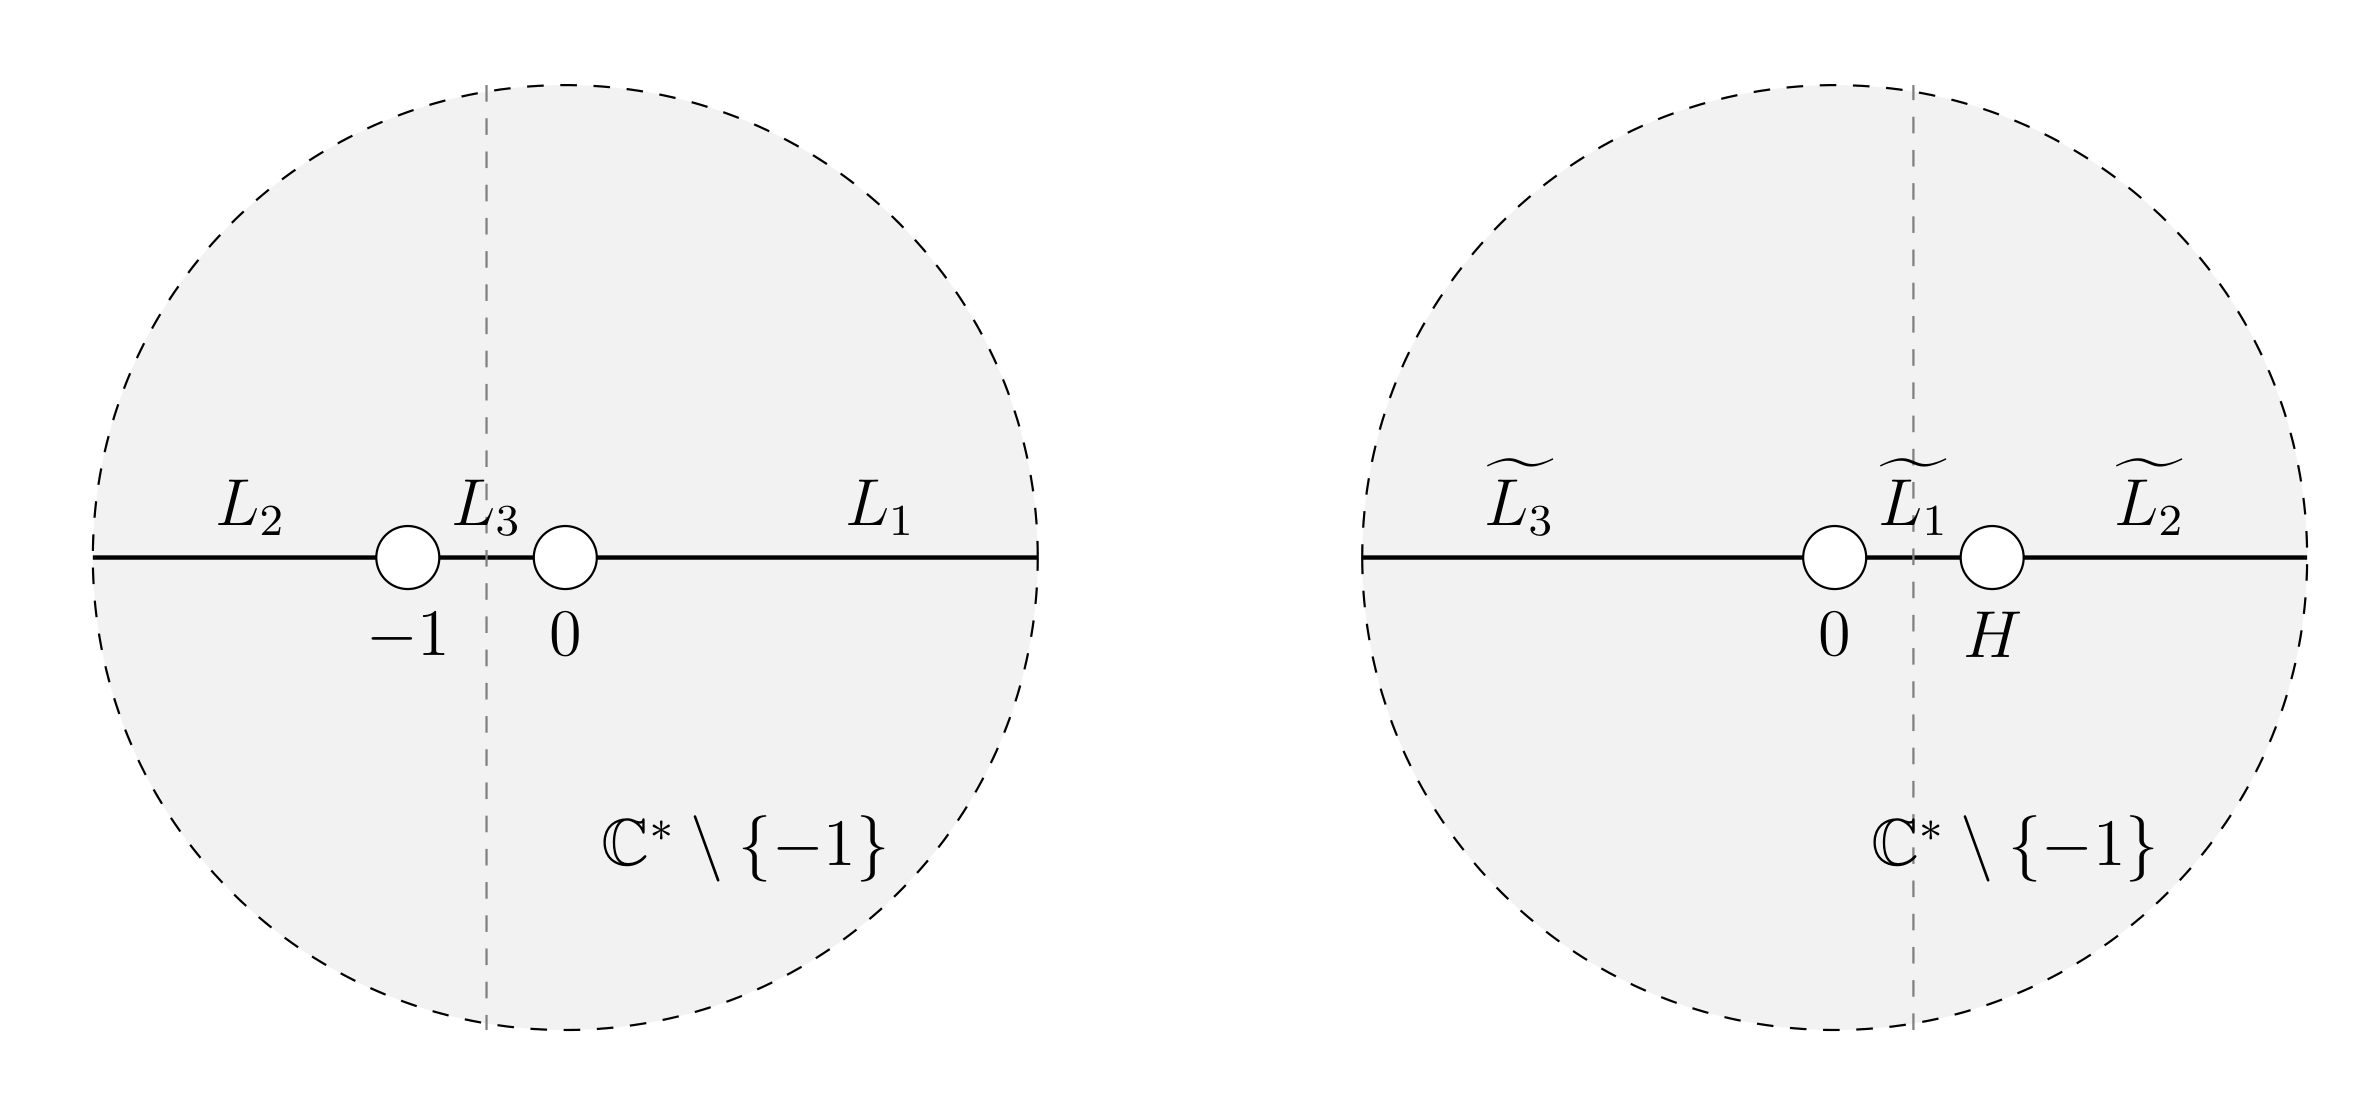
\includegraphics[width=0.78\textwidth]{figures/fig9_3.png}
\caption{裤子（pair of pants）的两种粘合展示，分别来自 $\tilde f_0$ 与 $\tilde f_\infty$
（从左到右），图中标出生成拉格朗日对象。虚线竖线表示划分两个子扇形的扇形超曲面。}
\label{fig:9-3}
\end{figure}

对 $\eta_\infty$ 则情形相反：绕 $\infty$ 的简单顺时针 Reeb 轨道次数为 2。希望这能部分
解释我们所选取的记号。这也提示：在不太正式的意义上，等价
$\cW_0(\Pi_1)\to\cW_\infty(\Pi_1)$ 会「交换零与无穷」。

\transnote{易错预警：$\eta_0$ 与 $\eta_\infty$ 是同一个补集上两个不同的平凡化，因而给出
两个\emph{不同的} dg 范畴 $\cW_0(\Pi_1)$ 与 $\cW_\infty(\Pi_1)$；下标 0、$\infty$ 指的是
分次所用平凡化，不是某种极限。}

如图 \ref{fig:9-3} 所示，我们用 $L_1,L_2,L_3$ 记取 0-分次的 wrapped Fukaya 范畴的一组
生成拉格朗日对象（generating Lagrangians），用 $\tilde L_1,\tilde L_2,\tilde L_3$ 记取 $\infty$-分次的相应对象。
事实上可以证明：与 Knörrer 周期性等价 $\operatorname{Coh}(Z)\to\operatorname{Coh}(\tilde Z)$
复合，会把 $L_i$ 与 $\tilde L_i$ 互换。特别地，$j_-$ 将对应于 $j$；一般情形下，这会涉及
单值性的扭转。

\transnote{含糊点拨：“$j_-$ 将对应于 $j$”是一句简写：两者的镜像只在复合 Knörrer 等价并
作单值性扭转之后才一致。原文紧接的“一般情形下”正是指这个扭转，读时不要理解成 $j_-=j$。}

\begin{proposition}\label{prop:9-1-1}
在定理 \ref{thm:7-2-4} 与定理 \ref{thm:8-2-1} 所诱导的镜像对称等价之下，有
\begin{itemize}[leftmargin=2em,itemsep=0.2em]
\item $\alpha_\infty(L_1)\mapsto\pi_{\mathbb A^1_x}^*(\cO_{\mathbb A^1_x})[1]$，

% ===== 原书 p.134 =====

\item $\alpha_0(\tilde L_2)\mapsto i_{\mathbb A^1_x*}(\cO_{\mathbb A^1_x})$，
\item $\rho(L_2)\mapsto q(\cO_{\mathbb A^1_y})$；
\item $j(\C)\mapsto\pi_{\mathbb A^1_y}^*(\cO_0)$。
\end{itemize}
\end{proposition}

\transnote{易错预警：这一组公式里 $\mathbb A^1_x$ 与 $\mathbb A^1_y$ 的下标并不统一——前
两条用 $x$，后两条用 $y$。这是原文的写法，照录；不要把它们“统一”成同一个坐标。}

\begin{proof}
按定义，$\alpha_\infty$ 把 $\cW(\C^*,z)$ 的唯一生成元 $L_1$ 送到 $\cW_0(\Pi_1)$ 中的
$L_1$；同样，$\alpha_0$ 把 $\cW(\C^*,z)$ 的生成元送到 $\cW_\infty(\Pi_1)$ 中的
$\tilde L_2$。在粘合诱导的镜像等价之下，前者被送到模 $\C[x]$ 到
$\mathbb A^1\cup_0\mathbb A^1[-1]=\tilde Z$ 的推出。同样，$\tilde L_2$ 作为
$\C[x,y]/(xy)$-模对应于 $\C[x]$，这就验证了 $\alpha_0$ 与 $i_{X*}$ 的对应。

接下来需要理解 Knörrer 周期性等价
\[
\operatorname{Coh}\C[x,y]/(xy)\longrightarrow
\operatorname{Coh}_{\mathbb G_m}(\mathbb A^1\times\mathbb A^1\times\mathbb A^1,xyt)
\longleftarrow\operatorname{Coh}\C[x,t]/(xt).
\]
在这一等价下，$\operatorname{Coh}(\mathbb A^1\cup_0\mathbb A^1[-1])$ 中的 $\C[x]$ 被送到
下面的矩阵分解：
\[
\begin{tikzcd}[row sep=1.4em, column sep=5em]
\C[x,y,t] \arrow[rr,bend left=20,"t"] & & \C[x,y,t] \arrow[ll,bend left=20,"xy"']
\end{tikzcd}
\]
它是下列矩阵分解的 $[1]$-移位：
\[
\begin{tikzcd}[row sep=1.4em, column sep=5em]
\C[x,y,t] \arrow[rr,bend left=20,"xy"] & & \C[x,y,t] \arrow[ll,bend left=20,"t"']
\end{tikzcd}
\]
而后者又是 $\operatorname{Coh}(\mathbb A^1\cup_0\mathbb A^1)$ 中 $\C[x,y]/(xy)$ 的像
（注意 $t$ 的权为 1 这一点要紧）。这一模沿投影 $\mathbb A^1\cup_0\mathbb A^1\to\mathbb A^1$
从 $\operatorname{Coh}(X)$ 的生成元 $\C[x]$ 拉回。
\end{proof}

\transnote{含糊点拨：两幅来回箭头的图是矩阵分解的简写——一对模配上两条映射。前一幅的
上方箭头为 $t$、下方箭头为 $xy$，后一幅把二者对调；对调恰是 $[1]$-移位的效果，因此文中
说前者是后者的 $[1]$-移位。}

\clearpage
% EN49 c13 | 原书 p.135–145（PDF 146–156）| 承接上块命题之证明 + 附录 A 记号 + 参考文献
% 每页起首以 % ===== 原书 p.N ===== 注释标记。

% ===== 原书 p.135 =====

\begin{proof}[命题 \ref{prop:9-1-1} 的证明（续）]
于是我们在这一系列等同之下已经证明：$\alpha_\infty(L_1)$ 对应于 $\pi_X^*(\cO_X)[1]$。

验证函子 $\rho$ 的镜像等价同样简单。限制函子 $\rho$ 把 $L_2$ 送到 $\C$；而在我们的
粘合构造所给出的镜像对称等价之下，$L_2$ 对应于 $\operatorname{Coh}(\mathbb A^1\cup_0
\mathbb A^1[-1])$ 中的 $\C[t]$。注意 $\C[t]$ 的自同态代数是 $\C[x,z]/(xz)$，$|z|=2$，
与 $L_2$ 的情形相同。把这一模过一遍 Knörrer 周期性，得到 $\C[x,y]/(xy)$-模 $\C[y]$；
它在商映射（quotient map）到 $\operatorname{Sing}(\C[x,y]/(xy))$ 之下确实映到 $\C$。同样，提升函子
$j$ 的像是 $L_2$，而如前所见，它对应于 $\C[y]$，即 $\cO_0$ 沿投影
$\mathbb A^1\cup_0\mathbb A^1\to\mathbb A^1$ 的拉回。
\end{proof}

\transnote{背景直觉：这一句里的 $[1]$ 不可省。命题 \ref{prop:9-1-1} 四条对应中只有
$\alpha_\infty(L_1)$ 与 $j(\C)$ 带这个移位，它正是 $\alpha_\infty$ 与 $\alpha_0$ 在分次上
错开一级的体现。}

\transnote{易错预警：本段的 $z$ 有两个来源。$\C[x,z]/(xz)$ 里的 $z$ 是新增的环变量
（$|z|=2$）；而 §9.1 开头 $\cW(\C^*,z)$ 里的 $z$ 是 $\C^*$ 的坐标。两处同字母，含义不同。}

\transnote{含糊点拨：句中两次出现的 $L_2$ 说的是同一对象的两张面孔：$\rho$ 把它送到 $\C$
（A 侧的限制像），镜像等价又把它送到 $\C[t]$（B 侧的模）。不要读成两个不同的对象。}

\transnote{易错预警：过 Knörrer 周期性时变量名从 $t$ 换成 $y$，即 $\C[t]$ 变成 $\C[y]$。
这是同一条对应链上的两种写法，不是两个不同的对象。}

\section*{附录 A\quad 记号}
\addcontentsline{toc}{section}{附录 A\quad 记号}

% ===== 原书 p.136 =====

我们在此列出全文用到的概型间态射，以便查检：先列包含映射：
\begin{itemize}[leftmargin=2em,itemsep=0.25em]
\item $i_D\colon D\to X$；$i_Z\colon Z\to K_X$；
$i_{\tilde Z}\colon\tilde Z\to X\times\mathbb A^1[-1]$，
$i_{\hat Z}\colon\hat Z\to K_X\times\mathbb A^1$，$i_X\colon X\to Z$，
$i_{\tilde X}\colon X\to\tilde Z$；
\item $j_D\colon K_X|_D\to Z$，$j_{\tilde D}\colon D\times\mathbb A^1[-1]\to\tilde Z$，
$j_Z\colon Z\times\mathbb A^1[-1]\to\hat Z$；
$j_{\tilde Z}\colon K_{X\times\mathbb A^1}|_{\tilde Z}\to\hat Z$；
\item $\iota_{\tilde D}\colon D\to D\times\mathbb A^1[-1]$；
$\iota_D\colon D\to K_X|_D$；$\iota_Z\colon Z\to Z\times\mathbb A^1[-1]$；
$\iota_{\tilde Z}\colon\tilde Z\to K_{X\times\mathbb A^1}|_{\tilde Z}$；
\item $\iota_X\colon X\to K_X$；$\iota_{\tilde X}\colon X\to X\times\mathbb A^1[-1]$；
$\iota_{K_X}\colon K_X\to K_X\times\mathbb A^1[-1]$；
$\iota_{X\times\mathbb A^1[-1]}\colon X\times\mathbb A^1[-1]\to K_X\times\mathbb A^1[-1]$。
\end{itemize}
然后是投影：
\begin{itemize}[leftmargin=2em,itemsep=0.25em]
\item $p_D\colon K_X|_D\to D$；$p_{\tilde D}\colon D\times\mathbb A^1[-1]\to D$；
$p_Z\colon Z\times\mathbb A^1[-1]\to Z$；
$p_{\tilde Z}\colon K_{X\times\mathbb A^1}|_{\tilde Z}\to\tilde Z$；
\item $\pi_Z\colon K_X\times\mathbb A^1[-1]\to K_X$；
$\pi_{\tilde Z}\colon K_X\times\mathbb A^1[-1]\to X\times\mathbb A^1[-1]$；
$\pi_X\colon Z\to X$，$\pi_{\tilde X}\colon\tilde Z\to X$。
\end{itemize}

\transnote{背景直觉：本附录按“包含映射（inclusions）—投影（projections）”两组罗列全书
用到的概型态射，读者可凭定义域与目标认出箭头。这些记号与 §1.5 中 $Z$、$\tilde Z$、
$\hat Z$ 等构造配套使用。}

\transnote{易错预警：$\tilde Z$、$\hat Z$、$\tilde S$ 只差一个重音符号，切勿混同。
$\tilde Z$ 是把 $X\times\{0\}$ 沿 $D$ 粘到 $D\times\mathbb A^1[-1]$ 所得的导出概型；
$\hat Z$ 是 $K_X\times\mathbb A^1$ 内的反典范除子；$\tilde S$ 是 $X\times\mathbb A^1$ 内的
反典范除子。}

\transnote{易错预警：$K_X$ 与 $\cK_X$ 不同。$K_X$ 是典范丛的全空间（一个概型），
$\cK_X$ 是典范层；表中出现的 $K_X|_D$ 指全空间沿 $D$ 的限制，于是它本身仍是概型，
$j_D\colon K_X|_D\to Z$ 才有意义。}

% ===== 原书 p.137 =====

以及经典概型（classical scheme）$\tilde S$ 的类似情形。

\transnote{含糊点拨：原文只写“经典概型 $\tilde S$ 的情形同理”，未逐条列出。$\tilde S$ 是
$X\times\mathbb A^1$ 内的（经典）反典范除子，与之配套的箭头可由本表逐条类比得到。}

\section*{参考文献}
\addcontentsline{toc}{section}{参考文献}

% ===== 原书 p.138 =====

\begingroup
\parindent=0pt
\parskip=0.55em plus 0.2em
\raggedright

[AA21] Mohammed Abouzaid and Denis Auroux, \emph{Homological mirror symmetry for
hypersurfaces in $(\C^*)^n$}, 2021, preprint: arXiv:2111.06543.

[AAK16] Mohammed Abouzaid, Denis Auroux, and Ludmil Katzarkov, \emph{Lagrangian
fibrations on blowups of toric varieties and mirror symmetry for hypersurfaces},
Publ.\ Math.\ Inst.\ Hautes \'Etudes Sci.\ \textbf{123} (2016), 199--282.
MR 3502098

[Abo06] Mohammed Abouzaid, \emph{Homogeneous coordinate rings and mirror symmetry for
toric varieties}, Geom.\ Topol.\ \textbf{10} (2006), 1097--1156. MR 2240909

[Abo09] \rule[0.4ex]{2.6em}{0.4pt} , \emph{Morse homology, tropical geometry, and
homological mirror symmetry for toric varieties}, Selecta Math.\ (N.S.)\ \textbf{15}
(2009), no.~2, 189--270. MR 2529936

[Abo17] \rule[0.4ex]{2.6em}{0.4pt} , \emph{The family Floer functor is faithful},
J.\ Eur.\ Math.\ Soc.\ (JEMS)\ \textbf{19} (2017), no.~7, 2139--2217. MR 3656481

[AG] Mohammed Abouzaid and Sheel Ganatra, \emph{Generating Fukaya categories of LG
models}, to appear.

[AG15] D. Arinkin and D. Gaitsgory, \emph{Singular support of coherent sheaves and the
geometric Langlands conjecture}, Selecta Math.\ (N.S.)\ \textbf{21} (2015), no.~1,
1--199. MR 3300415

[AKO06] Denis Auroux, Ludmil Katzarkov, and Dmitri Orlov, \emph{Mirror symmetry for del
Pezzo surfaces: vanishing cycles and coherent sheaves}, Invent.\ Math.\ \textbf{166}
(2006),

% ===== 原书 p.139 =====

no.~3, 537--582. MR 2257391

[AS] Mohammed Abouzaid and Paul Seidel, \emph{Lefschetz fibration methods in wrapped
Floer theory}, to appear.

[AS15] Mohammed Abouzaid and Ivan Smith, \emph{Khovanov homology from Floer
cohomology}, preprint: arXiv:1504.01230, 2015.

[Aur18] Denis Auroux, \emph{Speculations on homological mirror symmetry for
hypersurfaces in $(\C^*)^n$}, Surveys in differential geometry 2017, Surv.\ Differ.\
Geom., vol.~22, Int.\ Press, Somerville, MA, 2018, pp.~1--47. MR 3838112

[BC17] Paul Biran and Octav Cornea, \emph{Cone-decompositions of Lagrangian cobordisms
in Lefschetz fibrations}, Selecta Math.\ (N.S.)\ \textbf{23} (2017), no.~4,
2635--2704. MR 3703462

[BCS05] Lev A. Borisov, Linda Chen, and Gregory G. Smith, \emph{The orbifold Chow ring
of toric Deligne-Mumford stacks}, J.\ Amer.\ Math.\ Soc.\ \textbf{18} (2005), no.~1,
193--215. MR 2114820

[Can20] Catherine Cannizzo, \emph{Categorical mirror symmetry on cohomology for a
complex genus 2 curve}, Advances in Mathematics \textbf{375} (2020), 107392.

[CE12] Kai Cieliebak and Yakov Eliashberg, \emph{From Stein to Weinstein and back},
American Mathematical Society Colloquium Publications, vol.~59, American Mathematical
Society, Providence, RI, 2012, Symplectic geometry of affine complex manifolds.
MR 3012475

[FLTZ12] Bohan Fang, Chiu-Chu Melissa Liu, David Treumann, and Eric Zaslow,
\emph{T-duality and homological mirror symmetry for toric varieties}, Adv.\ Math.\
\textbf{229} (2012), no.~3, 1875--1911. MR 2871160

[FSS08] Kenji Fukaya, Paul Seidel, and Ivan Smith, \emph{Exact Lagrangian submanifolds
in simply-connected cotangent bundles}, Invent.\ Math.\ \textbf{172} (2008), no.~1,
1--27. MR 2385665

% ===== 原书 p.140 =====

[Fuk02] Kenji Fukaya, \emph{Mirror symmetry of abelian varieties and multi-theta
functions}, J.\ Algebraic Geom.\ \textbf{11} (2002), no.~3, 393--512. MR 1894935

[Gam20] Benjamin Gammage, \emph{Mirror symmetry for Berglund-H{\"u}bsch Milnor fibers},
2020, preprint: arxiv:2010.15570.

[GJ22] Benjamin Gammage and Maxim Jeffs, \emph{Functorial mirror symmetry for very
affine hypersurfaces}, 2022, preprint: arxiv:2210.03227.

[GKR17] Mark Gross, Ludmil Katzarkov, and Helge Ruddat, \emph{Towards mirror symmetry
for varieties of general type}, Adv.\ Math.\ \textbf{308} (2017), 208--275. MR 3600059

[GPS19] Sheel Ganatra, John Pardon, and Vivek Shende, \emph{Sectorial descent for
wrapped Fukaya categories}, preprint: arxiv:1809.03427, 2019.

[GPS20a] \rule[0.4ex]{2.6em}{0.4pt} , \emph{Covariantly functorial wrapped Floer theory
on Liouville sectors}, Publ.\ Math.\ Inst.\ Hautes \'Etudes Sci.\ \textbf{131} (2020),
73--200.

[GPS20b] \rule[0.4ex]{2.6em}{0.4pt} , \emph{Covariantly functorial wrapped Floer theory
on Liouville sectors}, Publ.\ Math.\ Inst.\ Hautes \'Etudes Sci.\ \textbf{131} (2020),
73--200. MR 4106794

[GPS20c] Sheel Ganatra, John Pardon, and Vivek Shende, \emph{Microlocal Morse theory of
wrapped Fukaya categories}, 2020, preprint: arxiv:1809.08807.

[GR17] Dennis Gaitsgory and Nick Rozenblyum, \emph{A study in derived algebraic
geometry. Vol. I. Correspondences and duality}, Mathematical Surveys and Monographs,
vol.~221, American Mathematical Society, Providence, RI, 2017. MR 3701352

[GS03] Mark Gross and Bernd Siebert, \emph{Affine manifolds, log structures, and mirror
symmetry}, Turk.\ J.\ Math.\ \textbf{27} (2003), no.~1, 33--60 (English).

[GS06] Mark Gross and Bernd Siebert, \emph{Mirror symmetry via logarithmic degeneration
data. I}, J.\ Differential Geom.\ \textbf{72} (2006), no.~2, 169--338. MR 2213573

% ===== 原书 p.141 =====

[GS10] \rule[0.4ex]{2.6em}{0.4pt} , \emph{Mirror symmetry via logarithmic degeneration
data, II}, J.\ Algebraic Geom.\ \textbf{19} (2010), no.~4, 679--780. MR 2669728

[GS16] \rule[0.4ex]{2.6em}{0.4pt} , \emph{Theta functions and mirror symmetry}, Surveys
in differential geometry 2016. Advances in geometry and mathematical physics, Surv.\
Differ.\ Geom., vol.~21, Int.\ Press, Somerville, MA, 2016, pp.~95--138. MR 3525095

[GS21] Benjamin Gammage and Vivek Shende, \emph{Homological mirror symmetry at large
volume}, 2021, preprint: arxiv:2104.11129.

[GS22] \rule[0.4ex]{2.6em}{0.4pt} , \emph{Mirror symmetry for very affine hypersurfaces},
2022, To appear.

[Han19] Andrew Hanlon, \emph{Monodromy of monomially admissible Fukaya-Seidel categories
mirror to toric varieties}, Adv.\ Math.\ \textbf{350} (2019), 662--746. MR 3948684

[HH22] A. Hanlon and J. Hicks, \emph{Aspects of functoriality in homological mirror
symmetry for toric varieties}, Adv.\ Math.\ \textbf{401} (2022), Paper No.~108317.
MR 4394684

[Hir17] Yuki Hirano, \emph{Derived Kn{\"o}rrer periodicity and Orlov's theorem for
gauged Landau-Ginzburg models}, Compos.\ Math.\ \textbf{153} (2017), no.~5, 973--1007.
MR 3631231

[HK21] Paul Hacking and Ailsa Keating, \emph{Symplectomorphisms of mirrors to log
Calabi-Yau surfaces}, 2021, preprint: arxiv:2112.06797.

[HV00] Kentaro Hori and Cumrun Vafa, \emph{Mirror symmetry}, 2000, preprint:
arXiv:hep-th/0002222.

[Jef22] Maxim Jeffs, \emph{Mirror symmetry and Fukaya categories of singular
hypersurfaces}, Advances in Mathematics \textbf{397} (2022), 108116.

[Joy15] Dominic Joyce, \emph{A classical model for derived critical loci}, J.\
Differential Geom.\ \textbf{101} (2015), no.~2, 289--367. MR 3399099

[KM98] J{\'a}nos Koll{\'a}r and Shigefumi Mori, \emph{Birational geometry of algebraic
varieties}, Cambridge Tracts in Mathematics, vol.~134, Cambridge University Press,
Cambridge, 1998, With the collaboration of C. H. Clemens and A. Corti, Translated from
the 1998 Japanese original. MR 1658959

% ===== 原书 p.142 =====

[Kon95] Maxim Kontsevich, \emph{Homological algebra of mirror symmetry}, Proceedings of
the International Congress of Mathematicians (Basel) (S. D. Chatterji, ed.),
Birkh{\"a}user Basel, 1995, pp.~120--139.

[KS14a] Mikhail Kapranov and Vadim Schechtman, \emph{Perverse schobers}, 2014, preprint:
arXiv:1411.2772.

[KS14b] \rule[0.4ex]{2.6em}{0.4pt} , \emph{Perverse schobers}, preprint:
arxiv:1411.2772, 2014.

[Kuw20] Tatsuki Kuwagaki, \emph{The nonequivariant coherent-constructible correspondence
for toric stacks}, Duke Math.\ J.\ \textbf{169} (2020), no.~11, 2125--2197. MR 4132582

[LO06] Volodymyr Lyubashenko and Sergiy Ovsienko, \emph{A construction of quotient
$A_\infty$-categories.}, Homology Homotopy Appl.\ \textbf{8} (2006), no.~2, 157--203
(English).

[LP12] Yank{\i} Lekili and Timothy Perutz, \emph{Arithmetic mirror symmetry for the
2-torus}, preprint: arXiv:1211.4632, 2012.

[LP17] Yank{\i} Lekili and Alexander Polishchuk, \emph{Arithmetic mirror symmetry for
genus 1 curves with $n$ marked points}, Selecta Math.\ (N.S.)\ \textbf{23} (2017),
no.~3, 1851--1907. MR 3663596

[Mum72] David Mumford, \emph{An analytic construction of degenerating curves over
complete local rings}, Compositio Math.\ \textbf{24} (1972), 129--174. MR 352105

[Nad17] David Nadler, \emph{A combinatorial calculation of the Landau-Ginzburg model
$M=\C^3$, $W=z_1z_2z_3$}, Selecta Math.\ (N.S.)\ \textbf{23} (2017), no.~1, 519--532.
MR 3595901

[Nad19a] \rule[0.4ex]{2.6em}{0.4pt} , \emph{Mirror symmetry for the Landau-Ginzburg
A-model $M=\C^n$, $W=z_1\cdots z_n$}, Duke Math.\ J.\ \textbf{168} (2019), no.~1,
1--84. MR 3909893

% ===== 原书 p.143 =====

[Nad19b] David Nadler, \emph{Mirror symmetry for the Landau--Ginzburg A-model $M=\C^n$,
$W=z_1\cdots z_n$}, Duke Mathematical Journal \textbf{168} (2019), no.~1, 1--84.

[Orl06a] D. O. Orlov, \emph{Triangulated categories of singularities, and equivalences
between Landau-Ginzburg models}, Mat.\ Sb.\ \textbf{197} (2006), no.~12, 117--132.
MR 2437083

[Orl06b] Dmitri Orlov, \emph{Triangulated categories of singularities, and equivalences
between Landau-Ginzburg models}, Mat.\ Sb.\ \textbf{197} (2006), no.~12, 117--132.
MR 2437083

[Orl09a] \rule[0.4ex]{2.6em}{0.4pt} , \emph{Derived categories of coherent sheaves and
triangulated categories of singularities}, Algebra, arithmetic, and geometry: in honor
of Yu. I. Manin. Vol. II, Progr.\ Math., vol.~270, Birkh{\"a}user Boston, Boston, MA,
2009, pp.~503--531. MR 2641200

[Orl09b] \rule[0.4ex]{2.6em}{0.4pt} , \emph{Remarks on generators and dimensions of
triangulated categories}, Mosc.\ Math.\ J.\ \textbf{9} (2009), no.~1, 153--159, back
matter. MR 2567400

[Par12] Brett Parker, \emph{Log geometry and exploded manifolds}, Abh.\ Math.\ Semin.\
Univ.\ Hambg.\ \textbf{82} (2012), no.~1, 43--81. MR 2922725

[PS22] James Pascaleff and Nicol{\`o} Sibilla, \emph{Singularity categories of normal
crossings surfaces, descent, and mirror symmetry}, 2022, preprint: arxiv:2208.03896.

[PZ98] Alexander Polishchuk and Eric Zaslow, \emph{Categorical mirror symmetry: the
elliptic curve}, Adv.\ Theor.\ Math.\ Phys.\ \textbf{2} (1998), no.~2, 443--470.
MR 1633036

[PZ01] Alexander Polishchuk and Eric Zaslow, \emph{Categorical mirror symmetry in the
elliptic curve.}, Proceedings of the winter school on mirror symmetry, Cambridge, MA,
USA, January 1999, Providence, RI: American Mathematical Society (AMS); Somerville,
MA: International Press, 2001, pp.~275--295.

[Sei98] Paul Seidel, 1998, unpublished notes.

[Sei02] \rule[0.4ex]{2.6em}{0.4pt} , \emph{Fukaya categories and deformations},
Proceedings of the International Congress of Mathematicians, Vol. II (Beijing, 2002),
Higher Ed. Press, Beijing, 2002, pp.~351--360. MR 1957046

% ===== 原书 p.144 =====

[Sei08a] \rule[0.4ex]{2.6em}{0.4pt} , \emph{$A_\infty$-subalgebras and natural
transformations}, Homology Homotopy Appl.\ \textbf{10} (2008), no.~2, 83--114.
MR 2426130

[Sei08b] \rule[0.4ex]{2.6em}{0.4pt} , \emph{Fukaya categories and Picard-Lefschetz
theory}, Zurich Lectures in Advanced Mathematics, European Mathematical Society (EMS),
Z{\"u}rich, 2008.

[Sei09a] \rule[0.4ex]{2.6em}{0.4pt} , \emph{Suspending Lefschetz fibrations, with an
application to local mirror symmetry}, preprint: arXiv:0907.2063, 2009.

[Sei09b] \rule[0.4ex]{2.6em}{0.4pt} , \emph{Symplectic homology as Hochschild homology},
Algebraic geometry---Seattle 2005. Part 1, Proc.\ Sympos.\ Pure Math., vol.~80, Amer.\
Math.\ Soc., Providence, RI, 2009, pp.~415--434. MR 2483942

[Sei11] \rule[0.4ex]{2.6em}{0.4pt} , \emph{Homological mirror symmetry for the genus two
curve}, J.\ Algebraic Geom.\ \textbf{20} (2011), no.~4, 727--769. MR 2819674

[Sei12] \rule[0.4ex]{2.6em}{0.4pt} , \emph{Fukaya $A_\infty$-structures associated to
Lefschetz fibrations. I}, J.\ Symplectic Geom.\ \textbf{10} (2012), no.~3, 325--388.
MR 2983434

[Sei17] \rule[0.4ex]{2.6em}{0.4pt} , \emph{Fukaya $A_\infty$-structures associated to
Lefschetz fibrations. II}, Algebra, geometry, and physics in the 21st century, Progr.\
Math., vol.~324, Birkh{\"a}user/Springer, Cham, 2017, pp.~295--364. MR 3727564

[Spo02] Stanis{\l}aw Spodzieja, \emph{Lojasiewicz inequalities at infinity for the
gradient of a polynomial}, Bull.\ Polish Acad.\ Sci.\ Math.\ \textbf{50} (2002), no.~3,
273--281. MR 1948075

[Syl19a] Zachary Sylvan, \emph{On partially wrapped Fukaya categories}, J.\ Topol.\
\textbf{12} (2019), no.~2, 372--441. MR 3911570

[Syl19b] \rule[0.4ex]{2.6em}{0.4pt} , \emph{On partially wrapped Fukaya categories},
J.\ Topol.\ \textbf{12} (2019), no.~2, 372--441. MR 3911570

% ===== 原书 p.145 =====

[Syl19c] \rule[0.4ex]{2.6em}{0.4pt} , \emph{Orlov and Viterbo functors in partially
wrapped Fukaya categories}, preprint: arXiv:1908.02317, 2019.

[Syl19d] Zachary Sylvan, \emph{Orlov and Viterbo functors in partially wrapped Fukaya
categories}, 2019, preprint: arxiv:1908.02317.

[War21] Abigail Ward, \emph{Homological mirror symmetry for elliptic hopf surfaces},
2021, preprint: arXiv:2101.11546.

[Zho19] Peng Zhou, \emph{Twisted polytope sheaves and coherent-constructible
correspondence for toric varieties}, Selecta Math.\ (N.S.)\ \textbf{25} (2019), no.~1,
Paper No.~1, 23. MR 3905367

[Zho20] \rule[0.4ex]{2.6em}{0.4pt} , \emph{Lagrangian skeleta of hypersurfaces in
$(\C^*)^n$}, Selecta Math.\ (N.S.)\ \textbf{26} (2020), no.~2, Paper No.~26.
MR 4087022

\endgroup


\end{document}
